%% Dokumentenklasse (Koma Script) -----------------------------------------
\documentclass[%
   %draft,     % Entwurfsstadium
   final,      % fertiges Dokument
	 % --- Paper Settings ---
   paper=a4,% [Todo: add alternatives]
   paper=portrait, % landscape
   pagesize=auto, % driver
   % --- Base Font Size ---
   fontsize=12pt,%
	 % --- Koma Script Version ---
   version=last, %
 ]{scrbook} % Classes: scrartcl, scrreprt, scrbook

% Encoding der Dateien (sonst funktionieren Umlaute nicht)
\usepackage{listings}
\usepackage{booktabs}
%\usepackage[ruled,vlined]{algorithm2e}
\usepackage[utf8]{inputenc}
\usepackage[htt]{hyphenat}

%%% Preambel
%%% === Textbody ==============================================================
\KOMAoptions{%
   DIV=15,% (Size of Text Body, higher values = greater textbody)
   % DIV=calc % (also areaset/classic/current/default/last) 
   % -> after setting of spacing necessary!   
   BCOR=5mm% (Bindekorrektur)
}%
%%% === Headings ==============================================================
\KOMAoptions{%
   %%%% headings
	% headings=small,  % Small Font Size, thin spacing above and below
   % headings=normal, % Medium Font Size, medium spacing above and below
   headings=big, % Big Font Size, large spacing above and below
   %
   headings=noappendixprefix, % chapter in appendix as in body text
	headings=nochapterprefix,  % no prefix at chapters
   % headings=appendixprefix,   % inverse of 'noappendixprefix'
   % headings=chapterprefix,    % inverse of 'nochapterprefix'
   % headings=openany,   % Chapters start at any side
   % headings=openleft,  % Chapters start at left side
   headings=openright, % Chapters start at right side      
   %%% Add/Dont/Auto Dot behind section numbers 
   %%% (see DUDEN as reference)
   % numbers=autoenddot
   % numbers=enddot
   numbers=noenddot
   % secnumdepth=3 % depth of sections numbering (???)
}%
\setcounter{secnumdepth}{3}
%%% === Page Layout ===========================================================
\KOMAoptions{% (most options are for package typearea)
   twoside=true, % two side layout (alternating margins, standard in books)
   % twoside=false, % single side layout 
   % twoside=semi,  % two side layout (non alternating margins!)
   %
   twocolumn=false, % (true)
   %
   headinclude=false,%
   footinclude=false,%
   mpinclude=true,%      
   %
   headlines=2.1,%
	% headheight=2em,%
   headsepline=true,%
   footsepline=false,%
   cleardoublepage=empty %plain, headings
}%
%%% === Paragraph Separation ==================================================
\KOMAoptions{%
	% parskip=relative, % change indentation according to fontsize (recommanded)
   parskip=absolute, % do not change indentation according to fontsize
   parskip=false    % indentation of 1em
   % parskip=true   % parksip of 1 line - with free space in last line of 1em
   % parskip=full-  % parksip of 1 line - no adjustment
   % parskip=full+  % parksip of 1 line - with free space in last line of 1/4
   % parskip=full*  % parksip of 1 line - with free space in last line of 1/3
   % parskip=half   % parksip of 1/2 line - with free space in last line of 1em
   % parskip=half-  % parksip of 1/2 line - no adjustment
   % parskip=half+  % parksip of 1/2 line - with free space in last line of 1/3
   % parskip=half*  % parksip of 1/2 line - with free space in last line of 1em
}%
%%% === Table of Contents =====================================================
\setcounter{tocdepth}{3} % Depth of TOC Display
\KOMAoptions{%
   %%% Setting of 'Style' and 'Content' of TOC
   % toc=left, %
   toc=indented,%
   %
   toc=bib,
   %toc=nobib,
   % toc=bibnumbered,
   %
	% toc=index,%
   toc=noindex,
   %
   % toc=listof,
   toc=nolistof
   % toc=listofnumbered,
   %   
}%  
%%% === Lists of figures, tables etc. =========================================
\KOMAoptions{%
   %%% Setting of 'Style' and 'Content' of Lists 
   %%% (figures, tables etc)
	% --- General List Style ---
   listof=left, % tabular styles
   listof=indented, % hierarchical style
   % --- chapter highlighting ---
   % listof=chapterentry, % ??? Chapter starts are marked in figure/table
   % listof=chaptergapline, % New chapter starts are marked by a gap 
      		  			   	 % of a single line
	listof=chaptergapsmall, % New chapter starts are marked by a gap 
   	    					   % of a smallsingle line
   % listof=nochaptergap, % No Gap between chapters
   %
   % listof=leveldown, % lists are moved one level down ???
   % --- Appearance of Lists in TOC
    listof=notoc % Lists are not part of the TOC
   %listof=totoc % add Lists to TOC without number
   % listof=totocnumbered, % add Lists to TOC with number
}%  
%%% === Bibliography ==========================================================
%% Setting of 'Style' and 'Content' of Bibliography
\KOMAoptions{%
	% bibliography=oldstyle,%
   bibliography=openstyle,%
   bibliography=nottotoc % Bibliography is not part of the TOC
   % bibliography=totocnumbered, % add Bibliography to TOC with number
   %bibliography=totoc % add Bibliography to TOC without number
}%
%%% === Index =================================================================
%% Setting of 'Style' and 'Content' of Index in TOC
\KOMAoptions{%
   index=nottotoc % index is not part of the TOC
	% index=totoc, % add index to TOC without number
}%
%%% === Titlepage =============================================================
\KOMAoptions{%
   titlepage=true %
   %titlepage=false %
}%
%%% === Miscellaneous =========================================================
\KOMAoptions{% 	
   footnotes=multiple% nomultiple
   %open=any,%
   %open=left,%
   %open=right,%
   %chapterprefix=false,%
   %appendixprefix=false,%
   %chapteratlists=10pt,% entry
}%

\gdef\thetitle{}
\gdef\thethesis{}
\gdef\theauthor{}
\gdef\theabstract{}
\gdef\theabgabedatum{}
\gdef\thegeburtsort{}
\gdef\thegeburtsdatum{}
\gdef\thematrikel{}
\gdef\thesupervisor{}
\gdef\thezusammenfassung{}
%
\def\title#1{\gdef\@title{#1}\gdef\thetitle{#1}}
\def\@title{\@latex@error{No \noexpand\title given}\@ehc}
\def\thesis#1{\gdef\thethesis{#1}}
\def\author#1{\gdef\@author{#1}\gdef\theauthor{#1}}
\def\@author{\@latex@warning@no@line{No \noexpand\author given}}
\def\abgabedatum#1{\gdef\theabgabedatum{#1}}
\def\geburtsort#1{\gdef\thegeburtsort{#1}}
\def\geburtsdatum#1{\gdef\thegeburtsdatum{#1}}
\def\abstract#1{\gdef\theabstract{#1}}
\def\matrikel#1{\gdef\thematrikel{#1}}
\def\supervisor#1{\gdef\thesupervisor{#1}}
\def\zusammenfassung#1{\gdef\thezusammenfassung{#1}}
% ------------------------------------------------------------------------
% LaTeX - Preambel  ******************************************************
% ------------------------------------------------------------------------
% von: Matthias Pospiech
% ========================================================================

% Strukturierung dieser Praeambel:
%    1.  Pakete die vor anderen geladen werden m�ssen
%        (calc, babel, xcolor, graphicx, amsmath, pst-pdf, ragged2e, ...)
%    2.  Schriften
%    3.  Mathematik (dsfont, mathtools, fixmath, onlyamsmath, braket,
%        cancel, empheq, exscale, icomma, ...)
%    4.  Tabellen (booktabs, multirow, dcolumn, tabularx, ltxtable, supertabular)
%    5.  Text
%        5.1 Auszeichnungen (ulem, soul, url)
%        5.2 Fussnoten (footmisc)
%        5.3 Verweise (varioref)
%        5.4 Listen (enumitem, paralist, declist)
% 			 5.5 Umgebungen (theorem)
% 			 5.6 Algorithmen
%    6.  Zitieren (csquotes, jurabib, natbib)
%    7.  PDF (microtype, hyperref, backref, hypcap, pdfpages
%    8.  Graphiken (float, flafter, placeins, subfig, wrapfig,
%        floatflt, picins, psfrag, sidecap, pict2e, curve2e, tikz)
%    9.  Sonstiges (makeidx, isodate, numprint, nomencl, acronym)
%    10. Verbatim (upquote, verbatim, fancyvrb, listings, examplep)
%    11. Wissenschaft (units)
%    12. Fancy Stuff
%    13. Layout
%       13.1.  Diverse Pakete und Einstellungen (multicol, ellipsis)
%       13.2.  Zeilenabstand (setspace)
%       13.3.  Seitenlayout (typearea, geometry)
%       13.4.  Farben
%       13.5.  Aussehen der URLS
%       13.6.  Kopf und Fusszeilen (scrpage2)
%       13.7.  Fussnoten
%       13.8.  Schriften (Sections )
%       13.9.  UeberSchriften (Chapter und Sections) (titlesec, indentfirst)
%       13.10. Captions (Schrift, Aussehen)
%              (caption, subfig, capt-of, mcaption, tocloft, multitoc, minitoc)
%    14.  Auszufuehrende Befehle


% ~~~~~~~~~~~~~~~~~~~~~~~~~~~~~~~~~~~~~~~~~~~~~~~~~~~~~~~~~~~~~~~~~~~~~~~~
% Einige Pakete muessen unbedingt vor allen anderen geladen werden
% ~~~~~~~~~~~~~~~~~~~~~~~~~~~~~~~~~~~~~~~~~~~~~~~~~~~~~~~~~~~~~~~~~~~~~~~~

%%% Packages for LaTeX - programming
%
% Define commands that don't eat spaces.
\usepackage{xspace}
% IfThenElse
\usepackage{ifthen}
%%% Doc: ftp://tug.ctan.org/pub/tex-archive/macros/latex/contrib/oberdiek/ifpdf.sty
% command for testing for pdf-creation
\usepackage{ifpdf} %\ifpdf \else \fi
\usepackage{xifthen} % provides \isempty test

%%% Internal Commands: ----------------------------------------------
\makeatletter
%
\providecommand{\IfPackageLoaded}[2]{\@ifpackageloaded{#1}{#2}{}}
\providecommand{\IfPackageNotLoaded}[2]{\@ifpackageloaded{#1}{}{#2}}
\providecommand{\IfElsePackageLoaded}[3]{\@ifpackageloaded{#1}{#2}{#3}}
%
\newboolean{chapteravailable}%
\setboolean{chapteravailable}{false}%

\ifcsname chapter\endcsname
  \setboolean{chapteravailable}{true}%
\else
  \setboolean{chapteravailable}{false}%
\fi


\providecommand{\IfChapterDefined}[1]{\ifthenelse{\boolean{chapteravailable}}{#1}{}}%
\providecommand{\IfElseChapterDefined}[2]{\ifthenelse{\boolean{chapteravailable}}{#1}{#2}}%

\providecommand{\IfDefined}[2]{%
\ifcsname #1\endcsname
   #2 %
\else
     % do nothing
\fi
}

\providecommand{\IfElseDefined}[3]{%
\ifcsname #1\endcsname
   #2 %
\else
   #3 %
\fi
}

\providecommand{\IfElseUnDefined}[3]{%
\ifcsname #1\endcsname
   #3 %
\else
   #2 %
\fi
}


%
% Check for 'draft' mode - commands.
\newcommand{\IfNotDraft}[1]{\ifx\@draft\@undefined #1 \fi}
\newcommand{\IfNotDraftElse}[2]{\ifx\@draft\@undefined #1 \else #2 \fi}
\newcommand{\IfDraft}[1]{\ifx\@draft\@undefined \else #1 \fi}
%

% Definde frontmatter, mainmatter and backmatter if not defined
\@ifundefined{frontmatter}{%
   \newcommand{\frontmatter}{%
      %In Roemischen Buchstaben nummerieren (i, ii, iii)
      \pagenumbering{roman}
   }
}{}
\@ifundefined{mainmatter}{%
   % scrpage2 benoetigt den folgenden switch
   % wenn \mainmatter definiert ist.
   \newif\if@mainmatter\@mainmattertrue
   \newcommand{\mainmatter}{%
      % -- Seitennummerierung auf Arabische Zahlen zuruecksetzen (1,2,3)
      \pagenumbering{arabic}%
      \setcounter{page}{1}%
   }
}{}
\@ifundefined{backmatter}{%
   \newcommand{\backmatter}{
      %In Roemischen Buchstaben nummerieren (i, ii, iii)
      \pagenumbering{roman}
   }
}{}

% Pakete speichern die spaeter geladen werden sollen
\newcommand{\LoadPackagesNow}{}
\newcommand{\LoadPackageLater}[1]{%
   \g@addto@macro{\LoadPackagesNow}{%
      \usepackage{#1}%
   }%
}



\makeatother
%%% ----------------------------------------------------------------
%
%%% Doc: www.cs.brown.edu/system/software/latex/doc/calc.pdf
% Calculation with LaTeX
\usepackage{calc}

%%% Doc: ftp://tug.ctan.org/pub/tex-archive/macros/latex/required/babel/babel.pdf
% Languagesetting
\usepackage[
%	german,
	english,
%	french,
]{babel}

%%% Doc: ftp://tug.ctan.org/pub/tex-archive/macros/latex/contrib/xcolor/xcolor.pdf
% Farben
% Incompatible: Do not load when using pstricks !
\usepackage[
	table % Load for using rowcolors command in tables
]{xcolor}


%%% Doc: ftp://tug.ctan.org/pub/tex-archive/macros/latex/required/graphics/grfguide.pdf
% Bilder
\usepackage[%
	%final,
	%draft % do not include images (faster)
]{graphicx}
\graphicspath{{./images/}}

% F�r Wasserzeichen
\usepackage{eso-pic}

%%% Doc: ftp://tug.ctan.org/pub/tex-archive/macros/latex/contrib/oberdiek/epstopdf.pdf
%% If an eps image is detected, epstopdf is automatically called to convert it to pdf format.
%% Requires: graphicx loaded
\usepackage{epstopdf}


%%% Doc: ftp://tug.ctan.org/pub/tex-archive/macros/latex/required/amslatex/math/amsldoc.pdf
% Amsmath - Mathematik Basispaket
%
% fuer pst-pdf displaymath Modus vor pst-pdf benoetigt.
\usepackage[
   centertags, % (default) center tags vertically
   %tbtags,    % 'Top-or-bottom tags': For a split equation, place equation numbers level
               % with the last (resp. first) line, if numbers are on the right (resp. left).
   sumlimits,  %(default) Place the subscripts and superscripts of summation
               % symbols above and below
   %nosumlimits, % Always place the subscripts and superscripts of summation-type
               % symbols to the side, even in displayed equations.
   intlimits,  % Like sumlimits, but for integral symbols.
   %nointlimits, % (default) Opposite of intlimits.
   namelimits, % (default) Like sumlimits, but for certain 'operator names' such as
               % det, inf, lim, max, min, that traditionally have subscripts placed underneath
               % when they occur in a displayed equation.
   %nonamelimits, % Opposite of namelimits.
   %leqno,     % Place equation numbers on the left.
   %reqno,     % Place equation numbers on the right.
   %fleqn,     % Position equations at a fixed indent from the left margin
   			  % rather than centered in the text column.
]{amsmath} %
% eqnarray nicht zusammen mit amsmath benutzen, siehe l2tabu.pdf f�r
% Hintergruende.

%%% Doc: http://www.ctan.org/tex-archive/macros/latex/contrib/pst-pdf/pst-pdf-DE.pdf
% Used to automatically integrate eps graphics in an pdf document using pdflatex.
% Requires ps4pdf macro !!!
% Download macro from http://www.ctan.org/tex-archive/macros/latex/contrib/pst-pdf/scripts/
%
%\usepackage[%
%   %active,       % Aktiviert den Extraktionsmodus (DVI-Ausgabe). Die explizite Angabe ist
%                  % normalerweise unn�tig (Standard im LATEX-Modus).
%   %inactive,     % Das Paket wird deaktiviert, Zu�tzlich werden die Pakete pstricks und
%                  % graphicx geladen
%   nopstricks,    % Das Paket pstricks wird nicht geladen.
%   %draft,        % Im pdfLATEX-Modus werden aus der Containerdatei eingef�gte Grafiken nur
%                  % als Rahmen dargestellt.
%   %final,        % Im pdfLATEX-Modus werden aus der Containerdatei eingef�gte Grafiken
%                  % vollst�ndig dargestellt (Standard).
%   %tightpage,    % Die Abmessung Grafiken in der Containerdatei entsprechen denen der
%                  % zugeh�rigen TEX-Boxen (Standard).
%   %notightpage,  % die Grafiken in der Containerdatei nehmen
%                  % mindestens die Gr��e des gesamten Blattes einnehmen.
%   %displaymath,  % Es werden zus�tzlich die mathematischen Umgebungen displaymath,
%                  % eqnarray und $$ extrahiert und im pdf-Modus als Grafik eingef�gt.
%]{pst-pdf}
%
% Notwendiger Bugfix f�r natbib Paket bei Benutzung von pst-pdf (Version <= v1.1o)
\IfPackageLoaded{pst-pdf}{
   \providecommand\makeindex{}
   \providecommand\makeglossary{}
}{}


%% Doc: ftp://tug.ctan.org/pub/tex-archive/graphics/pstricks/README
% load before graphicx
% \usepackage{pstricks}
% \usepackage{pst-plot, pst-node, pst-coil, pst-eps}

% This package implements a workaround for the LaTeX bug that marginpars
% sometimes appear on the wrong margin.
% \usepackage{mparhack}
% in some case this causes an error in the index together with package pdfpages
% the reason is unkown. Therefore I recommend to use the margins of marginnote

%% Doc: ftp://tug.ctan.org/pub/tex-archive/macros/latex/contrib/marginnote/marginnote.pdf
% Summary description: marginnote allows margin note, where \marginpar fails
\usepackage{marginnote}
\renewcommand*{\marginfont}{\sffamily\bfseries\footnotesize}
\newcommand*{\comment}[1]{\marginnote[\raggedleft#1]{\raggedright#1}[.05\baselineskip]}
\newcommand{\commenti}[1]{\comment{#1}\index{#1}}
%\newcommand{\commenti}[2][]{%
%	\comment{#2}%
%	\ifthenelse{\isempty{#1}}{\index{#2}}{\index{#1}}%
%}

%% Doc: (inside relsize.sty )
%% ftp://tug.ctan.org/pub/tex-archive/macros/latex/contrib/misc/relsize.sty
%  Set the font size relative to the current font size
\usepackage{relsize}

%% Doc: ftp://tug.ctan.org/pub/tex-archive/macros/latex/contrib/ms/ragged2e.pdf
% Besserer Flatternsatz (Linksbuendig, statt Blocksatz)
\usepackage{ragged2e}

% ~~~~~~~~~~~~~~~~~~~~~~~~~~~~~~~~~~~~~~~~~~~~~~~~~~~~~~~~~~~~~~~~~~~~~~~~
% Fonts Fonts Fonts
% ~~~~~~~~~~~~~~~~~~~~~~~~~~~~~~~~~~~~~~~~~~~~~~~~~~~~~~~~~~~~~~~~~~~~~~~~

\usepackage[T1]{fontenc} % T1 Schrift Encoding
\usepackage{textcomp}	 % Zusatzliche Symbole (Text Companion font extension)

%%% Schriften werden in Fonts.tex geladen
% ~~~~~~~~~~~~~~~~~~~~~~~~~~~~~~~~~~~~~~~~~~~~~~~~~~~~~~~~~~~~~~~~~~~~~~~~
% Fonts Fonts Fonts
% ~~~~~~~~~~~~~~~~~~~~~~~~~~~~~~~~~~~~~~~~~~~~~~~~~~~~~~~~~~~~~~~~~~~~~~~~

% Alle Schriften die hier angegeben sind sehen im PDF richtig aus.
% Die LaTeX Standardschrift ist die Latin Modern (lmodern Paket).
% If Latin Modern is not available for your distribution you must install the
% package cm-super instead. Otherwise your fonts will look horrible in the PDF

% DO NOT LOAD ae Package for the font !

%% ==== Zusammengesetzte Schriften  (Sans + Serif) =======================

%% - Latin Modern
\usepackage{lmodern}
%% -------------------
%
%% - Times, Helvetica, Courier (Word Standard...)
%\usepackage{mathptmx}
%\usepackage[scaled=.90]{helvet}
%\usepackage{courier}
%% -------------------
%%
%% - Palantino , Helvetica, Courier
%\usepackage{mathpazo}
%\usepackage[scaled=.95]{helvet}
%\usepackage{courier}
%% -------------------
%
%% - Bera Schriften
%\usepackage{bera}
%% -------------------
%
%% - Charter, Bera Sans
%\usepackage{charter}\linespread{1.05}
%\renewcommand{\sfdefault}{fvs}

%% ===== Serifen =========================================================

%\usepackage{mathpazo}                 %% --- Palantino
%\usepackage{charter}\linespread{1.05} %% --- Charter
%\usepackage{bookman}                  %% --- Bookman (laedt Avant Garde !!)
%\usepackage{newcent}                  %% --- New Century Schoolbook (laedt Avant Garde !!)

%\usepackage[%                         %% --- Fourier
%   upright,     % Math fonts are upright
%   expert,      % Only for EXPERT Fonts!
%   oldstyle,    % Only for EXPERT Fonts!
%   fulloldstyle % Only for EXPERT Fonts!
%]{fourier} %



%% ===== Sans Serif ======================================================

%\usepackage[scaled=.95]{helvet}        %% --- Helvetica
%\usepackage{cmbright}                  %% --- CM-Bright (eigntlich eine Familie)
%\usepackage{tpslifonts}                %% --- tpslifonts % Font for Slides
%\usepackage{avantgar}                  %% --- Avantgarde

%%%% =========== Italics ================

%\usepackage{chancery}                  %% --- Zapf Chancery

%%%% =========== Typewriter =============

%\usepackage{courier}                   %% --- Courier
%\renewcommand{\ttdefault}{cmtl}        %% --- CmBright Typewriter Font
%\usepackage[%                          %% --- Luxi Mono (Typewriter)
%   scaled=0.9
%]{luximono}



%%%% =========== Mathe ================

%% Recommanded to use with fonts: Aldus, Garamond, Melior, Sabon
%\usepackage[                           %% --- EulerVM (MATH)
%   small,       %for smaller Fonts
%  euler-digits % digits in euler fonts style
%]{eulervm}

% \usepackage[
% %   utopia,
% %   garamond,
%    charter
% ]{mathdesign}

%%%% (((( !!! kommerzielle Schriften !!! )))))))))))))))))))))))))))))))))))))))))))))))))))

%% ===== Serifen (kommerzielle Schriften ) ================================

%% --- Adobe Aldus
%\renewcommand{\rmdefault}{pasx}
%\renewcommand{\rmdefault}{pasj} %%oldstyle digits
% math recommended: \usepackage[small]{eulervm}

%% --- Adobe Garamond
%\usepackage[%
%   osf,        % oldstyle digits
%   scaled=1.05 %appropriate in many cases
%]{xagaramon}
% math recommended: \usepackage{eulervm}

%% --- Adobe Stempel Garamond
%\renewcommand{\rmdefault}{pegx}
%\renewcommand{\rmdefault}{pegj} %%oldstyle digits

%% --- Adobe Melior
%\renewcommand{\rmdefault}{pml}
% math recommended: %\usepackage{eulervm}

%% --- Adobe Minion
%\renewcommand{\rmdefault}{pmnx}
%\renewcommand{\rmdefault}{pmnj} %oldstyle digits
% math recommended: \usepackage[small]{eulervm} or \usepackage{mathpmnt} % commercial

%% --- Adobe Sabon
%\renewcommand{\rmdefault}{psbx}
%\renewcommand{\rmdefault}{psbj} %oldstyle digits
% math recommended: \usepackage{eulervm}

%% --- Adobe Times
% math recommended: \usepackage{mathptmx} % load first !
%\renewcommand{\rmdefault}{ptmx}
%\renewcommand{\rmdefault}{ptmj} %oldstyle digits

%% --- Linotype ITC Charter
%\renewcommand{\rmdefault}{lch}

%% --- Linotype Meridien
%\renewcommand{\rmdefault}{lmd}

%%% ===== Sans Serif (kommerzielle Schriften) ============================

%% --- Adobe Frutiger
%\usepackage[
%   scaled=0.90
%]{frutiger}

%% --- Adobe Futura (=Linotype FuturaLT) : Sans Serif
%\usepackage[
%   scaled=0.94  % appropriate in many cases
%]{futura}

%% --- Adobe Gill Sans : Sans Serif
%\usepackage{gillsans}

%% -- Adobe Myriad  : Sans Serif
%\renewcommand{\sfdefault}{pmy}
%\renewcommand{\sfdefault}{pmyc} %% condensed Font

%% --- Syntax : sans serif font
%\usepackage[
%   scaled
%]{asyntax}

%% --- Adobe Optima : Semi Sans Serif
%\usepackage[
%   medium %darker medium weight fonts
%]{optima}

%% --- Linotype ITC Officina Sans
%\renewcommand{\sfdefault}{lo9}





\usepackage[right]{eurosym}

% ~~~~~~~~~~~~~~~~~~~~~~~~~~~~~~~~~~~~~~~~~~~~~~~~~~~~~~~~~~~~~~~~~~~~~~~~
% Math Packages
% ~~~~~~~~~~~~~~~~~~~~~~~~~~~~~~~~~~~~~~~~~~~~~~~~~~~~~~~~~~~~~~~~~~~~~~~~

% *** Mathematik **************************************
%
% amsmath schon vorher geladen da es vor pst-pdf geladen werden muss


%%% Doc: ftp://tug.ctan.org/pub/tex-archive/macros/latex/contrib/mh/doc/mathtools.pdf
% Erweitert amsmath und behebt einige Bugs
\usepackage[fixamsmath,disallowspaces]{mathtools}

%%% Doc: http://www.ctan.org/info?id=fixmath
% LaTeX's default style of typesetting mathematics does not comply
% with the International Standards ISO31-0:1992 to ISO31-13:1992
% which indicate that uppercase Greek letters always be typset
% upright, as opposed to italic (even though they usually
% represent variables) and allow for typsetting of variables in a
% boldface italic style (even though the required fonts are
% available). This package ensures that uppercase Greek be typeset
% in italic style, that upright $\Delta$ and $\Omega$ symbols are
% available through the commands \upDelta and \upOmega; and
% provides a new math alphabet \mathbold for boldface
% italic letters, including Greek.
\usepackage{fixmath}

%%% Doc: ftp://tug.ctan.org/pub/tex-archive/macros/latex/contrib/onlyamsmath/onlyamsmath.dvi
% Warnt bei Benutzung von Befehlen die mit amsmath inkompatibel sind.
%\usepackage[
%	all,
%	warning
%]{onlyamsmath}


%------------------------------------------------------

\usepackage{amsfonts}
\usepackage{amssymb}
\usepackage{dsfont}

%%% Doc: ftp://tug.ctan.org/pub/tex-archive/macros/latex/contrib/misc/braket.sty
\usepackage{braket}  % Quantenmechanik Bracket Schreibweise

%%% Doc: ftp://tug.ctan.org/pub/tex-archive/macros/latex/contrib/misc/cancel.sty
\usepackage{cancel}  % Durchstreichen

%%% Doc: ftp://tug.ctan.org/pub/tex-archive/macros/latex/contrib/mh/doc/empheq.pdf
\usepackage{empheq}  % Hervorheben

%%% Doc: ftp://tug.ctan.org/pub/tex-archive/info/math/voss/mathmode/Mathmode.pdf
%\usepackage{exscale} % Skaliert Mathe-Modus Ausgaben in allen Umgebungen richtig.

%%% Doc: ftp://tug.ctan.org/pub/tex-archive/macros/latex/contrib/was/icomma.dtx
% Erlaubt die Benutzung von Kommas im Mathematikmodus
\usepackage{icomma}


%%% Doc: http://www.ctex.org/documents/packages/special/units.pdf
% \usepackage[nice]{nicefrac}

%%% Tauschen von Epsilon und andere:
% \let\ORGvarrho=\varrho
% \let\varrho=\rho
% \let\rho=\ORGvarrho
%
\let\ORGvarepsilon=\varepsilon
\let\varepsilon=\epsilon
\let\epsilon=\ORGvarepsilon
%
% \let\ORGvartheta=\vartheta
% \let\vartheta=\theta
% \let\theta=\ORGvartheta
%
% \let\ORGvarphi=\varphi
% \let\varphi=\phi
% \let\phi=\ORGvarphi

% ~~~~~~~~~~~~~~~~~~~~~~~~~~~~~~~~~~~~~~~~~~~~~~~~~~~~~~~~~~~~~~~~~~~~~~~~
% Symbole
% ~~~~~~~~~~~~~~~~~~~~~~~~~~~~~~~~~~~~~~~~~~~~~~~~~~~~~~~~~~~~~~~~~~~~~~~~
%
%%% General Doc: http://www.ctan.org/tex-archive/info/symbols/comprehensive/symbols-a4.pdf
%
%% Symbole f�r Mathematiksatz
%\usepackage{mathrsfs} %% Schreibschriftbuchstaben f�r den Mathematiksatz (nur Gro�buchstaben)
%\usepackage{dsfont}   %% Double Stroke Fonts
%\usepackage[mathcal]{euscript} %% adds euler mathcal font
%\usepackage{amssymb}
\usepackage[Symbolsmallscale]{upgreek} % upright symbols from euler package [Euler] or Adobe Symbols [Symbol]
\usepackage[upmu]{gensymb}             % Option upmu

%% Allgemeine Symbole
%\usepackage{wasysym}  %% Doc: http://www.ctan.org/tex-archive/macros/latex/contrib/wasysym/wasysym.pdf
%\usepackage{marvosym} %% Symbole aus der marvosym Schrift
%\usepackage{pifont}   %% ZapfDingbats


% ~~~~~~~~~~~~~~~~~~~~~~~~~~~~~~~~~~~~~~~~~~~~~~~~~~~~~~~~~~~~~~~~~~~~~~~~
% Tables (Tabular)
% ~~~~~~~~~~~~~~~~~~~~~~~~~~~~~~~~~~~~~~~~~~~~~~~~~~~~~~~~~~~~~~~~~~~~~~~~

% Basispaket fuer alle Tabellenfunktionen
% -> wird automatisch durch andere Pakete geladen
% \usepackage{array}
%
% bessere Abstaende innerhalb der Tabelle (Layout))
% -------------------------------------------------
%%% Doc: ftp://tug.ctan.org/pub/tex-archive/macros/latex/contrib/booktabs/booktabs.pdf
\usepackage{booktabs}
%
% Farbige Tabellen
% ----------------
% Das Paket colortbl wird inzwischen automatisch durch xcolor geladen
%
% Erweiterte Funktionen innerhalb von Tabellen
% --------------------------------------------
%%% Doc: ftp://tug.ctan.org/pub/tex-archive/macros/latex/contrib/multirow/multirow.sty
\usepackage{multirow} % Mehrfachspalten
%
%%% Doc: Documentation inside dtx Package
\usepackage{dcolumn}  % Ausrichtung an Komma oder Punkt

%%% Neue Tabellen-Umgebungen:
% ---------------------------
% Spalten automatischer Breite:
%%% Doc: Documentation inside dtx Package
% \usepackage{tabularx}
% -> nach hyperref Laden
% -> wird von ltxtable geladen
% \LoadPackageLater{tabularx}


% Tabellen ueber mehere Seiten
% ----------------------------
%%% Doc: ftp://tug.ctan.org/pub/tex-archive/macros/latex/contrib/carlisle/ltxtable.pdf
% \usepackage{ltxtable} % Longtable + tabularx
                        % (multi-page tables) + (auto-sized columns in a fixed width table)
% -> nach hyperref laden
\LoadPackageLater{ltxtable}


%%% Doc: ftp://tug.ctan.org/pub/tex-archive/macros/latex/contrib/supertabular/supertabular.pdf
%\usepackage{supertabular}


% ~~~~~~~~~~~~~~~~~~~~~~~~~~~~~~~~~~~~~~~~~~~~~~~~~~~~~~~~~~~~~~~~~~~~~~~~
% text related packages
% ~~~~~~~~~~~~~~~~~~~~~~~~~~~~~~~~~~~~~~~~~~~~~~~~~~~~~~~~~~~~~~~~~~~~~~~~

%%% Textverzierungen/Auszeichnungen ======================================
%
%%% Doc: ftp://tug.ctan.org/pub/tex-archive/macros/latex/contrib/misc/ulem.sty
\usepackage[normalem]{ulem}      % Zum Unterstreichen
%%% Doc: ftp://tug.ctan.org/pub/tex-archive/macros/latex/contrib/soul/soul.pdf
\usepackage{soul}		            % Unterstreichen, Sperren
%%% Doc: ftp://tug.ctan.org/pub/tex-archive/macros/latex/contrib/misc/url.sty
\usepackage{url} % Setzen von URLs. In Verbindung mit hyperref sind diese auch aktive Links.

%%% Fussnoten/Endnoten ===================================================
%
%%% Doc: ftp://tug.ctan.org/pub/tex-archive/macros/latex/contrib/footmisc/footmisc.pdf
%
\usepackage[
   bottom,      % Footnotes appear always on bottom. This is necessary
                % especially when floats are used
   stable,      % Make footnotes stable in section titles
   %perpage,     % Reset on each page
   %para,       % Place footnotes side by side of in one paragraph.
   %side,       % Place footnotes in the margin
   ragged,      % Use RaggedRight
   %norule,     % suppress rule above footnotes
   multiple,    % rearrange multiple footnotes intelligent in the text.
   %symbol,     % use symbols instead of numbers
]{footmisc}

\renewcommand*{\multfootsep}{,\nobreakspace}

\deffootnote%
   [1em]% width of marker
   {1.5em}% indentation (general)
   {1em}% indentation (par)
   {\textsubscript{\thefootnotemark}}%


%% Einruecken der Fussnote einstellen
%\setlength\footnotemargin{10pt}

%--- footnote counter documentweit durchlaufend ------------------------------
%\usepackage{chngcntr}
%\counterwithout{footnote}{chapter}
%-----------------------------------------------------------------------------

%%% Doc: ftp://tug.ctan.org/pub/tex-archive/macros/latex/contrib/misc/endnotes.sty
%\usepackage{endnotes}
% From the Documentation:
% To turn all the footnotes in your documents into endnotes, say
%
%     \let\footnote=\endnote
%
%  in your preamble, and then add something like
%
%     \newpage
%     \begingroup
%     \parindent 0pt
%     \parskip 2ex
%     \def\enotesize{\normalsize}
%     \theendnotes
%     \endgroup
%
% as the last thing in your document.  (But \theendnotes all
% by itself will work.)

%%% Verweise =============================================================
%
%%% Doc: Documentation inside dtx File
\usepackage[english]{varioref} % Intelligente Querverweise

%%% Listen ===============================================================
%
%
%%% Doc: ftp://tug.ctan.org/pub/tex-archive/macros/latex/contrib/paralist/paralist.pdf
% \usepackage{paralist}
%
%%% Doc: ftp://tug.ctan.org/pub/tex-archive/macros/latex/contrib/enumitem/enumitem.pdf
% Better than 'paralist' and 'enumerate' because it uses a keyvalue interface !
% Do not load together with enumerate.
\IfPackageNotLoaded{enumerate}{
	\usepackage{enumitem}
}
%
%%% Doc: ftp://tug.ctan.org/pub/tex-archive/macros/latex/contrib/ncctools/doc/desclist.pdf
% Improved description environment
%\usepackage{declist}

%% Theoreme ==============================================================
%
\usepackage{theorem}

%% Algorithmen ===========================================================
%
\usepackage{algorithm}
\usepackage{algpseudocode}
\floatname{algorithm}{Algorithmus}

% ~~~~~~~~~~~~~~~~~~~~~~~~~~~~~~~~~~~~~~~~~~~~~~~~~~~~~~~~~~~~~~~~~~~~~~~~
% Pakete zum Zitieren
% ~~~~~~~~~~~~~~~~~~~~~~~~~~~~~~~~~~~~~~~~~~~~~~~~~~~~~~~~~~~~~~~~~~~~~~~~

% Quotes =================================================================
%% Doc: ftp://tug.ctan.org/pub/tex-archive/macros/latex/contrib/csquotes/csquotes.pdf
% Advanced features for clever quotations
\usepackage[%
   babel,            % the style of all quotation marks will be adapted
                     % to the document language as chosen by 'babel'
   german=quotes,		% Styles of quotes in each language
   english=british,
   french=guillemets
]{csquotes}

% All facilities which take a 'cite' argument will not insert
% it directly. They pass it to an auxiliary command called \mkcitation
% which  may be redefined to format the citation.
\renewcommand*{\mkcitation}[1]{{\,}#1}
\renewcommand*{\mkccitation}[1]{ #1}

\SetBlockThreshold{2} % Anzahl von Zeilen

\newenvironment{myquote}%
	{\begin{quote}\small}%
	{\end{quote}}%
\SetBlockEnvironment{myquote}
%\SetCiteCommand{} % Changes citation command


% Zitate =================================================================
%
% Reference by number
% \makeatletter
% \renewcommand\@biblabel[1]{#1.}
% \makeatother

% -------- Reference by author -------------------------------------------

% Doc: http://www.berger-on.net/jurabib/
% \usepackage{jurabib}
% \jurabibsetup{
%    authorformat={
%       %abbrv,%  First names will be abbreviated
%       %allreversed,% Names will be printed reversed ('first surname' in text and bibliography)
%       %citationreversed,% Names will be printed reversed ('first surname' only in text)
%       and,% Author separation with ',' and ', and' instead of the default slashes
%       %dynamic,% Font of author depends on existence of coauthor
%       %firstnotreversed, %All author names (except the first) will be printed reversed (in text only)
%       %indexed,% All author names are indexed separately (makeidx or index have to be loaded appropriately)
%       %italic,% Author will appear in italics
%       %reducedifibidem,%  Author names are reduced to the surname for subsequent
%       %citations,% (for the ibidem=name options)
%       smallcaps,% Author will appear in small caps
%       year,% Emulates author-year citations
%    },
%    bibformat={
%       %compress,% Reduces the vertical space between the items in the bibliography
%       %ibidem,%  Replaces repeated authors in the bibliography
%       %ibidemalt,% Special format for German law students
%       %nohang,% No hanging indent for bibliography
%       numbered,% Numbered items in bibliography
%       %raggedright,% Flushleft for bibliography
%       %tabular,% Tabular-like bibliography format
%    },
%    titleformat={
%       all,% Prints out all titles, doesn't care about multiple works
%       %colonsep,% Separation between author and title with colon
%       comma,% Separation between author and title with comma
%       italic,% Title will appear in italics
%    },
%    %biblikecite=true,% Formatting of bibliography follows formatting of citations (as far as possible)
%    %coauthorformat={
%    %  normal,% No special format for coauthors
%    %  %italic,% Coauthor will appear in italics
%    %},
%    %colastsep=divis,% Coauthor after author, separation with divis, Standard is a slash
%    %cofirstsep={
%    %% in,% Author after coauthor, separation with 'in'
%    %  comma,% Author after coauthor, separation with comma
%    %},
%    commabeforerest,  % Nach allen Angaben und vor den zusaetzlichen
%                      % (z.B. Seitenanzahl) wird ein Komma gesetzt
%    citefull={
%       %all,% All citations are full citations
%       first,% First citation is printed full
%       %chapter,% citefull=first, resetted each chapter (book and report classes)
%       %section,% citefull=first, resetted each section (article classes)
%    },
%    %chicago=true, %chicago-like format of citation and bibliography
%    %oxford=true, %Emulates oxford-like format of citation and bibliography
%    %crossref={
%    %  dynamic,% Long crossref's if they are used first time, shorter for all further citations
%    %  long,% Always long crossref's
%    %  short,% Always short crossref's (short as possible, longer if citations are ambiguous)
%    %},
%    %edby=true,% Switches from '(ed.)' to 'edited by' for incollections
%    %endnote=true,% The note field is printed at the end of the entry, after the closing period
%    %footnotes=marginal,% Another footnote format
%    %human=true, % Common humanities option, make authorformat=and the default
%    %howcited={
%    %  all,% The howcited remark is printed for all entries
%    %  compare,% The howcited remark is printed for works, where title and shorttitle differ
%    %  normal,% The howcited remark is printed for entries containing a non-empty howcited field
%    %  multiple,%  The howcited remark is printed if more than one work of the author is cited
%    %},
%    ibidem={
%       %name,% Ibidem with authors name
%       %name&title,% Ibidem with authors name and title
%       %nostrict,% Ibidem is allowed for every footnote
%       strict,% Ibidem is not allowed for first footnote on each page
%       %strictdoublepage,% Ibidem is not allowed for first footnote on left (even) pages
%    },
%    idem={
%       %nostrict,% Idem is allowed for every footnote
%       strict,% Idem is not allowed for first footnote on each page
%       %strictdoublepage,%  Idem is not allowed for first footnote on left (even) pages
%    },
%    %lookat=true,% Enables crossref to full (first) footnote citation
%    %natoptargorder=true,% Reversed optional arguments
%    %opcit={
%    %  true,% Enables op. cit. for already cited, but not subsequent works
%    %  chapter,% Resets opcit each chapter (book and report classes)
%    %  section,% Resets opcit each section (article classes)
%    %},
%    pages={
%       %always,%  Page(ranges)s given via the pages-field are always printed in the citation
%       format,%  Pages given via the optional argument and page(ranges)s given via the pages-field are formatted automatically
%       %test,% Page(ranges)s given via the pages-field are printed in the citation, if no pages are given by the optional argument
%    },
%    %see=true,% The second optional argument can be used to add sequences like 'see' before the citation
%    %superscriptedition={
%    %  all,% Superscripted edition number for all citations
%    %  bib,% Superscripted edition number for the bibliography
%    %  commented,% Superscripted edition number only for type @COMMENTED
%    %  switch,%  Superscripted edition number for works with field ssedition=1
%    %},
%    super, % alle \cite werden zu footcite
% }
%
% \bibliographystyle{jurabib} %
% %\bibliographystyle{jureco}
% %\bibliographystyle{jurunsrt}
% %\bibliographystyle{jox}
%
% \renewcommand{\biblnfont}{\bfseries\scshape\RaggedRight} % Autoren
% \renewcommand{\bibfnfont}{} % Autoren Vornamen
% \renewcommand{\bibelnfont}{\normalfont} % Herausgeber
% \renewcommand{\bibefnfont}{\normalfont} % Herausgeber Vornamen
% % Anpassung der Titel von Buechern
% \renewcommand{\bibtfont}{\normalfont\textit} % Titel
% % % Modifizierung des Zeitschriftentitels bei Artikeln.
% \renewcommand{\bibjtfont}{\normalfont}
% % % Titel eines Artikels, eines Beitrages in einem Sammelwerk oder aehnliches zu formatieren.
% \renewcommand{\bibapifont}{\normalfont\textit} % Periodical-Titel
% % % Aussehen des series Feldes bestimmen
% \renewcommand{\bibsnfont}{\textbf}
% %
% \renewcommand{\biburlprefix}{Webseite:{ }}
% \renewcommand{\biburlsuffix}{}
%
% % Ausgabe des Jahres
% \renewcommand{\jbcitationyearformat}[1]{(#1)}
%
% \renewcommand{\bibleftcolumnadjust}{\RaggedRight}
% \renewcommand{\bibrightcolumnadjust}{\RaggedRight}
% %
% -------- Reference by number (author) ----------------------------------

% %%% Doc: ftp://tug.ctan.org/pub/tex-archive/macros/latex/contrib/natbib/natbib.pdf
\usepackage[%
	%round,	%(default) for round parentheses;
	square,	% for square brackets;
	%curly,	% for curly braces;
	%angle,	% for angle brackets;
	%colon,	% (default) to separate multiple citations with colons;
	comma,	% to use commas as separaters;
	%authoryear,% (default) for author-year citations;
	numbers,	% for numerical citations;
	%super,	% for superscripted numerical citations, as in Nature;
	sort,		% orders multiple citations into the sequence in which they appear in the list of references;
	%sort&compress,    % as sort but in addition multiple numerical citations
                   % are compressed if possible (as 3-6, 15);
	%longnamesfirst,  % makes the first citation of any reference the equivalent of
                   % the starred variant (full author list) and subsequent citations
                   %normal (abbreviated list);
	%sectionbib,      % redefines \thebibliography to issue \section* instead of \chapter*;
                   % valid only for classes with a \chapter command;
                   % to be used with the chapterbib package;
	%nonamebreak,     % keeps all the authors names in a citation on one line;
                   %causes overfull hboxes but helps with some hyperref problems.
]{natbib}

%\RequirePackage[fixlanguage]{babelbib}
%\bibliographystyle{babalpha-fl}
%%% Bibliography styles with natbib support
%\bibliographystyle{plainnat} % Numeric Labels, alphabatical order
%\bibliographystyle{abbrvnat} % same as plain, but shorter names
%\bibliographystyle{is-abbrv}
%\bibliographystyle{unsrtnat} % same as plain, but appeariance in order of citation
%\bibliographystyle{alpha}    % labels are formed by author and year

%%% Bibliography styles according to DIN
%%% get from: http://www.ctan.org/tex-archive/biblio/bibtex/contrib/german/din1505/
\bibliographystyle{alphadin}
%\bibliographystyle{abbrvdin}
%\bibliographystyle{plaindin}
%\bibliographystyle{unsrtdin}
%\bibliographystyle{bib/bst/alphadin-mod} % Modifiziert: Kleinere Abstaende vor ";" und kein "+" bei etal.

%%% Bibliography styles created with custombib
%%% Doc: ftp://tug.ctan.org/pub/tex-archive/macros/latex/contrib/custom-bib/makebst.pdf
%\bibliographystyle{bib/bst/AlphaDINFirstName}

% other BibTeX styles: http://www.cs.stir.ac.uk/~kjt/software/latex/showbst.html


% ~~~~~~~~~~~~~~~~~~~~~~~~~~~~~~~~~~~~~~~~~~~~~~~~~~~~~~~~~~~~~~~~~~~~~~~~
% figures and placement
% ~~~~~~~~~~~~~~~~~~~~~~~~~~~~~~~~~~~~~~~~~~~~~~~~~~~~~~~~~~~~~~~~~~~~~~~~

%% Bilder und Graphiken ==================================================

%%% Doc: only dtx Package
\usepackage{float}             % Stellt die Option [H] fuer Floats zur Verfgung

%%% Doc: No Documentation
\usepackage{flafter}          % Floats immer erst nach der Referenz setzen

% Defines a \FloatBarrier command, beyond which floats may not
% pass; useful, for example, to ensure all floats for a section
% appear before the next \section command.
\usepackage[
	section		% "\section" command will be redefined with "\FloatBarrier"
]{placeins}
%
%%% Doc: ftp://tug.ctan.org/pub/tex-archive/macros/latex/contrib/subfig/subfig.pdf
% Incompatible: loads package capt-of. Loading of 'capt-of' afterwards will fail therefor
\usepackage{subfig} % Layout wird weiter unten festgelegt !

%%% Bilder von Text Umfliessen lassen : (empfehle wrapfig)
%
%%% Doc: ftp://tug.ctan.org/pub/tex-archive/macros/latex/contrib/wrapfig/wrapfig.sty
\usepackage{wrapfig}	        % defines wrapfigure and wrapfloat
%\setlength{\wrapoverhang}{\marginparwidth} % aeerlapp des Bildes ...
%\addtolength{\wrapoverhang}{\marginparsep} % ... in den margin
\setlength{\intextsep}{0.5\baselineskip} % Platz ober- und unterhalb des Bildes
% \intextsep ignoiert bei draft ???
%\setlength{\columnsep}{1em} % Abstand zum Text

%%% Doc: Documentation inside dtx Package
%\usepackage{floatflt}   	  % LaTeX2e Paket von 1996
                             % [rflt] - Standard float auf der rechten Seite

%%% Doc: ftp://tug.ctan.org/pub/tex-archive/macros/latex209/contrib/picins/picins.doc
%\usepackage{picins}          % LaTeX 2.09 Paket von 1992. aber Layout kombatibel


% Make float placement easier
\renewcommand{\floatpagefraction}{.75} % vorher: .5
\renewcommand{\textfraction}{.1}       % vorher: .2
\renewcommand{\topfraction}{.8}        % vorher: .7
\renewcommand{\bottomfraction}{.5}     % vorher: .3
\setcounter{topnumber}{3}              % vorher: 2
\setcounter{bottomnumber}{2}           % vorher: 1
\setcounter{totalnumber}{5}            % vorher: 3


%%% Doc: ftp://tug.ctan.org/pub/tex-archive/macros/latex/contrib/psfrag/pfgguide.pdf
% \usepackage{psfrag}	% Ersetzen von Zeichen in eps Bildern


%%% Doc: http://www.ctan.org/tex-archive/macros/latex/contrib/sidecap/sidecap.pdf
\usepackage[%
%	outercaption,%	(default) caption is placed always on the outside side
%	innercaption,% caption placed on the inner side
%	leftcaption,%  caption placed on the left side
	rightcaption,% caption placed on the right side
%	wide,%			caption of float my extend into the margin if necessary
%	margincaption,% caption set into margin
	ragged,% caption is set ragged
]{sidecap}

\renewcommand\sidecaptionsep{2em}
%\renewcommand\sidecaptionrelwidth{20}
\sidecaptionvpos{table}{c}
\sidecaptionvpos{figure}{c}


%% Diagramme mit LaTeX ===================================================
%

%%% Doc: ftp://tug.ctan.org/pub/tex-archive/macros/latex/contrib/pict2e/pict2e.pdf
% Neuimplementation der Picture Umgebung.
%
% The new package extends the existing LaTeX picture environment, using
% the familiar technique (cf. the graphics and color packages) of driver
% files.  The package documentation (pict2e.dtx) has a fair number of
% examples of use, showing where things are improved by comparison with
% the LaTeX picture environment.
% \usepackage{pict2e}

%%% Doc: ftp://tug.ctan.org/pub/tex-archive/macros/latex/contrib/curve2e/curve2e.pdf
% Extensions for package pict2e.
%\usepackage{curve2e}
%

%% TikZ ==================================================================
%
\usepackage{tikz, pgf}

% ~~~~~~~~~~~~~~~~~~~~~~~~~~~~~~~~~~~~~~~~~~~~~~~~~~~~~~~~~~~~~~~~~~~~~~~~
% misc packages
% ~~~~~~~~~~~~~~~~~~~~~~~~~~~~~~~~~~~~~~~~~~~~~~~~~~~~~~~~~~~~~~~~~~~~~~~~

\usepackage{makeidx}		% Index
\IfDraft{
  \usepackage{showidx}    % Indizierte Begriffe am Rand (Korrekturlesen)
}
\usepackage[point]{fltpoint}

%%% Doc: ftp://tug.ctan.org/pub/tex-archive/macros/latex/contrib/isodate/README
%%% Incompatible: draftcopy
% Tune the output format of dates.
%\usepackage{isodate}

%%% Doc: ftp://tug.ctan.org/pub/tex-archive/macros/latex/contrib/numprint/numprint.pdf
% Modify printing of numbers
%\usepackage{numprint}

%%% Doc: ftp://tug.ctan.org/pub/tex-archive/macros/latex/contrib/nomencl/nomencl.pdf
\usepackage[%
	english
]{nomencl}[2005/09/22]

\usepackage[
	footnote,	% Full names appear in the footnote
	smaller,		% Print acronym in smaller fontsize
	printonlyused %
]{acronym}

% ~~~~~~~~~~~~~~~~~~~~~~~~~~~~~~~~~~~~~~~~~~~~~~~~~~~~~~~~~~~~~~~~~~~~~~~~
% verbatim packages
% ~~~~~~~~~~~~~~~~~~~~~~~~~~~~~~~~~~~~~~~~~~~~~~~~~~~~~~~~~~~~~~~~~~~~~~~~

%%% Doc: ftp://tug.ctan.org/pub/tex-archive/macros/latex/contrib/upquote/upquote.sty
\usepackage{upquote} % Setzt "richtige" Quotes in verbatim-Umgebung

%%% Doc: No Documentation
% \usepackage{verbatim} %Reimplemntation of the original verbatim

%%% Doc: http://www.cs.brown.edu/system/software/latex/doc/fancyvrb.pdf
% \usepackage{fancyvrb} % Superior Verbatim Class

%% Listings Paket ------------------------------------------------------
%%% Doc: ftp://tug.ctan.org/pub/tex-archive/macros/latex/contrib/listings/listings-1.3.pdf
% \usepackage{listings}
% \lstset{
%         basicstyle=\small\ttfamily, % Standardschrift
%         numbers=left,               % Ort der Zeilennummern
%         numberstyle=\tiny,          % Stil der Zeilennummern
%         stepnumber=2,               % Abstand zwischen den Zeilennummern
%         numbersep=5pt,              % Abstand der Nummern zum Text
%         tabsize=2,                  % Groesse von Tabs
%         extendedchars=true,         %
%         breaklines=true,            % Zeilen werden Umgebrochen
% %        keywordstyle=[1]\textbf,    % Stil der Keywords
% %        keywordstyle=[2]\textbf,    %
% %        keywordstyle=[3]\textbf,    %
% %        keywordstyle=[4]\textbf,    %
%         stringstyle=\color{stringcolor}, % Farbe der String
%         showspaces=false,           % Leerzeichen anzeigen ?
%         showtabs=false,             % Tabs anzeigen ?
%         showstringspaces=false      % Leerzeichen in Strings anzeigen ?
% }
% \lstloadlanguages{% Check Dokumentation for further languages ...
%         [Visual]Basic
%         %Pascal
%         %C
%         %C++
%         %XML
%         %HTML
% }

%%% Doc: ftp://tug.ctan.org/pub/tex-archive/macros/latex/contrib/examplep/eurotex_2005_examplep.pdf
% LaTeX Code und Ergebnis nebeneinander darstellen
%\usepackage{examplep}

% ~~~~~~~~~~~~~~~~~~~~~~~~~~~~~~~~~~~~~~~~~~~~~~~~~~~~~~~~~~~~~~~~~~~~~~~~
% science packages
% ~~~~~~~~~~~~~~~~~~~~~~~~~~~~~~~~~~~~~~~~~~~~~~~~~~~~~~~~~~~~~~~~~~~~~~~~

%\usepackage{units}
%\usepackage[squaren,thinspace]{SIunits}

% ~~~~~~~~~~~~~~~~~~~~~~~~~~~~~~~~~~~~~~~~~~~~~~~~~~~~~~~~~~~~~~~~~~~~~~~~
% fancy packages
% ~~~~~~~~~~~~~~~~~~~~~~~~~~~~~~~~~~~~~~~~~~~~~~~~~~~~~~~~~~~~~~~~~~~~~~~~

%%% Doc: No documentation - documented in 'The LaTeX Companion'
% \usepackage{fancybox}   % for shadowbox, ovalbox

%%% Doc: ftp://tug.ctan.org/pub/tex-archive/macros/latex/contrib/misc/framed.sty
% \usepackage{framed}
% \renewcommand\FrameCommand{\fcolorbox{black}{shadecolor}}

\makeatletter
\IfPackageLoaded{framed}{%
   \IfPackageLoaded{marginnote}{%
������\begingroup
         \g@addto@macro\framed{%
���������   \let\marginnoteleftadjust\FrameSep
������������   \let\marginnoterightadjust\FrameSep
         }
      \makeatother
� }
}
\makeatother



%%% Doc: No documentation - documented in 'The LaTeX Companion'
% \usepackage{boxedminipage}

%%% Doc: ftp://tug.ctan.org/pub/tex-archive/macros/latex/contrib/lettrine/doc/lettrine.pdf
% Dropping capitals
% \usepackage{lettrine}


% ~~~~~~~~~~~~~~~~~~~~~~~~~~~~~~~~~~~~~~~~~~~~~~~~~~~~~~~~~~~~~~~~~~~~~~~~
% layout packages
% ~~~~~~~~~~~~~~~~~~~~~~~~~~~~~~~~~~~~~~~~~~~~~~~~~~~~~~~~~~~~~~~~~~~~~~~~

%%% Diverse Pakete und Einstellungen =====================================

%%% Doc: Documentation inside dtx file
% Mehere Text-Spalten
\usepackage{multicol}

%\nonfrenchspacing     % liefert extra Platz hinter Satzenden.
                       % Fuer deutschen Text standardmaessig ausgeschaltet!


\usepackage{ellipsis}  % >>Intelligente<< \dots

%% Zeilenabstand =========================================================
%
%%% Doc: ftp://tug.ctan.org/pub/tex-archive/macros/latex/contrib/setspace/setspace.sty
\usepackage{setspace}
%\onehalfspacing		% 1,5-facher Abstand
%\doublespacing		% 2-facher Abstand
% hereafter load 'typearea' again

%% Seitenlayout ==========================================================
%
% Layout laden um im Dokument den Befehl \layout nutzen zu koennen
%%% Doc: no documentation
%\usepackage[verbose]{layout}
%

% Layout mit 'geometry'
%%% Doc: ftp://tug.ctan.org/pub/tex-archive/macros/latex/contrib/geometry/manual.pdf
\usepackage{geometry}

\IfPackageLoaded{geometry}{%
\geometry{%
%%% Paper Groesse
   a4paper, % Andere a0paper, a1paper, a2paper, a3paper, , a5paper, a6paper,
            % b0paper, b1paper, b2paper, b3paper, b4paper, b5paper, b6paper
            % letterpaper, executivepaper, legalpaper
   %screen,  % a special paper size with (W,H) = (225mm,180mm)
   %paperwidth=,
   %paperheight=,
   %papersize=, %{ width , height }
   %landscape,  % Querformat
   portrait,    % Hochformat
%%% Koerper Groesse
   %hscale=,      % ratio of width of total body to \paperwidth
                  % hscale=0.8 is equivalent to width=0.8\paperwidth. (0.7 by default)
   %vscale=,      % ratio of height of total body to \paperheight
                  % vscale=0.9 is equivalent to height=0.9\paperheight.
   %scale=,       % ratio of total body to the paper. scale={ h-scale , v-scale }
   %totalwidth=,    % width of total body % (Generally, width >= textwidth)
   %totalheight=,   % height of total body, excluding header and footer by default
   %total=,        % total={ width , height }
   textwidth=150mm,    % modifies \textwidth, the width of body
   %textheight=,   % modifies \textheight, the height of body
   %body=,        % { width , height } sets both \textwidth and \textheight of the body of page.
   lines=47,       % enables users to specify \textheight by the number of lines.
   %includehead,  % includes the head of the page, \headheight and \headsep, into total body.
   %includefoot,  % includes the foot of the page, \footskip, into body.
   %includeheadfoot, % sets both includehead and includefoot to true
   %includemp,    % includes the margin notes, \marginparwidth and \marginparsep, into body
   %includeall,   % sets both includeheadfoot and includemp to true.
   %ignorehead,   % disregards the head of the page, headheight and headsep in determining vertical layout
   %ignorefoot,   % disregards the foot of page, footskip, in determining vertical layout
   %ignoreheadfoot, % sets both ignorehead and ignorefoot to true.
   %ignoremp,     % disregards the marginal notes in determining the horizontal margins
   ignoreall,     % sets both ignoreheadfoot and ignoremp to true
   heightrounded, % This option rounds \textheight to n-times (n: an integer) of \baselineskip
   %hdivide=,     % { left margin , width , right margin }
                  % Note that you should not specify all of the three parameters
   %vdivide=,     % { top margin , height , bottom margin }
   %divide=,      % ={A,B,C} %  is interpreted as hdivide={A,B,C} and vdivide={A,B,C}.
%%% Margin
   left=2cm,        % left margin (for oneside) or inner margin (for twoside) of total body
                  % alias: lmargin, inner
   right=5cm,       % right or outer margin of total body
                  % alias: rmargin outer
   top=3.5cm,         % top margin of the page.
                  % Alias : tmargin
   %bottom=,      % bottom margin of the page
                  % Alias : bmargin
   %hmargin=,     % left and right margin. hmargin={ left margin , right margin }
   %vmargin=,     % top and bottom margin. vmargin={ top margin , bottom margin }
   %margin=,      % margin={A,B} is equivalent to hmargin={A,B} and vmargin={A,B}
   %hmarginratio, % horizontal margin ratio of left (inner) to right (outer).
   %vmarginratio, % vertical margin ratio of top to bottom.
   %marginratio,  % marginratio={ horizontal ratio , vertical ratio }
   %hcentering,   % sets auto-centering horizontally and is equivalent to hmarginratio=1:1
   %vcentering,   % sets auto-centering vertically and is equivalent to vmarginratio=1:1
   %centering,    % sets auto-centering and is equivalent to marginratio=1:1
   twoside,       % switches on twoside mode with left and right margins swapped on verso pages.
   %asymmetric,   % implements a twosided layout in which margins are not swapped on alternate pages
                  % and in which the marginal notes stay always on the same side.
   bindingoffset=5mm,  % removes a specified space for binding
%%% Dimensionen
   %headheight=,  % Alias:  head
   %headsep=,     % separation between header and text
   %footskip=,    % distance separation between baseline of last line of text and baseline of footer
                  % Alias: foot
   %nohead,       % eliminates spaces for the head of the page
                  % equivalent to both \headheight=0pt and \headsep=0pt.
   %nofoot,       % eliminates spaces for the foot of the page
                  % equivalent to \footskip=0pt.
   %noheadfoot,   % equivalent to nohead and nofoot.
   %footnotesep=, % changes the dimension \skip\footins,.
                  % separation between the bottom of text body and the top of footnote text
   marginparwidth=3cm, % width of the marginal notes
                  % Alias: marginpar
   marginparsep=1cm,% separation between body and marginal notes.
   %nomarginpar,  % shrinks spaces for marginal notes to 0pt
   %columnsep=,   % the separation between two columns in twocolumn mode.
   %hoffset=,
   %voffset=,
   %offset=,      % horizontal and vertical offset.
                  % offset={ hoffset , voffset }
   %twocolumn,    % twocolumn=false denotes onecolumn
   twoside,
   textwidth=400pt,   % sets \textwidth directly
   %textheight=,  % sets \textheight directly
   %reversemp,    % makes the marginal notes appear in the left (inner) margin
                  % Alias: reversemarginpar
}
} % Endif

% - Anzeigen des Layouts -
\IfPackageLoaded{geometry}{%
   %\geometry{showframe}
}

% Layout mit 'typearea'
%%% Doc: ftp://tug.ctan.org/pub/tex-archive/macros/latex/contrib/koma-script/scrguide.pdf

\IfPackageLoaded{typearea}{% Wenn typearea geladen ist
   \IfPackageNotLoaded{geometry}{% aber nicht geometry
      \typearea[current]{last}
   }
}

% BCOR
%    current  % Satzspiegelberechnung mit dem aktuell g�ltigen BCOR-Wert erneut
%             % durchf�hren.
% DIV
%    calc     % Satzspiegelberechnung einschlie�lich Ermittlung eines guten
%             % DIV-Wertes erneut durchf�hren.
%    classic  % Satzspiegelberechnung nach dem
%             % mittelalterlichen Buchseitenkanon
%             % (Kreisberechnung) erneut durchf�hren.
%    current  % Satzspiegelberechnung mit dem aktuell g�ltigen DIV-Wert erneut
%             % durchf�hren.
%    default  % Satzspiegelberechnung mit dem Standardwert f�r das aktuelle
%             % Seitenformat und die aktuelle Schriftgr��e erneut durchf�hren.
%             % Falls kein Standardwert existiert calc anwenden.
%    last     % Satzspiegelberechnung mit demselben DIV -Argument, das beim
%             % letzten Aufruf angegeben wurde, erneut durchf�hren


%\usepackage[colorgrid,texcoord,gridunit=mm]{showframe}

\raggedbottom     % Variable Seitenhoehen zulassen

% Farben ================================================================

\IfDefined{definecolor}{%

% Farbe der Ueberschriften
%\definecolor{sectioncolor}{RGB}{0, 51, 153} % Blau
%\definecolor{sectioncolor}{RGB}{0, 25, 152}    % Blau (dunkler))
\definecolor{sectioncolor}{RGB}{0, 0, 0}    % Schwarz
%
% Farbe des Textes
\definecolor{textcolor}{RGB}{0, 0, 0}        % Schwarz
%
% Farbe fuer grau hinterlegte Boxen (fuer Paket framed.sty)
\definecolor{shadecolor}{gray}{0.90}

% Farben fuer die Links im PDF
\definecolor{pdfurlcolor}{rgb}{0,0,0.6}
\definecolor{pdffilecolor}{rgb}{0.7,0,0}
\definecolor{pdflinkcolor}{rgb}{0,0,0.6}
\definecolor{pdfcitecolor}{rgb}{0,0,0.6}

%% PDF-Linkfarben auf schwarz f�r den Druck:
% \definecolor{pdfurlcolor}{rgb}{0,0,0}
% \definecolor{pdffilecolor}{rgb}{0,0,0}
% \definecolor{pdflinkcolor}{rgb}{0,0,0}
% \definecolor{pdfcitecolor}{rgb}{0,0,0}


% Farben fuer Listings
\colorlet{stringcolor}{green!40!black!100}
\colorlet{commencolor}{blue!0!black!100}

} % Endif

%% Aussehen der URLS======================================================

%fuer URL (nur wenn url geladen ist)
\IfDefined{urlstyle}{
	\urlstyle{tt} %sf
}

%% Kopf und Fusszeilen====================================================
%%% Doc: ftp://tug.ctan.org/pub/tex-archive/macros/latex/contrib/koma-script/scrguide.pdf

\usepackage[%
   % headtopline,
   % plainheadtopline,
   % headsepline,
   % plainheadsepline,
   % footsepline,
   % plainfootsepline,
   % footbotline,
   % plainfootbotline,
   % ilines,
   % clines,
   % olines,
   automark,
   % autooneside,% ignore optional argument in automark at oneside
   komastyle,
   % standardstyle,
   % markuppercase,
   % markusedcase,
   nouppercase,
]{scrpage2}

%\usepackage[%
%   automark,         % automatische Aktualisierung der Kolumnentitel
%   nouppercase,      % Grossbuchstaben verhindern
%   %markuppercase    % Grossbuchstaben erzwingen
%   %markusedcase     % vordefinierten Stil beibehalten
%   %komastyle,       % Stil von Koma Script
%   %standardstyle,   % Stil der Standardklassen
%]{scrpage2}

\IfElseChapterDefined{%
   \pagestyle{scrheadings} % Seite mit Headern
}{
   \pagestyle{scrplain} % Seiten ohne Header
}
%\pagestyle{empty} % Seiten ohne Header
%
% loescht voreingestellte Stile
\clearscrheadings
\clearscrplain
%
% Was steht wo...
\IfElseChapterDefined{
   % Oben aussen: Kapitel und Section
   % Unten aussen: Seitenzahl
   % \ohead{\headmark} % Oben au�en: Setzt Kapitel und Section automatisch
   % \ofoot[\pagemark]{\pagemark}
   % oder...
   % Oben aussen: Seitenzahlen
   % Oben innen: Kapitel und Section
   \ohead{\pagemark}
   \ihead{\headmark}
   %\ofoot[\pagemark]{} % Au�en unten: Seitenzahlen bei plain
}{
   \cfoot[\pagemark]{\pagemark} % Mitte unten: Seitenzahlen bei plain
}
% Vollstaendige Liste der moeglichen Positionierungen
% \lehead[scrplain-links-gerade]{scrheadings-links-gerade}
% \cehead[scrplain-mittig-gerade]{scrheadings-mittig-gerade}
% \rehead[scrplain-rechts-gerade]{scrheadings-rechts-gerade}
% \lefoot[scrplain-links-gerade]{scrheadings-links-gerade}
% \cefoot[scrplain-mittig-gerade]{scrheadings-mittig-gerade}
% \refoot[scrplain-rechts-gerade]{scrheadings-rechts-gerade}
% \lohead[scrplain-links-ungerade]{scrheadings-links-ungerade}
% \cohead[scrplain-mittig-ungerade]{scrheadings-mittig-ungerade}
% \rohead[scrplain-rechts-ungerade]{scrheadings-rechts-ungerade}
% \lofoot[scrplain-links-ungerade]{scrheadings-links-ungerade}
% \cofoot[scrplain-mittig-ungerade]{scrheadings-mittig-ungerade}
% \rofoot[scrplain-rechts-ungerade]{scrheadings-rechts-ungerade}
% \ihead[scrplain-innen]{scrheadings-innen}
% \chead[scrplain-zentriert]{scrheadings-zentriert}
% \ohead[scrplain-au�en]{scrheadings-au�en}
% \ifoot[scrplain-innen]{scrheadings-innen}
% \cfoot[scrplain-zentriert]{scrheadings-zentriert}
% \ofoot[scrplain-au�en]{scrheadings-au�en}


%\usepackage{lastpage} % Stellt 'LastPage' zur Verfuegung
%\cfoot[Seite \pagemark~von \pageref{LastPage}]{} % Seitenzahl von Anzahl Seiten

% Angezeigte Abschnitte im Header
\IfElseChapterDefined{
   \automark[section]{chapter} %[rechts]{links}
}{
   \automark[subsection]{section} %[rechts]{links}
}
%
% Linien (moegliche Kombination mit Breiten)
\IfChapterDefined{
   %\setheadtopline{}     % modifiziert die Parameter fuer die Linie ueber dem
   							  %	 Seitenkopf
   \setheadsepline{.4pt}[\color{black}]
                         % modifiziert die Parameter fuer die Linie zwischen
                         % Kopf und Textk�rper
   %\setfootsepline{}    % modifiziert die Parameter fuer die Linie zwischen
   							 % Text und Fu�
   %\setfootbotline{}    % modifiziert die Parameter fuer die Linie unter dem
   							 % Seitenfuss
}



% Groesse des Headers

% Breite von Kopf und Fusszeile einstellen
% \setheadwidth[Verschiebung]{Breite}
% \setfootwidth[Verschiebung]{Breite}
% m�gliche Werte
% paper - die Breite des Papiers
% page - die Breite der Seite
% text - die Breite des Textbereichs
% textwithmarginpar - die Breite des Textbereichs inklusive dem Seitenrand
% head - die aktuelle Breite des Seitenkopfes
% foot - die aktuelle Breite des Seitenfusses
\setheadwidth[0pt]{text}
\setfootwidth[0pt]{text}

%\setheadwidth[]%
%{%
%   paper % width of paper
%   page  % width of page (paper - BCOR)
%   text  % \textwidth
%   textwithmarginpar % width of text plus margin
%   head  % current width of head
%   foot  % current width of foot
%}%


%% Fussnoten =============================================================
% Keine hochgestellten Ziffern in der Fussnote (KOMA-Script-spezifisch):
\deffootnote{1.5em}{1em}{\makebox[1.5em][l]{\thefootnotemark}}
\addtolength{\skip\footins}{\baselineskip} % Abstand Text <-> Fussnote

\setlength{\dimen\footins}{10\baselineskip} % Beschraenkt den Platz von Fussnoten auf 10 Zeilen

\interfootnotelinepenalty=10000 % Verhindert das Fortsetzen von
                                % Fussnoten auf der gegen�berligenden Seite


%% Schriften (Sections )==================================================

\IfElsePackageLoaded{fourier}{
   \newcommand\SectionFontStyle{\rmfamily}
}{
   \newcommand\SectionFontStyle{\sffamily\bfseries}
}

% -- Koma Schriften --
\IfChapterDefined{%
   \setkomafont{chapter}{\huge\SectionFontStyle}    % Chapter
}

\setkomafont{sectioning}{\SectionFontStyle}
%\setkomafont{part}{\usekomafont{sectioning}}
%\setkomafont{section}{\Large\usekomafont{sectioning}}
%\setkomafont{subsection}{\large\usekomafont{sectioning}}
%\setkomafont{subsubsection}{\usekomafont{sectioning}}
%\setkomafont{paragraph}{\usekomafont{sectioning}}
%\setkomafont{subparagraph}{\usekomafont{sectioning}}

\setkomafont{descriptionlabel}{\itshape}

%\setkomafont{caption}{\normalfont}
%\setkomafont{captionlabel}{\normalfont}

%\setkomafont{dictum}{}
%\setkomafont{dictumauthor}{}
%\setkomafont{dictumtext}{}
%\setkomafont{disposition}{}
%\setkomafont{footnote}{}
%\setkomafont{footnotelabel}{}
%\setkomafont{footnotereference}{}
%\setkomafont{minisec}{}

%\setkomafont{partnumber}{\bfseries\SectionFontStyle}
%\setkomafont{partentrynumber}{}
%\setkomafont{chapterentrypagenumber}{}
%\setkomafont{sectionentrypagenumber}{}

\setkomafont{pageheadfoot}{\normalfont\normalcolor\small\sffamily}
\setkomafont{pagenumber}{\bfseries\usekomafont{sectioning}}

%\setkomafont{partentry}{\usekomafont{sectioning}\large}
%\setkomafont{chapterentry}{\usekomafont{sectioning}}
%\setkomafont{sectionentry}{\usekomafont{sectioning}}

%%% --- Titlepage ---
%\setkomafont{subject}{}
%\setkomafont{subtitle}{}
%\setkomafont{title}{}



\addtokomafont{sectioning}{\color{sectioncolor}} % Farbe der Ueberschriften
\IfChapterDefined{%
	\addtokomafont{chapter}{\color{sectioncolor}} % Farbe der Ueberschriften
}
\renewcommand*{\raggedsection}{\raggedright} % Titelzeile linksbuendig, haengend
%
%% UeberSchriften (Chapter und Sections) =================================

%%% Remove Space above Chapter.
%%% (NOT recommanded!)
%% Space above Chapter Title
% \renewcommand*{\chapterheadstartvskip}{\vspace{1\baselineskip}}%
%% Space below Chapter Title
% \renewcommand*{\chapterheadendvskip}{\vspace{0.5\baselineskip}}%

% -- Ueberschriften komlett Umdefinieren --
%%% Doc: ftp://tug.ctan.org/pub/tex-archive/macros/latex/contrib/titlesec/titlesec.pdf
\usepackage{titlesec}

% -- Section Aussehen veraendern --
% --------------------------------
%% -> Section mit Unterstrich
% \titleformat{\section}
%   [hang]%[frame]display
%   {\usekomafont{sectioning}\Large}
%  {\thesection}
%   {6pt}
%   {}
%   [\titlerule \vspace{0.5\baselineskip}]
% --------------------------------

% -- Chapter Aussehen veraendern --
% --------------------------------
%--> Box mit (Kapitel + Nummer ) +  Name
% \titleformat{\chapter}[display]     % {command}[shape]
%   {\usekomafont{chapter}\filcenter} % format
%   {                                 % label
%   {\fcolorbox{black}{shadecolor}{
%   {\huge\chaptertitlename\mbox{\hspace{1mm}}\thechapter}
%   }}}
%   {1pc}                             % sep (from chapternumber)
%   {\vspace{1pc}}                    % {before}[after] (before chaptertitle and after)
% --------------------------------
%--> Kapitel + Nummer + Trennlinie + Name (richtsb�ndig)
\titleformat{\chapter}[display]	% {command}[shape]
  {\usekomafont{chapter} \LARGE \color{black}}	% format
  {  										% label
  \normalfont \Large\sffamily{\chaptertitlename} \LARGE \thechapter \filright%
  }%}
  {1pt}										% sep (from chapternumber)
  {\titlerule \vspace{0.9pc} \filleft \color{sectioncolor}}   % {before}[after] (before chaptertitle and after)
  %[\color{black} \vspace{0.9pc} \filright {\titlerule}]
  [\vspace{1cm}]


%%% Doc: No documentation
% Indent first paragraph after section header
% \usepackage{indentfirst}

%% Captions (Schrift, Aussehen) ==========================================

% % Folgende Befehle werden durch das Paket caption und subfig ersetzt !
% \setcapindent{1em} % Einrueckung der Beschriftung
% \setkomafont{caption}{\color{black}\small\sffamily\RaggedRight}  % Schrift fuer Caption
% \setkomafont{captionlabel}{\color{black}\small}   % Schrift fuer 'Abbildung' usw.

%%% Doc: ftp://tug.ctan.org/pub/tex-archive/macros/latex/contrib/caption/caption.pdf
\usepackage{caption}
% Aussehen der Captions
\captionsetup{
   margin = 0pt,
   font = {footnotesize,rm},
   labelfont = {small,sf,bf},
   format = hang, % 'isu' oder 'hang'
   indention = 0em,  % Einruecken der Beschriftung
   labelsep = colon, %period, space, quad, newline
   justification = justified, % justified, centering, RaggedRight
   singlelinecheck = true, % false (true=bei einer Zeile immer zentrieren)
   position = bottom %top
}

%%% Bugfix Workaround
\DeclareCaptionOption{parskip}[]{}
\DeclareCaptionOption{parindent}[]{}

% Aussehen der Captions fuer subfigures (subfig-Paket)
\IfPackageLoaded{subfig}{
 \captionsetup[subfloat]{%
   margin = 10pt,
   font = {small,rm},
   labelfont = {small,bf},
   format = plain, % oder 'hang'
   indention = 0em,  % Einruecken der Beschriftung
   labelsep = space, %period, space, quad, newline
   justification = RaggedRight, % justified, centering
   singlelinecheck = true, % false (true=bei einer Zeile immer zentrieren)
   position = bottom, %top
   labelformat = parens % simple, empty % Wie die Bezeichnung gesetzt wird
 }
}

% Aendern der Bezeichnung fuer Abbildung und Tabelle
% \addto\captionsngerman{% "captionsgerman" fuer alte  Rechschreibung
%   \renewcommand{\figurename}{Abb.}%
%   \renewcommand{\tablename}{Tab.}%
% }

% Caption fuer nicht fliessende Umgebungen
%%% Doc: ftp://tug.ctan.org/pub/tex-archive/macros/latex/contrib/misc/capt-of.sty
\IfPackageNotLoaded{caption}{
	\usepackage{capt-of} % only load when caption is not loaded. Otherwise compiling will fail.
	%Usage: \captionof{table}[short Titel]{long Titel}
}
%


%%% Doc: ftp://tug.ctan.org/pub/tex-archive/macros/latex/contrib/mcaption/mcaption.pdf
% Captions in Margins
% \usepackage[
% 	top,
% 	bottom
% ]{mcaption}

%%% Example:
% \begin{figure}
%   \begin{margincap}[short caption]{margin caption}
%     \centering
%     \includegraphics{picture}
%   \end{margincap}
% \end{figure}



% \numberwithin{figure}{chapter} %Befehl zum Kapitelweise Nummerieren der Bilder, setzt `amsmath' vorraus
% \numberwithin{table}{chapter}  %Befehl zum Kapitelweise Nummerieren der Tabellen, setzt `amsmath' vorraus

%% Inhaltsverzeichnis (Schrift, Aussehen) sowie weitere Verzeichnisse ====

\setcounter{secnumdepth}{2}    % Abbildungsnummerierung mit groesserer Tiefe
\setcounter{tocdepth}{2}		 % Inhaltsverzeichnis mit groesserer Tiefe
%

% Inhalte von List of Figures
\IfPackageLoaded{subfig}{
	\setcounter{lofdepth}{1}  %1 = nur figures, 2 = figures + subfigures
}

% -------------------------------------------------------

% Aussehen des Inhaltsverzeichnisses: tocloft
%%% Doc: ftp://tug.ctan.org/pub/tex-archive/macros/latex/contrib/tocloft/tocloft.pdf
%% Laden mit Option subfigure in Abhaengigkeit vom Paket subfigure und subfig
% \IfElsePackageLoaded{subfig}
% 	% IF subfig
% 	{\usepackage[subfigure]{tocloft}}{
% 	% ELSE
% 	\IfElsePackageLoaded{subfigure}
% 		% IF subfigure
% 		{\usepackage[subfigure]{tocloft}}
% 	   % Else (No subfig nor subfigure)
% 		{\usepackage{tocloft}}
% 	}
%
% %TOCLOFT zerstoert Layout der Ueberschriften von TOC, LOT, LOF
% \IfPackageLoaded{tocloft}{
% %
% %%%% Layout Matthias Pospiech (alles serifenlos)
% \IfChapterDefined{%
% 	\renewcommand{\cftchappagefont}{\bfseries\sffamily}  % Kapitel Seiten Schrift
% 	\renewcommand{\cftchapfont}{\bfseries\sffamily}      % Kapitel Schrift
% }
% \renewcommand{\cftsecpagefont}{\sffamily}            % Section Seiten Schrift
% \renewcommand{\cftsubsecpagefont}{\sffamily}         % Subsectin Seiten Schrift
% \renewcommand{\cftsecfont}{\sffamily}                % Section Schrift
% \renewcommand{\cftsubsecfont}{\sffamily}             % Subsection Schrift
%
% %%%% Layout aus Typokurz:
% % % Seitenzahlen direkt hinter TOC-Eintrag:
% % % Ebene \chapter
% % \renewcommand{\cftchapleader}{}
% % \renewcommand{\cftchapafterpnum}{\cftparfillskip}
% % % Ebene \section
% % \renewcommand{\cftsecleader}{}
% % \renewcommand{\cftsecafterpnum}{\cftparfillskip}
% % % Ebene \subsection
% % \renewcommand{\cftsubsecleader}{}
% % \renewcommand{\cftsubsecafterpnum}{\cftparfillskip}
% % % Abstaende vor Eintraegen im TOC verkleinern
% % \setlength{\cftbeforesecskip}{.4\baselineskip}
% % \setlength{\cftbeforesubsecskip}{.1\baselineskip}
% }
% % Ende tocloft Einstellungen --------------

%%% Doc: ftp://tug.ctan.org/pub/tex-archive/macros/latex/contrib/ms/multitoc.dvi
% TOC in mehreren Spalten setzen
%\usepackage[toc]{multitoc}

% -------------------------

%%Schriften fuer Minitoc (Inhaltsverzeichnis vor jedem Kapitel)
%%% Doc: ftp://tug.ctan.org/pub/tex-archive/macros/latex/contrib/minitoc/minitoc.pdf
%\IfElseChapterDefined{%
% \usepackage{minitoc}
% \setlength{\mtcindent}{0em} % default: 24pt
% \setcounter{minitocdepth}{2}
% \setlength{\mtcskipamount}{\bigskipamount}
% \mtcsettitlefont{minitoc}{\normalsize\SectionFontStyle}
% \mtcsetfont{minitoc}{*}{\small\SectionFontStyle} %\color{textcolor}
% \mtcsetfont{minitoc}{section}{\small\SectionFontStyle}
% \mtcsetfont{minitoc}{subsection}{\small\SectionFontStyle}
% \mtcsetfont{minitoc}{subsubsection}{\small\SectionFontStyle}
%}{
%�\usepackage{minitoc}
%�\setlength{\stcindent}{0pt} %default
%�\setcounter{secttocdepth}{2} %default
%�\mtcsettitlefont{secttoc}{\SectionFontStyle}
%�\mtcsetfont{secttoc}{*}{\small\SectionFontStyle}%
%�\mtcsetfont{secttoc}{subsection}{\small\SectionFontStyle}
%�\mtcsetfont{secttoc}{subsubsection}{\small\SectionFontStyle}
%}

% Packages that MUST be loaded before minitoc !
% hyperref, caption, sectsty, varsects, fncychap, hangcaption, quotchap, romannum, sfheaders, alnumsec, captcont


%% Index & Co. ===========================================================
% gibts dafuer noch eine sauberere Loesung ?
%%%%%%%% Index zweispaltig %%%%%%%
% \makeatletter
% \renewenvironment{theindex}{%
% \setlength{\columnsep}{2em}
% \begin{multicols}{2}[\section*{\indexname}]
% \parindent\z@
% \parskip\z@ \@plus .3\p@\relax
% \let\item\@idxitem}%
% {\end{multicols}\clearpage}
% \makeatother
%%%%%%%%%%%%%%%%%%%%%%%%%%%%%%%%%%


% ~~~~~~~~~~~~~~~~~~~~~~~~~~~~~~~~~~~~~~~~~~~~~~~~~~~~~~~~~~~~~~~~~~~~~~~~
% PDF related packages
% ~~~~~~~~~~~~~~~~~~~~~~~~~~~~~~~~~~~~~~~~~~~~~~~~~~~~~~~~~~~~~~~~~~~~~~~~

%%% Doc: ftp://tug.ctan.org/pub/tex-archive/macros/latex/contrib/microtype/microtype.pdf
% Optischer Randausgleich mit pdfTeX
\ifpdf
\usepackage[%
	expansion=true, % better typography, but with much larger PDF file.
	protrusion=true
]{microtype}
\fi


%% Use only instead of hyperref !
% \usepackage[%
%    %ref,     % verweist auf Abschnitte
%    pageref, % verweist auf Seiten
% ]{backref} % Links in BiB back to Citation page/section (can be loaded by hyperref too)


%%% Doc: ftp://tug.ctan.org/pub/tex-archive/macros/latex/contrib/hyperref/doc/manual.pdf
\usepackage[
%   % Farben fuer die Links
%   colorlinks=true,         % Links erhalten Farben statt Kaeten
%   urlcolor=pdfurlcolor,    % \href{...}{...} external (URL)
%   filecolor=pdffilecolor,  % \href{...} local file
%   linkcolor=pdflinkcolor,  %\ref{...} and \pageref{...}
%   citecolor=pdfcitecolor,  %
%   % Links
%   raiselinks=true,			 % calculate real height of the link
%   breaklinks,              % Links berstehen Zeilenumbruch
%   backref=page,            % Backlinks im Literaturverzeichnis (section, slide, page, none)
%   pagebackref=true,        % Backlinks im Literaturverzeichnis mit Seitenangabe
%   verbose,
%   hyperindex=true,         % backlinkex index
%   linktocpage=true,        % Inhaltsverzeichnis verlinkt Seiten
%   hyperfootnotes=false,     % Keine Links auf Fussnoten
%   % Bookmarks
   bookmarks=true,          % Erzeugung von Bookmarks fuer PDF-Viewer
   bookmarksopenlevel=1,    % Gliederungstiefe der Bookmarks
   bookmarksopen=true,      % Expandierte Untermenues in Bookmarks
%   bookmarksnumbered=true,  % Nummerierung der Bookmarks
%   bookmarkstype=toc,       % Art der Verzeichnisses
%   % Anchors
%   plainpages=false,        % Anchors even on plain pages ?
%   pageanchor=true,         % Pages are linkable
%   % PDF Informationen
   pdftitle={Probabilistische Planung},             % Titel
   pdfauthor={Marco Huber},            % Autor
%   pdfcreator={LaTeX, hyperref, KOMA-Script}, % Ersteller
%   %pdfproducer={pdfeTeX 1.10b-2.1} %Produzent
   pdfdisplaydoctitle=true, % Dokumententitel statt Dateiname im Fenstertitel
%   pdfstartview=FitH,       % Dokument wird Fit Width geaefnet
%   pdfpagemode=UseOutlines, % Bookmarks im Viewer anzeigen
%   pdfpagelabels=true,           % set PDF page labels
   pdfpagelayout=TwoPageRight, % zweiseitige Darstellung: ungerade Seiten
%   									 % rechts im PDF-Viewer
%   %pdfpagelayout=SinglePage, % einseitige Darstellung
]{hyperref}

\IfPackageLoaded{backref}{
   % % Change Layout of Backref
   \renewcommand*{\backref}[1]{%
   	% default interface
   	% #1: backref list
   	%
   	% We want to use the alternative interface,
   	% therefore the definition is empty here.
   }%
   \renewcommand*{\backrefalt}[4]{%
   	% alternative interface
   	% #1: number of distinct back references
   	% #2: backref list with distinct entries
   	% #3: number of back references including duplicates
   	% #4: backref list including duplicates
   	\mbox{(Zitiert auf %
   	\ifnum#1=1 %
		   Seite~%
	   \else
   		Seiten~%
   	\fi
   	#2)}%
   }
}

%%% Doc: ftp://tug.ctan.org/pub/tex-archive/macros/latex/contrib/oberdiek/hypcap.pdf
% Links auf Gleitumgebungen springen nicht zur Beschriftung,
% sondern zum Anfang der Gleitumgebung
\IfPackageLoaded{hyperref}{%
	\usepackage[figure,table]{hypcap}
}

% Auch Abbildung und nicht nur die Nummer wird zum Link (abgeleitet
% aus Posting von Heiko Oberdiek (d09n5p$9md$1@news.BelWue.DE);
% Verwendung: In \abbvref{label} ist ein Beispiel dargestellt
\providecommand*{\figrefname}{Abbildung }
\newcommand*{\figref}[1]{%
  \hyperref[fig:#1]{\figrefname{}}\ref{fig:#1}%
}
% ebenso bei Tabellen
\providecommand*{\tabrefname}{Tabelle~}
\newcommand*{\tabref}[1]{%
  \hyperref[tab:#1]{\tabrefname{}}\ref{tab:#1}%
}
% und Abschnitten
\providecommand*{\secrefname}{Abschnitt }
\newcommand*{\secref}[1]{%
  \hyperref[sec:#1]{\secrefname{}}\ref{sec:#1}%
}
% und Kapiteln
\providecommand*{\chaprefname}{Kapitel~}
\newcommand*{\chapref}[1]{%
  \hyperref[chap:#1]{\chaprefname{}}\ref{chap:#1}%
}

%%% Doc: ftp://tug.ctan.org/pub/tex-archive/macros/latex/contrib/pdfpages/pdfpages.pdf
\usepackage{pdfpages} % Include pages from external PDF documents in LaTeX documents

%%% Doc: ftp://tug.ctan.org/pub/tex-archive/macros/latex/contrib/oberdiek/pdflscape.sty
%\usepackage{pdflscape} %  Querformat mit PDF
%
% Pakete Laden die nach Hyperref geladen werden sollen
\LoadPackagesNow % (ltxtable, tabularx)

% ~~~~~~~~~~~~~~~~~~~~~~~~~~~~~~~~~~~~~~~~~~~~~~~~~~~~~~~~~~~~~~~~~~~~~~~~
% Zus�tzliche Pakete
% ~~~~~~~~~~~~~~~~~~~~~~~~~~~~~~~~~~~~~~~~~~~~~~~~~~~~~~~~~~~~~~~~~~~~~~~~
%%% Doc: ftp://tug.ctan.org/pub/tex-archive/macros/latex/contrib/hyphenat/hyphenat.pdf
% According to documentation the font warnings can be ignored
%\usepackage[htt]{hyphenat} % enable hyphenation of typewriter text word (\textt).

%% Komprimierung von Bildern in PDF ausschalten
% \ifpdf
%    \pdfcompresslevel=0
% \fi
% ~~~~~~~~~~~~~~~~~~~~~~~~~~~~~~~~~~~~~~~~~~~~~~~~~~~~~~~~~~~~~~~~~~~~~~~~
% end of preambel
% ~~~~~~~~~~~~~~~~~~~~~~~~~~~~~~~~~~~~~~~~~~~~~~~~~~~~~~~~~~~~~~~~~~~~~~~~
%\IfPackageLoaded{fancyvrb}{
%	\DefineShortVerb{\|} % Nur mit fancyvrb zusammen laden!
%}


% Auszufuehrende Befehle  ------------------------------------------------
\IfDefined{makeindex}{\makeindex}
\IfDefined{makenomenclature}{\makenomenclature}
% \IfPackageLoaded{minitoc}{\IfElseUnDefined{chapter}{\dosecttoc}{\dominitoc}}
\IfPackageLoaded{minitoc}{\IfElseUnDefined{chapter}{\dosecttoc}{\dominitoc}}


\listfiles
%------------------------------------------------------------------------



%
%%%% Neue Befehle
\def\bzgl{bzgl.\ }
\def\dh{d.\,h.\ }
\def\eV{e.\,V.\ }
\def\engl{engl.:\ }
\def\zB{z.\,B.\ }
\def\oae{o.\,\"{a}.\ }
\def\uU{u.\,U.\ }
\def\ua{u.\,a.\ }
\def\ia{i.\,a.\ }
\def\og{o.\,g.\ }
\def\bzw{bzw.\ }
\def\vgl{vgl.\ }
\def\etc{etc.\ }
\def\evtl{evtl.\ }
\def\ca{ca.\ }
\def\sog{sog.\ }
\def\insbes{insbes.\ }
\def\usw{usw.\ }

%--------------------------- References ------------------------------
\def\Eq#1{\eqref{#1}}
\def\Sec#1{Section~\ref{#1}}
\def\SubSec#1{Subsection~\ref{#1}}
\def\Ex#1{Example~\ref{#1}}
\def\Chap#1{Chapter~\ref{#1}}
\def\Part#1{Part~\ref{#1}}
\def\Fig#1{Figure~\ref{#1}}
\def\Lst#1{Listing~\ref{#1}}
\def\Tab#1{Table~\ref{#1}}
\def\Theo#1{Satz~\ref{#1}}
\def\Def#1{Definition~\ref{#1}}
\def\Alg#1{Algorithm~\ref{#1}}
\def\Cor#1{Korollar~\ref{#1}}
\def\Lem#1{Lemma~\ref{#1}}
\def\Ax#1{Axiom~\ref{#1}}
\def\Page#1{Page~\pageref{#1}}

%-------------------------- Debugging ----------------------------------
\def\work#1{#1}
\def\draft#1{}
\def\final#1{}
\def\todo#1{\work{\comment{TODO: #1}}}

%%%%%%%%%%%%%%%%%%%%%%%%%%%%%%%%%%%%%%%%%%%%%%%%%%%%%%%%%%%%%%
%%
%%   Identification
%%
%%%%%%%%%%%%%%%%%%%%%%%%%%%%%%%%%%%%%%%%%%%%%%%%%%%%%%%%%%%%%%
%\NeedsTeXFormat{LaTeX2e}

%%%%%%%%%%%%%%%%%%%%%%%%%%%%%%%%%%%%%%%%%%%%%%%%%%%%%%%%%%%%%%
%%
%%   Preliminary declarations
%%
%%%%%%%%%%%%%%%%%%%%%%%%%%%%%%%%%%%%%%%%%%%%%%%%%%%%%%%%%%%%%%
%\RequirePackage{bm} % correct bold symbols, like \bm
%\RequirePackage{amsmath}
%\RequirePackage{amsfonts}
%\RequirePackage{amssymb}
%\RequirePackage{mathrsfs}
%\RequirePackage{dsfont} % double stroke symbols like IR
%\RequirePackage[single]{accents} % own accents 
%\RequirePackage{exscale} % Scaling of Math Symbols?

%%%%%%%%%%%%%%%%%%%%%%%%%%%%%%%%%%%%%%%%%%%%%%%%%%%%%%%%%%%%%%
%%
%%   Options
%%
%%%%%%%%%%%%%%%%%%%%%%%%%%%%%%%%%%%%%%%%%%%%%%%%%%%%%%%%%%%%%%



%%%%%%%%%%%%%%%%%%%%%%%%%%%%%%%%%%%%%%%%%%%%%%%%%%%%%%%%%%%%%%
%%
%%   More declarations
%%
%%%%%%%%%%%%%%%%%%%%%%%%%%%%%%%%%%%%%%%%%%%%%%%%%%%%%%%%%%%%%%


%------------------------------------------------------------
% Mathematical Formulae
%------------------------------------------------------------
\newcommand{\rv}[1]{\ensuremath{{\boldsymbol{#1}}}}
\renewcommand{\vec}[1]{\ensuremath{{\underline{#1}}}}
\newcommand{\rvec}[1]{\ensuremath{{\boldsymbol{\underline{#1}}}}}
\newcommand{\mat}[1]{{\ensuremath{{\mathbf{#1}}}}}

\newcommand{\Menge}[1]{{\mathcal{#1}}}
\newcommand{\SquareRoot}[1]{{\mbox{\bfseries\sffamily #1}}}
\newcommand{\MatrixMenge}[2]{{\mathcal{M}}_{#1#2}}
\newcommand{\intndim}{\ds\int_{-\infty}^\infty \dots \int_{-\infty}^\infty}
\newcommand{\Eye}{\mat{I}}

% operators (in alphabetical order):
\renewcommand{\arg}{\operatorname*{arg}}
%\DeclareMathOperator*{\argmin}{arg\,min}
%\DeclareMathOperator*{\argmax}{arg\,max}
\newcommand{\argmin}[1]{\mathop{\mathrm{arg}\; \min_{#1}}}
\newcommand{\argmax}[1]{\mathop{\mathrm{arg}\; \max_{#1}}}
\DeclareMathOperator{\col}{col}
\newcommand{\dd}{\operatorname{d}\!}
%\def\d{\ensuremath{\operatorname{d}}} % for \int f(x)\d x or \d y / \d y
%\renewcommand{\d}{\ensuremath{\text{d}}}
\DeclareMathOperator{\diag}{diag}
\DeclareMathOperator{\Cov}{Cov}
\DeclareMathOperator{\erf}{erf}
\DeclareMathOperator{\E}{E}
\DeclareMathOperator{\Proj}{proj}
\renewcommand{\Pr}{\operatorname{Pr}} 
\DeclareMathOperator{\rang}{rang}
\DeclareMathOperator{\rank}{rank}
\DeclareMathOperator{\jj}{j}% complex unit
\DeclareMathOperator{\rect}{rect}
\def\T{^\mathrm{T}} % transpose
\DeclareMathOperator{\trace}{trace}
\DeclareMathOperator*{\Var}{Var} 
\renewcommand{\arctan}{\operatorname{arctan}}
\newcommand{\atann}{\operatorname{arctan2}}
%\DeclareMathOperator{\atan}{atan}
\def\atan2{\operatorname{atan2}}
\DeclareMathOperator{\pot}{pot}

\newcommand{\MatrixTyp}[2]{\Menge{M}_{#1, #2}}
\newcommand{\FromTo}[2]{$#1 = 1,\, \ldots,\, #2$}
\newcommand{\LMInd}{{\operatorname{LM}}}

%---------------------------------------------------------------------
% Abbreviations
%---------------------------------------------------------------------

\def\({\left(}
\def\){\right)}
\def\[{\left[}
\def\]{\right]}

\newcommand{\ds}{\displaystyle}
\newcommand{\ns}{\textstyle}

\newcommand{\NewB}{\ensuremath{\mathds{R}}}
\newcommand{\NewC}{\ensuremath{\mathds{C}}}
\newcommand{\NewN}{\ensuremath{\mathds{N}}}
\newcommand{\NewQ}{\ensuremath{\mathds{Q}}}
\newcommand{\NewR}{\ensuremath{\mathds{R}}}
\newcommand{\NewZ}{\ensuremath{\mathds{Z}}}
\newcommand{\IR}{\NewR}
\newcommand{\IN}{\NewN}
\newcommand{\IZ}{\NewZ}
\newcommand{\IC}{\NewC}

\newcommand{\Gauss}{{\mathcal{N}}}

\setcounter{MaxMatrixCols}{20} %Fuer ams umgebung


%--------------------------------------------------------------------------
%Einheiten mit korrekten Leerzeichen
%Usage: \Meter{\micro}{10} results $10\mu m$ 
\newcommand{\Meter}[2][]{\unit{#2}#1\meter} 
\newcommand{\Volt}[2][]{\unit{#2}#1\volt} 
\newcommand{\Hertz}[2][]{\unit{#2}#1\hertz} 
\newcommand{\Second}[2][]{\unit{#2}#1\second} 
\newcommand{\Pascal}[2][]{\unit{#2}#1\pascal} 
\newcommand{\Euro}[2][]{\unit{#2}#1\euro}

\newcommand{\nm}[1] {\Meter[\nano]{#1}}
\newcommand{\mum}[1]{\Meter[\micro]{#1}}
\newcommand{\mm}[1] {\Meter[\milli]{#1}}
\newcommand{\cm}[1] {\Meter[\centi]{#1}}
\newcommand{\mV}[1] {\Volt[\milli]{#1}}
\newcommand{\ms}[1] {\Second[\milli]{#1}}
\newcommand{\KHz}[1] {\Hertz[\kilo]{#1}}

%--------------------------- Operators ---------------------------
\def\TJ{(TJ)}
\def\TkJ{(T^kJ)}
\def\TJp{(T_\pi J)}
\def\TkJp{(T_\pi^k J)}
\def\vTJ{T  \vec J}
\def\vTkJ{T^k\vec J}
\def\vTJp{T_\pi \vec J}
\def\vTkJp{T_\pi^k \vec J}

%------------------------ Random variables ---------------------------
\def\v{\rv v}
\def\w{\rv w}
\def\x{\rv x}
\def\y{\rv y}
\def\z{\rv z}

%---------------------------- Vectors --------------------------------
\def\vdel{\vec \delta}
\def\veta{\vec \eta}
\def\vOmega{\vec \Omega}
\def\vsig{\vec \sigma}
\def\va{\vec a}
\def\vb{\vec b}
\def\vc{\vec c}
\def\ve{\vec e}
\def\vg{\vec g}
\def\vh{\vec h}
\def\vmu{\vec \mu}
\def\vn{\vec n}
\def\vpi{\vec \pi}
\def\vu{\vec u}
\def\vv{\vec v}
\def\vw{\vec w}
\def\vx{\vec x}
\def\vy{\vec y}
\def\vz{\vec z}
\def\vxi{\vec \xi}
\def\vB{\vec B}
\def\vF{\vec F}
\def\vJ{\vec J}
\def\vM{\vec M}
\def\vP{\vec P}
\def\vX{\vec X}

%------------------------- Random vectors ----------------------------
\def\rvn{\rvec n}
\def\rvv{\rvec v}
\def\rvw{\rvec w}
\def\rvx{\rvec x}
\def\rvy{\rvec y}
\def\rvz{\rvec z}
\def\rvhz{\rvec{\hat z}}
\def\rvxi{\rvec \xi}
\def\rvX{\rvec X}

%---------------------------- Matrices -------------------------------
\def\A{\mat A}
\def\B{\mat B}
\def\C{\mat C}
\def\D{\mat D}
\def\mE{\mat E}
\def\F{\mat F}
\def\H{\mat H}
\def\I{\mat I}
\def\K{\mat K}
\def\L{\mat L}
\def\M{\mat M}
\def\P{\mat P}
\def\Q{\mat Q}
\def\R{\mat R}
\def\V{\mat V}
\def\W{\mat W}

%------------------------------ Mean ---------------------------------
\def\ha{\hat a}
\def\hv{\hat v}
\def\hw{\hat w}
\def\hx{\hat x}
\def\hy{\hat y}
\def\hz{\hat z}
\def\hva{\hat{\vec a}}
\def\hvv{\hat{\vec v}}
\def\hvw{\hat{\vec w}}
\def\hvx{\hat{\vec x}}
\def\hvy{\hat{\vec y}}
\def\hvz{\hat{\vec z}}
\def\hvX{\hat{\vec X}}

%------------------------------ Sets ---------------------------------
\def\SA{\mathcal A}
\def\SB{\mathcal B}
\def\SE{\mathcal E}
\def\SF{\mathcal F}
\def\SG{\mathcal G}
\def\SI{\mathcal I}
\def\SL{\mathcal L}
\def\SM{\mathcal M}
\def\SN{\mathcal N}
\def\SO{\mathcal O}
\def\SP{\mathcal P}
\def\SS{\mathcal S}
\def\SU{\mathcal U}
\def\SV{\mathcal V}
\def\SW{\mathcal W}
\def\SX{\mathcal X}
\def\SY{\mathcal Y}
\def\SZ{\mathcal Z}

%------------------------------ Misc ---------------------------------
\def\ii{^{(i)}}
\def\ij{^{(j)}}
\def\G{G(\veta, \gamma)}

%--------------------------- Densities -------------------------------
\def\fc{\tilde f(y|x)}
\def\fvc{\tilde f(\vy|\vx)}
\def\fcxy{f(x|y)}
\def\fcvxy{f(\vx|\vy)}
\def\fcyx{f(y|x)}
\def\fcvyx{f(\vy|\vx)}
\def\fija{f_{ij}(a)}
\def\fijak{f_{ij}^k(a)}
\def\fh{f(y, x; \veta)}
\def\fvh{f(\vy, \vx; \veta)}
\def\fkex{f_k^e(x_k)}
\def\fkevx{f_k^e(\vx_k)}
\def\fkpx{f_{k}^p(x_{k})}
\def\fkkpx{f_{k+1}^p(x_{k+1})}
\def\fkpvx{f_{k}^p(\vx_{k})}
\def\fkkpvx{f_{k+1}^p(\vx_{k+1})}
\def\ftxa{f(x_{k+1}|x_k, a_k)}
\def\ftvxa{f(\vx_{k+1}|\vx_k, \va_k)}
\def\fkv{f_k^v(v_k)}
\def\fkvv{f_k^v(\vv_k)}
\def\fkw{f_k^w(w_k)}
\def\fkvw{f_k^w(\vw_k)}
\def\fnex{f_n^e(x_n)}
\def\fnevx{f_n^e(\vx_n)}
\def\fnpx{f_{n}^p(x_{n})}
\def\fnnpx{f_{n+1}^p(x_{n+1})}
\def\fnpvx{f_{n}^p(\vx_{n})}
\def\fnnpx{f_{n+1}^p(\vx_{n+1})}
\def\fx{f(x)}
\def\fxy{f(x,y)}
\def\fvx{f(\vx)}
\def\fvxy{f(\vx,\vy)}
\def\fy{f(y)}
\def\fvy{f(\vy)}

%--------------------------- Distributions ---------------------------
\def\Fc{\tilde{F}(y|x)}
\def\Fh{F(y, x; \veta)}

%------------------------------ Theorems ------------------------------------
\theoremheaderfont{\normalfont\bfseries\sffamily}
\theoremstyle{plain}
{\theorembodyfont{\itshape} \newtheorem{theorem}     {Satz}[chapter]}
{\theorembodyfont{\itshape} \newtheorem{lemma}       {Lemma}[chapter]}
{\theorembodyfont{\itshape}\newtheorem{corollary}   {Korollar}[chapter]}
%{\theorembodyfont{\sffamily}\newtheorem{example}     {Beispiel}[chapter]}
{\theorembodyfont{\normalfont} \newtheorem{remark}      {\sffamily Remark}[chapter]}
{\theorembodyfont{\itshape}\newtheorem{definition}  {Definition}[chapter]}
{\theorembodyfont{\itshape}\newtheorem{axiom}  {Axiom}[chapter]}
%\theoremheaderfont{\scshape\normalsize}
%\theoremstyle{plain}
%{\theorembodyfont{\normalfont\small} \newtheorem{Proof}	{Proof}}
\newenvironment{proof}
{\noindent{\scshape Beweis.}}
{\hspace*{\fill}$\square$\bigskip}

\makeatletter 
\def\ifEmpty#1{\def\@temp{#1}\ifx\@temp\@empty} 
\makeatother

\newcounter{example}[chapter]
\renewcommand{\theexample}{\thechapter.\arabic{example}}
\newenvironment{example}[1][]
{\refstepcounter{example}\par\bigskip\noindent%
   {\normalfont\bfseries\sffamily Beispiel~\theexample~\ifEmpty{#1}\else(#1)\fi} \sffamily}
{\hspace*{\fill}$\blacksquare$\smallskip\smallskip}

\newenvironment{principle}[1][]
{\par\bigskip\noindent%
   {\normalfont\bfseries\sffamily \ifEmpty{#1}\else#1\fi} \itshape}
{\smallskip\smallskip}
\algrenewcommand{\algorithmiccomment}[1]{\hfill// #1}

\newcommand{\emphc}[1]{\comment{\normalfont\marginfont #1}\emph{#1}}

% Hervorheben & Index
\newcommand{\emphi}[2][]{%
	\emph{#2}%
	\ifthenelse{\isempty{#1}}{\index{#2}}{\index{#1}}%
}

% Hervorheben, Index & Marginalkommentar
\newcommand{\emphci}[2][]{%
	\comment{\normalfont\marginfont #2}%
	\emph{#2}%
	\ifthenelse{\isempty{#1}}{\index{#2}}{\index{#1}}%
}
\usetikzlibrary{topaths}
\usetikzlibrary{decorations.pathmorphing}
\usetikzlibrary{fit}

\newcommand{\RA}{\tikz[baseline=0mm]  \draw[ultra thick, -stealth] (0,1.3mm)--(3.5mm,1.3mm); }

\newcommand{\coordcross}[6]{%
	\draw[->, >=latex] (#1,0) -- (#2,0) node[right,below] {#5};
  \draw[->, >=latex] (0,#3) -- (0,#4) node[left] {#6};
}

%\newcommand{\xtick}[3]

\tikzstyle{blockdef}=[rectangle, rounded corners, draw=black, thick, text centered]
\tikzstyle{rblock}=[blockdef, inner sep=6pt, text width=2.7cm]
\tikzstyle{cblock}=[blockdef, circle, inner sep=2pt, text width=2mm]
\tikzstyle{ablock}=[ultra thick, -latex, black]
\tikzstyle{aablock}=[ultra thick, latex-latex, black]
\tikzstyle{fblock}=[draw=black, fill]
\tikzstyle{fitblock}=[blockdef, fill=none, dashed, inner sep = 1mm]


%% Color Boxes
\tikzstyle{hlNone}=[anchor=base, rounded corners=3pt]
\tikzstyle{hlFrameNone}=[anchor=base, rounded corners=3pt, thick]
\tikzstyle{hlFrameBlue}=[hlFrameNone, fill=BlockBlue, draw=HilightBlue]
\tikzstyle{hlFrameRed}=[hlFrameNone, fill=BlockRed, draw=HilightRed]
\tikzstyle{hlBlue}=[hlNone, fill=BlockBlue]
\tikzstyle{hlGreen}=[hlNone, fill=BlockGreen]
\tikzstyle{hlLightGreen}=[hlNone, fill=BlockGreen!40]
\tikzstyle{hlRed}=[hlNone, fill=BlockRed]

\everymath{\displaystyle}
\def\hlFrameBlue<#1>#2{\alt<#1>{
  \tikz[baseline]{\node[hlFrameBlue] {#2};}
}{
  \tikz[baseline]{\node[hlFrameNone] {#2};}
}}

\def\hlFrameRed<#1>#2{\alt<#1>{
  \tikz[baseline]{\node[hlFrameRed] {#2};}
}{
  \tikz[baseline]{\node[hlFrameNone] {#2};}
}}

\def\hlBoxBlue<#1>#2{\alt<#1>{
  \tikz[baseline]{\node[hlBlue] {#2};}
}{
  \tikz[baseline]{\node[hlFrameNone] {#2};}
}}


\def\hlBoxGreen<#1>#2{\alt<#1>{
  \tikz[baseline]{\node[hlGreen] {#2};}
}{
  \tikz[baseline]{\node[hlFrameNone] {#2};}
}}

\def\hlBoxLightGreen<#1>#2{\alt<#1>{
  \tikz[baseline]{\node[hlLightGreen] {#2};}
}{
  \tikz[baseline]{\node[hlFrameNone] {#2};}
}}

\def\hlBoxRed<#1>#2{\alt<#1>{
  \tikz[baseline]{\node[hlRed] {#2};}
}{
  \tikz[baseline]{\node[hlFrameNone] {#2};}
}}
%%% Silbentrennung
\hyphenation{Strategie-iteration}
\hyphenation{Werte-iteration}
\hyphenation{Sicherheits-Äquivalenz}

%%% Wasserzeichen "Entwurf"
\draft{%
\AddToShipoutPicture{%
  \setlength{\unitlength}{1cm}
  %\ifthenelse{\equal{\value{page}}{1}}{}{%
  \ifthenelse{\isodd{\value{page}}}
  	{\put(19,14.98){% Mitte rechts von A4 (21cm max 29.7cm)
      \makebox(0,0){\rotatebox{90}{\textcolor[gray]{0.8}{\fontsize{4cm}{4cm}\selectfont{\rm{Entwurf}}}}}
    }}
    {\put(2,14.98){ % Mitte links von A4 (21cm max 29.7cm)
        	\makebox(0,0){\rotatebox{-90}{\textcolor[gray]{0.8}{\fontsize{4cm}{4cm}\selectfont{\rm{Entwurf}}}}}
    }}
  }
%}
}

%%% Design für listings
\definecolor{codegreen}{rgb}{0,0.6,0}
\definecolor{codegray}{rgb}{0.5,0.5,0.5}
\definecolor{codepurple}{rgb}{0.58,0,0.82}
\definecolor{backcolour}{rgb}{0.95,0.95,0.92}

\lstdefinestyle{codestyle}{
    backgroundcolor=\color{backcolour},   
    commentstyle=\color{codegreen},
    keywordstyle=\color{magenta},
    numberstyle=\tiny\color{codegray},
    stringstyle=\color{codepurple},
    basicstyle=\ttfamily\footnotesize,
    breakatwhitespace=false,         
    breaklines=true,                 
    captionpos=b,                    
    keepspaces=true,                 
    numbers=left,                    
    numbersep=5pt,                  
    showspaces=false,                
    showstringspaces=false,
    showtabs=false,                  
    tabsize=2,
    frame=lines
}

\lstset{style=codestyle}


%%% Formatierung
%\clubpenalty=1000000
%\widowpenalty=1000000
%\brokenpenalty=1000000
%\finalhyphendemerits=1000000
%\renewcommand{\baselinestretch}{1.7}

%% Dokument Beginn %%%%%%%%%%%%%%%%%%%%%%%%%%%%%%%%%%%%%%%%%%%%%%%%%%%%%%%%

% - Deckblatt,
% - Inhaltsverzeichnis,
% - Hauptteil gegliedert z.B. in
%   Einleitung, Grundlagen, Experimente, Ergebnisse, Zusammenfassung
% - Literaturverzeichnis,
% - Abbildungsverzeichnis (ggf.),
% - Tabellenverzeichnis (ggf.),
% - Abkürzungsverzeichnis (ggf.),
% - Formelverzeichnis (ggf.),
% - Anhang, (nicht mehr Bestandteil der Arbeit! Wird daher nicht bewertet)
% - Erklärung der Urheberschaft,

\title{My Bachelor Thesis}
\author{Marcel Pascal Stolin}
\matrikel{32168	}
\thesis{Bachelor Thesis}
\geburtsdatum{03.04.1993}
\geburtsort{Kamen}
\abgabedatum{\today}
\supervisor{M.Sc. Christoph Hennebold}

\zusammenfassung{Hier kommt eine deutschsprachige Zusammenfassung hin.}
\abstract{Abstract in English.}

\begin{document}
% Deckblatt
\begin{titlepage}
\begin{minipage}[h]{1.0\linewidth+1.6cm}
  \begin{center}
		\rule[2ex]{\textwidth}{1pt}
		\begin{tabular}{ccc}
		 
\includegraphics[width=.15\textwidth]{logo_hdm} & \hphantom{abcdefghijklmnop} & 
\includegraphics[width=.3\textwidth]{logo_ipa}
		\end{tabular}
		\\[3mm]
    \rule[10ex]{\textwidth}{1pt}
		\huge\textbf{\textsf{\thethesis}}\\[2cm]
  	\Large \textbf{\textsc{\thetitle}} \\[1cm]
    \normalsize
    vorgelegt von\\[1ex]
		{\large \textbf{\theauthor}}\\[1ex]
		\thematrikel \\[1ex]
		geboren am \thegeburtsdatum~in~\thegeburtsort \\
    \vspace{2.5cm}
    Verfasst am\\[1ex]
		\textbf{\textsf{Fraunhofer-Institut für Produktionstechnik und Automatisierung IPA}}\\[1ex]
		und\\[1ex]
		\textbf{\textsf{Hochschule der Medien Stuttgart}}\\
    \vspace{2cm}
  \end{center}
	\normalsize{
    \begin{tabular}{ll}
    Erstprüfer: & Prof. Walter Kriha \\
    	Zweitprüfer: & Prof. Dr. Marco Huber \\
      Betreuung: & \thesupervisor \\
    \end{tabular}\\[2ex]
    }
	\rule[-2ex]{\textwidth}{1pt}
  \begin{flushright}
		\footnotesize Stuttgart, \theabgabedatum
	\end{flushright}
\end{minipage}
\end{titlepage}


\frontmatter

\cleardoublepage
\chapter*{Eidesstattliche Erklärung}

Ich versichere hiermit, dass ich, \theauthor, die vorliegende \thethesis\ selbstständig angefertigt, keine anderen als die angegebenen Hilfsmittel benutzt und sowohl wörtliche als auch sinngemäß entlehnte Stellen als solche kenntlich gemacht habe. Die Arbeit hat in gleicher oder ähnlicher Form noch keiner anderen Prüfungsbehörde vorgelegen.

\bigskip\bigskip\bigskip
\noindent Ort, Datum: \underline{\hphantom{01.01.2020, Lüdenscheidt-West}}

\bigskip\bigskip\bigskip
\noindent Unterschrift: $\underset{\text{\small\theauthor}}{\underline{\hphantom{\text{01.01.2020, Lüdenscheidt-West}}}}$

\cleardoublepage
\chapter*{Zusammenfassung}
\thezusammenfassung
%
\bigskip\bigskip\bigskip\bigskip\bigskip
\begin{flushright}
	{\LARGE\sffamily \textbf{Abstract}}
\end{flushright}
\bigskip\bigskip\bigskip
\theabstract

\cleardoublepage
% Abbildungs- und Tabellenverzeichnis
\listoffigures
\listoftables
\lstlistoflistings
% Inhaltsverzeichnis in den PDF-Links eintragen
% \pdfbookmark[1]{Inhaltsverzeichnis}{toc}
\tableofcontents

\chapter*{Notation}

\section*{Konventionen}
%
\begin{tabular}{rl}
$x$ & Skalar
\\
$\vx$ & Spaltenvektor
\\
$\x, \rvx$ & Zufallsvariable/-vektor
\\
$\hx, \hvx$ & Mittelwert/-vektor
\\
$x^*, \vx^*$ & Optimaler Wert/Vektor
\\
$x_{0:k}, \vx_{0:k}$ & Folge von Werten $(x_0, x_1, \ldots, x_k)$ / Vektoren $(\vx_0, \vx_1, \ldots, \vx_k)$
\\
$\A$ & Matrizen
\\
$\SA$ & Mengen
\\
$\preceq, \prec$ & schwache/strenge Präferenzrelation
\\
$\NewR$ & Reelle Zahlen
\\
$\NewN$ & Natürliche Zahlen
\\
$\blacksquare$ & Ende eines Beispiels
\\
$\square$	& Ende eines Beweises
\end{tabular}

\section*{Operatoren}
%
\begin{tabular}{rl}
$\mat A\T$ & Matrixtransposition
\\
$\mat A^{-1}$ & Matrixinversion
\\
$|\mat A|$ & Determinante einer Matrix
\\
$|\SA|$ & Kardinalität der Menge $\SA$
\\
$\pot(\SA)$ & Potenzmenge von $\SA$
\\
$\E\{\cdot\}$ & Erwartungswertoperator
\\
$\SO(g)$ & O-Kalkül entsprechend der Landau-Notation bei welcher \\&beispielsweise $f(x) \in \SO(g(x))$ besagt, dass die Funktion \\&$f(x)$ die Komplexität $\SO(g(x))$ besitzt
\end{tabular}

\section*{Spezielle Funktionen}
%
\begin{longtable}{rl}
$\Pr(\SE)$ & Wahrscheinlichkeitsmaß, welches die Wahrscheinlichkeit
\\ & angibt, dass Ereignis $\SE$ eintritt
\\
$p(\vx)$ & (Wahrscheinlichkeits-)Dichtefunktion für kontinuierliche $\vx$ \\
& und Zähldichte für diskrete $\vx$
\\
$p(\vx|\vy)$ & Bedingte Dichtefunktion
\\
$P(\vx)$ & (Wahrscheinlichkeits-)Verteilungsfunktion
\\
$\erf(x)$ & Gauß'sche Fehlerfunktion
\\
$\exp(x)$ & Exponentialfunktion $e^x$
\\
$\Gauss(\vx; \hvx, \C_x)$ & Gaußdichte, \dh Dichtefunktion eines normalverteilten \\&Zufallsvektors $\rvx$ mit Mittelwertvektor $\hvx$ und\\& Kovarianzmatrix $\C_x$
\end{longtable}

% Hauptteil
\mainmatter

%\iffalse
\chapter{Introduction}
\label{sec:introduction}
%
\todo{EVTL DATUM AUF NOVEMBER ÄNDERN; WEGEN STARTDATUM!! in den online quellen}

%Complex computation operations rely on a IT infrastructure that is able to perform operations on scale. Computing systems that automatically adapt to demands and conditions of the workload serve the needs of
%highly scaled computing systems QUELLE. The microservice architecture is a technique to divide a big application into independent services. Each single service only serves one business task of the application QUELLE. In recent years, container applications have become popular to deploy microservices and visualize the needed resources for performing complex operations QUELLE. A container is a single unit that serves the 
%whole environment for a microservice.

% -- Struktur von Intro
% Grid computing
% Autonomic computing
% Microservices ??
% Container
% GPU acceleration


% Start
Storing huge amounts of data has become inexpensive in recent years, but processing it, requires 
parallel computations on clusters with multiple machines \cite{Chambers2018Spark}. Complex 
computation operations rely on a IT infrastructure with the ability to perform operations on scale. 
%Scalability is the ability of a system to grow in accordance of the amount of work \cite{TakadaDistr}.

% Sachen aus autonomic computing
In order to achieve high scalability, computing systems need to adapt dynamically to demands and conditions of the workload.


% Technologies
%In recent years, technologies have contributed to improve the scalability and performance of modern 
%computing systems like cloud computing, virtualization and GPU acceleration.

% Autonomic computing
%Autonomic computing is an architecture for computing systems to manage themselves in accordance to high level objectives, %configured by administrators. These computing systems dynamically adapt to demands and conditions of the workload. The f%our main attributes of autonomic computing are self-configuring, self-healing, self-optimizing and self-protecting \%cite{Kephart2003VisionComputing}. The autonomic computing architecture consists 
%of an autonomic manager, which is responsible to make adjustments in it`s own environment \cite{Sinreich2006AnAB}. %Technologies like Docker help to create containers ... bla bla bla

% Virtualization
%Modern virtualization technologies like containers help to overcome scalability limitations with the creation of virtual instances %of IT resources \cite{Erl2013CloudComputing}.


% GPU acceleration
% In addition to elasticity
%Another aspect to improve complex computation operations is GPU acceleration. GPU accelerations has been an on-going %research area in the recent years.

\section{Problem statement}

%% Struktur
% Möglichkeit IT resourcen automatisch nach bedarf zu skalieren
% Viele ETL operation sind daten intensiv von natur, GPU kann helfen

%To prevent a breakdown of the IT environment while complex operations are being computed, the IT environment should have the ability to scale IT resources dynamically
%when performance peaks and fluctuations occur.

% Dynamisch auf performance spitzen reagieren
ETL \footnote{Extract transform load} operations are compute-intensive. During the execution of analytic applications, performance thresholds can be reached and
the computing system can become out-of-order. 

In addition, many algorithms profit from data-parallelism. % Das ha mehr mit SPark zu tun

%If performance thresholds are reached and the IT environment can`t adapt 
%dynamically to the usage demand, the environment can look temporarily out-of-order. 
%During the execution of operations, performance threshold can be reached and leads to 

% Mit GPU ETLs beschleunigen
%In addition, algorithms do profit from data-parallelism. 

\section{Research questions}

\section{Thesis structure}
\chapter{Theoretical Foundation}
\label{sec:related}
%

This chapter provides background information about ...
\todo{Describe Chapter}

\section{Scalability}
% What is scalability
Scalability defines the ability of a computing system to handle an increasing amount of load \cite{Farcic2017Toolkit21}.
% Why scaling
The main reasing for scaling is High-Availability TOOLKIT 2.1.
% Choose right approach
To choose the right approach of scaling an environment is essential.
% Different kind of scaling
To scale the computing capacity of a system, different approaches exists. A major scaling approach is horizontal scaling.

%% Mehr darüber, warum scaling eigentlich so wichtig ist, und welche probleme man damit löst


\subsection{Horizontal Scaling}
% What is horizontal scaling
Horizontal scaling is accomplished by duplicating nodes in the computing environment \cite{Wilder2012CloudPatterns}.
% DIstribution
Dplucation the nodes in a computing environment increases the computational capacity of the environment. In addition, the workload can be distributed across all clones to handle and balance and increasing load of tasks \cite{Wilder2012CloudPatterns, Abbott2015ScalabilityArt}. 
% What about homogeneous nodes
To increase the efficiency of horizontal scaling, all nodes should be homogeneous. Homogeneous nodes are able to perform the same work and response as other nodes \cite{Abbott2015ScalabilityArt}.


\subsection{Limitations of Scalability}
The limit of scalability is reached, when a computing system is not able to serve the requests of it`s concurrent users \cite{Wilder2012CloudPatterns}.
% hardware capacity
If the scalability of a computing environment is reached, an option is to add more powerful hardware resources to the system. This approach is called vertical scaling QULLE??. By adding more powerful hardware resources, the point can be reached, where more powerful hardware becomes unaffordable or not available \cite{Wilder2012CloudPatterns}.
% Why horizontal i recommended
To overcome the limits of hardware cpacity, a computing system shuld be designed to scale horizontally in the first place \cite{Abbott2015ScalabilityArt}.


% ===========================================
% ===========================================
\section{Autonomic computing}
\label{sec:02_autonomic_computing}
% What is autonomic computing
Autonomic computing is the ability of an IT infrastructure to automatically manage itself in accordance to high level objectives defined by administrators \cite{Kephart2003VisionComputing}.
% Why
Autonomic computing gives an IT infrastructure the flexibility to adapt dynamic requirements quickly and effectively to meet the challenges of modern business needs \cite{Murch2004Autonomic}. Therefore, autonomic computing environments can reduce operating costs, lower failure rates, make systems more secure and quickly respond to business needs \cite{Jacob2004AutonomicSolution}.


% What does it need
Computing systems need to obtain a detailed knowledge of it`s environment and how to extend it`s resources to be truly autonomic \cite{Murch2004Autonomic}.
% The 4 basic elements
An autonomic computing system is defined by four elements:
\begin{itemize}
\item \textbf{Self-configuring:}
Self-configuring refers to the ability of an IT environment to adapt dynamically to system changes and to be able to deploy new components automatically. Therefore, the system needs to understand and control the characteristics of a configurable item \cite{Murch2004Autonomic, Sinreich2006AnAB}.

\item \textbf{Self-optimizing:}
To ensure given goals and objectives, a self-optimizing environment has the ability to efficiently maximize resource allocation and utilization \cite{Jacob2004AutonomicSolution}. To accomplish this requirement, the environment has to monitor all resources to determine if an action is needed \cite{Murch2004Autonomic}.

\item \textbf{Self-healing:}
Self-healing environments are able to detect problematic operations and then perform policy-based actions to ensure that the systems health is stable \cite{Sinreich2006AnAB, Jacob2004AutonomicSolution}. The policies of the actions have to be defined and should be executed without disrupting the system \cite{Sinreich2006AnAB, Jacob2004AutonomicSolution}.

\item \textbf{Self-protecting:}
The environment must identify unauthorized access and threats to the system and automatically protect itself taking appropriate actions during its runtime \cite{Sinreich2006AnAB, Jacob2004AutonomicSolution}.
\end{itemize}


\subsection{Autonomic computing concept}

% Concept figure
\begin{figure}[h]%
\centering
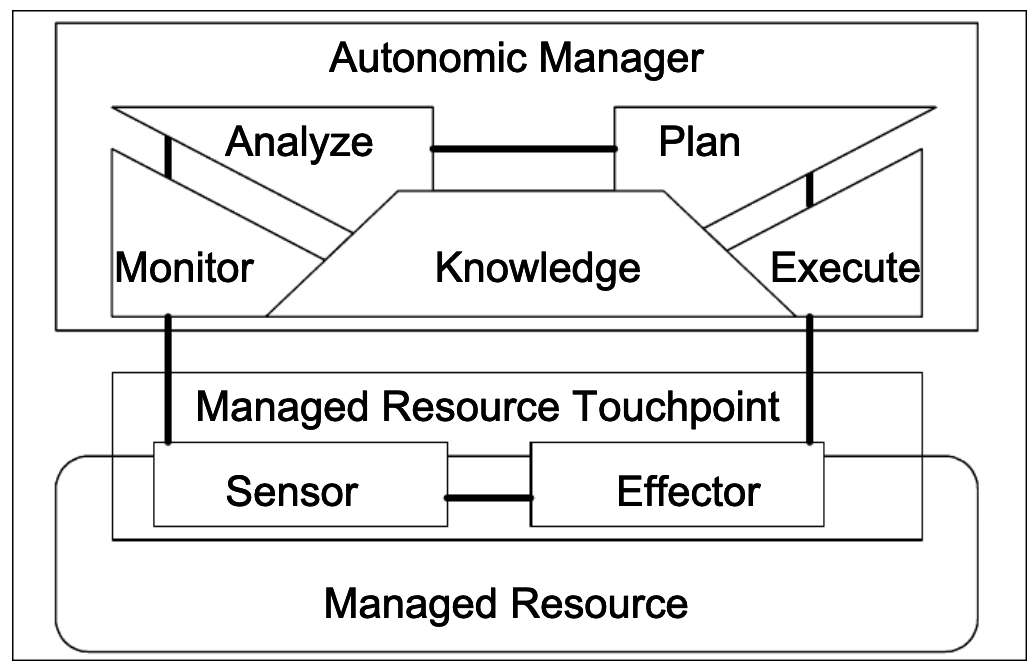
\includegraphics[scale=1]{images/04_technical_background/ac_concept}%
\caption{Autonomic computing concept - Source: Authors own model, based on \cite{Jacob2004AutonomicSolution}.}%
\label{fig:ac_concept}%
\end{figure}

% Figure + short description
\Fig{fig:ac_concept} demonstrates the main concept of an autonomic computing environment. The autonomic computing architecture relies on monitoring sensors and an adoption engine (autonomic manager) to manage resources in the environment \cite{Goscinski2011CloudComputing}.
% About the environment
In an autonomic computing environment, all components have to communicate to each other and can manage themselves. Appropriate decisions will be made by an autonomic manager that knows the given policies \cite{Jacob2004AutonomicSolution}.

% Control loop figure
\begin{figure}[h]%
\centering
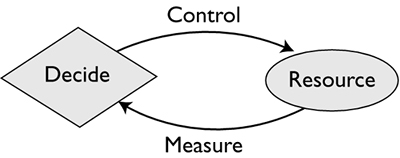
\includegraphics[scale=1]{images/04_technical_background/ac_control_loop}%
\caption{The control-loop concept - Source: Authors own model, based on \cite{Murch2004Autonomic}.}%
\label{fig:ac_control_loop}%
\end{figure}

% Explain control loop
The core element of the autonomic architecture is the control-loop. \Fig{fig:ac_control_loop} illustrates the concept of a control-loop. The control-loop collects details about resources through monitoring and makes decisions based on analysis of the collected details to adjust the system if needed \cite{Murch2004Autonomic}.


\subsection{Managed resources}

% Figure
\begin{figure}[h]%
\centering
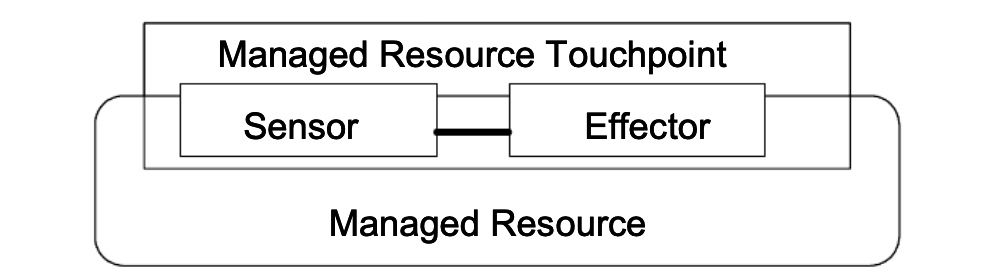
\includegraphics[scale=1]{images/04_technical_background/ac_managed_resource}%
\caption{Managed resource - Source: Authors own model, based on \cite{Jacob2004AutonomicSolution}.}%
\label{fig:ac_managed_resource}%
\end{figure}

% Explanation
A managed resource is a single component or a combination of components in the autonomic computing environment \cite{Murch2004Autonomic, Jacob2004AutonomicSolution}. A component can be a hardware or software component, e.g. a database, a server, an application or a different entity \cite{Sinreich2006AnAB}.
% Sensors and Effectors
They are controlled by their sensors and effectors, as illustrated in \Fig{fig:ac_managed_resource}. Sensors are used to collect information about the state of the resource and effectors can be used to change the state of the resource \cite{Jacob2004AutonomicSolution}. The combination of sensors and effectors is called a touchpoint, which provides an interface for communication with the autonomic manager \cite{Sinreich2006AnAB}.
% Scalability
The ability to manage and control managed resources make them highly scalable \cite{Murch2004Autonomic}.


\subsection{Autonomic manager}
\label{subsec:background-autonomic_computing-autonomic_manager}

% Figure
\begin{figure}[h]%
\centering
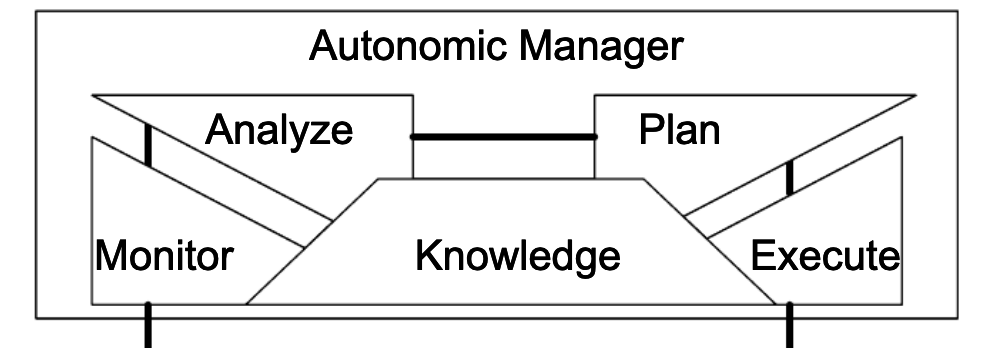
\includegraphics[scale=1]{images/04_technical_background/ac_autonomic_manager}%
\caption{Autonomic manager - Source: Authors own model, based on \cite{Jacob2004AutonomicSolution}.}%
\label{fig:ac_manager}%
\end{figure}

% WHat is the autonomic manager
The autonomic manager implements the control-loop to collect, aggregate, filter and report system metrics from the managed resources. It can only make adjustments within it`s own scope and uses predefined policies to make decisions of what actions have to be executed to accommodate the goals and objectives \cite{Murch2004Autonomic, Sinreich2006AnAB}.
% Knowledge
In addition, the autonomic manager gains knowledge through analyzing the managed resources \cite{Murch2004Autonomic}.
% MAPE-K
The autonomic computing concept digests the MAPE-K model to implement an autonomic manager, as illustrated in \Fig{fig:ac_manager} \cite{Goscinski2011CloudComputing}.

\begin{itemize}
\item \textbf{Monitor:}
The monitor phase is responsible to collect the needed metrics from all managed resources and applies aggregation and filter operations to the collected data \cite{Sinreich2006AnAB}.

\item \textbf{Analyze:}
The autonomic manager has to gain knowledge to determine if changes have to made to the environment \cite{Sinreich2006AnAB}. To predict future situations, the autonomic manager can model complex situation given the collected knowledge \cite{Jacob2004AutonomicSolution}.

\item \textbf{Plan:}
Plans have to be structured to achieve defined goals and objectives. A plan consists of policy-based actions \cite{Jacob2004AutonomicSolution, Sinreich2006AnAB}.

\item \textbf{Execute:}
The execute phase applies all necessary changes to the computing system \cite{Sinreich2006AnAB}.
\end{itemize}

% Multiple manager
Multiple autonomic manager can exist in an autonomic computing environment to perform only certain parts. For example, there can be one autonomic manager which is responsible to monitor and analyse the system and another autonomic manager to plan and execute. To create a complete and closed control-loop, multiple autonomic manager can be composed together \cite{Sinreich2006AnAB}.


% ===========================================
% ===========================================
\section{System Performance}


\subsection{Performance Metrics}
% Short description
Performance metrics are statistics that describe the system performance. These statistics are generated by the system, applications or other tools \cite{Greg2020SysPerf}.
% Common types
The following are examples of common types for performance metrics:
\begin{itemize}
\item \textbf{Throughput:} Volume of data or operations per second \cite{Greg2020SysPerf}.
\item \textbf{Latency:} Time of operation \cite{Greg2020SysPerf}.
\item \textbf{Utilization:} Usage of a component \cite{Greg2020SysPerf}.
\end{itemize}


% Overhead
\paragraph{}Measuring performance metrics can cause an overhead. To gather and store performance metrics, CPU cycles must be spent. This can have a negative affect on the target performance \cite{Greg2020SysPerf}.


\subsection{Time-Based Utilization}
% What is utilization
Utilization is a performance metrics that describes the usage of a device, e.g. CPU device usage.
% What about time-based utilization
A time-based utilization describes the usage of a component during a time period where the component was actively performing work \cite{Greg2020SysPerf}.
% 100% utilization
When a resource approaches 100\% utilization, the performance of that resource can degrade. If a component can process operations in parallel, the performance does not have to degrade much at 100\% utilization and the component can process more work \cite{Greg2020SysPerf}.


% ===========================================
% ===========================================
\section{Monitoring}
% What is monitoring
Monitoring is a process, that aims to detect and take care of system faults. In a dynamic environment, becoming aware of the system is trivial \cite{Ligus2012EffMonitoring}.
% What is a monitoring system
A monitoring system consists of a set of different tools. The tools are responsible to perform measurements on components in the computing environment and collect, store and interpret the monitored data \cite{Ligus2012EffMonitoring}. 


% The monitoring Loop/Process
\begin{figure}[h]
\centering
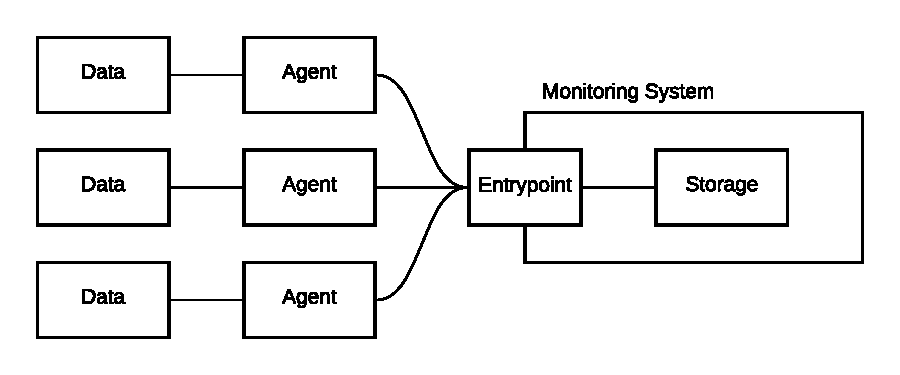
\includegraphics[scale=0.9]{images/02_theoretical_foundation/monitoring/monitoring_system}
\caption{The monitoring process - Source: Authors own model.}
\label{fig:mon_mon-system-process}
\end{figure}
In the monitoring process, illustrated in \Fig{fig:mon_mon-system-process}, data is continuously collected by agents. An agent is a process that continuously gathers metrics. Data can be device statistics, logs or system measurements. Agents will group these data into metrics and submit them to the monitoring system via a protocol. The monitoring system will store the metrics in its database \cite{Ligus2012EffMonitoring}.


% Requirements of a monitoring system
The requirements for a monitoring system, that is able to monitor a dynamic changing environment, are the following:
\begin{itemize}
\item An efficient database to store metrics
\item A decentralized way of generating metrics \cite{Farcic2017Toolkit21} % Neu schreiben
\item Multi-dimensional metrics \cite{Farcic2017Toolkit21}
\item A powerful query language \cite{Farcic2017Toolkit21}
\end{itemize}


\subsection{Database}
% TS are needed
Saving continous data needs to be done efficiently. 
For time-based metrics, a time series database is he most effective way to save the data \cite{Farcic2017Toolkit21}. To store a huge amount of data, data is stored in a very compact format.
A BISL MEHR ÜBER METRICS UND TIMESERIES.


\subsection{Decentralized Way of gathering Metrics}
The approach how the monitoring systems gathers metrics to store in the database plays a significant role.
% There are push and pull based systems
Push and pull based systems are the two primary approaches to gather metrics from services.
% About push
Push based monitoring systems expect services to push metrics to their storage.
% About pull
On the other hand, pull based monitoring systems scrape metrics from all defined targets. Targets do not know about the existence of the monitoring system and only need to collect and expose metrics.


% When to choose what (Discovery)
Service discovery is an important aspect to decide whenever to use a pull or push based monitoring system.

\begin{figure}[h]
\centering
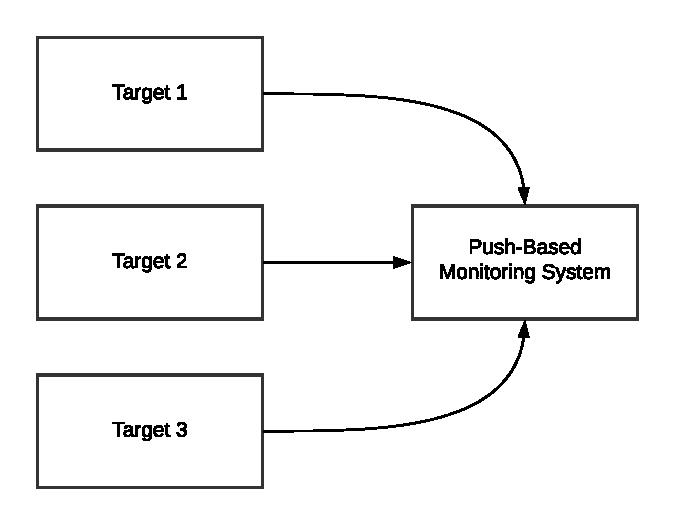
\includegraphics[scale=0.8]{images/02_theoretical_foundation/monitoring/push_based}
\caption{Push-based monitoring approach - Source: Authors own model.}
\label{fig:mon_push-based}
\end{figure}
% Push based discovery
In a push-based environment, services only need to know the address of the monitoring service to push their data to the storage.


\begin{figure}[h]%
\centering
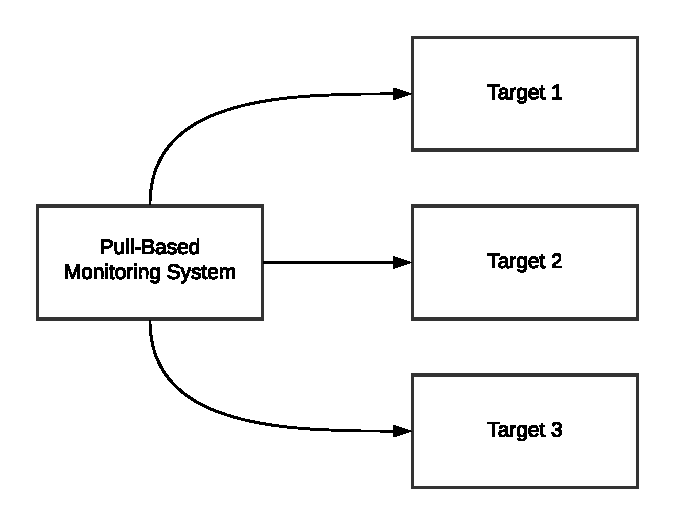
\includegraphics[scale=0.8]{images/02_theoretical_foundation/monitoring/pull_based}%
\caption{Pull-based monitoring approach - Source: Authors own model.}%
\label{fig:mon_pull-based}%
\end{figure}
% Pull based discovery
A pull-based monitoring tool needs to know the address of each target in the environment.
% Why pull based works best with discovery
The advantage of a pull-based systems are, they know what they expect. It is ieasier for pull-based monitoring system to detect whenever a target has failed or is not available.


\subsection{Multi-dimensional Metrics}
% Why do we need dimensions
For query languages to be effective, metrics need to be dimensional. Metric without dimensions, are limited in their capabilities.
% Dynamic environment
In a dynamic environment, services are dynamically added and removed. Therefore, a dynamic environment needs dynamic analytics where metrics represent all dimension in the environment \cite{Farcic2018Toolkit22}.
% Example
\begin{lstlisting}[frame=single, label=lst:mon_metr_dimless, caption=Example of a dimensionless-metric, captionpos=b]
container_memory_usage
\end{lstlisting}
\begin{lstlisting}[frame=single, label=lst:mon_metr_withdim, caption=Example of a metric with dimensions, captionpos=b]
container_memory_usage{service="my_service"}
\end{lstlisting}
% Explain
As the exasmple \Lst{lst:mon_metr_dimless} and \Lst{lst:mon_metr_withdim} show, the metric with dimension provide more efficient querieing to gather informations about the environment.


\subsection{Query Language}



\subsection{Choosing a Monitoring Tool}
Graphite or Prometheus, Prometheus it its! <- Eher in Design

\chapter{Related Work}
\label{chap:03_related-work}


This chapter provides an overview of related literature for this thesis. Furthermore, the surveyed literature is built on the theoretical foundation introduced in \Chap{chap:02_foundation}. This chapter introduces work about auto-scaling computing environments, GPU accelerated Apache Spark cluster, and the implementation of an automated deployment pipeline. These topics are related to the choice of technologies (\Chap{chap:04_background}), the proposed conceptual design of this thesis (\Chap{chap:05_design}), and the resulting implementation (\Chap{chap:06_implementation}).


% ===========================================
% ===========================================
\section{Auto-Scaling Computing Environments}
% State of the art monitoring
In recent years, container technologies have been used efficiently in complex computing environments. Dynamic scaling of containerized applications is an active area of research.
% WHich is important for this thesis
To accommodate this thesis research objective, the literature research according to auto-scaling environments was focused on two topics: Concepts of \textit{Auto-Scalers}  and auto-scaling algorithms.


\subsection{Auto-Scaler Concepts}
% A review of auto-scaling techniques for elastic application in cloud environments
\paragraph{}
Lorido-Botrán et al. \cite{Lorido2014Review} reviewed state-of-the-art literature about auto-scaling and explain auto-scaling process proposals in a cloud environment.
% SLA and costs
It is mentioned that an \textit{Auto-Scaler} is responsible to find a trade-off between meeting the Service Level Agreement (\hyperlink{abbr:sla}{SLA}) and keeping the cost of renting resources low.
% SLA
Two types of \hyperlink{abbr:sla}{SLA} exists while maintaining an acceptable trade-off: The application \hyperlink{abbr:sla}{SLA} and the resource \hyperlink{abbr:sla}{SLA}. The former is a contract between the application owner and the end-users (e.g., a certain response time). The resource \hyperlink{abbr:sla}{SLA} is agreed upon by the infrastructure provider and the application owner (e.g., 99.9\% availability).
% Auto-scaling problems
They introduced three problems \textit{Auto-Scaler} faces while scaling an environment and meeting the \hyperlink{abbr:sla}{SLA}:
% The problems
\begin{enumerate}
%1
\item Under-provisioning:
An application is under-provisioned if it needs more resources to process the incoming workload.
To make resources available and return the application to its normal state may take some time, which causes \hyperlink{abbr:sla}{SLA} violations.
% 2
\item Over-provisioning:
Applications with more resources available than needed will lead to unnecessary costs for the client.
% 3
\item Oscillation:
If scaling-actions are executed too quickly before the impact is available, a combination of over-provisioned and under-provisioned applications can occur.
A cooldown period after a scaling-action allows preventing oscillation.
\end{enumerate}
% MAPE
To prevent the mentioned problems from occurring, the authors introduced and explained the \hyperlink{abbr:mape}{MAPE} architecture (cf. \Sec{sec:02_ac}).
% MAPE phases
\hyperlink{abbr:mape}{MAPE} consists of four different phases: Monitor, Analyse, Plan, and Execute.
% Only AP
There exist \textit{Auto-Scaler} proposals which only focus on the Analyse, and Planning phase architecture of the \hyperlink{abbr:mape}{MAPE} architecture.
% Analysing and planning techniques
Several techniques for the Analyse phase are being introduced: Queuing theory and time-series analysis.
As well as for the planning phase: Threshold-based rules, reinforcement learning, and control theory.
% Active proactive grouping
There exist \textit{Auto-Scaler} which uses techniques to predict the future state of the environment (e.g., reinforcement learning). These are called proactive \textit{Auto-Scalers}.
Reactive \textit{Auto-Scalers} use techniques to respond to the environment's current status (e.g., threshold-based rules).


% Application deployment using containers with auto-scaling for microservices in cloud environment
\paragraph{}
Srirama et al. \cite{Srirama2020AppDeplyCont} designed a heuristic-based auto-scaling strategy for container-based microservices in a cloud environment. The purpose of the auto-scaling strategy is to balance the overall resource utilization across microservices in the environment.
% Results
The proposed auto-scaling strategy performed better than state-of-the-art algorithms in processing time, processing cost, and resource utilization. The processing cost of microservices was reduced by 12-20\%. The \hyperlink{abbr:cpu}{CPU} and memory utilization of cloud-servers were maximized by 9-15\% and 10-18\%, respectively.


% Comparison of auto-scaling techniques for cloud environments
\paragraph{}
Lorido-Botrán et al.  \cite{Botran2013AutoScalingComp} compared different representative auto-scaling techniques in a simulation in terms of cost and \hyperlink{abbr:sla}{SLA} violations. They compared load balancing with static threshold-based rules, reactive and proactive techniques based on \hyperlink{abbr:cpu}{CPU} load.
Load balancing is based on static rules defining the upper and lower thresholds of a specific load (e.g., \textit{if CPU > 80\% then scale-out; if CPU < 20\% then scale-in}). The difficulty of this technique is to set the ideal rules. False rules can lead to bad performance. Proactive techniques try to predict the future values of performance metrics based on historical data. Reactive techniques are based on control theory to automate the system management. To overcome the difficulties of static thresholds, the authors proposed a new auto-scaling technique using rules with dynamic thresholds. The results showed that for auto-scaling techniques to scale well, it highly depends on parameter tuning. The best result was achieved with proactive results with a minimum threshold of 20\% and a maximum of 60\%.


\subsection{Auto-Scaling Algorithms}
% Delivering elastic ...
\paragraph{}Barna et al. \cite{Barna2017ElasticContainerApps} proposed an autonomic scaling architecture approach for containerized microservices. Their approach focused on creating an autonomic management system, following the autonomic computing concept \cite{Kephart2003VisionComputing}, using a self-tuning performance model. The demonstrated architecture frequently monitors the environment and gathers performance metrics from components. It can analyze the data and dynamically scale components. In addition, to determine if a scaling action is needed, they proposed the \textit{Scaling Heat Algorithm}. The Scaling Heat algorithm is used to prevent unnecessary scaling actions, which can throw the environment temporarily off.
% Is ised in this thesis
The Scaling Heat algorithm will be used for decision making in this thesis and is explained in detail in \Sec{sec:04_background_scaling-heat}.


% Auto-scaling of Containers: the Impact of Relative and Absolute Metrics
\paragraph{}Casalicchio et al. \cite{Casalicchio2017AutoScaleCont} focused on the difference of absolute and relative metrics for container-based auto-scaling algorithms. They analysed the mechanism of the \textit{Kubernetes Horizontal Pod Auto-Scaling} (\hyperlink{abbr:khpa}{KHPA}) algorithm and proposed a new auto-scaling algorithm based on \hyperlink{abbr:khpa}{KHPA} using absolute metrics called \textit{KHPA-A}. The results showed that KHPA-A could reduce response time between 0.5x and 0.66x compared to \hyperlink{abbr:khpa}{KHPA}. In addition, their work proposed an architecture using cAdvisor for collecting container performance metrics, Prometheus for monitoring, alerting, storing time-series data, and Grafana for visualizing metrics. 
% KHPA
Absolute metrics are more appropriate when it comes to efficient resource allocation. Therefore, the KHPA-A algorithm is more efficient in vertical scaling of resources.
% This thesis
In this thesis, the focus for scaling strategies is based on the horizontal scaling approach. Therefore, the \hyperlink{abbr:khpa}{KHPA} algorithm will be used throughout this thesis and is explained in detail in \Sec{sec:04_background_khpa}.


% ===========================================
% ===========================================
\section{GPU accelerated Apache Spark Cluster}
% Short intro
This thesis aims to enable \hyperlink{abbr:gpu}{GPU} acceleration for Apache Spark.
% Research
In research, many solutions have been proposed which try to solve the problem in similar ways.
% Following
In the following, three different approaches are introduced.


% HeteroSpark
\paragraph{}
Li et al. \cite{Li2015HeteroSpark} developed a middleware framework called \textit{HeteroSpark} to enable \hyperlink{abbr:gpu}{GPU} acceleration on Apache Spark worker nodes. HeteroSpark listens for function calls in Apache Spark applications and invokes the \hyperlink{abbr:gpu}{GPU} kernel for acceleration. For communication between \hyperlink{abbr:cpu}{CPU} and \hyperlink{abbr:gpu}{GPU}, HeteroSpark implements a \hyperlink{abbr:cpu}{CPU}-\hyperlink{abbr:gpu}{GPU} communication layer for each worker node using the Java Remote Method Invocation (\hyperlink{abbr:rmi}{RMI}) \hyperlink{abbr:api}{API}. To execute operations on the \hyperlink{abbr:gpu}{GPU}, the \hyperlink{abbr:cpu}{CPU} Java Virtual Machine (\hyperlink{abbr:jvm}{JVM}) will send serialized data to the \hyperlink{abbr:gpu}{GPU} JVM using the \hyperlink{abbr:rmi}{RMI} communication interface. The \hyperlink{abbr:gpu}{GPU} \hyperlink{abbr:jvm}{JVM} will deserialize the received data for execution.
% Design
The design provides a plug-n-play approach and an \hyperlink{abbr:api}{API} for the user to call functions with \hyperlink{abbr:gpu}{GPU} support.
% Results
Overall, HeteroSpark is able to achieve an 18x speed-up for various Machine Learning applications running on Apache Spark.


% HetSpark
\paragraph{}
Klodjan et al. \cite{Klodjan2018HetSpark} introduced \textit{HetSpark}, a modification of Apache Spark.
% The goal
HetSpark extends Apache Spark with two executors, a \hyperlink{abbr:gpu}{GPU} accelerated executor and a commodity class. 
% accelerated
The accelerated executor uses VineTalk\cite{Mavridis2017VineTalk} for \hyperlink{abbr:gpu}{GPU} acceleration.
% VineTalk
VineTalk contributes as a transport layer between the application and accelerator devices (\hyperlink{abbr:cpu}{CPU} or \hyperlink{abbr:gpu}{GPU}).
% Byte code analysis
To detect suitable tasks for \hyperlink{abbr:gpu}{GPU} acceleration, HetSpark uses the ASM\footnote{ASM - \url{https://asm.ow2.io/} (Accessed: 2021-01-11)} framework to analyse the byte code of Java binaries.
% Results
The authors observed that for compute-intensive tasks, \hyperlink{abbr:gpu}{GPU} accelerated executers are preferable, while for linear tasks, \hyperlink{abbr:cpu}{CPU}-only accelerators should be used.


% Spark-GPU
\paragraph{}
% SHort intro
Yuan et al. \cite{Yuan2016SparkGPU} proposed \textit{SparkGPU} a \hyperlink{abbr:cpu}{CPU}-\hyperlink{abbr:gpu}{GPU} hybrid system built on top of Apache Spark.
% The goal
The goal of SparkGPU is to utilize \hyperlink{abbr:gpu}{GPUs} to achieve high performance and throughput.
% Problems trying to solve
SparkGPU tries to solve the following problems statements:
% The problems
\begin{enumerate}
% Iterator
\item The iterator model of Apache Spark executes one element at a time.
This approach does not match the \hyperlink{abbr:gpu}{GPU} architecture and underutilizes \hyperlink{abbr:gpu}{GPU} resources.

% JVM
\item Apache Spark runs on the \hyperlink{abbr:jvm}{JVM} and therefore stores its data on the heap memory.
\hyperlink{abbr:gpu}{GPU} programs are usually implemented with \hyperlink{abbr:gpu}{GPU} programming models like Compute Unified Device Architecture (\hyperlink{abbr:cuda}{CUDA}), which cannot access data on the heap.
Therefore, data must be copied between the heap and native memory frequently. These copy operations are expensive.

% Cluster manager
\item Existing cluster manager of Apache Spark manage \hyperlink{abbr:gpu}{GPUs} in a coarse-grained fashion.
This can lead to crashes because of insufficient memory when multiple programs run on the \hyperlink{abbr:gpu}{GPU} concurrently.
\end{enumerate}
% Extension
To solve the mentioned problem statements, SparkGPU extends Apache Spark in the following ways:
\begin{itemize}
\item Enable block processing on \hyperlink{abbr:gpu}{GPUs} by extending the Apache Sparks iterator model. Therefore Apache Spark can better utilize \hyperlink{abbr:gpu}{GPUs} to accelerate application performance.

\item To offload queries to the \hyperlink{abbr:gpu}{GPU}, SparkGPU extends the query optimizer. The query optimizer will create query plans with both \hyperlink{abbr:cpu}{CPU} and \hyperlink{abbr:gpu}{GPU} operators.

\item To manage \hyperlink{abbr:gpu}{GPUs} efficiently, SparkGPU extends the cluster manager and the task scheduler.
\end{itemize}
% Intro GPU-RDD
To extend the programming \hyperlink{abbr:api}{API}, SparkGPU provides a new Resilient Distributed Dataset (\hyperlink{abbr:rdd}{RDD}) type called GPU-RDD.
% OPtimized for GPU
A GPU-RDD is optimized to utilize the \hyperlink{abbr:gpu}{GPU}.
SparkGPU utilizes native memory on the \hyperlink{abbr:gpu}{GPU} instead of the Java heap to buffer data in GPU-RDDs.
% Operations
Operations performed on a GPU-RDD can be performed on the \hyperlink{abbr:gpu}{GPU}. Several built-in operators on the GPU-RDD are provided, which support data-parallelism.


% The query optimizer
SparkGPU can execute Structured Query Language (\hyperlink{abbr:sql}{SQL}) queries on both \hyperlink{abbr:cpu}{CPU} and \hyperlink{abbr:gpu}{GPU}.
By adding a set of \hyperlink{abbr:gpu}{GPU} rules and strategies, SparkGPU extends the query optimizer to find the best execution plan for \hyperlink{abbr:gpu}{GPU} scheduling.

% Cluster manager
To manage \hyperlink{abbr:gpu}{GPU} memory on shared \hyperlink{abbr:gpu}{GPUs}, SparkGPU provides a user-level \hyperlink{abbr:gpu}{GPU}-management library.
% Mem contention
When memory contention happens, the library will ensure that SparkGPU will stop scheduling new tasks to the Apache Spark cluster.

% End
SparkGPU accomplished to improve the performance of machine learning algorithms up to 16.13x and \hyperlink{abbr:sql}{SQL} query execution performance up to 4.83x.


% ===========================================
% ===========================================
\section{Implementation of an Automated Deployment Pipeline}
Implementing an automated deployment pipeline is a more applied topic and well described in many literatures. In this sections the primary literature used throughout the implementation of this thesis work is being introduced.


% continuous delivery
\paragraph{}The conceptual design and implementation of an automated deployment pipeline in this thesis were mostly inspired by the proposed solution of the book \textit{Continuous Delivery: Reliable Software Releases through Build, Test, and Deployment Automation} by Humble et al. \cite{Farley2010CI}.
% Short intro about the content of this book
The authors explain the theoretical idea behind an automated deployment pipeline and explaining an example implementation.
% Implementation
The proposed implementation covers the software lifecycle from compiling source code to delivering the software to a production environment.
The commit stage, which covers the build and test part of the software, can be applied in parts for this thesis work.

\chapter{Technical Background}
\label{chap:04_background}

This chapter provides information about the technologies and algorithms used for the conceptual design (\Chap{chap:05_design}) and implementation (\Chap{chap:06_implementation}) of this thesis. It explains the fundamental concepts of Docker, Apache Spark, RAPIDS accelerator plugin, Prometheus, cAdvisor, DCGM-Exporter, and GitLab CI/CD. Additionally, the Scaling Heat and Kubernetes Horizontal Pod Autoscaler algorithms are introduced.

% ===========================================
% ===========================================
% Docker
% ===========================================
% ===========================================
\section{Docker}
\label{sec:04_docker}
% Short docker intro
Docker is an open-source platform that enables the containerization of applications. Containerization is a technology to package, ship, and run applications and their environment in individual containers.
% Make clear
Docker is not a container technology itself. It hides the complexity of working with container technologies directly and instead provides an abstraction and the tools to work with containers \cite{Nickoloff2019Docker, Bullington2020Docker, Potdar2020Docker}.


\subsection{Docker Architecture}
\label{subsec:04_docker_architecture}
% Architecture figure
\begin{figure}[h]
\centering
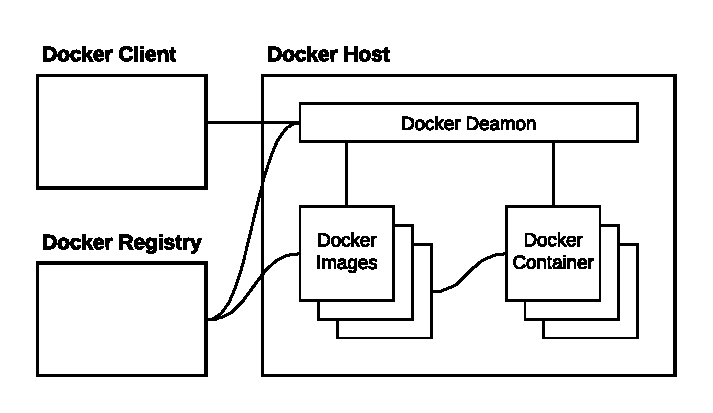
\includegraphics[scale=1]{images/04_technical_background/docker/docker_architecture}
\caption{Docker architecture - Source: Authors own model, based on \cite{Docker2020Docs}.}
\label{fig:04_docker_architecture_architecture}
\end{figure}

% Explain figure
\Fig{fig:04_docker_architecture_architecture} illustrates the client-server architecture of Docker. It consists of a Docker Client, the Docker Deamon, and a Docker Registry.

\begin{itemize}
% Docker client
\item Docker Client: The Docker client is an interface for the user to send commands to the Docker daemon \cite{Docker2020Docs}.

% Docker deamon
\item Docker Deamon: The Docker daemon manages all containers running on the host system and handles container resources, networks and, volumes \cite{Bullington2020Docker}.

% Docker registry
\item Docker Registry: A Docker registry stores images. Images can be pushed to or pulled from public or private registries to build a container \cite{Docker2020Docs}.
\end{itemize}


\subsection{Docker Image}
\label{subsec:04_docker_image}
\paragraph{}
% What is an image
An Image is a snapshot of the environment to run an application in a Docker container. The environment consists of all files, libraries, and configurations that are needed for the application to run correctly \cite{Docker2020Docs, Nickoloff2019Docker}.
% How to create an image
Images can be created from existing containers or from executing a build script called \textit{Dockerfile} \cite{Nickoloff2019Docker}.


\paragraph{}
Images can be built automatically by executing a build script called Dockerfile, a text document that contains specific build instructions. Instructions are commands which are executed in order to assemble an image.
% Parent
A Dockerfile must begin with a \texttt{FROM} instruction which defines the parent image from which the image is built \cite{Docker2020Docs}.


% Example
\Lst{lst:04_docker_image_dockerfile} provides a basic example of a Dockerfile.
% Parent
In the example, \textit{ubuntu} is defined as the parent image at line 1.
% apt
Next, from 3 to 4, the Ubuntu package list is updated, and the \textit{nginx} package is installed using the \texttt{apt-get} command.
% Expose
Finally, at line 6, the Docker image is instructed to listen to port 80 at runtime with the \texttt{EXPOSE} instruction.

% Dockerfile example
\begin{lstlisting}[label=lst:04_docker_image_dockerfile, caption=Basic example of a Dockerfile]
FROM ubuntu

RUN apt-get update -qy && \
    apt-get install -y nginx

EXPOSE 80
\end{lstlisting}


\subsection{Docker Container}
% What are containers
A container is an execution environment running on the host-system kernel.

% Container image
\begin{figure}[h]
\centering
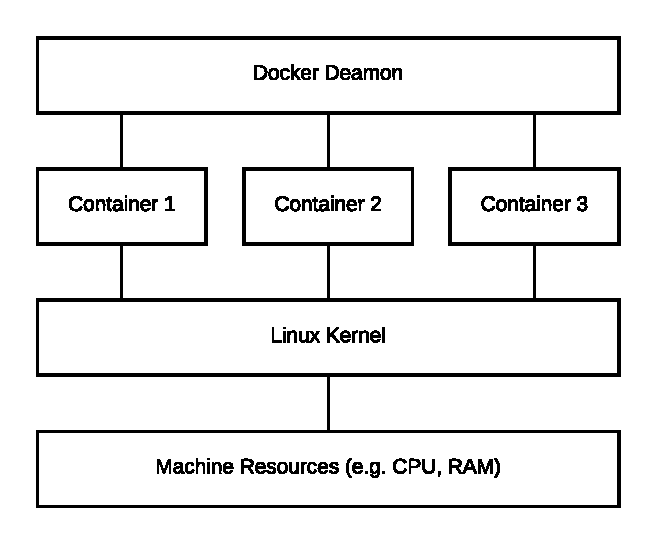
\includegraphics[scale=1]{images/04_technical_background/docker/container_structure}
\caption{Docker basic container structure - Source: Authors own model, based on \cite{Bullington2020Docker}.}
\label{fig:04_docker_container_container-structure}
\end{figure}

% Container advantages
The advantage of a container is its lightweight nature. As illustrated in \Fig{fig:04_docker_container_container-structure}, containers take advantage of \hyperlink{abbr:os}{OS}-level virtualization instead of hardware-virtualization without the need for a hypervisor \cite{Docker2020Docs, Nickoloff2019Docker}. Containers share the resources of the host system instead of using reserved resources \cite{Bullington2020Docker}. Multiple containers can run on the host-system kernel and are by default isolated from each other \cite{Docker2020Docs}.
% Docker container
In Docker, a container is a runnable unit of an image used to distribute and test applications. A container can be configured to expose specific resources to the host system, e.g., network ports \cite{Bullington2020Docker}.


\subsection{Docker Swarm Mode}
\label{subsec:04_docker_swarm}
% What is Docker swarm
Docker Swarm mode is the native cluster orchestration and management tool embedded in the Docker Engine.
% What is a swarm
In Docker Swarm mode, a cluster of multiple nodes is called a swarm. All nodes run in Swarm mode and act as managers or workers.
% Whats the purpose
In a swarm, multiple services can be deployed. The manager node is responsible for maintaining the desired state of a service \cite{Docker2020Docs}.


% 
Many properties of Docker Swarm mode contribute the fact that it is an ideal tool to create a self-healing and self-adapting environment:
\begin{itemize}
\item Desired state: The manager node monitors each service's state in the swarm and adapts the environment to maintain the desired state\cite{Docker2020Docs}.

\item Cluster management and orchestration: Docker Swarm mode is integrated within the Docker Engine. A swarm can be created and managed using the Docker command-line interface (\hyperlink{abbr:cli}{CLI}) \cite{Docker2020Docs}.

\item Service model: The Docker Engine allows to define the desired state of a service. The manager node maintains the desired state of all services in the swarm \cite{Docker2020Docs}.

\item Scaling: The number of replicas is defined for each service. The manager node automatically adapts the number of replicas for a service to keep the desired state \cite{Docker2020Docs}.

\item Multi-host networking: A swarm runs all services in an overlay network, and new services will automatically be added to it \cite{Docker2020Docs}.
\end{itemize}


\subsubsection{Services and Tasks}
% What is a service
A service defines the desired state of a task. The state is defined by the number of replicas of a service and the configuration for the Docker container, e.g., Docker image, resources, network, and more \cite{Docker2020Docs}.


%What is a node
A task is a running Docker container. The task is defined by the corresponding service and is managed by the manager node. A task can be executed on worker and manager nodes \cite{Docker2020Docs}.


\subsubsection{Nodes}
% What is a node
A Docker engine participating in the swarm is called a node.
% What about the node role
Nodes can act as manager nodes, worker nodes, or both \cite{Docker2020Docs}.


% What about the manager
The manager node is responsible for cluster orchestration and management. It maintains the desired state of all services and tasks in the swarm. In addition, the manager node dispatches tasks to worker nodes when service definitions are submitted to the manager node \cite{Docker2020Docs}.


% What about worker
Worker nodes are responsible for executing the tasks received by the manager node. While performing tasks, the worker node notifies the manager node about each task state \cite{Docker2020Docs}.


\subsubsection{Stack}
%
A stack is a named collection of first-class Docker resources (e.g., services, volumes, networks) that can be deployed to a swarm.
%
The docker-compose file format allows describing a stack in a single \hyperlink{abbr:yaml}{YAML}\footnote{YAML Ain't Markup Language - \url{https://yaml.org/} (Accessed: 2021-02-18)} file. With the \texttt{docker stack} command, a docker-compose file can be used to create a stack and deploy it to a swarm.
% Example
\Lst{lst:04_docker_swarm_stack_compose} provides an example of a stack described in the docker-compose file format.
% Explain
It defines two services called \textit{prometheus} and \textit{cadvisor}. Both services are attached to the \textit{computing-net} network.
\begin{lstlisting}[label=lst:04_docker_swarm_stack_compose, caption=Basic example of stack describes in the docker-compose file format]
version: "3.7"

networks:
    computing-net:
        name: computing_net

services:
    prometheus:
        image: prom/prometheus:latest
        networks:
            - computing-net
            
    cadvisor:
        image: google/cadvisor:latest
        networks:
            - computing-net        
\end{lstlisting}
% Deploy
\Lst{lst:04_docker_swarm_stack_deploy} shows the usage of the \texttt{docker stack} command. It deploys a stack with the name \textit{computing-stack} using a docker-compose file.
\begin{lstlisting}[label=lst:04_docker_swarm_stack_deploy, caption=Usage of the docker stack command to deploy a stack, language=bash, numbers=none]
$ docker stack deploy -c computing-stack.yml computing-stack     
\end{lstlisting}


% ===========================================
% ===========================================
% Apache Spark
% ===========================================
% ===========================================
\section{Apache Spark}
\label{sec:04_spark}
Apache Spark is an open-source computing framework for parallel data processing on a large computer cluster. Apache Spark manages the available resources and distributes computation tasks across a cluster to perform big-data processing operations at a large scale \cite{Chambers2018Spark}. Before Apache Spark was developed, Hadoop MapReduce \cite{Dean2010MapReduce} was the framework of choice for parallel operations on a computer cluster \cite{Zaharia2010Spark}. However, Spark accomplished to outperform Hadoop by 10x for iterative Machine Learning \cite{Zaharia2010Spark} and is now one of the most popular frameworks for distributed computing. It is implemented in Scala\footnote{The Scala programming language - \url{https://www.scala-lang.org/} (Accessed: 2020-12-18)}, a \hyperlink{abbr:jvm}{JVM}-based programming language. It provides a programming interface for Scala, Java\footnote{Java Software - \url{https://www.oracle.com/java/} (Accessed: 2020-12-18)}, Python\footnote{Python programming language - \url{https://www.python.org/} (Accessed: 2020-12-18)}, and R\footnote{The R Project for Statistical Computing - \url{https://www.r-project.org/} (Accessed: 2020-12-18)}. Additionally, Apache Spark includes an interactive \hyperlink{abbr:sql}{SQL} shell and libraries to implement \hyperlink{abbr:ml}{ML} and streaming applications \cite{Chambers2018Spark}.


\subsection{Spark Programming Model}
\label{subsec:04_spark_pr-model}
% Explain RDDs
Apache Spark provides Resilient Distributed Datasets (\hyperlink{abbr:rdd}{RDDs}) as the main abstraction for parallel operations \cite{Zaharia2010Spark}. Core types of the higher-level structured \hyperlink{abbr:api}{API} are built on top of \hyperlink{abbr:rdd}{RDDs}) and are automatically optimized by the Catalyst optimizer to run operations quickly and efficient \cite{Chambers2018Spark, Hien2018Spark}.


\subsubsection{Apache Spark Structured API}
% What is the structured API
Apache Spark provides high level structured \hyperlink{abbr:api}{APIs} for manipulating all kinds of data. The three distributed core types are Datasets, DataFrames, and \hyperlink{abbr:sql}{SQL}) Tables and Views \cite{Chambers2018Spark}.
% About DataFrames, Datasets and SQL
Datasets and DataFrames are immutable, lazy evaluated collections that provide execution plans for operations \cite{Chambers2018Spark}. \hyperlink{abbr:sql}{SQL} Tables and Views work the same way as DataFrames, except that \hyperlink{abbr:sql}{SQL} is used as the interface instead of using the DataFrame programming interface \cite{Chambers2018Spark}.
% Differences between Datasets ad Dataframes
Datasets use \hyperlink{abbr:jvm}{JVM} types and are therefore only available for \hyperlink{abbr:jvm}{JVM} based languages. DataFrames are Datasets of type \texttt{Row}, which is the optimized format for computations \cite{Chambers2018Spark}.


\subsubsection{Resilient Distributed Datasets}
% What are RDDs
Resilient Distributed Datasets are fault-tolerant, parallel data structures to enable data sharing across cluster applications \cite{Zaharia2012RDDs}. They express different cluster programming models like MapReduce, \hyperlink{abbr:sql}{SQL}, and batched stream processing \cite{Zaharia2012RDDs}. \hyperlink{abbr:rdd}{RDDs} have been implemented in Apache Spark and serve as the Spark structured \hyperlink{abbr:api}{API's} underlying data structure \cite{Zaharia2012RDDs}.
% How can RDDs be used in applications
\hyperlink{abbr:rdd}{RDDs} are an immutable, partitioned collection of records. They can only be initiated through transformations (e.g., map, filter) on data or other \hyperlink{abbr:rdd}{RDDs}.
% What are the advantages of RDDs
An advantage of \hyperlink{abbr:rdd}{RDDs} is that they can be recovered through lineage. Lost partitions of an \hyperlink{abbr:rdd}{RDD} can be recomputed from other \hyperlink{abbr:rdd}{RDDs} in parallel on different nodes \cite{Zaharia2012RDDs}. 
% Better use structured API
\hyperlink{abbr:rdd}{RDDs} are lower-level \hyperlink{abbr:api}{APIs} and should only be used in applications if custom data partitioning is needed \cite{Chambers2018Spark}. It is recommended to use Sparks structured \hyperlink{abbr:api}{API} objects instead. Optimizations for \hyperlink{abbr:rdd}{RDDs} have to be implemented manually, while Apache Spark automatically optimizes the execution for structured \hyperlink{abbr:api}{API} operations \cite{Chambers2018Spark}.


\subsubsection{Apache Spark Catalyst}
\label{subsubsec:04_spark_pr-model_catalyst}
% What is the Catalyst optimizer
Apache Spark also provides a query optimizer engine called Apache Spark Catalyst. \Fig{fig:04_spark_pr-model_catalyst_process} illustrates how Spark Catalyst automatically optimizes Apache Spark applications to run quickly and efficient.
% Short How
Before executing the user code, the Catalyst optimizer translates the data-processing logic into a logical plan and optimizes it using heuristics such as rules \cite{Hien2018Spark}. After that, the Catalyst optimizer converts the logical plan into a physical plan to create executable code \cite{Hien2018Spark}.


% What are logical plans
Logical plans are created from a DataFrame or a \hyperlink{abbr:sql}{SQL} query and represent the data-processing logic as a tree of operators and expressions where the Catalyst optimizer can apply sets of rule-based and cost-based optimizations \cite{Hien2018Spark}.

% What are physical plans
From the logical plan, the Catalyst optimizer creates more physical plans consisting of \hyperlink{abbr:rdd}{RDD} operations \cite{Chambers2018Spark}. The cheapest physical plan will be generated into Java bytecode for execution across the cluster \cite{Hien2018Spark}.

% Spark Catalyst figure
\begin{figure}[h]
\centering
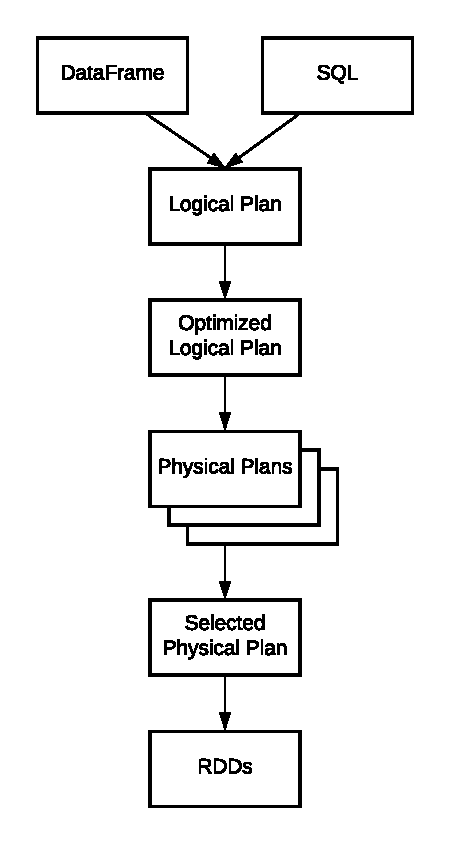
\includegraphics[scale=1]{images/04_technical_background/spark/catalyst_optimization_process}
\caption{Optimization process of the Spark Catalyst - Source: Authors own model, based on \cite{Hien2018Spark}.}
\label{fig:04_spark_pr-model_catalyst_process}
\end{figure}


\subsection{Application Architecture}
\label{subsec:04_spark_architecture}

\begin{figure}[h]
\centering
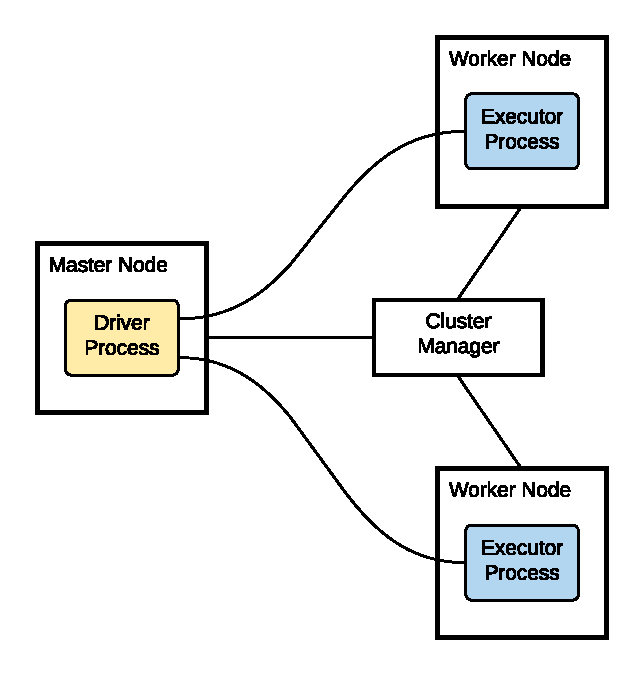
\includegraphics[scale=1]{images/04_technical_background/spark/spark_cluster_architecture}
\caption{Overview of a Spark cluster architecture - Source: Authors own model, based on \cite{Apache2020Spark}.}
\label{fig:spark_cluster_overview}
\end{figure}

% Explain image
\Fig{fig:spark_cluster_overview} illustrates the main architecture of an Apache Spark cluster running an application.
% Master-Worker
The architecture follows the master-worker model.
% The processes
Each running application has one driver process (master) and multiple executor processes (worker) exclusively assigned by the cluster manager.
% Cluster manager
Furthermore, the cluster manager decides on which nodes the processes will be executed \cite{Hien2018Spark}.


\subsubsection{Driver Process}
\label{subsubsec:04_spark_architecture_driver}
The driver process is a \hyperlink{abbr:jvm}{JVM} process running on a physical machine and is responsible for maintaining the execution of an Apache Spark application \cite{Chambers2018Spark}. It coordinates the application tasks and schedules them on available executors \cite{Hien2018Spark}. 
The driver interacts with the cluster manager to launch executors and allocate hardware resources \cite{Chambers2018Spark, Hien2018Spark}.


\subsubsection{Executor Process}
% JVM
The executor process is a \hyperlink{abbr:jvm}{JVM} process that runs through the whole duration of an application \cite{Hien2018Spark, Apache2020Spark}.
% Tasks
It is responsible for performing all tasks (units of work) assigned by the driver process \cite{Chambers2018Spark}.
% Report
After the executor process finishes, it reports back to the driver process \cite{Chambers2018Spark}.
% CPU
Each task is performed on a separate \hyperlink{abbr:cpu}{CPU} core to enable parallel processing \cite{Hien2018Spark}.


\subsubsection{Cluster Manager}
\label{subsubsec:04_spark_architecture_manager}
The cluster manager is an external service that orchestrates the work between available machines in the cluster \cite{Hien2018Spark, Apache2020Spark}.
% Worker and master nodes
It decides on which nodes the driver- and executor processes are launched in the cluster.
% Resources
Additionally, the cluster manager maintains each node's resources in the cluster \cite{Hien2018Spark, Chambers2018Spark}.
% Different cluster types
Apache Spark supports different services that can run as cluster manager, such as Standalone mode (introduced in \Sec{subsec:04_spark_standalone}), Apache Mesos\footnote{Apache Mesos - \url{https://mesos.apache.org/} (Accessed: 2021-01-02)}, Hadoop YARN\cite{Murthy2013Yarn}, and Kubernetes\footnote{Kubernetes - \url{https://kubernetes.io/} (Accessed: 2021-01-02)} \cite{Apache2020Spark}.
% Explain different cluster deploy modes
The cluster manager provides three different deploy modes for acquiring resources in the cluster.
\begin{itemize}
% Cluster mode
\item Cluster mode:
To run an application in cluster mode, the user must submit a precompiled Java ARchive (\hyperlink{abbr:jar}{JAR}), python script, or R script to the cluster manager \cite{Chambers2018Spark}. After that, the cluster manager starts the driver process and executor processes exclusively for the Apache Spark application on machines inside the cluster \cite{Chambers2018Spark, Hien2018Spark}.

% Client mode
\item Client mode:
The difference between the client mode and the cluster mode is that, the driver process runs on the client machine outside of the Spark cluster \cite{Chambers2018Spark}.

% Local mode
\item Local mode:
The local mode starts an Apache Spark application on a single computer \cite{Chambers2018Spark}. It is important to mention that the local mode is not recommended to use in production. Instead, it should be used for testing Apache Spark applications \cite{Chambers2018Spark}.
\end{itemize}


\subsection{Standalone Cluster Deployment}
\label{subsec:04_spark_standalone}
% What is a standalone cluster
The standalone mode is a basic cluster-manager build specifically for Apache Spark. It is developed only to run Apache Spark but supports workloads at a large scale \cite{Chambers2018Spark}.
% Why standalone cluster mode, advantages


\subsubsection{Starting Master and Worker Nodes}
\paragraph{}
Apache Spark provides executable launch scripts to start master and worker nodes in standalone mode.
% Where to find them
Inside the Apache Spark installation directory, the executables can be found at \texttt{sbin/start-master.sh} to start a master node and at \texttt{/start-slave.sh} to start a worker node.
% parameter for worker script
The worker launch executable requires the master node Uniform Resource Identifier (\hyperlink{abbr:uri}{URI}) as a parameter \cite{Apache2020Spark}. 


% Example master
\begin{lstlisting}[label=lst:04_spark_standalone_launch-master, caption=Usage of master launch script, language=bash, numbers=none]
$ ./sbin/start-master.sh
\end{lstlisting}


% Example worker
\begin{lstlisting}[label=lst:04_spark_standalone_launch-worker, caption=Usage of worker launch script, language=bash, numbers=none]
$ ./sbin/start-slave.sh spark://spark-master:7077
\end{lstlisting}


% Introduce examples
\paragraph{}\Lst{lst:04_spark_standalone_launch-master} and \Lst{lst:04_spark_standalone_launch-worker} provide an example of using both executables to start a master and a worker node. The \hyperlink{abbr:uri}{URI} \texttt{spark://spark-master:7077} in \Lst{lst:04_spark_standalone_launch-worker} is an example of a master node \hyperlink{abbr:uri}{URI}. The master node launch script will print out the master \hyperlink{abbr:uri}{URI} after being executed successfully \cite{Apache2020Spark}.


\subsubsection{Resource Allocation}
\label{subsubsec:04_spark_standalone_res-alloc}
In standalone mode, workers need a set of resources configured. Therefore, a worker can assign resources to executors.
% Discovery script
To specify how a worker discovers resources, a discovery script has to be available \cite{Apache2020Spark}.


\subsubsection{Submitting Applications with spark-submit}
\label{subsubsec:04_spark_standalone_submit}
% Which executable
\paragraph{}
To submit an application to a standalone cluster, Apache Spark provides the \texttt{spark-submit} executable. The executable file is available at \texttt{bin/spark-submit} in the installation folder of Apache Spark.
% Cluster mode
In cluster mode, the driver of an Apache Spark application (see \Sec{subsubsec:04_spark_architecture_driver}) is launched from one of the worker processes inside the cluster.
% When does it finish
The submit process will finish after it has submitted the application. It does not wait for the submitted application to finish \cite{Apache2020Spark}.


% Example
\begin{lstlisting}[label=lst:04_spark_standalone_submit_example, caption=Example usage of the spark-submit executable, language=bash, numbers=none]
$ bin/spark-submit --master spark://spark-master:7077 application.py
\end{lstlisting}


% How to use it
\paragraph{}
\Lst{lst:04_spark_standalone_submit_example} shows how the spark-submit executable can be used to submit a Python application to a standalone Apache Spark cluster.
% required parameter
Spark-submit requires the master node \hyperlink{abbr:uri}{URI} and the path to the desired Spark application file.
% Which files
With the spark-submit executable, it is possible to submit Python, Java, and R applications \cite{Apache2020Spark}.


% ===========================================
% ===========================================
% NVIDIA RAPIDS
% ===========================================
% ===========================================
\section{RAPIDS Accelerator for Apache Spark}
\label{sec:04_rapids}
% Explain
RAPIDS accelerator for Apache Spark is a plugin suite that aims to accelerate computing operations for Apache Spark by executing pipelines entirely on \hyperlink{abbr:gpu}{GPUs}. It is available for Apache Spark 3 \cite{SparkRapids2020Docs}.
% A little how
The plugin uses the RAPIDS AI cuDF\footnote{Open GPU Data Science - \url{https://rapids.ai/} (Accessed: 2021-01-01)} library to extend the Apache Spark programming model, introduced in \Sec{subsec:04_spark_pr-model} \cite{SparkRapids2020Docs, Mcdonald2020SparkRapids, Aguerzame2019GPUAO}.


\subsection{Extension of the Spark programming model}
\label{subsec:04_rapids_ext}
% How does it extends DataFrame and SQL
\paragraph{}The plugin suite extends the Apache Spark programming model with a new DataFrame based on Apache Arrow\footnote{Arrow. A cross-language development platform for in-memory data - \url{https://arrow.apache.org/} (Accessed: 2020-12-03)} data structures. The new DataFrame \hyperlink{abbr:api}{API} aims to accelerate loading, filtering, and manipulation operations on large datasets. In addition, the Catalyst optimizer (described in \SubSec{subsubsec:04_spark_pr-model_catalyst}) is extended to generate \hyperlink{abbr:gpu}{GPU}-aware query plans \cite{Mcdonald2020SparkRapids, Aguerzame2019GPUAO}.
% What is Apache Arrow
Apache arrow is a data platform to build high-performance applications that work with large datasets and improve analytic algorithms. A component of Apache Arrow is the Arrow Columnar Format, an in-memory data structure specification for efficient analytic operations on \hyperlink{abbr:gpu}{GPUs} and \hyperlink{abbr:cpu}{CPUs} \cite{ApacheArrow2020Docs}.


% RAPIDS query plan image
\begin{figure}[h]
\centering
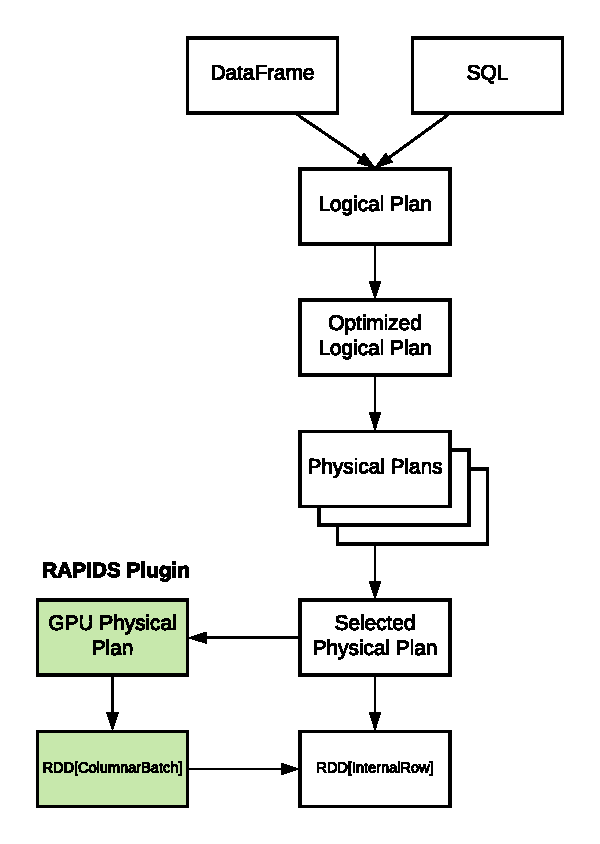
\includegraphics[scale=1]{images/04_technical_background/rapids/rapids_catalyst_optimization_process}
\caption{Catalyst optimization with RAPIDS accelerator for Apache Spark - Source: Authors own model, based on \cite{Mcdonald2020SparkRapids}.}
\label{fig:04_rapids_ext_query-plan}
\end{figure}
\paragraph{}\Fig{fig:04_rapids_ext_query-plan} illustrates how the RAPIDS plugin suite extends the Catalyst optimization process illustrated previously in \Fig{fig:04_spark_pr-model_catalyst_process}.
% How does the Catalyst create GPU aware plans
The Spark Catalyst optimizer identifies operators in a query plan that are supported by the RAPIDS \hyperlink{abbr:api}{API}. To execute the query plan, these operators can be scheduled on a \hyperlink{abbr:gpu}{GPU} within the Spark cluster \cite{Mcdonald2020SparkRapids}. If the RAPIDS \hyperlink{abbr:api}{APIs} do not support operators, a physical plan for \hyperlink{abbr:cpu}{CPUs} is generated by the Catalyst optimizer to execute \hyperlink{abbr:rdd}{RDD} operations \cite{Mcdonald2020SparkRapids}.


\subsection{GPU Accelerated Machine Learning with XGBoost}
% SHort Intro
RAPIDS accelerates SparkSQL operations and operations on a DataFrame. Additionally, RAPIDS aims to accelerate the training process of machine learning models.
% Only XGBoost
Currently, RAPIDS only supports \hyperlink{abbr:gpu}{GPU}-acceleration for Extreme Gradient Boosting (\hyperlink{abbr:xgboost}{XGBoost}) in SparkML \cite{Mcdonald2020SparkRapids}.


% Whats XGBoost
\hyperlink{abbr:xgboost}{XGBoost} is a scalable, distributed gradient-boosted machine learning library. It tries to solve many data science problems, by implementing \hyperlink{abbr:ml}{ML} algorithms using the gradient boosting technique.
% XGBoost4j-Spark
With the XGBoost4j-Spark\footnote{XGBoost Documentation - \url{https://xgboost.readthedocs.io/en/latest/jvm/xgboost4j_spark_tutorial.html} (Accessed: 2021-01-28)} library, \hyperlink{abbr:xgboost}{XGBoost} integrates into the Apache SparkML library \cite{XGBoost2021Docs}. 


\subsection{Installation Requirements for Apache Spark Standalone Mode}
\label{subsec:04_rapids_req}
The RAPIDS accelerator for Apache Spark is available for a standalone mode Apache Spark cluster. To operate efficiently, the following requirements need to be installed on all Apache Spark nodes in the cluster \cite{SparkRapids2020Docs}:
% requirements
\begin{itemize}
\item Java Runtime Environment (\hyperlink{abbr:jre}{JRE})
\item NVIDIA \hyperlink{abbr:gpu}{GPU} driver
\item \hyperlink{abbr:cuda}{CUDA} Toolkit\footnote{CUDA Toolkit - \url{https://developer.nvidia.com/cuda-toolkit} (Accessed: 2021-01-01)}
\item RAPIDS accelerator for Apache Spark Java library
\item cuDF Java library that is supported by the RAPIDS accelerator Java library, and the installed \hyperlink{abbr:cuda}{CUDA} toolkit
\item XGBoost4j Java library
\item XGBoost4j-Spark Java library
\item \hyperlink{abbr:gpu}{GPU} resource discovery script
\end{itemize}


% ===========================================
% ===========================================
% PROMETHEUS
% ===========================================
% ===========================================
\section{Prometheus}
\label{sec:04_prom}
% What is Prometheus
Prometheus is an open-source monitoring and alerting system \cite{Prom2020Docs}.
% Time-series format + PromQL
To collect and store data, Prometheus supports a multi-dimensional key-value pair based data model, according to \SubSec{subsec:02_monitoring_db_multi-model}, which can be analyzed by using the PromQL query language \cite{Pandey2020Monitoring}.
% SHort PromQL
PromQL is a functional query language for selecting and aggregating time-series data in real-time \cite{Prom2020Docs}.
% Pull-based approach
Prometheus follows the pull-based approach described in \SubSec{subsec:02_monitoring_push-pull} to scrape metrics from hosts and services \cite{Bastos2019Prom}.


\subsection{Prometheus Architecture}
\label{sec:04_prom_arch}
% Architecture image
\begin{figure}[h]
\centering
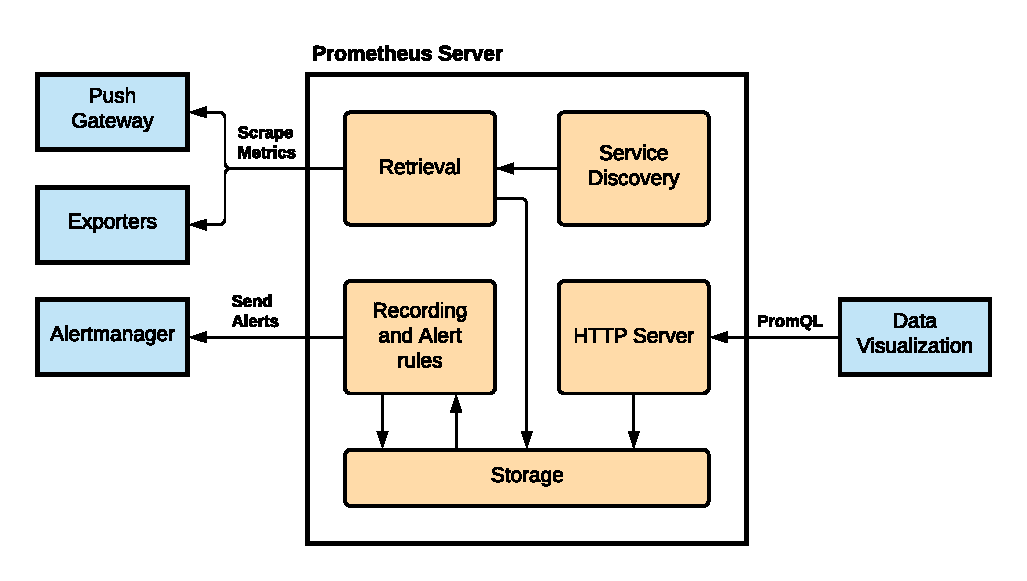
\includegraphics[scale=0.8]{images/04_technical_background/prometheus/prometheus_architecture}
\caption{Prometheus high-level architecture - Source: Authors own model, based on \cite{Prom2020Docs, Brazil2018Prom}.}
\label{fig:prom_architecture}
\end{figure}

% High level architecture
\Fig{fig:prom_architecture} illustrates the high-level architecture of Prometheus.
% Description of components
The Prometheus ecosystem provides multiple components, which can be optional, depending on the environment's monitoring needs \cite{Bastos2019Prom}. The main components of a Prometheus system are Prometheus Server, Alertmanager, service discovery, exporters, Push Gateway, and data visualization \cite{Prom2020Docs}.

\subsubsection{Prometheus Server}
% SHort intro
The Prometheus server is the main component of a Prometheus system. It is responsible for collecting metrics as time-series data from targets and stores the collected data in the built-in \hyperlink{abbr:tsdb}{TSDB} \cite{Bastos2019Prom}. Prometheus uses the concept of scraping to collect metrics from a target. A target host has to expose an endpoint to make metrics available in the Prometheus data format \cite{Pandey2020Monitoring}. Additionally, the Prometheus server triggers alerts to the Alertmanager if a configured condition becomes true \cite{Prom2020Docs}.
% The figure
The core components of the Prometheus server, as illustrated in \Fig{fig:prom_architecture}, are the following:

\begin{itemize}
% Service discovery
\item Service Discovery:
As being mentioned before, Prometheus follows a pull-based approach to fetch metrics from a target. To know about all targets, Prometheus needs a list of the corresponding hosts. The service discovery manages the complexity of maintaining a list of hosts manually in a changing infrastructure \cite{Bastos2019Prom}. Therefore, Prometheus is able to notice targets that are not responding \cite{Brazil2018Prom}.

% Retrieval
\item Retrieval:
Prometheus sends an Hypertext Transfer Protocol (\hyperlink{abbr:http}{HTTP}) request to each target to scrape metrics. The request is sent each interval, which can be set in the configuration \cite{Brazil2018Prom}.

% HTTP API
\item \hyperlink{abbr:http}{HTTP} \hyperlink{abbr:api}{API}:
Prometheus provides an \hyperlink{abbr:http}{HTTP} \hyperlink{abbr:api}{API}. This \hyperlink{abbr:api}{API} can be used to request raw data and evaluate PromQL queries.
A data visualization tool can use this \hyperlink{abbr:api}{API} to create visualizations of the requested metrics \cite{Brazil2018Prom}.

% Recording rules and alerts
\item Recording and alert rules:
Recording rules enable to precompute frequently needed or compute-intensive PromQL expressions. The result will be saved as a set of time-series in the local storage. This enables to query a recording rule at a much faster speed than the original PromQL expression \cite{Brazil2018Prom, Prom2020Docs}.

Alert rules define conditions based on PromQL expressions. If a condition becomes true, an alert will be sent to an external service \cite{Prom2020Docs}.

% Storage
\item Storage:
Received data is stored in a custom highly efficient format on a local on-disk time-series database \cite{Prom2020Docs}. Prometheus does not offer a solution for distributed storage across a cluster of machines \cite{Brazil2018Prom}.
\end{itemize}


\subsubsection{Optional Components}
The Prometheus ecosystem offers a set of optional components and can be activated depending on the monitoring needs.
The optional components illustrated in \Fig{fig:prom_architecture} are the following:

\begin{itemize}
% Alertmanager
\item Alertmanager:
If an alerting rule becomes true, the Prometheus server generates an alert and pushes it to the Alertmanager. The Alertmanager generates notifications from the received alerts. A notification can take multiple forms like emails or chat messages. Webhooks can be implemented to trigger custom notifications \cite{Bastos2019Prom}.

% Exporters
\item Exporters:
If an application does not support an endpoint for Prometheus, an exporter can be used to fetch metrics and make them available to the Prometheus server. An exporter is a monitoring agent running on a target host that fetches metrics from the host and exports them to the Prometheus server \cite{Pandey2020Monitoring}.

% Push Gateway
\item Push Gateway:
If a target is not designed to be scraped, metrics can be pushed against the Push Gateway \cite{Prom2020Docs}. The Push Gateway converts the data into the Prometheus data format and passes them to the Prometheus server \cite{Pandey2020Monitoring}.

% Data vis
\item Data Visualisation:
Prometheus supports various visualization tools, such as its built-in visualization or third-party tools. One of the widely used tools for this occasion is Grafana\footnote{Grafana: The open observability platform - \url{https://grafana.com/} (Accessed: 2021-01-19)}.
\end{itemize}


\subsection{Prometheus Configuration}
\label{sec:04_prom_config}
% Short intro
Prometheus scraping jobs and rules can be configured using external \hyperlink{abbr:yml}{YAML} files \cite{Prom2020Docs}.
% Explain listing
\Lst{lst:04_prom_config_example} shows a valid configuration file example.
% global section
In the \texttt{global} configuration section, default values can be set.
% scrape_configs
Targets are defined in the \texttt{scrape\_configs} section. Each target is defined as a scrape job with a unique name.  A target can be defined statically using the \texttt{static\_configs} parameter or dynamically using the available service discovery mechanisms \cite{Prom2020Docs}.
% rules
Rules have to be configured in a separate \hyperlink{abbr:yml}{YAML} file. To load rules into Prometheus, the file path has to be set in the \texttt{rule\_files} parameter.

% config file example
\begin{lstlisting}[label=lst:04_prom_config_example, caption=Prometheus configuration file example]
global:
  scrape_interval: 5s

scrape_configs:
  - job_name: cadvisor
    static_configs:
      - targets: ["cadvisor:8080"]
        labels:
          group: "cadvisor"
          
rule_files:
  - "/etc/prometheus/recording_rules.yml"
\end{lstlisting}

% rules example
\Lst{lst:04_prom_config_rule-example} shows a configuration example of a recording rule which are defined in groups. 
% Rule config
Each rule is defined by a name and a valid PromQL expression \cite{Prom2020Docs}.

% Recording rule example
\begin{lstlisting}[label=lst:04_prom_config_rule-example, caption=Prometheus rules configuration file example]
groups:
  - name: http_requests
     - record: job:http_inprogress_requests:sum
       expr: sum by (job) (http_inprogress_requests)
\end{lstlisting}


% ===========================================
% ===========================================
% CADVISOR
% ===========================================
% ===========================================
\section{cAdvisor}
% What is cAdvisor
Container Advisor (cAdvisor) is a running daemon that collects, aggregates, analyses, and exposes performance metrics from running containers.
% How to run
It has native support and is deployed as a Docker container.
% How it collects
cAdvisor collects metrics from the container daemon and Linux cgroups and exposes them in the Prometheus file format \cite{Bastos2019Prom, cadvisor2020Docs}.


% ===========================================
% ===========================================
% DCGM-EXPORTER
% ===========================================
% ===========================================
\section{DCGM-Exporter}
% Intro
DCGM-Exporter is a monitoring agent for collecting health and performance metrics from NVIDIA \hyperlink{abbr:gpu}{GPUs}. It exports collected metrics in the Prometheus format and makes them available using an \hyperlink{abbr:http}{HTTP} endpoint \footnote{DCGM-Exporter - \url{https://ngc.nvidia.com/catalog/containers/nvidia:k8s:dcgm-exporter} (Accessed: 2021-02-12)}.
% DCGM
The DCGM-Exporter is built on top of the NVIDIA Data Center GPU Manager (\hyperlink{abbr:dcgm}{DCGM}), a tool-suite for managing and monitoring NVIDIA \hyperlink{abbr:gpu}{GPUs} in a cluster \footnote{NVIDIA DCGM - \url{https://developer.nvidia.com/dcgm} (Accessed: 2021-02-12)}.
%
It can be deployed to a cluster using a Docker container. \Lst{lst:04_dcgm_deploy} provides an example of deploying the DCGM-Exporter using a Docker container. As a requirement, the NVIDIA Container Toolkit\footnote{NVIDIA Cloud Native technologies documentation - \url{https://docs.nvidia.com/datacenter/cloud-native/container-toolkit/overview.html} (Accessed: 2021-01-28)} has to be installed on the host.
\begin{lstlisting}[label=lst:04_dcgm_deploy, caption=DCGM-Exporter deployment using a Docker container, language=bash, numbers=none]
$ docker run -d --rm \
    -p 9400:9400 \
    --runtime nvidia \
    nvidia/dcgm-exporter:2.0.13-2.1.1-ubuntu18.04
\end{lstlisting}


% ===========================================
% ===========================================
% Gitlab CI/CD
% ===========================================
% ===========================================
\section{GitLab CI/CD}
\label{sec:04_background_gitlab}
GitLab CI/CD is a tool integrated into the GitLab platform that enables Continuous Integration (\hyperlink{abbr:ci}{CI}) and Continuous Delivery/Deployment (\hyperlink{abbr:cd}{CD}) for software development.
% Gitlab platform
The GitLab platform integrates many development features like Git repository management and \hyperlink{abbr:ci}{CI}/\hyperlink{abbr:cd}{CD}.
% How it works
By pushing code changes to the codebase, GitLab CI/CD executes a pipeline of scripts to automate the software development cycle's \hyperlink{abbr:ci}{CI} and \hyperlink{abbr:cd}{CD} processes.
% CI
A \hyperlink{abbr:ci}{CI} pipeline consists of scripts that build, test, and validate the updated codebase.
% CD
A \hyperlink{abbr:cd}{CD} pipeline is responsible for deploying the application for production after the \hyperlink{abbr:ci}{CI} pipeline was executed successfully.
% Summary
Adding \hyperlink{abbr:ci}{CI}/\hyperlink{abbr:cd}{CD} pipelines to the software development cycle of an application allows to catch bugs and errors early. This ensures that an application deployed to production will conform to established standards \cite{Gitlab2020Docs}.

\subsection{CI/CD Pipeline}
\label{subsec:04_background_gitlab_pipeline}
The fundamental component of GitLab CI/CD is called a pipeline. Pipelines perform based on conditions. A condition might be a push to the main branch or a specific branch of the repository \cite{Gitlab2020Docs}. A pipeline comprises of two components:

\begin{itemize}
\item Stages: A stage consists of one or multiple jobs that run in parallel. Furthermore, a stage defines how jobs will be executed. For example, a build stage only performs after a test stage has performed successfully \cite{Gitlab2020Docs}.

\item Jobs: Jobs are responsible for performing the scripts defined by administrators. The scripts define necessary actions. For example compiling the source code or performing tests \cite{Gitlab2020Docs}.
\end{itemize}


% How to configurate a pipeline (.gitlab-ci.yml)
GitLab CI/CD is configured by a \texttt{.gitlab-ci.yml} file. The file must be located in the repository root directory.
% What does this file
The configuration file will create a pipeline that performs after a push to the repository \cite{Gitlab2020Docs}.


\subsection{Example of a Basic CI/CD Pipeline Architecture}
\label{subsec:04_background_gitlab_basic-pipeline}
\begin{figure}[h]
\centering
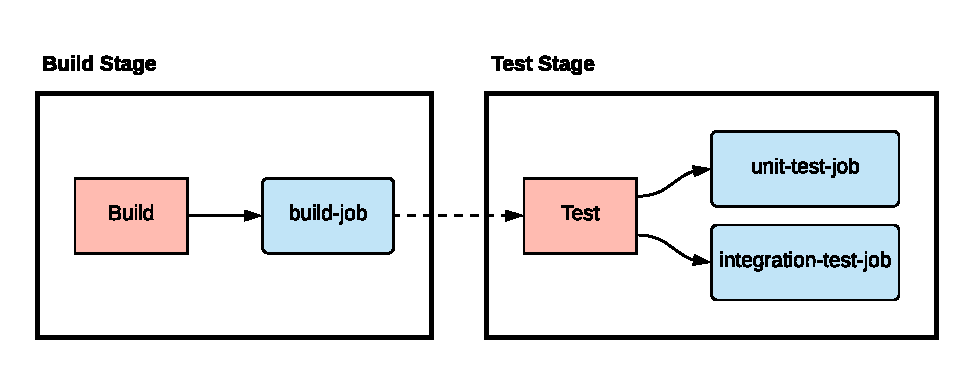
\includegraphics[scale=0.8]{images/04_technical_background/gitlab/basic_pipeline}
\caption{Basic architecture of a GitLab CI/CD pipeline - Source: Authors own model, based on \cite{Gitlab2020Docs}.}
\label{fig:04_gitlab_pipeline_basic_arch}
\end{figure}

% Explain figure
\Fig{fig:04_gitlab_pipeline_basic_arch} illustrates an architecture of a basic \hyperlink{abbr:ci}{CI}/\hyperlink{abbr:cd}{CD} pipeline.
% Two stages
The pipeline consists of a build and a test stage, which are performed in order. The test stage will only be performed after the build stage was successful.
% Build stage
The build stage consists of a single job named \textit{build-job}, which is executed first after a change is pushed to the repository.
% Test stage
The test stage consists of two jobs called \textit{unit-test-job} and \textit{integration-test-job}. If a stage consists of more than one job, then all jobs are executed in parallel when the stage is triggered.


% Example config

% Explain example
\Lst{lst:04_gitlab_pipeline_basic_config-example} provides the configuration for the basic pipeline example.
% Shell script
Each job executes a shell script to perform the desired actions. The shell scripts have to be located in the source code repository.
\newpage
% The example
\begin{lstlisting}[label=lst:04_gitlab_pipeline_basic_config-example, caption=Example of a \texttt{.gitlab-ci.yml} configuration file]
stages:
  - build
  - test

build-job:
  stage: build
  script:
    - build_software.sh

unit-test-job:
  stage: test
  script:
    - run_unit_tests.sh
    
integration-test-job:
  stage: test
  script:
    - run_integration_tests.sh
\end{lstlisting}


\subsection{Job Execution}
\label{sec:04_background_gitlab_job}
% Runner pick up jobs
GitLab runners will perform jobs that are defined in the configuration file. 
% What is runner
A GitLab runner is a lightweight and highly scalable application that runs on a server and performs one or multiple executors. Furthermore, it performs given jobs in its environment and responds the result back to the GitLab instance.
% WHat is an executor
An executor provides the environment where jobs are executed in. GitLab runner provides multiple executors, such as the Docker executor that connects to the underlying Docker engine. In addition, the Docker executor performs a job in a separate and isolated Docker container.
% Runner config
GitLab runner can be set up for specific projects or be available to all projects on the GitLab platform \cite{Gitlab2020Docs}.


% ===========================================
% ===========================================
% Scaling heat
% ===========================================
% ===========================================
\newpage
\section{Scaling Heat}
\label{sec:04_scal-heat}
% Intro
The Scaling Heat algorithm is a decision making algorithm to determine if a scaling action is necessary.
% Authors and why
It was introduced by Barna et al. \cite{Barna2017ElasticContainerApps} to overcome issues of traditional recurrence factor algorithms \cite{Barna2017ElasticContainerApps}.


\subsection{Recurrence Factor}
% Why recurrence factor
\paragraph{}
In an autonomic computing environment, a scaling decision is made in each interval after data has been retrieved from the monitoring system (see \Sec{sec:02_ac} for the autonomic computing architecture). 
% Performance spikes
Sudden performance spikes can occur, and the decision algorithm performs unnecessary scaling actions.
% The problem
These unnecessary scaling actions can have a negative impact on the overall computing performance.
% The recurrence factor
To overcome this issue, a recurrence factor needs to be introduced to the decision making algorithm.
% What it does
With a recurrence factor ($n$), a scaling action is only performed until a performance threshold is violated $n$ times \cite{Barna2017ElasticContainerApps}.


% Problems of traditional recurrence factor algos
\paragraph{}Traditional recurrence factor algorithms require violations to occur regularly. If a performance violation of the opposite direction occurs, the algorithm can get stuck in the violation process. Then, no scaling actions are performed \cite{Barna2017ElasticContainerApps}.


\subsection{Scaling Heat Algorithm Concept}
\label{sec:04_background_scaling-heat}
% Describe the concept
\paragraph{}\Alg{alg:04_scal-heat_concept_algo} introduces the Scaling Heat algorithm.
% The base
The algorithm is based on a concept called \textit{heat}. The value of heat indicates if a scaling action of adding or removing components is necessary.
% Violations
If the given utilization of a performance metric violates the upper threshold, the heat value will increase. Violations of the lower threshold will cause a decrease, respectively.
% Recurrence
When the heat reaches the recurrence factor $n$, positive for adding and negative for removing nodes, a scaling action is executed.
% Reset
After executing a scaling action, the heat value is reset to 0 \cite{Barna2017ElasticContainerApps}.
% The algorithm
\begin{algorithm}[H]
\SetKwInput{KwInput}{Input}
\SetKwInput{KwOutput}{Output}
\SetAlgoLined
\KwInput{$utilization$ - The retrieved utilization for a performance metric}
\KwInput{$lower\_threshold$ and $upper\_threshold$ - Range limit of the performance metric}
\KwInput{$heat$ - Current heat value of a performance metric. Indicating if a scaling action is necessary}
\KwOutput{$heat$ - New heat value for the next iteration}
\uIf{$utilization \geq upper\_threshold$}{
   \tcp{cluster overload}
   \uIf{$heat < 0$}{
     \tcp{reset heat for removal}
     $heat \leftarrow 0$\;
   }
   $heat \leftarrow heat + 1$\;
   }
   \uElseIf{$utilization \leq lower\_threshold$}{
     \tcp{cluster overload}
     \uIf{$heat > 0$}{
       \tcp{reset heat for adding}
       $heat \leftarrow 0$\;
     }
     $heat \leftarrow heat - 1$\;
   }  
   \Else{
   \tcp{utilization is within threshold range}
   \tcp{move heat towards 0}
   \uIf{$heat > 0$}{
      $heat \leftarrow heat - 1$\;
   }
   \uElseIf{$heat < 0$}{
      $heat \leftarrow heat + 1$\;   
   }
  }
\uIf{$heat = n$}{
Perform a scale-out action\;
$heat \leftarrow 0$\;
}
\uElseIf{$heat = -n$}{
Perform a scale-in action\;
$heat \leftarrow 0$\;
}
\Return{heat}
\caption{Scaling Heat decision making algorithm\cite{Barna2017ElasticContainerApps}}
\label{alg:04_scal-heat_concept_algo}
\end{algorithm}


% ===========================================
% ===========================================
% KHP
% ===========================================
% ===========================================
\newpage
\section{Kubernetes Horizontal Pod Autoscaler}
\label{sec:04_background_khpa}
\paragraph{}
% Short intro
Kubernetes Horizontal Pod Autoscaler (\hyperlink{abbr:khpa}{KHPA}) is an auto-scaling algorithm used in Kubernetes, which is an orchestration tool that allows to create and deploy units called Pods. A Pod is a running process on a cluster that encapsulates an application.
% What
\hyperlink{abbr:khpa}{KHPA} scales the number of replicas per Pod based on the utilization of performance metrics.
% Interval
The algorithm is based on a control loop. Each $n$ seconds, the algorithm gathers performance metrics and computes the target number of replicas to achieve the desired utilization of a performance metric \cite{Casalicchio2017AutoScaleCont}.


% Support for multiple metrics
The algorithm computes the number of replicas for a single performance metric. If a scaling action depends on multiple performance metrics, the number of replicas has to be computed for each performance metric. The largest number of replicas is used as the target number of replicas \cite{Kubernetes2021Docs}.


\paragraph{}
\hyperlink{abbr:khpa}{KHPA} takes as input the number of active replicas for a pod ($active\_replicas$), the utilization of the performance metric of each replica ($pod\_utilization$), and the target utilization of the performance metric ($target\_utilization$).
% Intro formula
The formula to compute the target number of pods $P$ is defined by \cite{Kubernetes2021Docs}:
% The formula
\begin{equation}
P = \left \lceil active\_replicas \times \left ( \frac{\sum pod\_utilization}{target\_utilization} \right ) \right \rceil
\label{eq:04_background_khpa_equation}
\end{equation}


\chapter{Conceptual Design}
\label{chap:05_design}
%
\todo{Describe Chapter}


% ===========================================
% ===========================================
\section{Design Restrictions}
\label{sec:05_restrictions}
The design of the computing environment will be restricted by several points. These factors are given because of technological choices and requirements from up there.

\begin{itemize}
\item \textbf{Running on a NVIDIA DGX A100\footnote{The Universal System for AI Infrastructure - \url{https://www.nvidia.com/en-us/data-center/dgx-a100/}}:} The environment will run on a NVIDIA DGX A100 workstation. The workstation has 80 CPUs and 8 GPUs installed. For this computing environment, 2 GPUs will be available.

\item \textbf{Apache Spark for distributed computing:} Apache Spark will be used as a distributed computing framework.

\item \textbf{Python as the main programming language:} Python will be used as the main programming language for Apache Spark applications. Therefore, examples will use Python code. Configurations for the system are optimized for using Python in production.

\item GitLab as repository: sadf <- Eher implementation detail/requirement
\end{itemize}

% ===========================================
% ===========================================
\section{Automated Deployment Pipeline}
% Abstract
The objective of this thesis is to automatically submit an Apache Spark application to the Apache Spark cluster to train ML models. Therefore, the training process has to be integrated into the application development lifecycle.
% Git
The source code of an Apache Spark application is hosted on a Git repository. After each committed change on the repository, the pipeline is triggered.


% Conceptual figure
\begin{figure}[h]
\centering
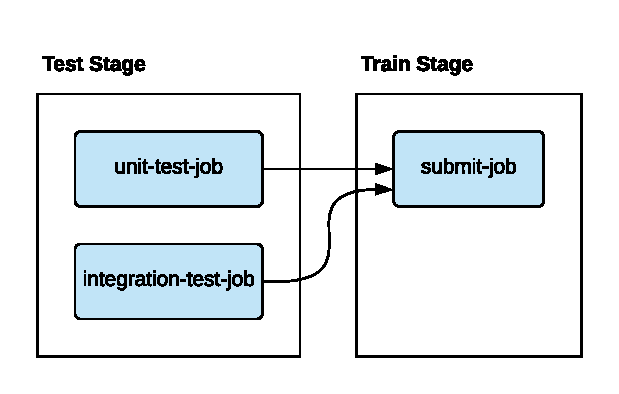
\includegraphics[scale=1]{images/05_conceptual_design/automated_deployment_pipeline/ci_cd_concept}
\caption{Automated Deployment Pipeline concept}
\label{fig:05_deployment_concept}
\end{figure}
% Short intro
\Fig{fig:05_deployment_concept} illustrates the conceptual design of the Automated Deployment Pipeline.
% The stages
The pipeline consists of two different stages:
\begin{enumerate}
\item Test stage: After the build stage has succeeded, the test stage will perform tests.
\item Train stage: If the tests have been successful, the application is submitted to the Apache Spark cluster for training.
\end{enumerate}
% No build stage
It is important to mention, that a build stage is missing in this conceptual design. The build stage includes compiling source code into a format that can be executed directly.
% Python
Python is an interpreted language and therefore no compilation is needed to execute the source code. \todo{Quelle}
% Other languages
As being mentioned in Section SPARK, Apache Spark supports different languages that Python.  For example, for Java application, a build stage is needed to compile the source code to a .jar binary, which can be submitted to the Apache Spark cluster.


\subsection{Test Stage}
% short intro
In order to detect error in an early stage, the source code has to be tested.
% responsibilities
The test stage is responsible to the the source code within a set of various tests. Tests can include:
% Tests
\begin{itemize}
\item Unit tests:
\item Integration tests:
\item End-to-end tests:
\end{itemize}
% Different jobs
For each different test, a new job in the test stage is being created. All jobs will perform in parallel after the test stage has been triggered.
% On failure
If a job has failed, the whole test stage is marked as failure and all participating developers will get a notification.


\subsection{Train Stage}
\paragraph{}
% Short intro
The train stage is responsible to submit the Apache Spark application to the Apache cluster after the test state was successful.
% How
As being mentioned in SECTION XY, an Apache Spark application will be submitted to the Apache Spark cluster by creating a spark-submit Docker container in the same Docker swarm network.
Therefore, after the train stage has been triggered a spark-submit container has to be deployed in the Apache Spark cluster to submit the latest version of the Apache Spark application.

\paragraph{}
% Same machine
To access the Apache Spark cluster Docker swarm network, the train stage has to be executed on the same machine.
% Gitlab runner
Therefore a GitLab runner performing on the machine is needed. Additionally, the GitLab runner needs access to the underlying Docker engine to deploy new container to a given network.
% Perform train stage concept
\begin{figure}[h]
\centering
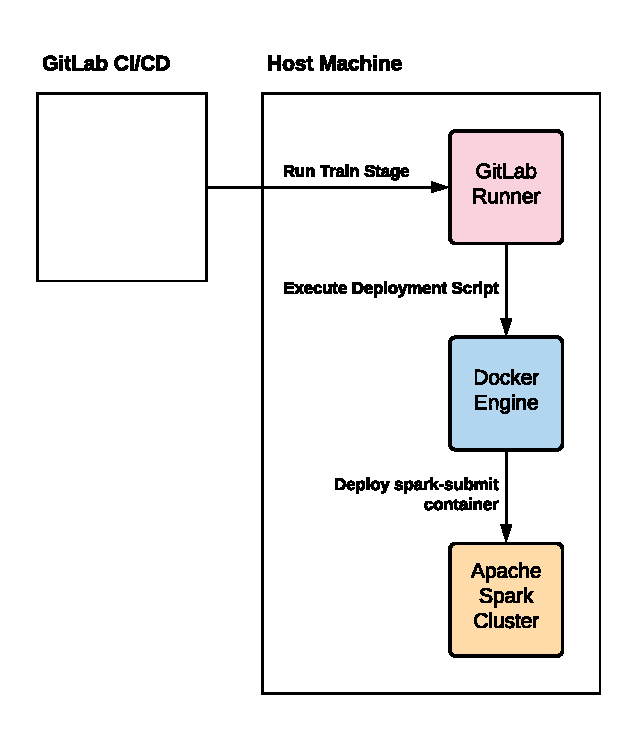
\includegraphics[scale=1]{images/05_conceptual_design/automated_deployment_pipeline/train_stage_runner}
\caption{Deployment of a spark-submit container}
\label{fig:05_deployment_train_concept}
\end{figure}
% Explain figure
\Fig{fig:05_deployment_train_concept} illustrates the steps to deploy a spark-submit container in the Apache Spark cluster swarm network.
% Runner
GitLab CI/CD performs the train stage on the GitLab runner which is running on the NVIDIA DGX machine.
% Deploy
The GitLab Runner executes the deployment script defined in the train stage.
% Deploy script
The deployment script executes Docker CLI commands to deploy a spark-submit container in the Apache Spark cluster swarm network.


% ===========================================
% ===========================================
\section{Identification of Suitable Metrics for Scaling}
% SHort intro
To scale the number of Apache Spark worker in accordance to the actively performing workload, suitable metrics to define the cluster performance have to be defined.
% Rapids enabled GPU
With the RAPIDS accelerator for Apache Spark enabled, the Apache Spark cluster is able to utilize the computing power of GPUs and CPUs to enable parallization.
% SO?
Therefore, suitable metrics to measure the performance are the overall CPU utilization across all worker and the GPU utilization of all available GPUs.
% Those are time-based utilization
These utilization metrics will be based on the time when the Aapche Spark cluster is actively performing computations.


\subsection{CPU Utilization}
% Sharing CPU cores
All Apache Spark worker run on the same machine. Therefore, all available CPU cores on the machine will be shared across each running Apache Spark worker.


% cadvisor
cAdvisor provides a performance called metric \texttt{container\_cpu\_usage\_seconds\_total}\footnote{Monitoring cAdvisor with Prometheus - \url{https://github.com/google/cadvisor/blob/master/docs/storage/prometheus.md} (Accessed: 2021-01-21)}. This metric provides the total amount of CPU seconds consumed by core per container. 
% Overall utilization
To calculate the overall CPU utilization for all Apache Spark worker, the value of the performance metric for each over a specific rate has to be summed up. Therefore, the CPU utilization ($U_{CPU}$) is defined by:

\begin{equation}
U_{CPU}=\sum_{n=1}^{ActiveWorker}container\_cpu\_usage\_seconds\_total_{n}
\label{eq:formel}
\end{equation}

\subsection{GPU Utilization}
% Number of gpus
Two GPUs on the machine are available across all Apache Spark Worker.
% The metric
The dcgm\_exporter agent provides the \texttt{bla\_bla} performance metric. This metric returns the procentual utilization per GPU.
% How to calculate
Therefore, the overall GPU utilization ($U_{GPU}$) is defined by:


The system has a fixed number of GPUs to use.
\begin{equation}
U_{GPU} = \dfrac{\sum bla\_bla}{ActiveGPUs}
\label{eq:formel}
\end{equation}


% ===========================================
% ===========================================
\section{Computing environment Architecture}

\todo{Only self-adapting -> wegen autonomic computing}

\subsection{Overall}
\label{subsec:05_arch_overall}

% Figure
\begin{figure}[h]
\centering
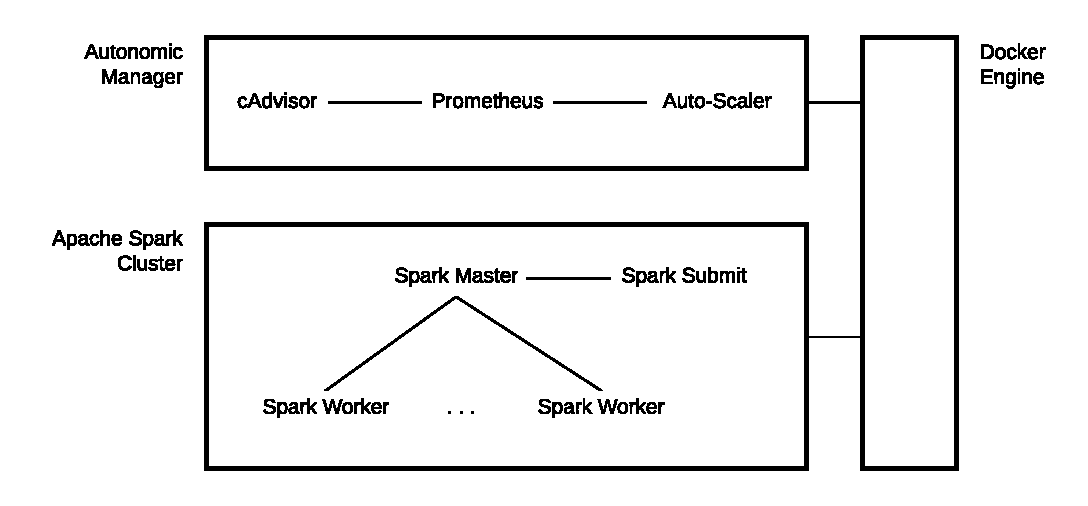
\includegraphics[scale=0.8]{images/05_conceptual_design/cluster_architecture/overall_architecture}
\caption{Overall cluster architecture - Source: Authors own model.}
\label{fig:ca-overall_architecture}
\end{figure}

\Fig{fig:ca-overall_architecture} illustrates the overall architecture with all components of the computing environment. The two main components in the environment are an Apache Spark cluster and an autonomic manager.
% The components
The autonomic manager will be implemented according to the MAPE architecture (introduced in \SubSec{subsec:02_ac_manager}). It is responsible for monitoring and auto-scaling the Apache Spark cluster. To enable distributed computing, an Apache Spark cluster will be set up to execute machine learning applications. 
% The nodes and virtualization
The autonomic manager and the Apache Spark cluster consist each of multiple nodes. Each node of a component will run as a Docker container.
% Self healing
All containers will run as services in Docker Swarm mode. As described in \SubSec{subsec:04_docker_swarm}, Docker Swarm mode will maintain a healthy state of all running containers. Therefore, the environment will enable self-healing according to the requirements of Autonomic Computing described in \Sec{sec:02_ac}.


\subsection{Apache Spark Cluster}
\label{subsec:05_arch_spark}

\todo{Why standalone -> Because most simple way; Master und worker -> Managed Resources}

\subsubsection{Master and Worker}
The Apache Spark cluster will consist of a Spark master node and a dynamic number of Spark worker nodes.
% Master
The Spark master node is responsible to distribute the application workload across available Spark worker nodes.
% Worker
A Spark worker node will execute the workload given by the master node. Each Spark worker is homogeneous. 
% Homegeneous spark worker
Homegenneosity is important to scale the number of worker nodes. To enable homogeneous nodes, each SPark worker node is a Docker container running the same Docker image. In addition, each worker is given the same computing resources. With homogeneous Spark worker nodes, each worker will respond as all other nodes.
% GPU acceleration
To enable GPU acceleration, each WORKER/MASTER will have the RAPIDS plugin installed.
% Standalone mode
The cluster will be deployed in standalone mode. To be able to run Python applications


\subsubsection{Spark Submit}
Because the Apache Spark cluster ill be executed in standalone mode, a node inside the cluster is required to run Spark applications. When a Spark application will be executed, a Spark Submit container will be deployed in the cluster. When the appliccation has finished, the container will be automatically removed.
Each app will be executed by a unique Spark Submit node.
The Spark Submit node will be deployed via the CI pipeline (SECTION XY). The prupose of this 


\subsection{Autonomic Manager}
\label{subsec:05_arch_am}

\begin{figure}[h]
\centering
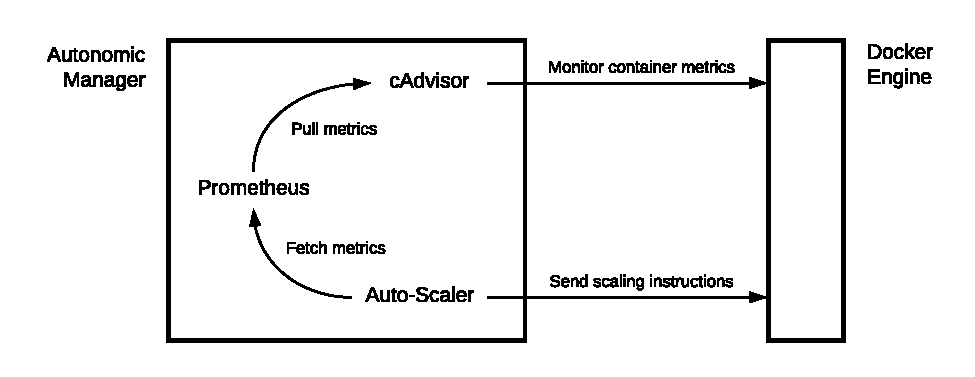
\includegraphics[scale=0.85]{images/05_conceptual_design/autonomic_manager/autonomic_manager_overview}
\caption{Autonomic manager component design - Source: Authors own model.}
\label{fig:am-design-component}
\end{figure}

% MAPE architecture
The design of the autonomic manager needs to fullfill all requirements given by the MAPE architecture (described in \SubSec{subsec:02_ac_manager}). It will be responsible to monitor the performance of Apache Spark worker nodes in the environment, analyze the metrics and plan and execute scaling actions in accordance to fullfill the performance goals.
% Figure
As illustrated in \Fig{fig:am-design-component}, the autonomic manager consists of a cAdvisor, Prometheus and Auto-Scaler node. Together, all three nodes build a complete autonomic manager in accordance to the MAPE architecture. Each node will run as a Docker container.
% Explain figure
For monitoring, cAdvisor collects metrics from all available Docker container in the computing environment. Prometheus pulls metrics from cAdvsior. The Auto-Scaler will fetch metrics from Prometheus and send scaling instructions to the Docker engine.


\subsubsection{Monitoring System}
% Why - dynamic env, requirements, etc
The design introduced in \SubSec{subsec:05_arch_overall} is a dynamic changing computing environment. To monitor this dynamic environment, a monitoring-system is needed that fullfills the requirements described in \Sec{sec:02_monitoring}.


% Gathering metrics
cAdvisors will be used as an agent to collect performance metrics from all running Docker containers in the environment.
% Store metrics
Prometheus pulls the collected performance metrics from cAdvisor and stores the data as time-series data in its database.
% Query
In addition, Prometheus provides a powerful multi-dimensional query language to aggregate and analyze the stored data.

% Collecting operational data can be challenging in a horizontally        scaling environment since the number of nodes varies over time. Any        system that automates gathering of log files from individual nodes        needs to account for this, and care needs to be taken to ensure that        logs are captured before nodes are released.


\subsubsection{Workflow}

\paragraph{} The workflow of the autonomic manager is implemented as a loop.

% Workflow
\begin{figure}[h]
\centering
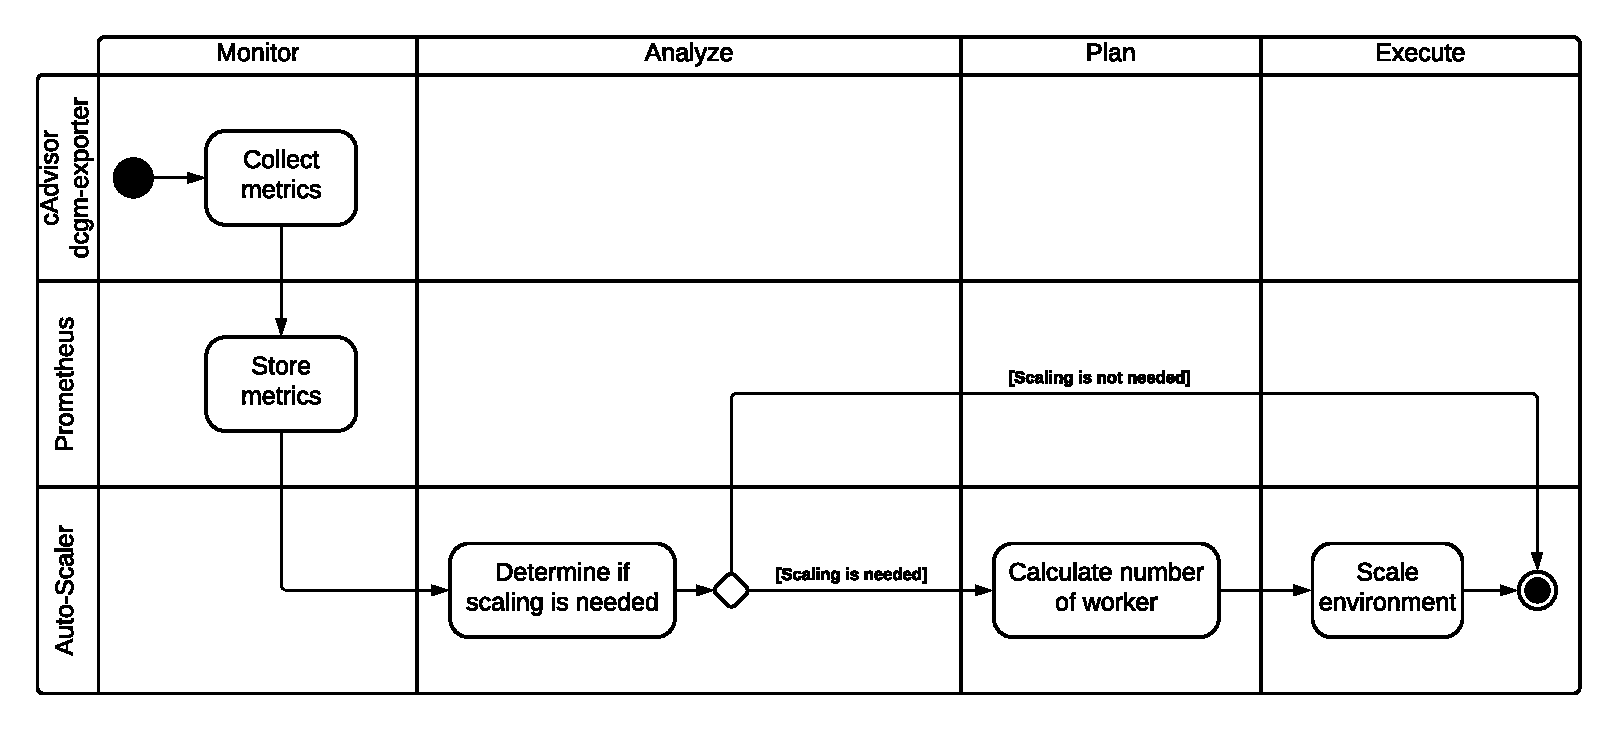
\includegraphics[scale=0.50]{images/05_conceptual_design/autonomic_manager/autonomic_manager_workflow}
\caption{UML activity model of the autonomic manager process - Source: Authors own model.}
\label{fig:am-workflow}
\end{figure}
% Explain figure
\paragraph{} \Fig{fig:am-workflow} illustrates all steps of each component of the autonomic manager process according to the MAPE architecture.


% Monitor
The workflow starts with collecting metrics in the monitor phase. cAdvisor is responsible to collect metrics from the Docker engine. After that, Prometheus stores the collected metrics as time-series data in its database.
% Analyze
Next, in the analyze phase, the Auto-Scaler needs to determine if a scaling action is needed. If scaling the Apache Spark worker nodes is not needed, the process has finished and will repeat from the beginning in the next period.
% Plan
If the performance is over- or under-utilized, a scaling action is needed. Then, the Auto-Scaler needs to determine how many Apache Spark worker nodes are needed to reach the performance goal.
% Execute
Lastly, the Auto-Scaler is responsible to send the scaling instructions to the Docker engine.


% ===========================================
% ===========================================
\section{Auto-Scaler}
\label{sec:05_auto-scaler}
% What is the Auto-Scaler
The Auto-Scaler is a component of the the Autonomic Manager and is responsible for the analyze, plan and execution phase.
% Complete autonomic manager
Together with cAdvisor and Prometheus, the Auto-Scaler builds a complete Autonomic Manager according to \SubSec{subsec:02_ac_manager}.
% control loop
In addition, the Auto-Scaler implements the control-loop which is responsible to make adjustments in the environment according to the performance.
% Communication with Prometheus
To adjust the number of Apache Spark worker in the environment, the Auto-Scaler needs to perform queries on the performance metrics stored in Prometheus.
% Analyzing
After analyzing the performance metrics, the Auto-Scaler will send instructions to adjust the number of Apache Spark worker to the Docker engine. The Docker engine tells the Swarm manager to scale the replicas of the Apache Spark service in accordance to the Auto-Scaler instructions.

\todo{HIER NOCH BILD VON SCALER WIE MIT DER MAPE ARCH; Reactive Auto-Scaler, threshold-based rules}


\subsection{Configuration}
\label{subsec:05_auto-scaler_configuration}
The Auto-Scaler needs specific configuration properties to be able to collect the correct metrics from Prometheus and deploy new Apache Spark worker container in the environment. The following are properties that have to be defined to ensure that the Auto-Scaler is able to collect meaningful metrics and scale Apache Spark worker as expected.

\subsubsection{General properties}

\begin{itemize}
\item \textbf{Interval seconds:} The number of seconds when the loop has to repeat needs to be defined.

\item \textbf{Cooldown period:} The duration in seconds,  the Auto-Scaler has to wait after a scaling action was performed.

\item \textbf{Recurrence factor:} To prevent to many scaling actions,  the autonomic manager should only execute a scaling action,  if the utilization thresholds is violated \textit{n} times.

\item \textbf{Prometheus URL:} The Auto-Scaler will fetch the configured metrics from the Prometheus REST API.
\end{itemize}

\subsubsection{Metrics}

To support to analyze multiple metrics, the user should be able to create a dynamic list if metrics. Each metric needs to have a variety of properties configured.

\begin{itemize}
\item \textbf{Target utilization:} The relative target utilization of a metrics needs to be defined to calculate the number of Spark worker to add or to remove to reach the defined goal.

\item \textbf{Utilization thresholds:} To determine if a scaling action is needed, the scaling heat algorithm needs the minimum and maximum utilization defined by an administrator.

\item \textbf{Query:} A PromQL query needs to be defined to collect the metric for all Spark Worker.
\end{itemize}

\subsubsection{Apache Spark worker properties}

\begin{itemize}
\item \textbf{Worker image:} To guarantee that each Spark worker is homogeneous, all worker container should be created with the same image.

\item \textbf{Worker network:} To establish communication between all Spark worker and the Spark master, all new Spark worker container should be in the same network.

\item \textbf{Worker thresholds:} The minimum and maximum number of concurrent Spark worker should be defined. To avoid the cold start effect, the minimum amount of worker should be 1. 

\item \textbf{Apache Spark master URI:} To distribute the workload across all Spark Worker, all Spark Worker need to communicate with the Spark master.
\end{itemize}


\subsection{Analyze}
% Short intro to analyze phase
In order to determine if a scaling-action is necessary, the Auto-Scaler has to process the collected metrics. 
% How to analyze
During each period, the Auto-scaler queries the Prometheus time-series database with the configured queries to get all needed metrics. 
% Determine if scaling is needed
After the metrics are received, the Auto-Scaler determines if a scaling action is needed using the Scaling Heat algorithm (introduced in Section AB). If scaling is not necessary, the Auto-Scaler continues to collect metrics from Prometheus.


\subsection{Plan}
% Short intro
If a scaling-action is necessary, the Auto-Scaler is responsible to plan how to scale the number of Spark worker to satisfy the defined utilization goals.
% What is a scaling plan
A scaling plan consists of instructions to add or remove Spark worker which will be send to the Docker engine.
% Calculating Spark worker
To calculate the number of Spark worker, needed to accomplish the defined target utilization, the Auto-Scaler uses the \textit{Kubernetes Horizontal Pod Auto-Scaling} algorithm. In addition, the Auto-Scaler needs to check if the estimated number of Spark worker fall bellow the minimum threshold or exceed the maximum threshold of concurrent Spark worker.


\subsection{Execute}
% Short intro
After a scaling plan has been created, the Auto-Scaler needs to send the instructions to the Docker engine.
% Cooldown
After scaling the environment, it needs time for changes to take effect. Therefore a cooldown period will be activated after each scaling action.
% Whats happens
During the cooldown period, no scaling actions will be forwarded to the Docker engine.

\chapter{Implementation}
\label{sec:06_implementation}
\todo{Describe Chapter}


% ===========================================
% ===========================================
\section{Computing Environment}


\subsection{Swarm}
Vielleicht euch einfach das ganze kapitel Swarm nennen?
- Dockerfile erläutern


\subsection{Build Script}


% ===========================================
% ===========================================
\section{Apache Spark Cluster}
The Apache Spark cluster is created in standalone mode, see SECTION AB for details. There is one Apache Spark master node, a variant number of Apache Spark worker nodes and for each running application one Apache Spark Submit node. Each node runs in an independent Docker container. The Apache Spark master and worker nodes run as services in the swarm. Each Apache Spark node container is created from a custom Docker image. To simplify the images, a base image is created where all other images can inherit from.

LISTING XY shows the instructions of the base image. The following requirements are needed for all Apache Spark node images:
\begin{itemize}
\item Use Ubuntu 16.04 as base image
\item \textbf{Install Ubuntu packages:} OpenJDK 8 and Python 3 are needed to run Apache Spark and perform Python applications.
\item Install Apache Spark
\item Add the GPU discovery script
\item Download needed \textit{.jar} files for the RAPIDS plugin
\item Set environment variables
\item Set working directory
\end{itemize}


Each node needs Apache Spark 3.1 installed. A version number of at least 3 is needed to install the NVIDIA RAPIDS plugin (see SECTION AB).


\subsection{Apache Spark Master}


\subsection{Apache Spark Worker}


\subsection{Apache Spark Submit}
- Dockerfile erklären
- Config parameter


\subsection{Building Images}


% ===========================================
% ===========================================
\section{Monitoring-System}


\subsection{cAdvisor}
- Wie ist cAdvisor erreichbar
- Screenshot von cAdvisor 


\subsection{Prometheus}
- Wie ist Prometheu errecihbar
- DIe config von prometheus dateien
- Screenshots von prometheus (target und visualisierung)



%
% WARUM NICHT GPU MIT IN DIE AUTO-SCALER METRICS?
% weil alle worker sich die GPUs teilen ...
%


% ===========================================
% ===========================================
\section{Auto-Scaler}


\subsection{Code Implementation}
- Hier auch Beispiel logs
- Dann scaling heat und KHP algos


\subsection{Configuration}
- Beispiel von der yml Datei


\subsection{Docker Image}
- Dockerfile hier erklären


% ===========================================
% ===========================================
\section{GitLab CI/CD}


\subsection{Automatic Deployment of Apache Spark Applications}
Vielleicht eher das Kapitel so nennen
- gitlab-ci.yml erklären
- Screenshot von webui output


\subsection{Image Registry}
??

































\section{General}
% BLa bla alles in Docker usw.
T create an elastic computing environment, all needed components will be run as Docker container in a Docker network.


\section{Computing environment}
% The environment will be implemented with Docker/docker-compose
To create an elastic environment Docker will be used. With docker Spark worker can be easy scaled. With docker-compose an environment can be created.
% Images used
% network (Communication)
\subsection{Monitoring}
cAdvisor will be uses to monitor metrics from the Docker engine. Prometheus collects the metrics defined in Section XY from cAdvisor and stores them in its time-series database.
% The queries
The query used for getting CPU metrics:

\begin{lstlisting}[language=SQL, caption=Python example]
SUM(SELECT BLA FROM XYZ)
\end{lstlisting}

The query used for getting GPU metrics:


\subsection{Apache Spark Images}
The are 4 different Spark images:

1. Spark-Base
2. Spark-Master
3. Spark-Worker
4. Spark-Submit

Spark-Base is the foundation image for all other Spark images. Spark-Master is the image for the master node. Spark-Worker is the image for all SPark worker nodes. With Spark-Submit, a application will be submitted, the container runs as long as the application runs and exits after the execution automatically. Spark-Submit is used, because Cluster runs in Standalaone mode. Python cann submit cannot run in cluster mode QUELLE SPark.

\subsection{GPU Acceleration}

NVIDIA RAPIDS will be used as the plugin for GPU acceleration.



\section{Auto-Scaler}
The Auto-Scaler consists of a Python module which implements the logic for control-loop and a own Docker image.
% Is implemented in python
The Auto-Scaler is implemented in the Python programming language.
% Is its own Docker image
The Auto-Scaler module will be executed in an individual Docker image.
% UML diagram

\subsection{Configuration}
All configuration properties defined in the concept of the Auto-Scaler in SECTION A will be defined in a YAML file.
% As a cmd-line argument
To set the configuration properties, the configuration file needs to be set as a command-line argument.
% File example

\subsection{Control-Loop}
Control-Loop of the Auto-Scaler implements the Analyze, Plan, and Execute phase of the MAPE architecture.

\subsubsection{Analyze}
% Scaling Heat
Scaling Heat algorithm will be used to estimate if a scaling action is necessary.

\subsubsection{Plan}
% KHPA
The KHPA algorithm will be used to calculate how many worker are needed to reach the target utilization. Since we have two different metrics, the highest number of running worker will be used KUBERNETES QUELLE.

\subsubsection{Execute}
% Python Docker SDK
Via the Python Docker SDK new container will be spawned in the network.
% Check if worker is busy
If worker need to be removed, it is necessary to check if the worker are running any applications at the moment. Spark provides a REST API to check this.
% Cooldown
After a scaling action has been performed, a cooldown period will be applied so all nodes can relax.



\section{Automated Deployment}
Hier die CI/CD von gitlab.

\chapter{Evaluation}
\label{chap:07_evaluation}

In this chapter, the implementation of \Chap{chap:06_implementation} is evaluated in various experiments. Furthermore, the experimental results are discussed.

\section{Experimental Environment}
%
The experiments are conducted on the DGX introduced in \Sec{sec:06_env}.
% 2 GPUs
As for the implementation, 2 GPUs have been available for the experiments.


% ===========================================
% ===========================================
\section{Experiments}
% Intro
The performance of the computing environment is measured on two widely used machine learning algorithms.
% Explain
In both experiments, a machine learning model is trained on the computing environment using Apache Spark. Furthermore, each benchmark is evaluated using three different configurations:
\begin{enumerate}
\item Using a static number of CPU-only Apache Spark workers
\item Using a static number of GPU-accelerated Apache Spark workers
\item Dynamically scaling the replicas of CPU-only Apache Spark workers using the \textit{Auto-Scaler}
\end{enumerate}
% 10 times
For each benchmark configuration, the experiment is conducted 10 times. The spark-job execution-time mean value over all 10 iterations per experiment is used as result.
% DIfference between GPU and CPU
The performance difference between GPU accelerated worker nodes and CPU-only worker nodes is explored using a CPU-only, and a GPU-only version of the benchmark implementation.

\paragraph{}
% Why no auto gpu
The \textit{Auto-Scaler} is not evaluated using GPU-accelerated worker nodes. As mentioned, for this experiment only 2 GPUs are available. The RAPIDS plugin allocates a GPU exclusively for each executor. When the \textit{Auto-Scaler} creates a new worker node, the worker allocates a random available GPU.
% Live system
However, the host machine is a live system and it is not possible to allocate a random GPU which may be in use by another application. Furthermore, the \textit{Auto-Scaler} does not support to allocate a specific GPU for each newly created worker. An approach to overcome this problem is introduced in \Sec{subsec:08_outlook_gpus}.

\paragraph{}
% The algorithm
The two benchmarks to evaluate the performance are:
\begin{itemize}
\item XGBoost classification model using the \textit{Fannie Mae’s Single-Family Historical Loan Performance Dataset}\footnote{Downloaded from: \url{https://docs.rapids.ai/datasets/mortgage-data} (Accessed: 2021-02-06)}\cite{Fannie2021Mortgage}

\item XGBoost regression model using a Taxi fare dataset\footnote{The Taxi dataset is available at: \url{https://github.com/NVIDIA/spark-xgboost-examples/tree/spark-3} (Accessed: 2021-02-06)}
\end{itemize}
% Source
The source code and the dataset used in these experiments are available on Github on the \textit{spark-xgboost-examples}\footnote{spark-xgboost-examples - \url{https://github.com/NVIDIA/spark-xgboost-examples/tree/spark-3} (Accessed: 2021-02-06)} repository from NVIDIA.
% The two diff impl conf
The repository provides a \textit{mortgage} and a \textit{taxi} application. Both applications provide a CPU and a GPU configuration.

% supervised
Classification and regression algorithms are supervised machine learning algorithms.
% whats supervised
The goal of supervised machine learning algorithms is to train a model by finding patterns in labelled data. Then, the model is used to predict labels on new data based on the learned labels.
% Classification
The classification algorithm identifies the category of a label.
% Regression
A regression algorithm predicts a continuous numeric value \cite{Mcdonald2020SparkRapids}.


% ===========================================
% ===========================================
\section{Static Worker CPU only}
\label{sec:07_static}
% Intro
The first experiment is conducted using a fixed number of CPU-only Apache Spark workers to evaluate the performance of both benchmarks.
% Appendix
The performance for each iteration is available at \Section{sec:appendix_eval}.
% results
\begin{figure}[h]
\centering
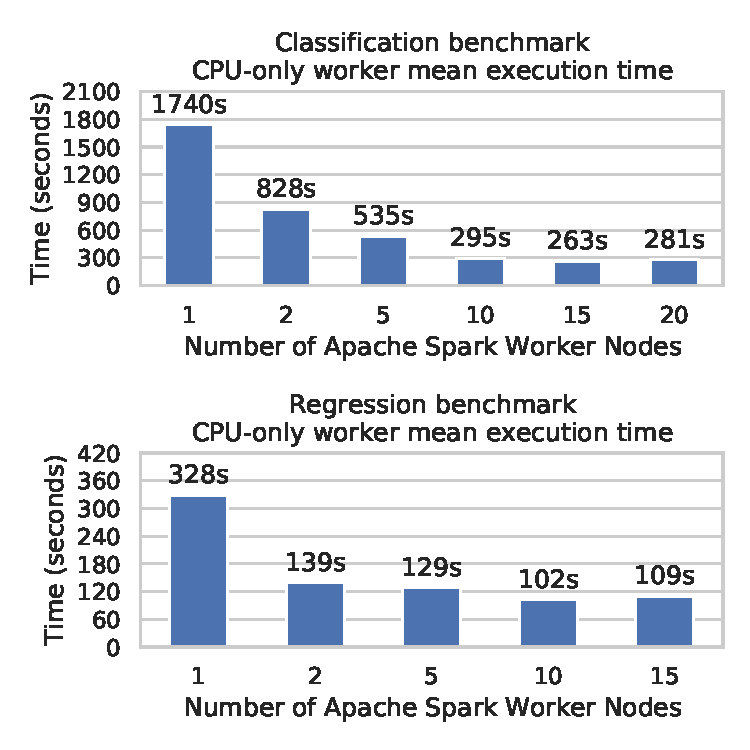
\includegraphics[scale=0.9]{images/07_evaluation/overall_cpu}
\caption{Mean execution time using CPU-only worker nodes}
\label{fig:07_static_results}
\end{figure}
% Explain fig
\Fig{fig:07_static_results} illustrates the mean execution time for both benchmarks.

\paragraph{}
% best results
The best performance for the classification benchmark was achieved with 247 seconds using 30 workers with an improvement of 7.04x in comparison to 1 worker. The regression benchmark achieved best with 102 seconds using 10 workers. The execution has an improvement of 3.21x in comparison to 1 worker. In addition, the regression benchmark achieved an execution time of 102 seconds by using 30 workers as well. However, using 10 workers is considered the best result for the regression benchmark because less workers have been used.

\paragraph{}
% The improvement curve
For the classification benchmark, the execution time had no significant improvement from 15 workers. Using 20 workers increased the execution time by 18 seconds. Using 35 workers improved the execution time by only 5 seconds in comparison to 15 workers.
% regression
The regression benchmark shows a similar result. As mentioned, the best result was achieved with 10 workers. The same results was achieved with 30 workers. Furthermore, using 35 workers increased the best performance by 7 seconds.


% and?
This result shows that over-provisioning the Apache Spark cluster by adding more workers from a certain number of workers can have a negative impact on the performance.


% ===========================================
% ===========================================
\section{GPU Acceleration}
% Intro
The impact of GPU-accelerated Apache Spark worker nodes for both benchmarks have been evaluated using 2 configurations: Using 1 GPU accelerated worker node, and using 2 GPU accelerated worker nodes.
%
The performance for each GPU experiment is available at ANHANG A.
% vs figure
\begin{figure}[h]
\centering
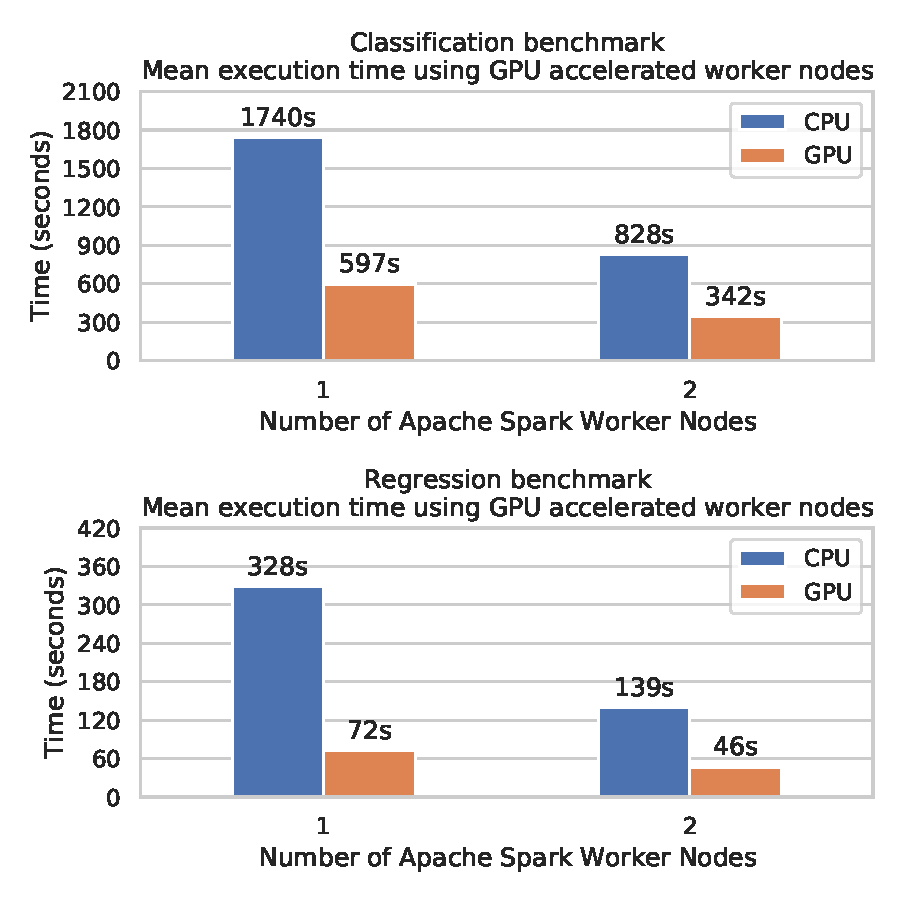
\includegraphics[scale=0.9]{images/07_evaluation/overall_cpu_vs_gpu}
\caption{Mean execution time of GPU-accelerated worker nodes vs. Mean execution time of CPU-only worker nodes}
\label{fig:07_gpu_results}
\end{figure}
% Explain results
The results of the experiment are illustrated in \Fig{fig:07_gpu_results}.
% vs
The mean execution time using GPU accelerated worker nodes are plotted against the mean execution time using CPU-only worker nodes.
% overall
Overall, GPU accelerated worker nodes significantly outperformed the equivalent number of CPU-only worker nodes.
% classification
For the classification benchmark, the best execution-time was achieved using 2 GPU-accelerated worker nodes with 342 seconds in comparison to 828 seconds using 1 CPU-only worker node. This an 2.42x improvement. Using 1 GPU-accelerated worker node achieved an improvement of 2.91x with 597 seconds in comparison to 1 CPU-only worker node with 1740 seconds.
% regression
The regression benchmark achieved best with 2 GPU-accelerated worker nodes needing 342 seconds in comparison of 2 CPU-only worker nodes needing 828 seconds. Therefore, using 2 GPU-accelerated worker nodes achieved an improvement of 3.02x. Using 1 GPU-accelerated worker node achieved an improvement of 4.55x in comparison to 1 CPU-only worker node.

\paragraph{}
% The table
\Tab{table:07_gpu_overall_results} shows the overall results by comparing the CPU and GPU results for each benchmark.
% GPU outperforms
Overall, GPU-accelerated worker nodes were able to outperform their CPU-only equivalent.
% classification
However, for the classification benchmark, 5 CPU-only worker nodes achieved an improvement of 62 seconds compared to 2 GPU-accelerated worker nodes. In addition, 10 CPU-only worker nodes outperformed 2 GPU-accelerated worker nodes by 47 seconds.
% regression
Otherwise, for the regression benchmark no CPU-only configuration was able to improve the performance of GPU-accelerated worker nodes.


% Results as table
\begin{table}[ht]
\centering
\begin{tabular}{@{}l|ll|ll@{}}
\toprule
                  & \multicolumn{2}{c|}{Classification}                & \multicolumn{2}{c}{Regression}                    \\
Number of workers & \multicolumn{1}{c}{CPU} & \multicolumn{1}{c|}{GPU} & \multicolumn{1}{c}{CPU} & \multicolumn{1}{c}{GPU} \\ \midrule
1  & 1740s & 597s & 328s & 72s \\
2  & 828s  & \textbf{342s} & 139s & \textbf{46s} \\
5  & 535s  & -      & 129s & -     \\
10 & 295s  & -      & \textbf{102s} & -     \\
15 & 263s  & -      & 109s & -     \\
20 & 281s  & -      & 120s & -     \\
25 & 257s  & -      & 129s & -     \\
30 & \textbf{247s}  & -      & 102s & -     \\
35 & 258s  & -      & 109s & -     \\ \bottomrule
\end{tabular}
\caption{Mean execution of all CPU-only and GPU-accelerated experiments for both benchmarks}
\label{table:07_gpu_overall_results}
\end{table}


% ===========================================
% ===========================================
\section{Auto-Scaler}
% Intro
To test the impact of the \textit{Auto-Scaler} while training machine learning applications, both benchmarks have been tested with different \textit{Auto-Scaler} configurations. 


\subsection{Auto-Scaler Benchmark Configurations}
% Wheres it from
The configuration parameters are chosen in accordance to the results of the static worker experiment (\Sec{sec:07_static}).
% Table
The \textit{Auto-Scaler} configuration parameters for each benchmark are shown in \Tab{table:07_auto-scaler_config_parameter}.
% Iteration Figure
\begin{figure}[h]
\centering
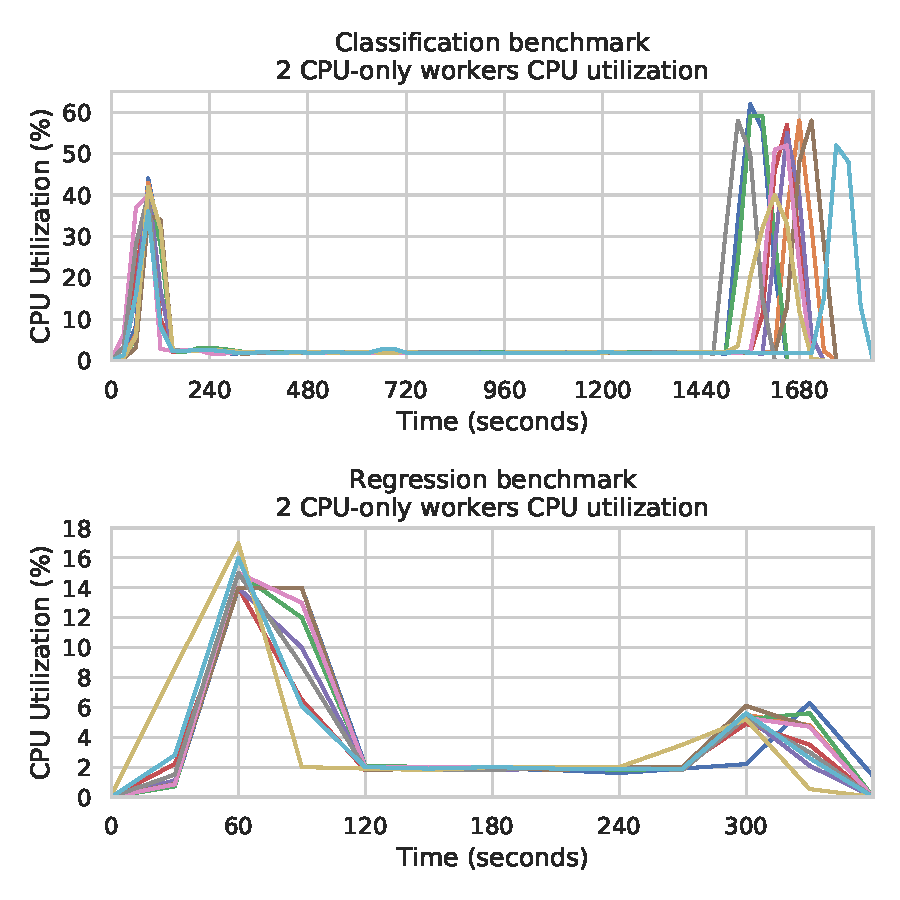
\includegraphics[scale=0.9]{images/07_evaluation/overall_auto-scaler_iterations}
\caption{CPU utilization during all iterations of both benchmarks with 2 CPU-only workers}
\label{fig:07_auto-scaler_iterations_results}
\end{figure}
% Max worker
To prevent an cluster over-provisioning, the maximum number of worker nodes for the classification benchmark is set to 15, and 10 for the regression benchmark.
% recurrence
\Fig{fig:07_auto-scaler_iterations_results} shows all 10 iterations of the CPU-only experiment for both benchmarks. It shows that, while the machine learning model is trained, only 2 performance spikes occurred at the beginning and at the end during a short time period. To scale while these performance spikes occur, the recurrence factor is set to 1. Additionally, the maximum CPU utilization for both benchmarks is set in accordance to the maximum CPU utilization during the performance spikes.
% The configurations
\begin{table}[ht]
\centering
\begin{tabular}{@{}l|ll@{}}
\toprule
Parameter               & Classification & Regression \\ \midrule
Interval                & 5 seconds      & 5 seconds  \\
Recurrence factor       & 1              & 1          \\
Cooldown period         & 60 seconds     & 60 seconds \\
Target CPU utilization  & 10\%           & 5\%        \\
Minimum CPU utilization & 5\%           & 2\%       \\
Maximum CPU utilization & 25\%           & 10\%       \\
Minimum worker nodes    & 2              & 2         \\
Maximum worker nodes    & 15              & 10         \\ \bottomrule
\end{tabular}
\caption{\textit{Auto-Scaler} configuration parameters for both benchmarks}
\label{table:07_auto-scaler_config_parameter}
\end{table}


\subsection{Execution Time Evaluation}
% Figure
\begin{figure}[h]
\centering
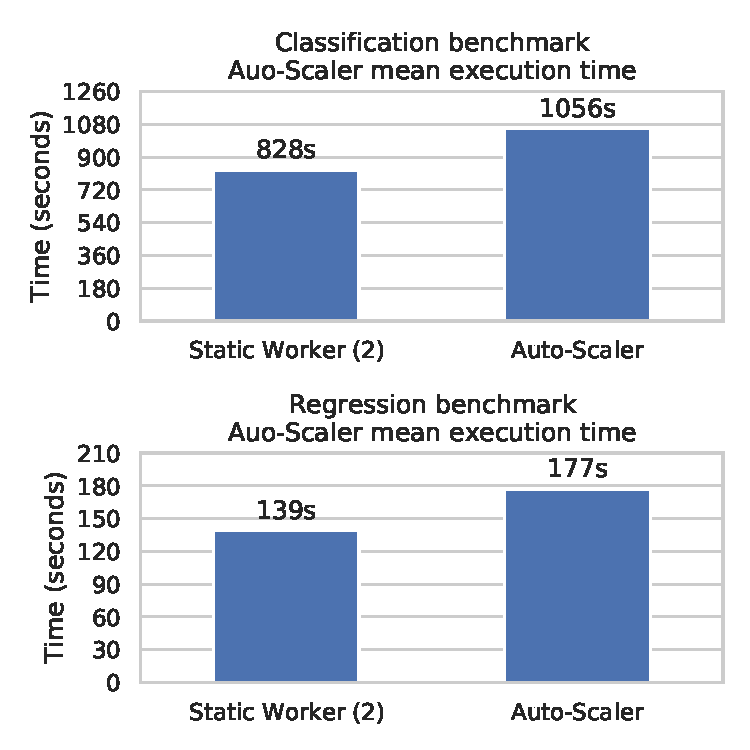
\includegraphics[scale=0.9]{images/07_evaluation/overall_auto-scaler}
\caption{\textit{Auto-Scaler} experiment mean execution time of both benchmarks}
\label{fig:07_auto-scaler_results}
\end{figure}

\paragraph{}
% Figure
\Fig{fig:07_auto-scaler_results} illustrates the results of the \textit{Auto-Scaler} experiment. The mean execution time of 2 CPU-only worker nodes is plotted against the mean execution time of the \textit{Auto-Scaler} experiment.
% Explain
The results show, that no improvement was achieved using the \textit{Auto-Scaler} implementation.
% Results
For the classification benchmark, the execution time of 2 CPU-only worker nodes increased by 228 seconds when enabling the \textit{Auto-Scaler} in the environment. Furthermore, the regression benchmark execution for 2 CPU-only worker nodes increased by 38 seconds with the the \textit{Auto-Scaler} enabled.

\paragraph{}
% Table
\begin{table}[ht]
\centering
\begin{tabular}{@{}l|ll|ll@{}}
\toprule
                               & \multicolumn{2}{c|}{Classification}                   & \multicolumn{2}{c}{Regression}                       \\
\multicolumn{1}{c|}{Iteration} & \multicolumn{1}{c}{Time} & \multicolumn{1}{c|}{Nodes} & \multicolumn{1}{c}{Time} & \multicolumn{1}{c}{Nodes} \\ \midrule
1  & \textbf{840s} & 15 & 168s          & 5 \\
2  & 960s          & 7  & \textbf{150s} & 2 \\
3  & 1020s         & 15 & 186s          & 6 \\
4  & 1140s         & 15 & 180s          & 6 \\
5  & 1080s         & 15 & 180s          & 6 \\
6  & 1140s         & 15 & 180s          & 6 \\
7  & 1140s         & 15 & 180s          & 6 \\
8  & 1080s         & 15 & 180s          & 6 \\
9  & 1140s         & 7  & 180s          & 6 \\
10 & 1020s         & 15 & 186s          & 6 \\ \bottomrule
\end{tabular}
\caption{Results of each iteration during the \textit{Auto-Scaler} experiment for both benchmarks}
\label{table:07_auto-scaler_iterations}
\end{table}
% Explain
\Tab{table:07_auto-scaler_iterations} summarizes the results for all 10 iterations of each benchmark.
% classification
For the classification benchmark, the best result was achieved in the first iteration with an execution time of 960 seconds and a maximum number of 15 worker nodes during the execution.
% regression
The regression benchmark achieved best in the second iteration, with an execution time of 150 seconds and a maximum number of 2 worker nodes during this iteration.
% n maximum reached
The results show that during the classification benchmark experiment, the \textit{Auto-Scaler} added the maximum number of allowed worker nodes in 8 out of 10 iterations. During the regression benchmark experiment, the maximum number of worker nodes was never reached. Furthermore, in the second iteration, when the best result was achieved, the \textit{Auto-Scaler} has not scaled the number of worker nodes.

\paragraph{}
% Meaning
The performance decrease when enabling the Auto-Scaler is possibly caused by the lack of efficient workload distribution by Apache Spark.


\section{Experimental Results Summary}
% Intro
The experimental results show, that GPU-accelerated worker nodes significantly outperform worker nodes using only CPUs.
% Auto-scaler
However, the \textit{Auto-Scaler} was not able to improve the performance of the computing environment.
%
Moreover, enabling the \textit{Auto-Scaler} during the training of machine learning models increased the execution time of active performing spark-jobs.

\chapter{Outlook}
\label{chap:08_outlook}

In this chapter , an outlook is given for further research based on the results of \Chap{chap:07_evaluation}.


% ===========================================
% ===========================================
\section{Scaling}
% Intro
The results of SECTION XY show that, the implementation of the Auto-Scaler is nit sufficient for scaling Apache Spark worker nodes. Furthermore, it has increased the overall execution time for a spark-job.


% Reasons
A possible reason for this is result is, that Apache Spark is not able to efficiently distribute the workload between existing worker nodes and newly created worker nodes.
% a solution
A solution for this problem is, to activate worker nodes when they are needed instead of deploying new nodes. Apache Spark supports to blacklist worker nodes to creates executors.
% the concept
Then, instead of deploying new worker nodes, the Auto-Scaler whitelists a specific number of already existing worker.


% Reactive scaler
The current design of the Auto-Scaler follows a proactive approach by responding to the current status of the computing environment (see SEC RELATED WORK).
% pro active
The efficiency of the Auto-Scaler can be optimized by following a reactive approach. Then the Auto-Scaler uses techniques to predict the future state of the computing environment.
% MAPE-K
The MAPE architecture used for the autonomic manager can be extended to gain knowledge (MAPE-K).
% reinformcement learning
The knowledge can be used to predict the future state of the computing environment using reinforcement-learning models.


% scaling executor
In the experiment of CHAP EVAL, all workers only executed their work on one executor.
% another approach
The number of executors can be scaled as well.
% Rapids
In accordance with the RAPIDS plugin, for each executor 1 GPU has to be available.



% Vertical scaling
Another approach to scale the performance of Apache Spark worker is vertical scaling.
% in this thesis
In this thesis, the horizontal scaling approach is used to scale the number of actively performing worker nodes.
%
By using the vertical scaling approach, the resources of executors can be scaled. This can have the effect, that a worker is able to compute faster.


% ===========================================
% ===========================================
\section{Shuffle bla bla}
As mentioned in SECTION DESIGN ODER IMPL, the current approach is, that no worker nodes are removed while applications re actively performed.
% Why
Worker nodes cant be removed while applications are performed because each participating worker, keeps temporary data. If a node is removed, the application will not succeed.
%
To remove worker while applications are perform to prevent over-provisioning, an external shuffle service is needed. This enabled worker to store temporary data on an external node which is available across all worker nodes.
% blacklisting
Additional it is necessary to blacklist nodes which will be removed, so no executor will be deployed on that node.
%
Zeus, apaches external shuffle service.

\chapter{Conclusion}
\label{sec:conclusion}
%
\todo{Describe Chapter}

\section{Cluster architecture}


%\fi

% Anhang (Bibliographie darf im deutschen nicht in den Anhang!)
\bibliography{literatur}
%\nocite{*}
\clearpage

% Anhang
\appendix
% 'Anhang' ins Inhaltsverzeichnis
\phantomsection
\addcontentsline{toc}{part}{Anhang}
\chapter{Computing Environment Implementation}

\begin{lstlisting}[label=lst:appendix_env_compose, caption=Computing environment docker-compose file]
version: "3.7"
 
networks:
    computing-net:
        name: computing_net
        attachable: true
 
services:
    spark-master:
        image: spark-master:3.0.1-hadoop2.7
        networks:
            - computing-net
        ports:
            - 4040:4040
            - 7077:7077
        volumes:
            - ./conf/spark-master/metrics.properties:/usr/bin/spark/conf/metrics.properties
            - ./conf/spark-master/spark-defaults.conf:/usr/bin/spark/conf/spark-defaults.conf
 
    prometheus:
        image: prom/prometheus
        networks:
            - computing-net
        volumes:
            - ./conf/prometheus/prometheus.yml:/etc/prometheus/prometheus.yml
            - ./conf/prometheus/recording_rules.yml:/etc/prometheus/recording_rules.yml
        command:
            - "--config.file=/etc/prometheus/prometheus.yml"
        ports:
            - "9090:9090"
        depends_on:
            - cadvisor
 
    cadvisor:
        image: google/cadvisor
        networks:
            - computing-net
        ports:
            - "8080:8080"
        volumes:
            - "/:/rootfs:ro"
            - "/var/run:/var/run:ro"
            - "/sys:/sys:ro"
            - "/var/lib/docker/:/var/lib/docker:ro"
            - "/dev/disk/:/dev/disk:ro"
        command:
            - "--docker_only=true"
            - "--logtostderr=true"
        depends_on:
            - spark-master
            - spark-worker
 
    auto-scaler:
        image: auto-scaler:latest
        networks:
            - computing-net
        volumes:
            - "/var/run/docker.sock:/var/run/docker.sock:ro"
            - ./conf/auto-scaler/config.yml:/etc/autoscaler/config.yml
        command:
            - '--config=/etc/autoscaler/config.yml'
        depends_on:
            - prometheus
\end{lstlisting}

\chapter{Apache Spark Cluster Implementation}

% Base image dockerfile
\begin{lstlisting}[label=lst:appendix_spark_base_dockerfile, caption=Apache Spark base image Dockerfile]
FROM nvidia/cuda:11.0-devel-ubuntu16.04
 
LABEL maintainer="marcel.pascal.stolin@ipa.fraunhofer.de"
 
ARG SPARK_VERSION
ARG HADOOP_VERSION
 
# Install all important packages
RUN apt-get update -qy && \
    apt-get install -y openjdk-8-jre-headless procps python3 python3-pip curl
 
# Install Apache Spark
RUN mkdir /usr/bin/spark/ && \
    curl https://ftp-stud.hs-esslingen.de/pub/Mirrors/ftp.apache.org/dist/spark/spark-${SPARK_VERSION}/spark-${SPARK_VERSION}-bin-hadoop${HADOOP_VERSION}.tgz -o spark.tgz && \
    tar -xf spark.tgz && \
    mv spark-${SPARK_VERSION}-bin-hadoop${HADOOP_VERSION}/* /usr/bin/spark/ && \
    rm -rf spark.tgz && \
    rm -rf spark-${SPARK_VERSION}-bin-hadoop${HADOOP_VERSION}/
 
# Add GPU discovery script
RUN mkdir /opt/sparkRapidsPlugin/
COPY getGpusResources.sh /opt/sparkRapidsPlugin/getGpusResources.sh
ENV SPARK_RAPIDS_DIR=/opt/sparkRapidsPlugin
 
# Install cuDF and RAPIDS
RUN curl -o ${SPARK_RAPIDS_DIR}/cudf-0.15-cuda11.jar https://repo1.maven.org/maven2/ai/rapids/cudf/0.15/cudf-0.15-cuda11.jar
RUN curl -o ${SPARK_RAPIDS_DIR}/rapids-4-spark_2.12-0.2.0.jar https://repo1.maven.org/maven2/com/nvidia/rapids-4-spark_2.12/0.2.0/rapids-4-spark_2.12-0.2.0.jar
ENV SPARK_CUDF_JAR=${SPARK_RAPIDS_DIR}/cudf-0.15-cuda11.jar
ENV SPARK_RAPIDS_PLUGIN_JAR=${SPARK_RAPIDS_DIR}/rapids-4-spark_2.12-0.2.0.jar
 
# Set all environment variables
ENV JAVA_HOME=/usr/lib/jvm/java-8-openjdk-amd64
ENV SPARK_HOME /usr/bin/spark
ENV SPARK_NO_DAEMONIZE true
ENV PYSPARK_DRIVER_PYTHON python3
ENV PYSPARK_PYTHON python3
ENV PATH /usr/bin/spark/bin:/usr/bin/spark/sbin:$PATH
 
WORKDIR ${SPARK_HOME}
\end{lstlisting}


% Master image dockerfile
\begin{lstlisting}[label=lst:appendix_spark_master_dockerfile, caption=Apache Spark master image Dockerfile]
ARG SPARK_VERSION
ARG HADOOP_VERSION
 
FROM spark-base:$SPARK_VERSION-hadoop$HADOOP_VERSION
 
LABEL maintainer="marcel.pascal.stolin@ipa.fraunhofer.de"
 
# Set ports
ENV SPARK_MASTER_PORT 7077
ENV SPARK_MASTER_WEBUI_PORT 4040
 
EXPOSE 4040 7077
 
# Start master-node in standalone mode
ENTRYPOINT [ "sbin/start-master.sh" ]
\end{lstlisting}


% Worker image Dockerfile
\begin{lstlisting}[label=lst:appendix_spark_worker_dockerfile, caption=Apache Spark worker image Dockerfile]
ARG SPARK_VERSION
ARG HADOOP_VERSION
 
FROM spark-base:$SPARK_VERSION-hadoop$HADOOP_VERSION
 
LABEL maintainer="marcel.pascal.stolin@ipa.fraunhofer.de"
 
# Add spark-env
COPY spark-env.sh ${SPARK_HOME}/conf/spark-env.sh
 
# Set port
ENV SPARK_WORKER_WEBUI_PORT 4041
 
EXPOSE 4041
 
# Start worker-node
ENTRYPOINT ./sbin/start-slave.sh ${SPARK_MASTER_URI}
\end{lstlisting}


% GPU discovery script
\begin{lstlisting}[label=lst:appendix_spark_gpu-discovery, caption=GPU discovery script - Source: \url{https://github.com/apache/spark/blob/v3.0.1/examples/src/main/scripts/getGpusResources.sh} (Accessed: 2021-01-03), language=bash]
#!/usr/bin/env bash

#
# Licensed to the Apache Software Foundation (ASF) under one or more
# contributor license agreements.  See the NOTICE file distributed with
# this work for additional information regarding copyright ownership.
# The ASF licenses this file to You under the Apache License, Version 2.0
# (the "License"); you may not use this file except in compliance with
# the License.  You may obtain a copy of the License at
#
#    http://www.apache.org/licenses/LICENSE-2.0
#
# Unless required by applicable law or agreed to in writing, software
# distributed under the License is distributed on an "AS IS" BASIS,
# WITHOUT WARRANTIES OR CONDITIONS OF ANY KIND, either express or implied.
# See the License for the specific language governing permissions and
# limitations under the License.
#

# This script is a basic example script to get resource information about NVIDIA GPUs.
# It assumes the drivers are properly installed and the nvidia-smi command is available.
# It is not guaranteed to work on all setups so please test and customize as needed
# for your environment. It can be passed into SPARK via the config
# spark.{driver/executor}.resource.gpu.discoveryScript to allow the driver or executor to discover
# the GPUs it was allocated. It assumes you are running within an isolated container where the
# GPUs are allocated exclusively to that driver or executor.
# It outputs a JSON formatted string that is expected by the
# spark.{driver/executor}.resource.gpu.discoveryScript config.
#
# Example output: {"name": "gpu", "addresses":["0","1","2","3","4","5","6","7"]}

ADDRS=`nvidia-smi --query-gpu=index --format=csv,noheader | sed -e ':a' -e 'N' -e'$!ba' -e 's/\n/","/g'`
echo {\"name\": \"gpu\", \"addresses\":[\"$ADDRS\"]}
\end{lstlisting}

% Custom submit script
\begin{lstlisting}[label=lst:appendix_spark-submit_script, caption=Custom submit script, language=sh]
#!/bin/bash
 
DRIVER_MEMORY=${DRIVER_MEMORY-4g}
EXECUTOR_MEMORY=${EXECUTOR_MEMORY-8g}
 
if [ "$CPU_ONLY" == "true" ]
    then
    echo "Submit Spark app with CPU only"
 
    $SPARK_HOME/bin/spark-submit \
        --master $SPARK_MASTER_URI \
        --driver-memory $DRIVER_MEMORY \
        --executor-memory $EXECUTOR_MEMORY \
        --conf spark.driver.extraClassPath=${SPARK_CUDF_JAR}:${JAR_RAPIDS}:${LIBS_PATH}/xgboost4j_3.0-1.3.0-0.1.0.jar:${LIBS_PATH}/xgboost4j-spark_3.0-1.3.0-0.1.0.jar \
        --conf spark.executor.extraClassPath=${SPARK_CUDF_JAR}:${JAR_RAPIDS}:${LIBS_PATH}/xgboost4j_3.0-1.3.0-0.1.0.jar:${LIBS_PATH}/xgboost4j-spark_3.0-1.3.0-0.1.0.jar \
        --jars ${SPARK_CUDF_JAR},${LIBS_PATH}/xgboost4j-spark_3.0-1.3.0-0.1.0.jar,${LIBS_PATH}/xgboost4j_3.0-1.3.0-0.1.0.jar,${JAR_RAPIDS} \
        --py-files ${LIBS_PATH}/xgboost4j-spark_3.0-1.3.0-0.1.0.jar,/tank/data/users/chh-ms/spark-xgboost-examples/examples/apps/python/samples.zip \
        $@
else
    echo "Submit Spark app with GPU acceleration"
 
    RAPIDS_GPU_ALLOC_FRACTION=${RAPIDS_GPU_ALLOC_FRACTION-1}
    RAPIDS_INCOMPATIBLE_OPS=${RAPIDS_INCOMPATIBLE_OPS-"false"}
    RAPIDS_DEBUG=${RAPIDS_DEBUG-"NONE"}
    RAPIDS_GPU_POOL=${RAPIDS_GPU_POOL-"ARENA"}
 
    $SPARK_HOME/bin/spark-submit \
        --master $SPARK_MASTER_URI \
        --driver-memory $DRIVER_MEMORY \
        --executor-memory $EXECUTOR_MEMORY \
        --conf spark.plugins=com.nvidia.spark.SQLPlugin \
        --conf spark.rapids.memory.gpu.pool=$RAPIDS_GPU_POOL \
        --conf spark.rapids.memory.gpu.allocFraction=$RAPIDS_GPU_ALLOC_FRACTION \
        --conf spark.rapids.sql.incompatibleOps.enabled=$RAPIDS_INCOMPATIBLE_OPS \
        --conf spark.rapids.memory.gpu.debug=$RAPIDS_DEBUG \
        --conf spark.task.resource.gpu.amount=1 \
        --conf spark.executor.resource.gpu.amount=1 \
        --conf spark.driver.extraClassPath=${SPARK_CUDF_JAR}:${JAR_RAPIDS}:${LIBS_PATH}/xgboost4j_3.0-1.3.0-0.1.0.jar:${LIBS_PATH}/xgboost4j-spark_3.0-1.3.0-0.1.0.jar \
        --conf spark.executor.extraClassPath=${SPARK_CUDF_JAR}:${JAR_RAPIDS}:${LIBS_PATH}/xgboost4j_3.0-1.3.0-0.1.0.jar:${LIBS_PATH}/xgboost4j-spark_3.0-1.3.0-0.1.0.jar \
        --jars ${SPARK_CUDF_JAR},${LIBS_PATH}/xgboost4j-spark_3.0-1.3.0-0.1.0.jar,${LIBS_PATH}/xgboost4j_3.0-1.3.0-0.1.0.jar,${JAR_RAPIDS} \
        --py-files ${LIBS_PATH}/xgboost4j-spark_3.0-1.3.0-0.1.0.jar,/tank/data/users/chh-ms/spark-xgboost-examples/examples/apps/python/samples.zip \
        $@  
fi
\end{lstlisting}


\section{Evaluation Data}

\subsection{Classification Benchmarks}

\begin{figure}[h]
\centering
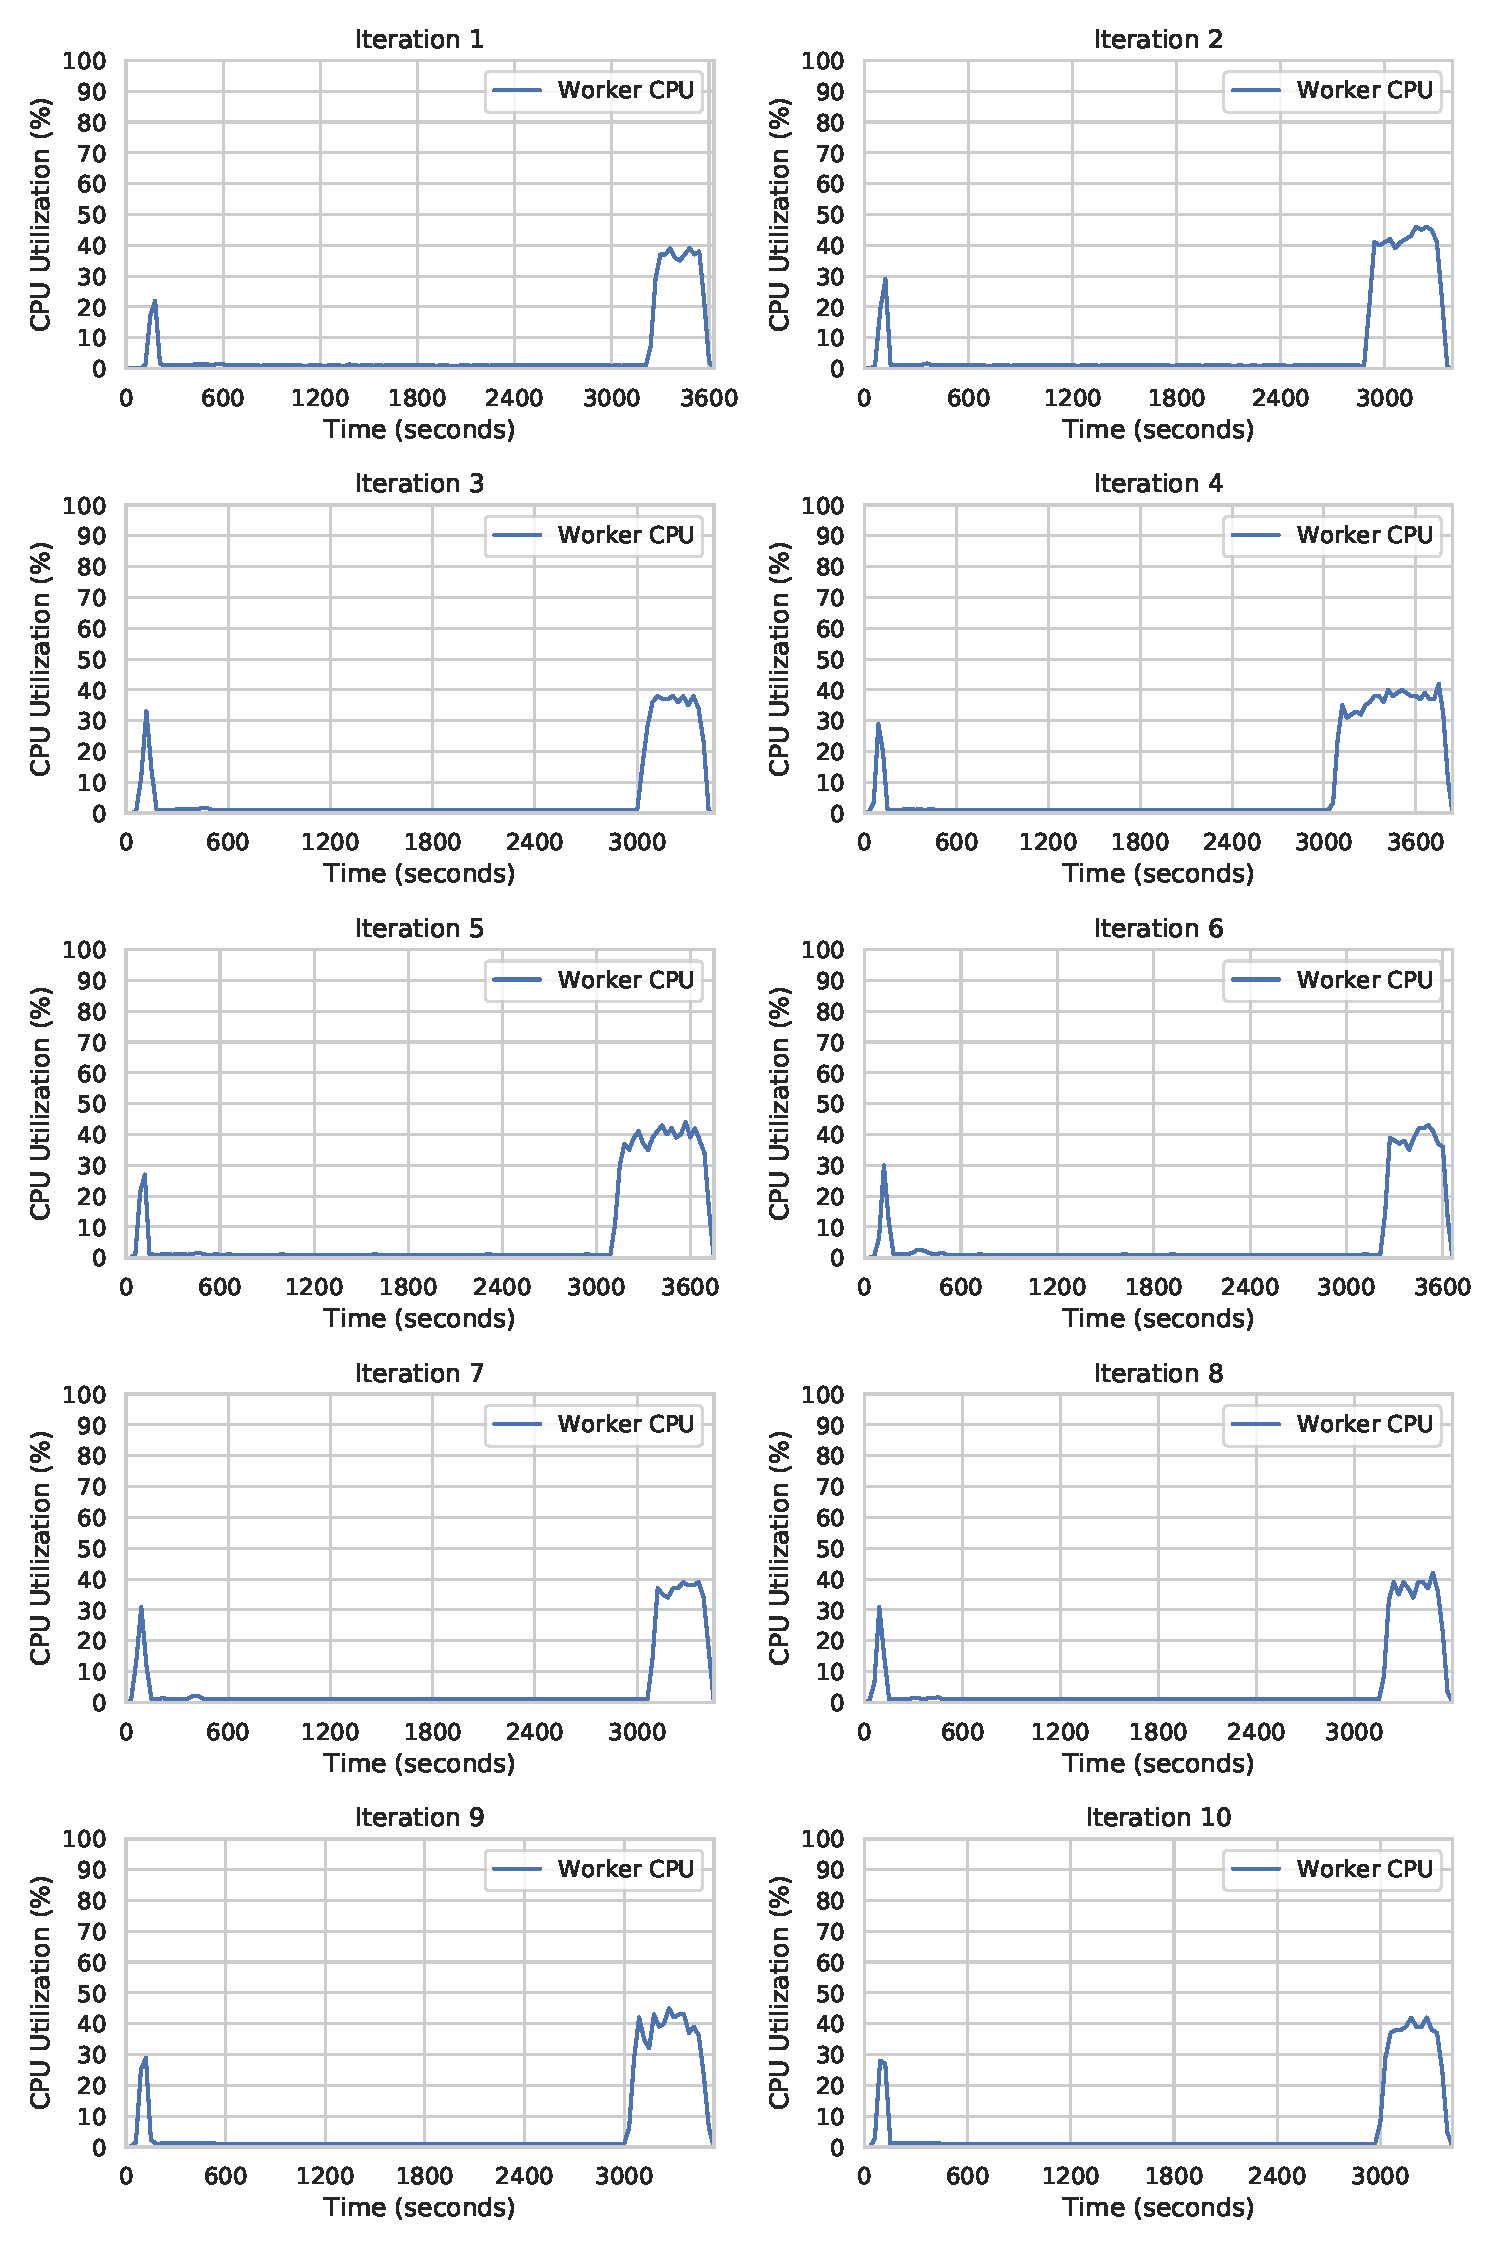
\includegraphics[scale=0.4]{images/07_evaluation/mortgage/mortgage_1_worker_cpu_performance}
\caption{Classification algorithm performance evaluation of the computing environment with 1 Apache Spark worker}
\label{fig:07_mortgage_static-cpu_results}
\end{figure}

\begin{figure}[h]
\centering
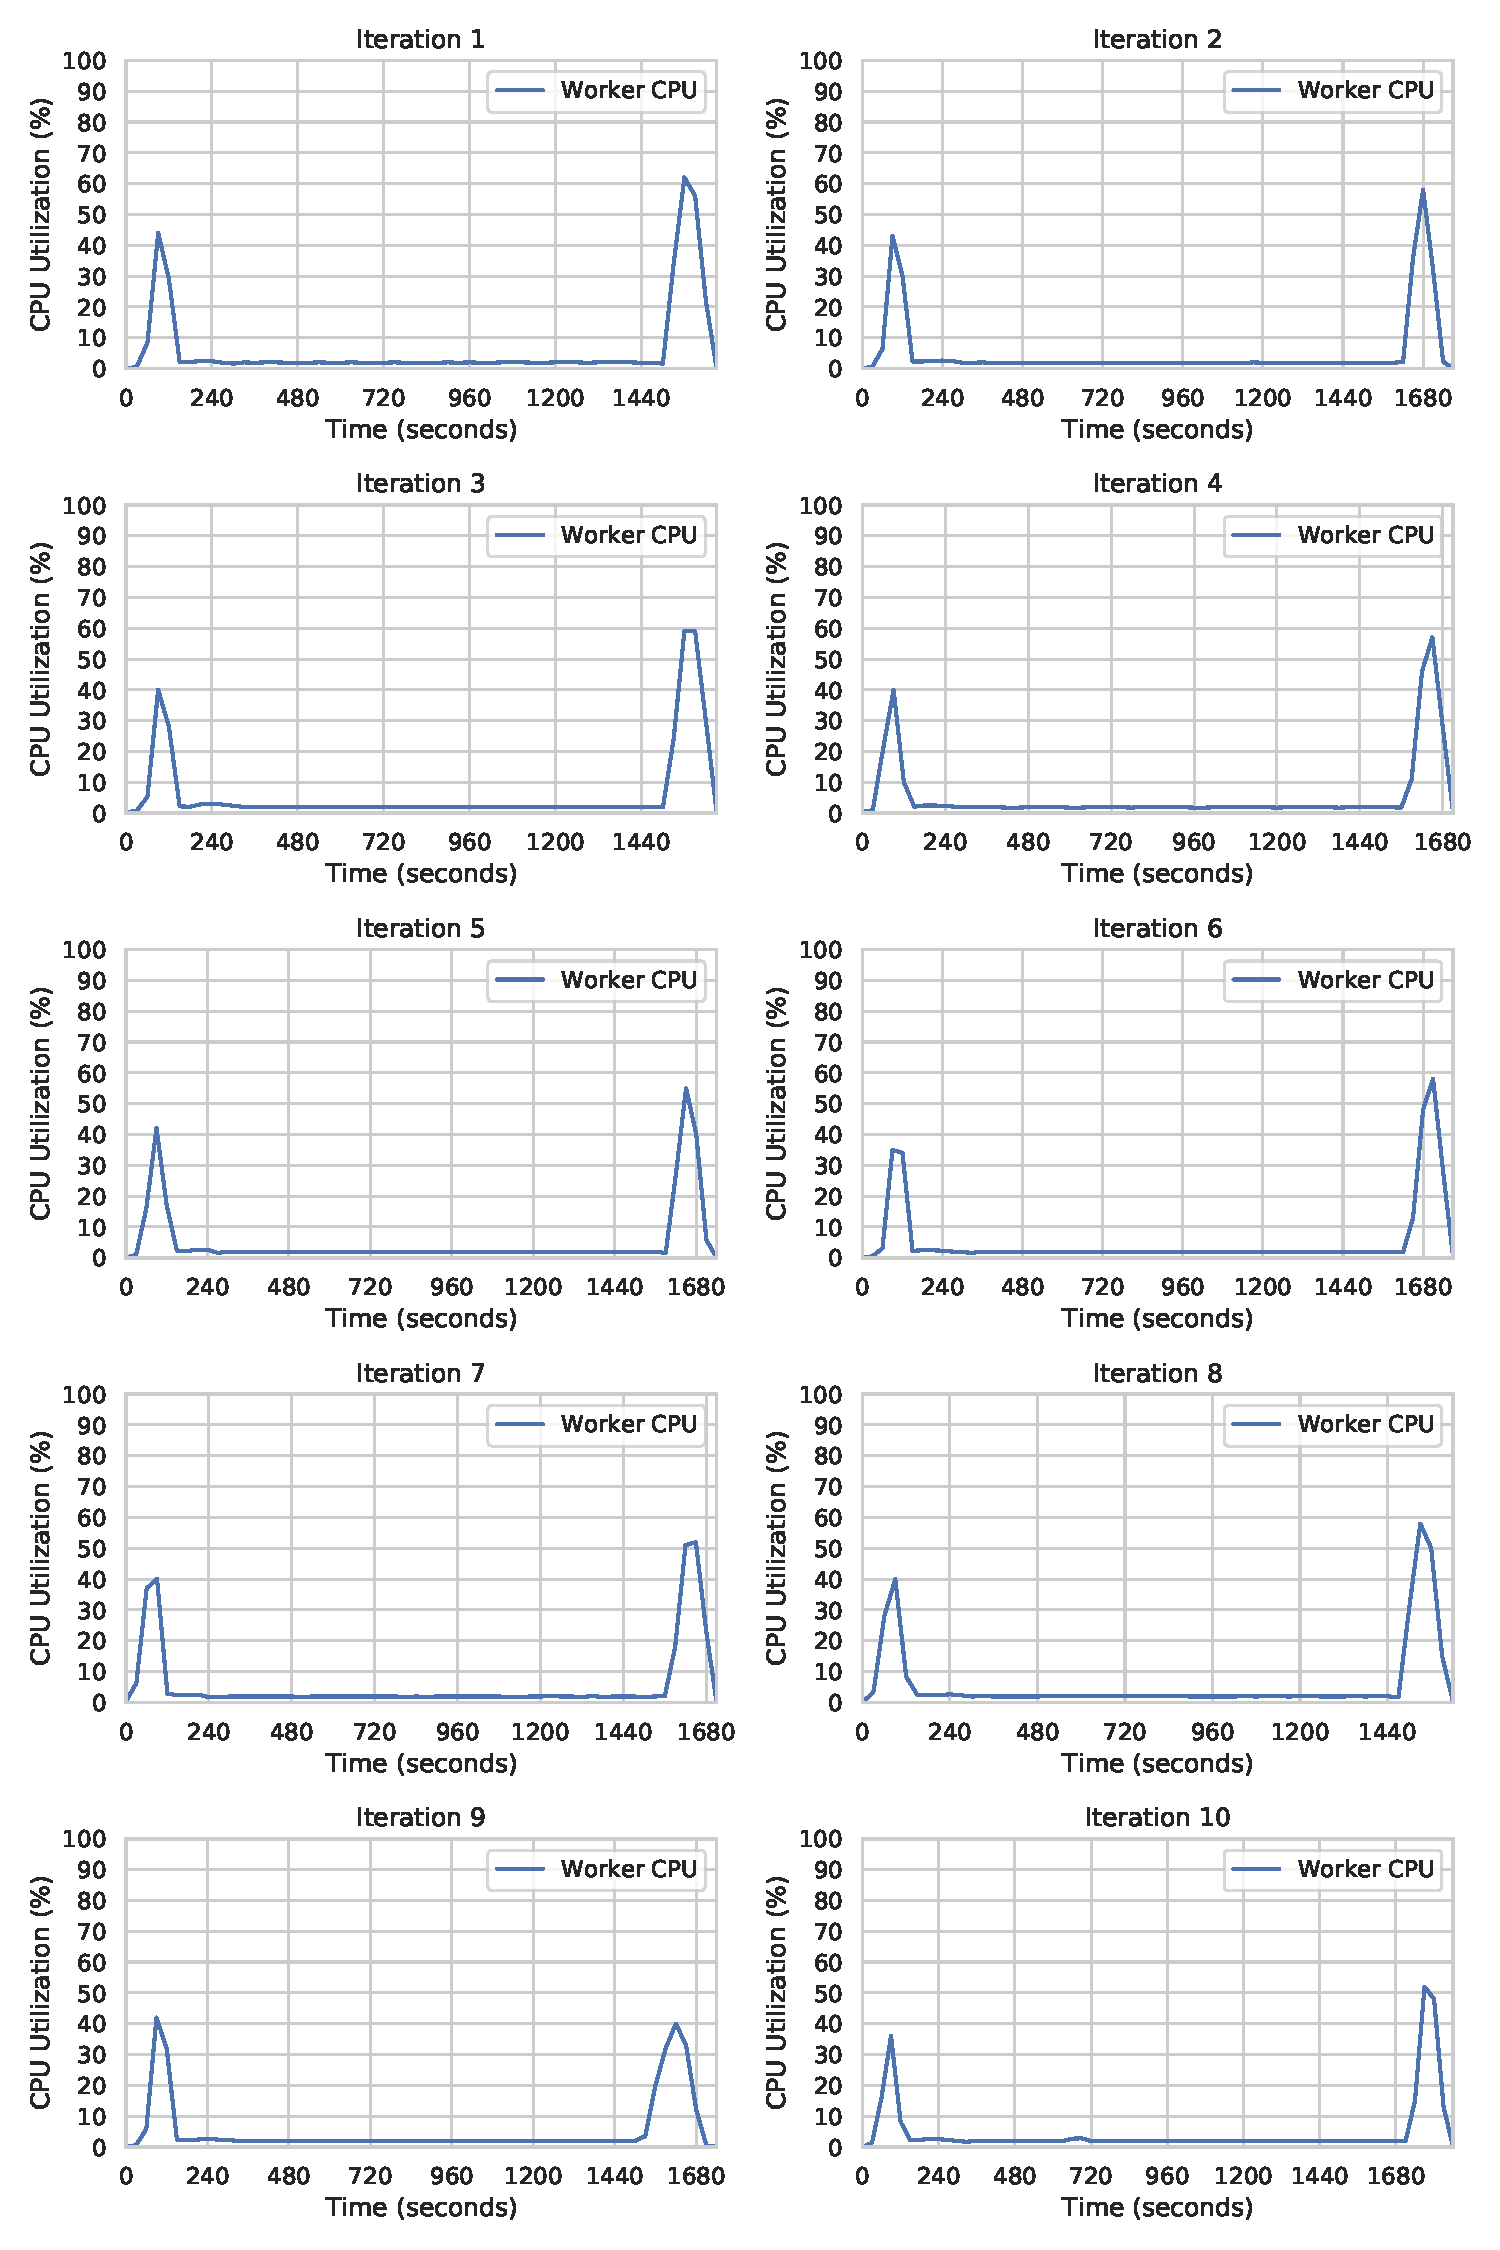
\includegraphics[scale=0.4]{images/07_evaluation/mortgage/mortgage_2_worker_cpu_performance}
\caption{Classification algorithm performance evaluation of the computing environment with 2 Apache Spark worker}
\label{fig:07_mortgage_static-cpu_results}
\end{figure}

\begin{figure}[h]
\centering
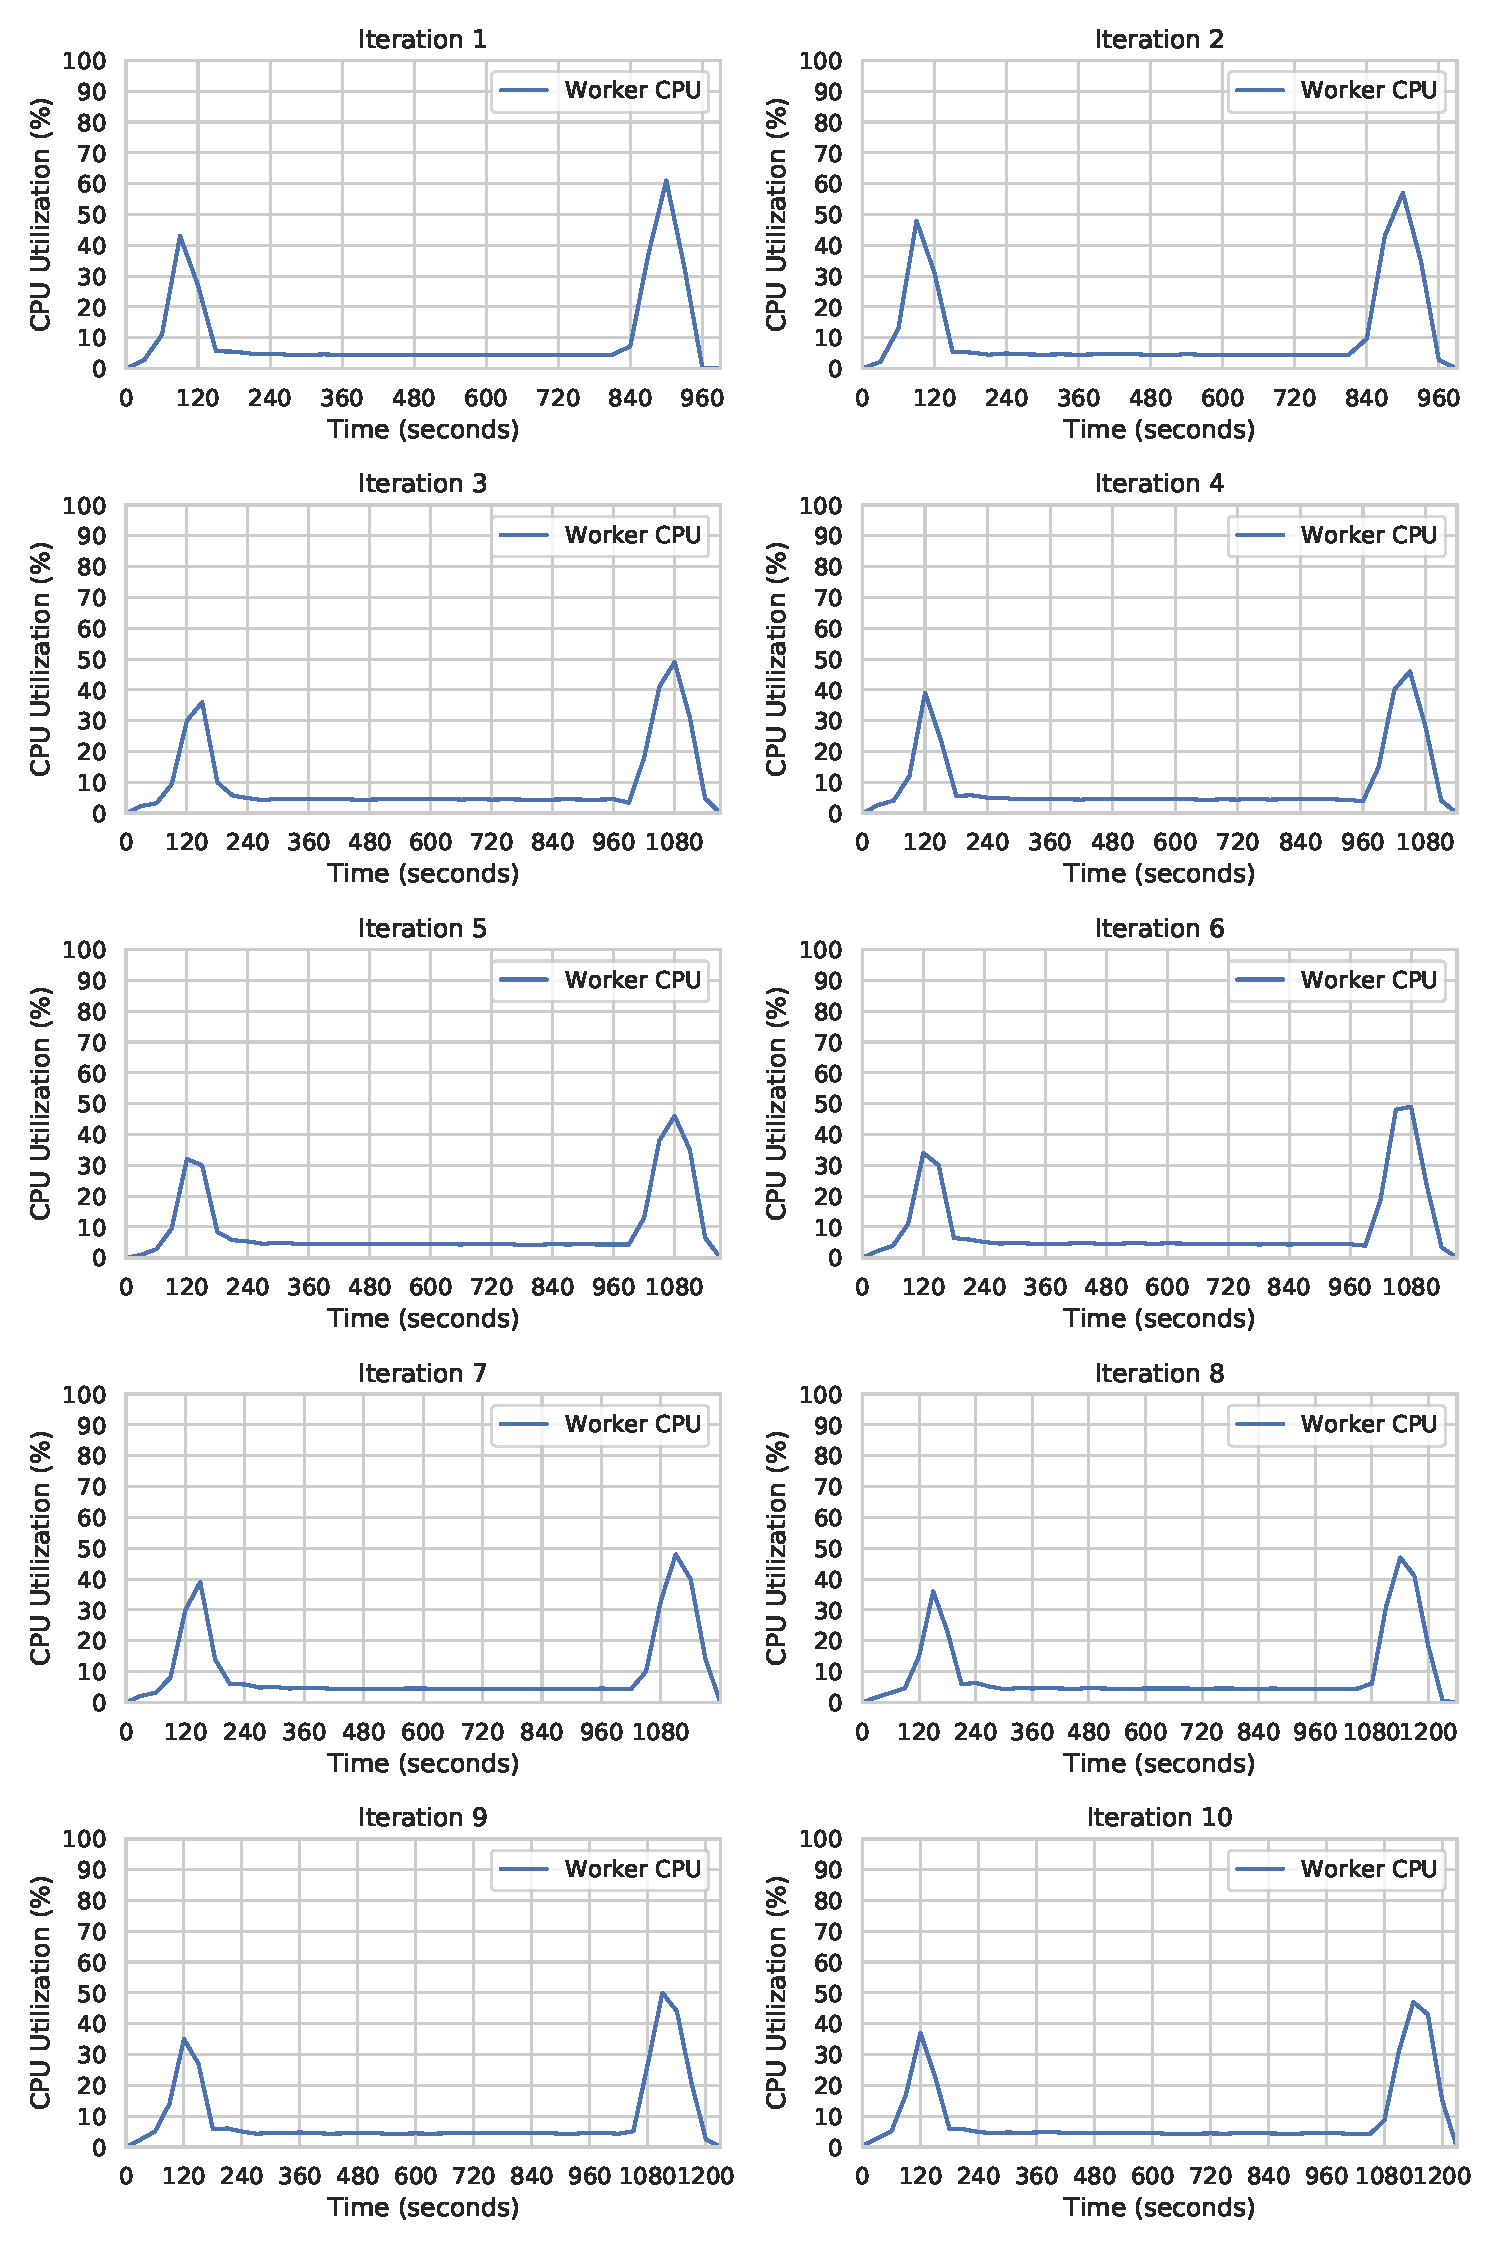
\includegraphics[scale=0.4]{images/07_evaluation/mortgage/mortgage_5_worker_cpu_performance}
\caption{Classification algorithm performance evaluation of the computing environment with 5 Apache Spark worker}
\label{fig:07_mortgage_static-cpu_results}
\end{figure}

\begin{figure}[h]
\centering
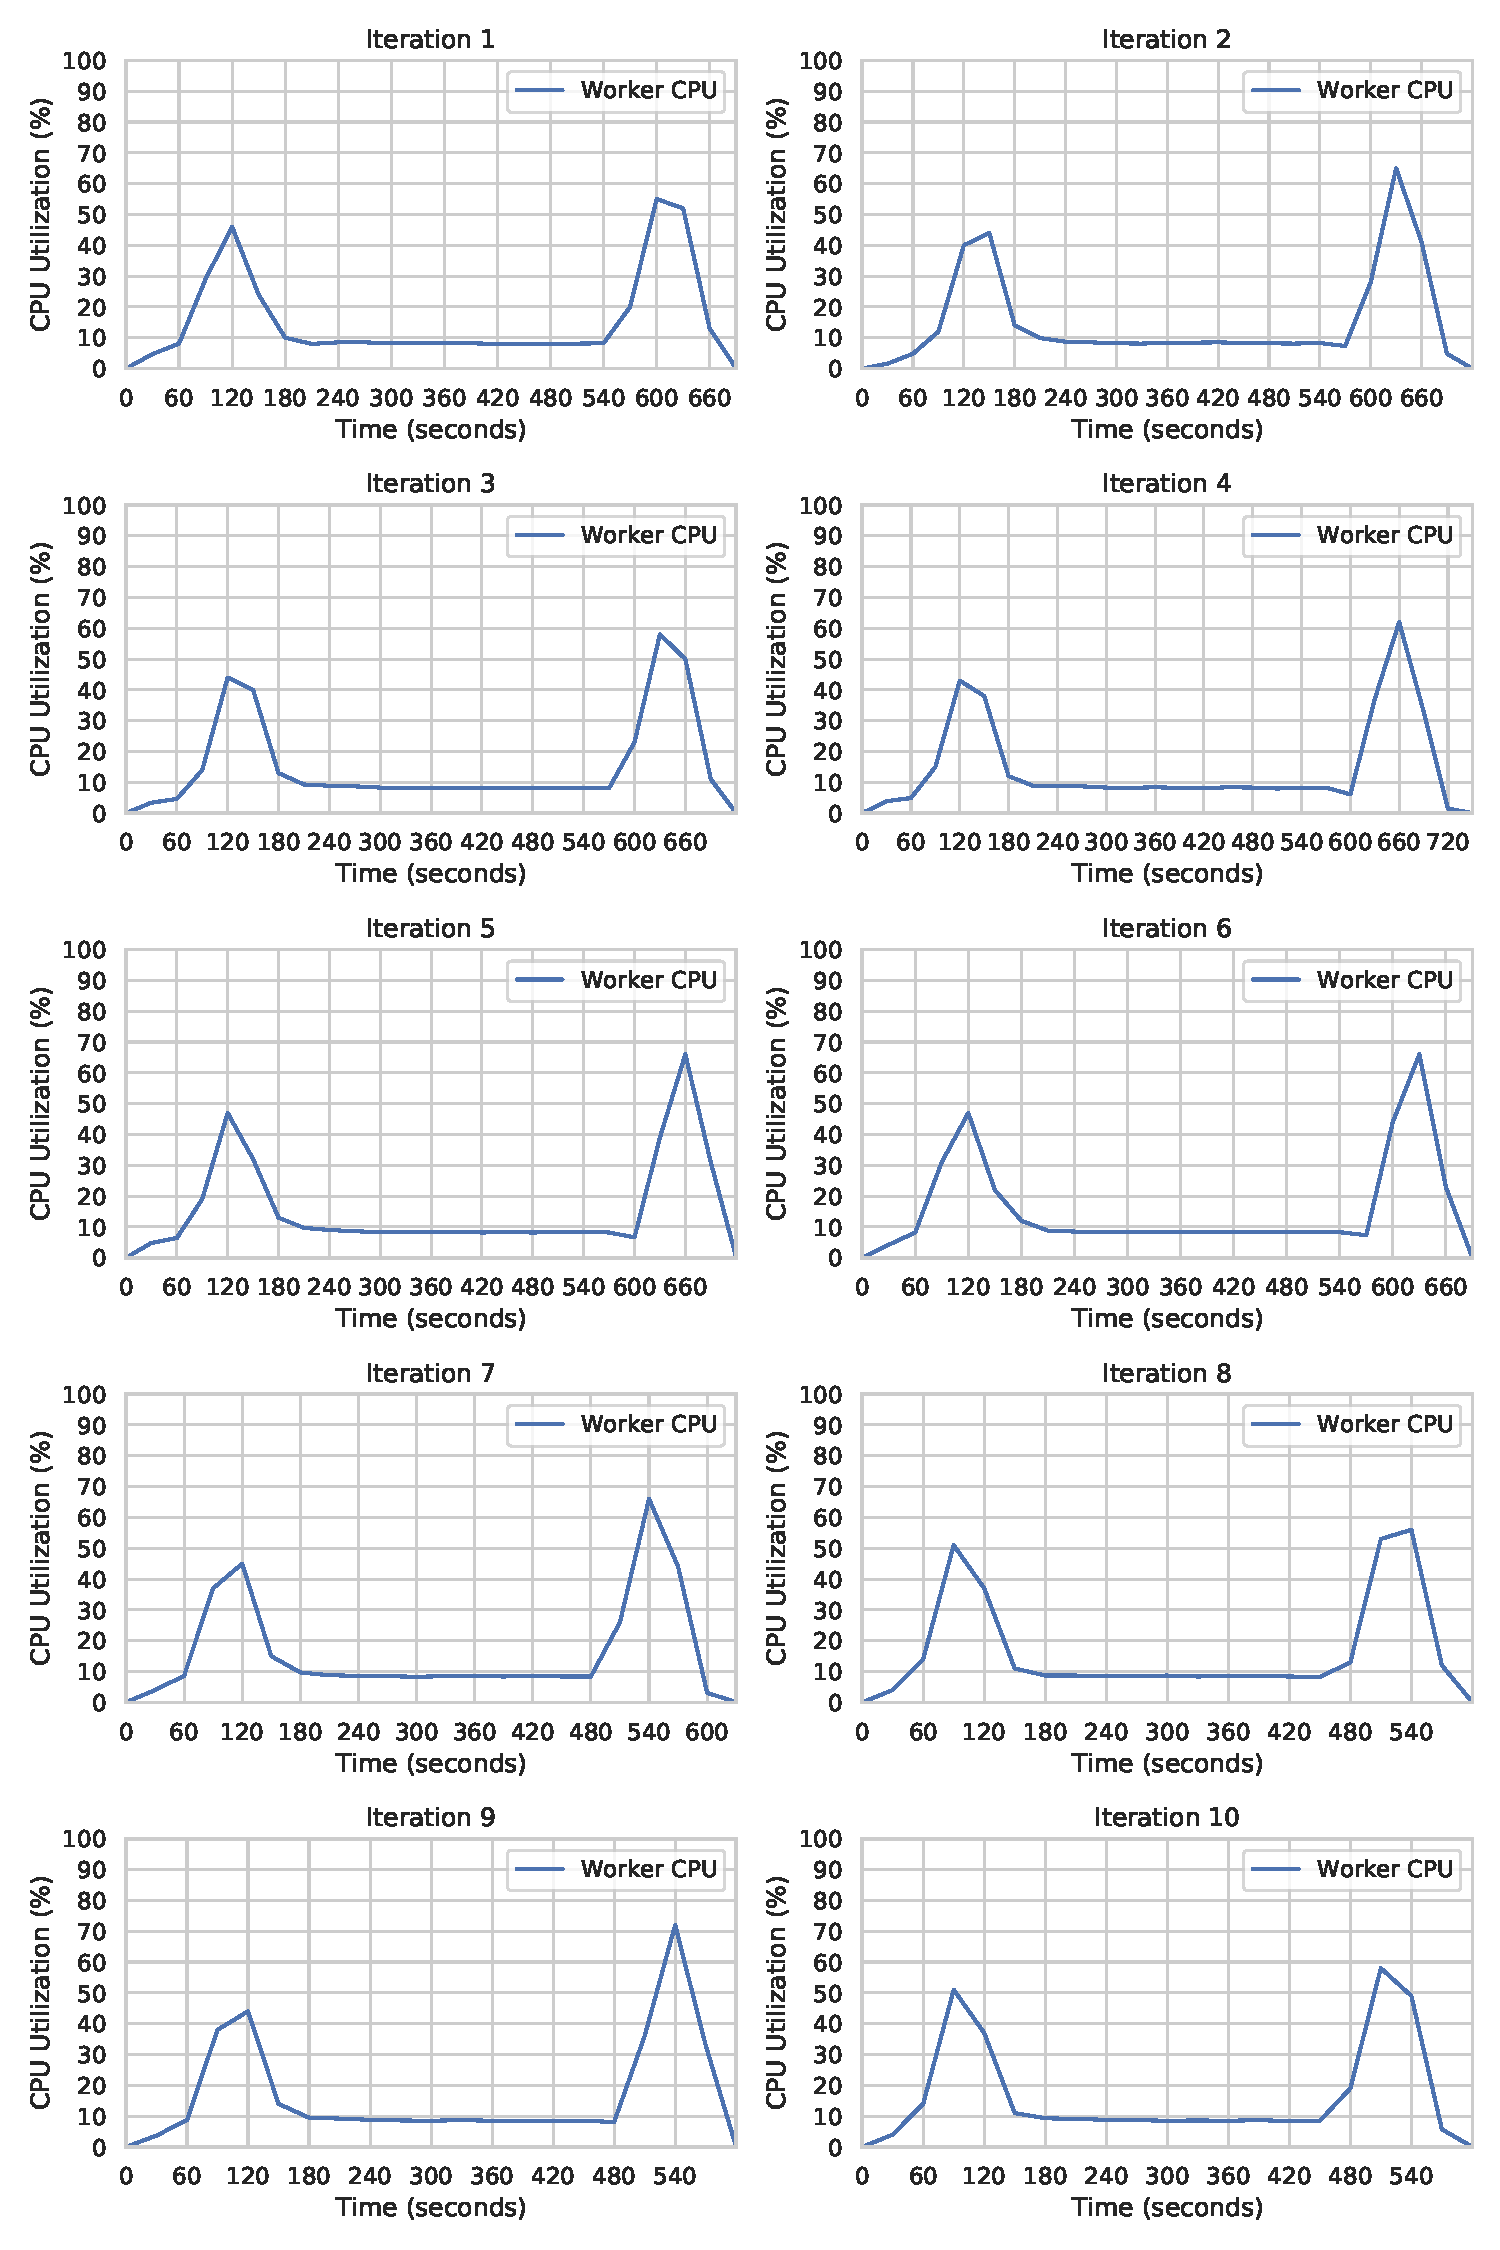
\includegraphics[scale=0.4]{images/07_evaluation/mortgage/mortgage_10_worker_cpu_performance}
\caption{Classification algorithm performance evaluation of the computing environment with 10 Apache Spark worker}
\label{fig:07_mortgage_static-cpu_results}
\end{figure}

\begin{figure}[h]
\centering
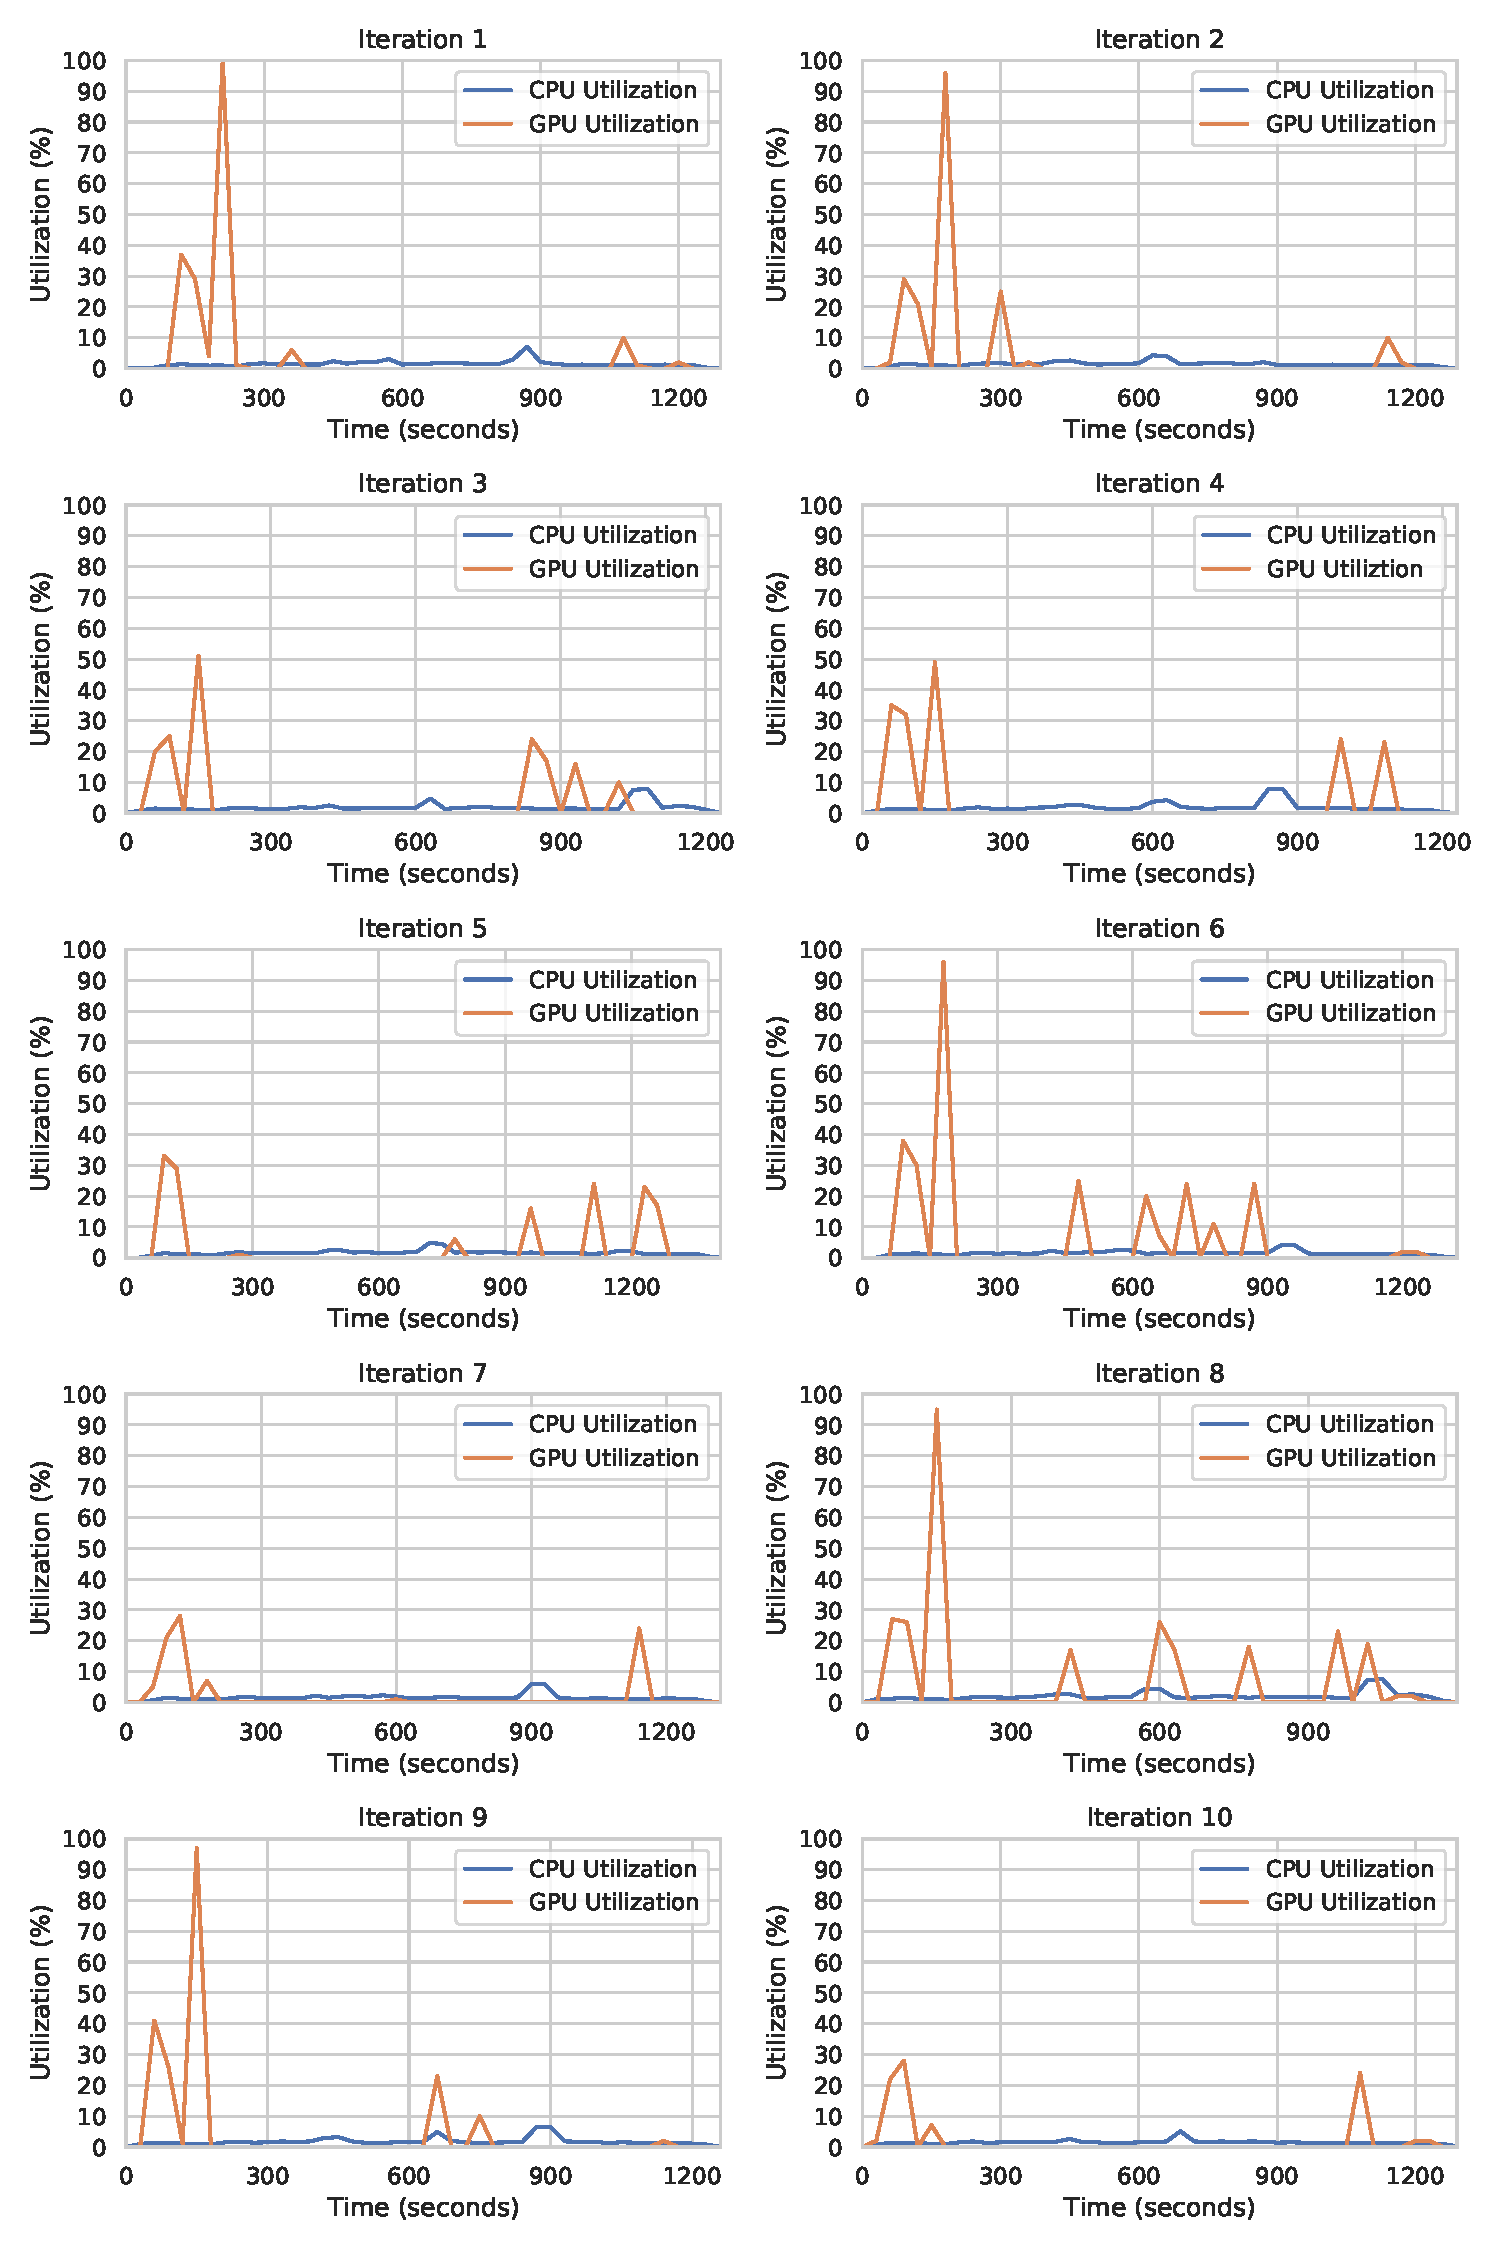
\includegraphics[scale=0.4]{images/07_evaluation/mortgage/mortgage_gpu1_performance}
\caption{Classification algorithm performance evaluation of the computing environment with 1 Apache Spark worker and GPU acceleration enabled}
\label{fig:07_mortgage_static-cpu_results}
\end{figure}

\begin{figure}[h]
\centering
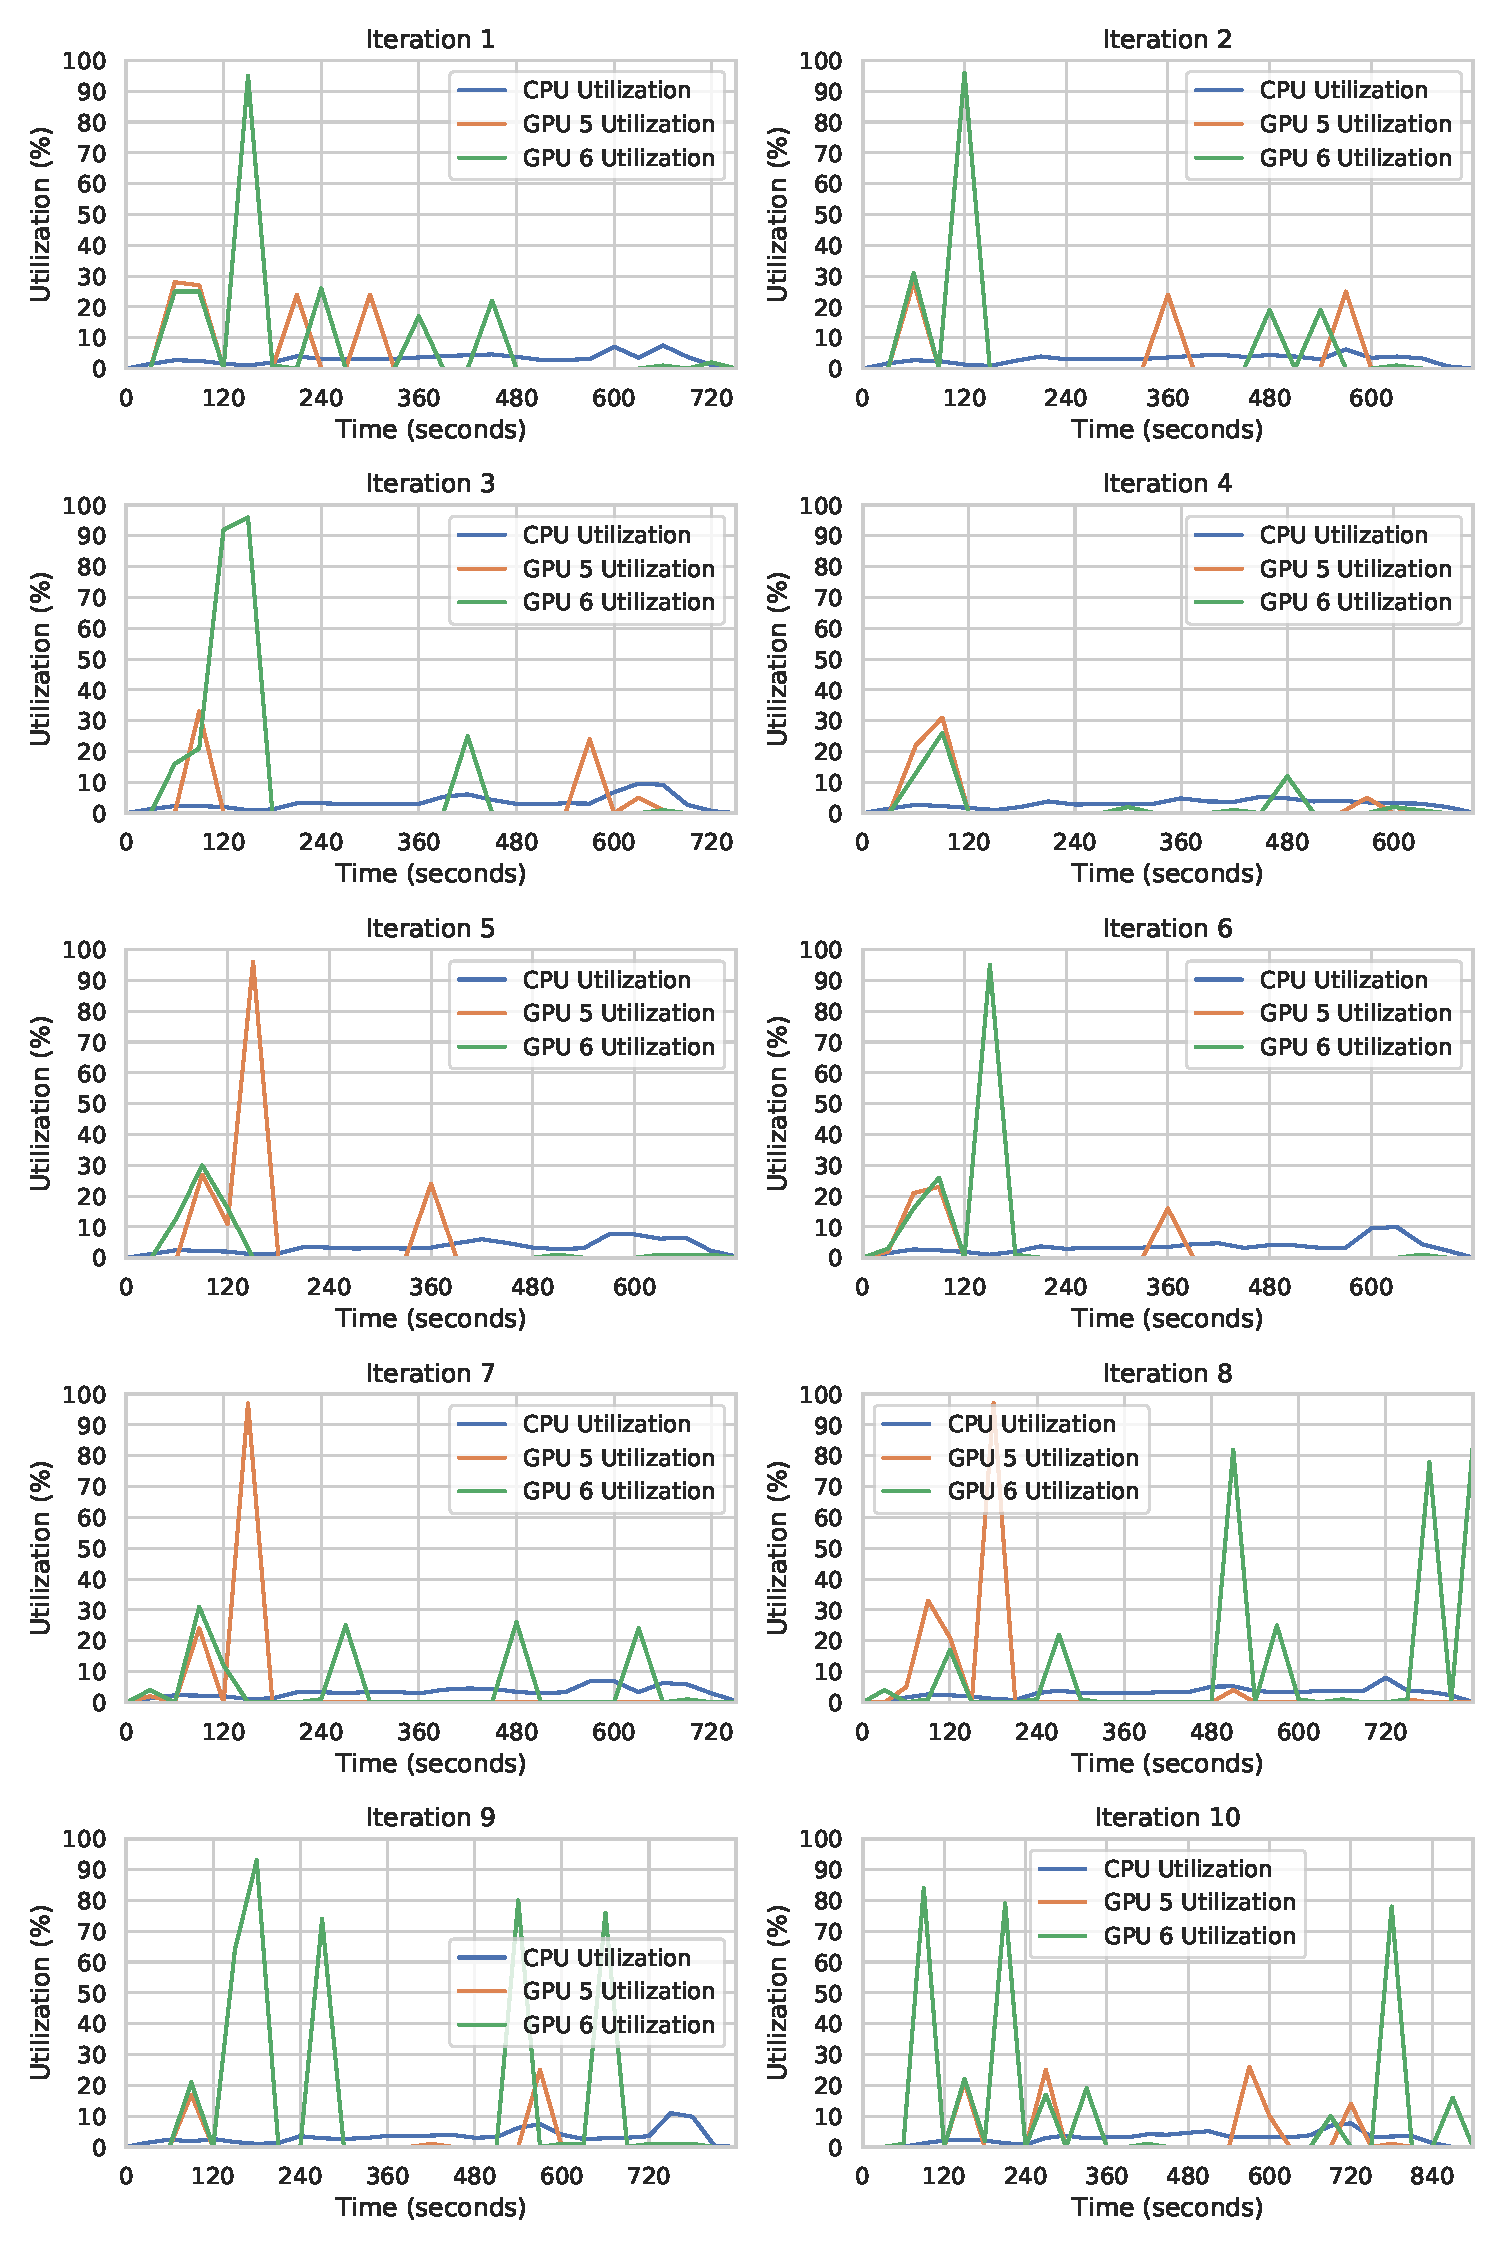
\includegraphics[scale=0.4]{images/07_evaluation/mortgage/mortgage_gpu2_performance}
\caption{Classification algorithm performance evaluation of the computing environment with 2 Apache Spark worker and GPU acceleration enabled}
\label{fig:07_mortgage_static-cpu_results}
\end{figure}

\begin{figure}[h]
\centering
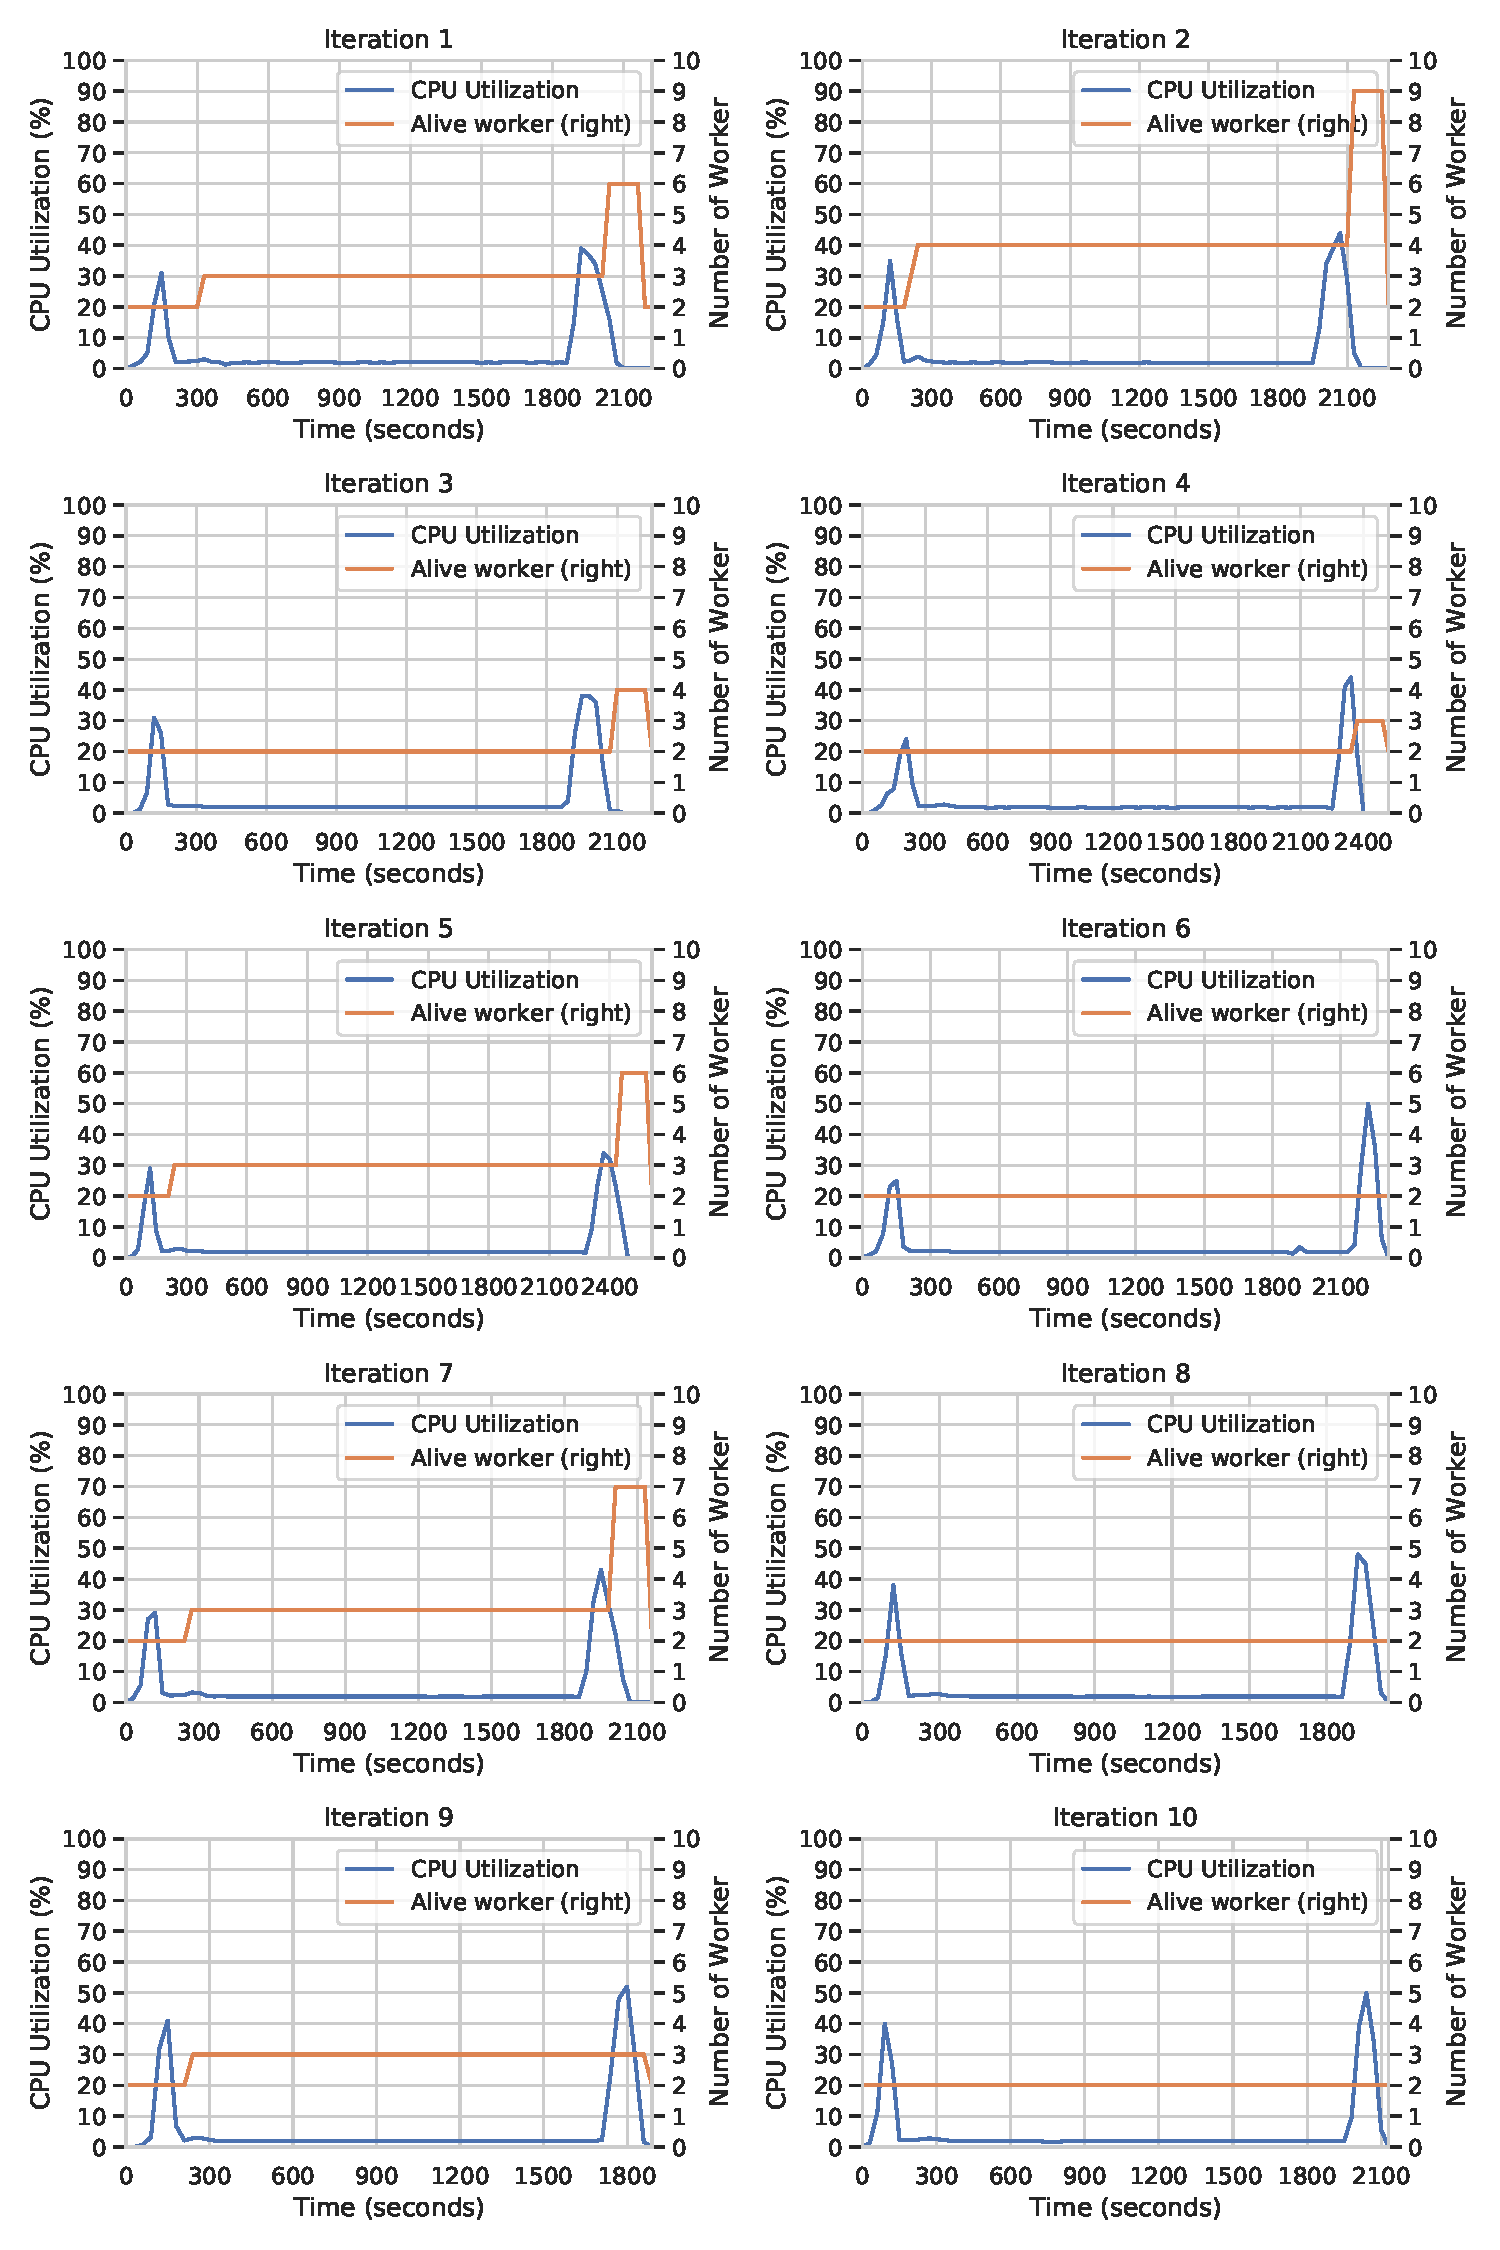
\includegraphics[scale=0.4]{images/07_evaluation/mortgage/mortgage_auto-scaler_performance}
\caption{Basic architecture of a GitLab CI/CD pipeline - Source: Authors own model, based on \cite{Gitlab2020Docs}.}
\label{fig:07_mortgage_static-cpu_results}
\end{figure}


\subsection{Regression Benchmarks}

\begin{figure}[h]
\centering
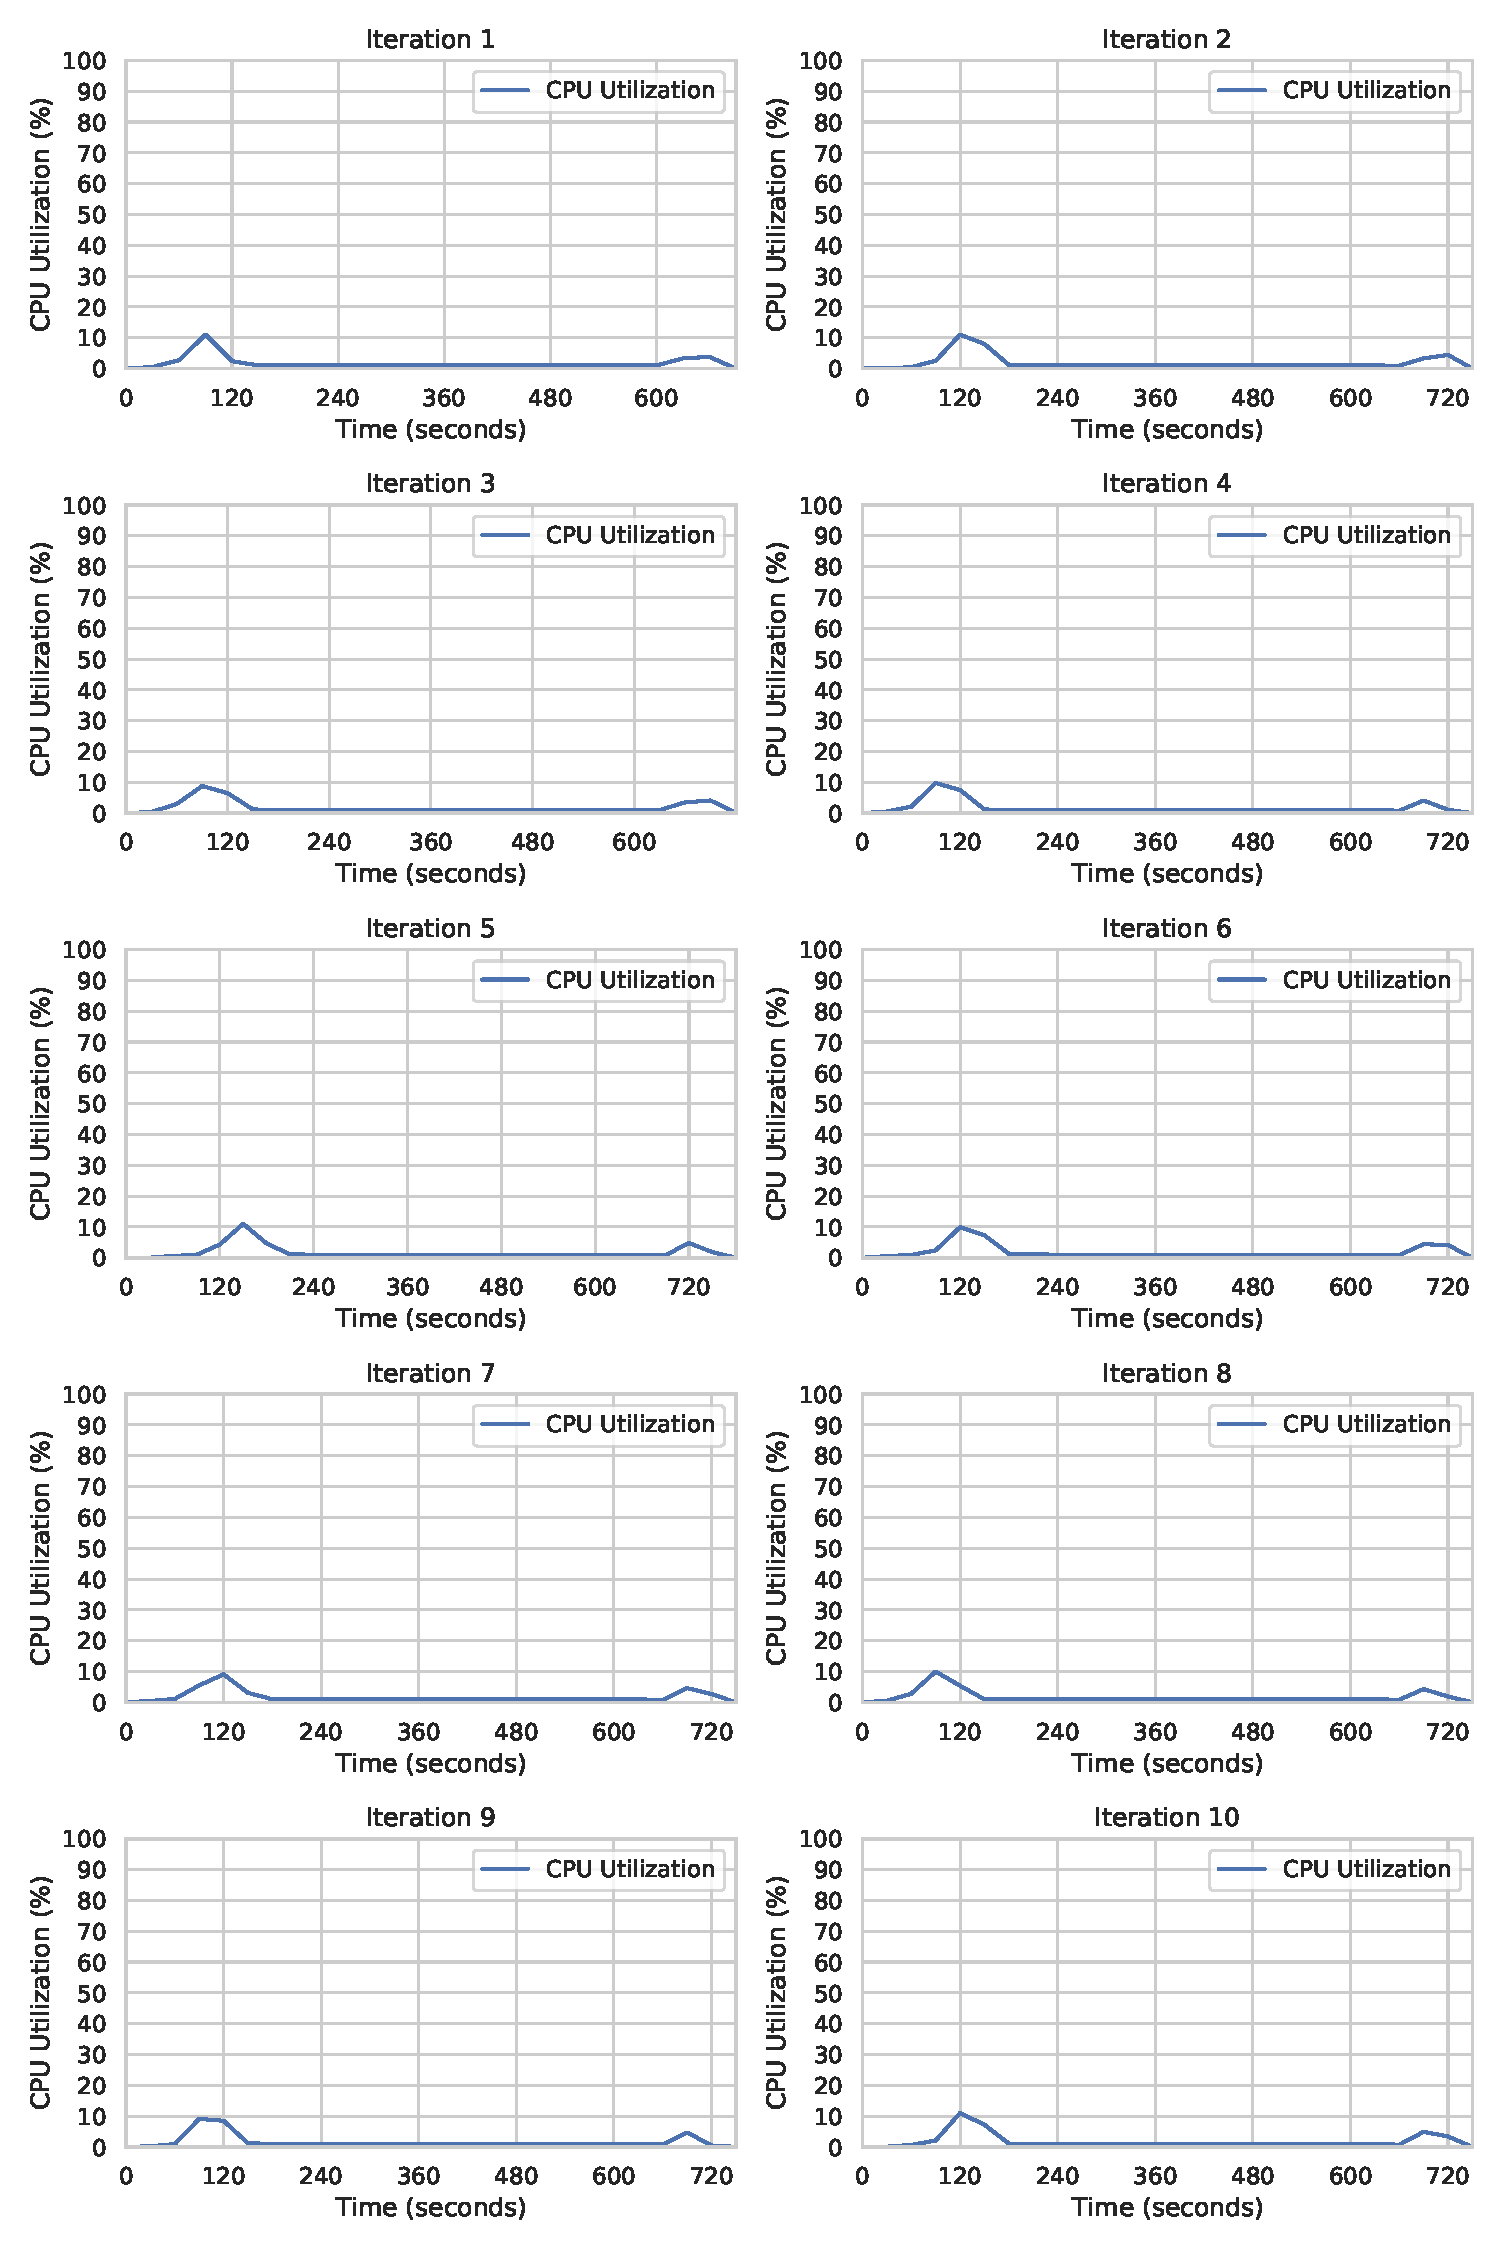
\includegraphics[scale=0.4]{images/07_evaluation/taxi/taxi_1_worker_cpu_performance}
\caption{Classification algorithm performance evaluation of the computing environment with 1 Apache Spark worker}
\label{fig:07_mortgage_static-cpu_results}
\end{figure}

\begin{figure}[h]
\centering
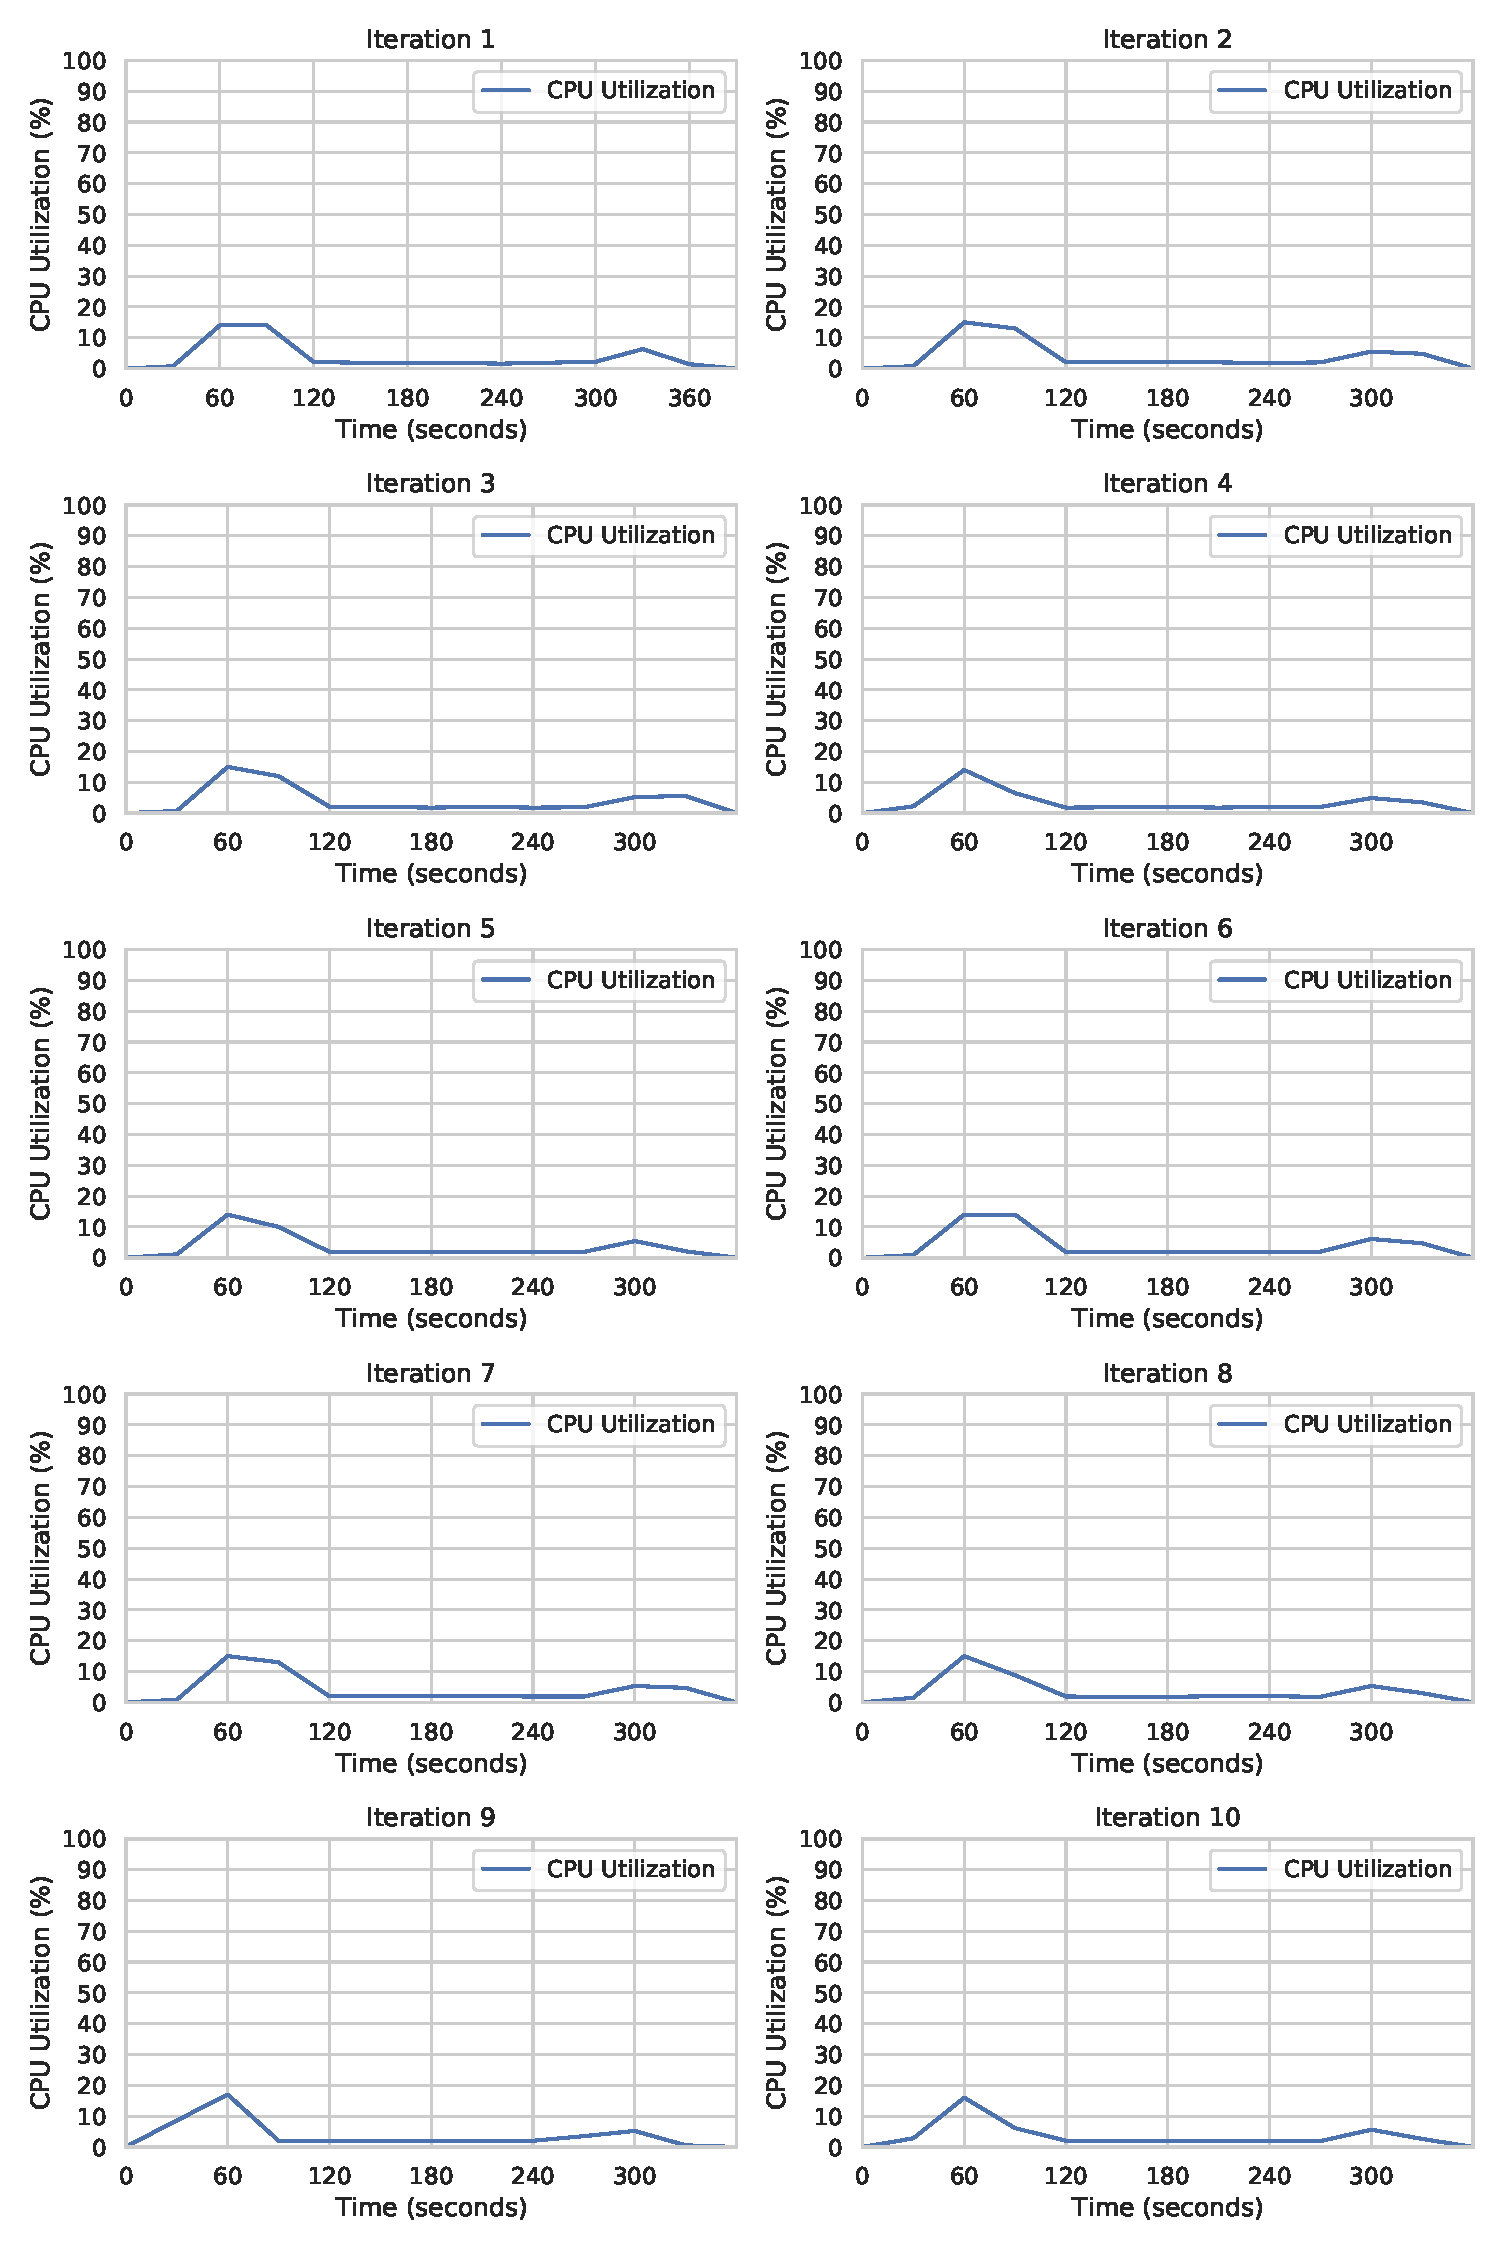
\includegraphics[scale=0.4]{images/07_evaluation/taxi/taxi_2_worker_cpu_performance}
\caption{Classification algorithm performance evaluation of the computing environment with 2 Apache Spark worker}
\label{fig:07_mortgage_static-cpu_results}
\end{figure}

\begin{figure}[h]
\centering
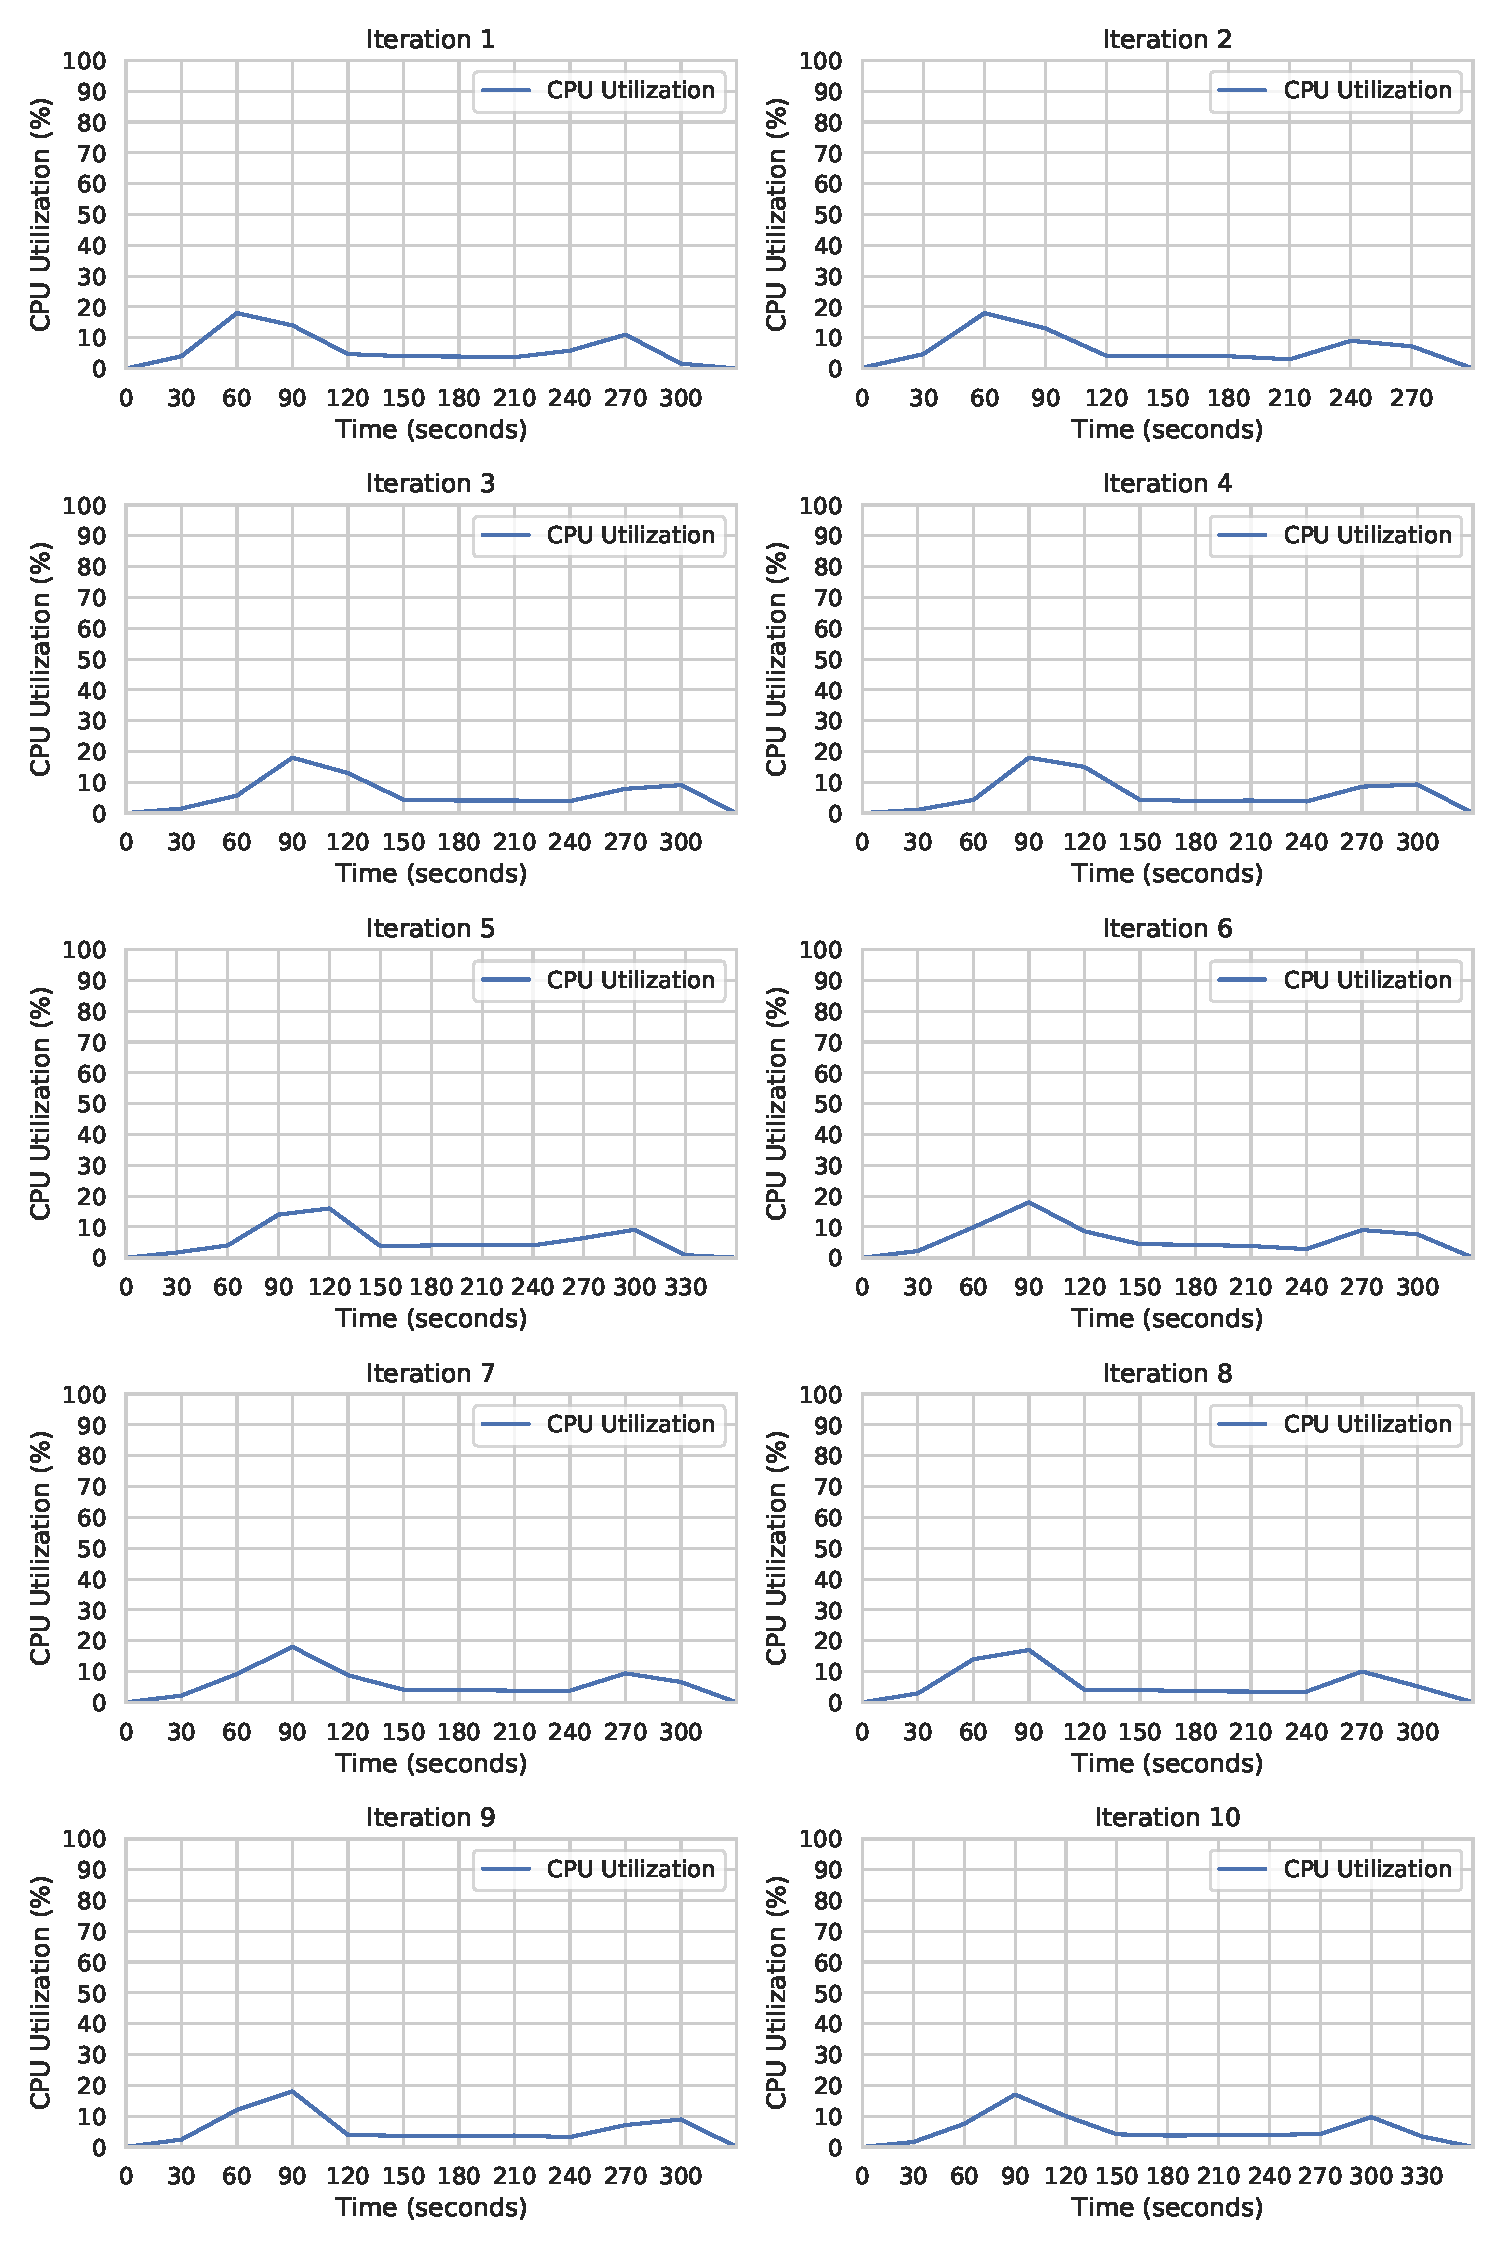
\includegraphics[scale=0.4]{images/07_evaluation/taxi/taxi_5_worker_cpu_performance}
\caption{Classification algorithm performance evaluation of the computing environment with 5 Apache Spark worker}
\label{fig:07_mortgage_static-cpu_results}
\end{figure}

\begin{figure}[h]
\centering
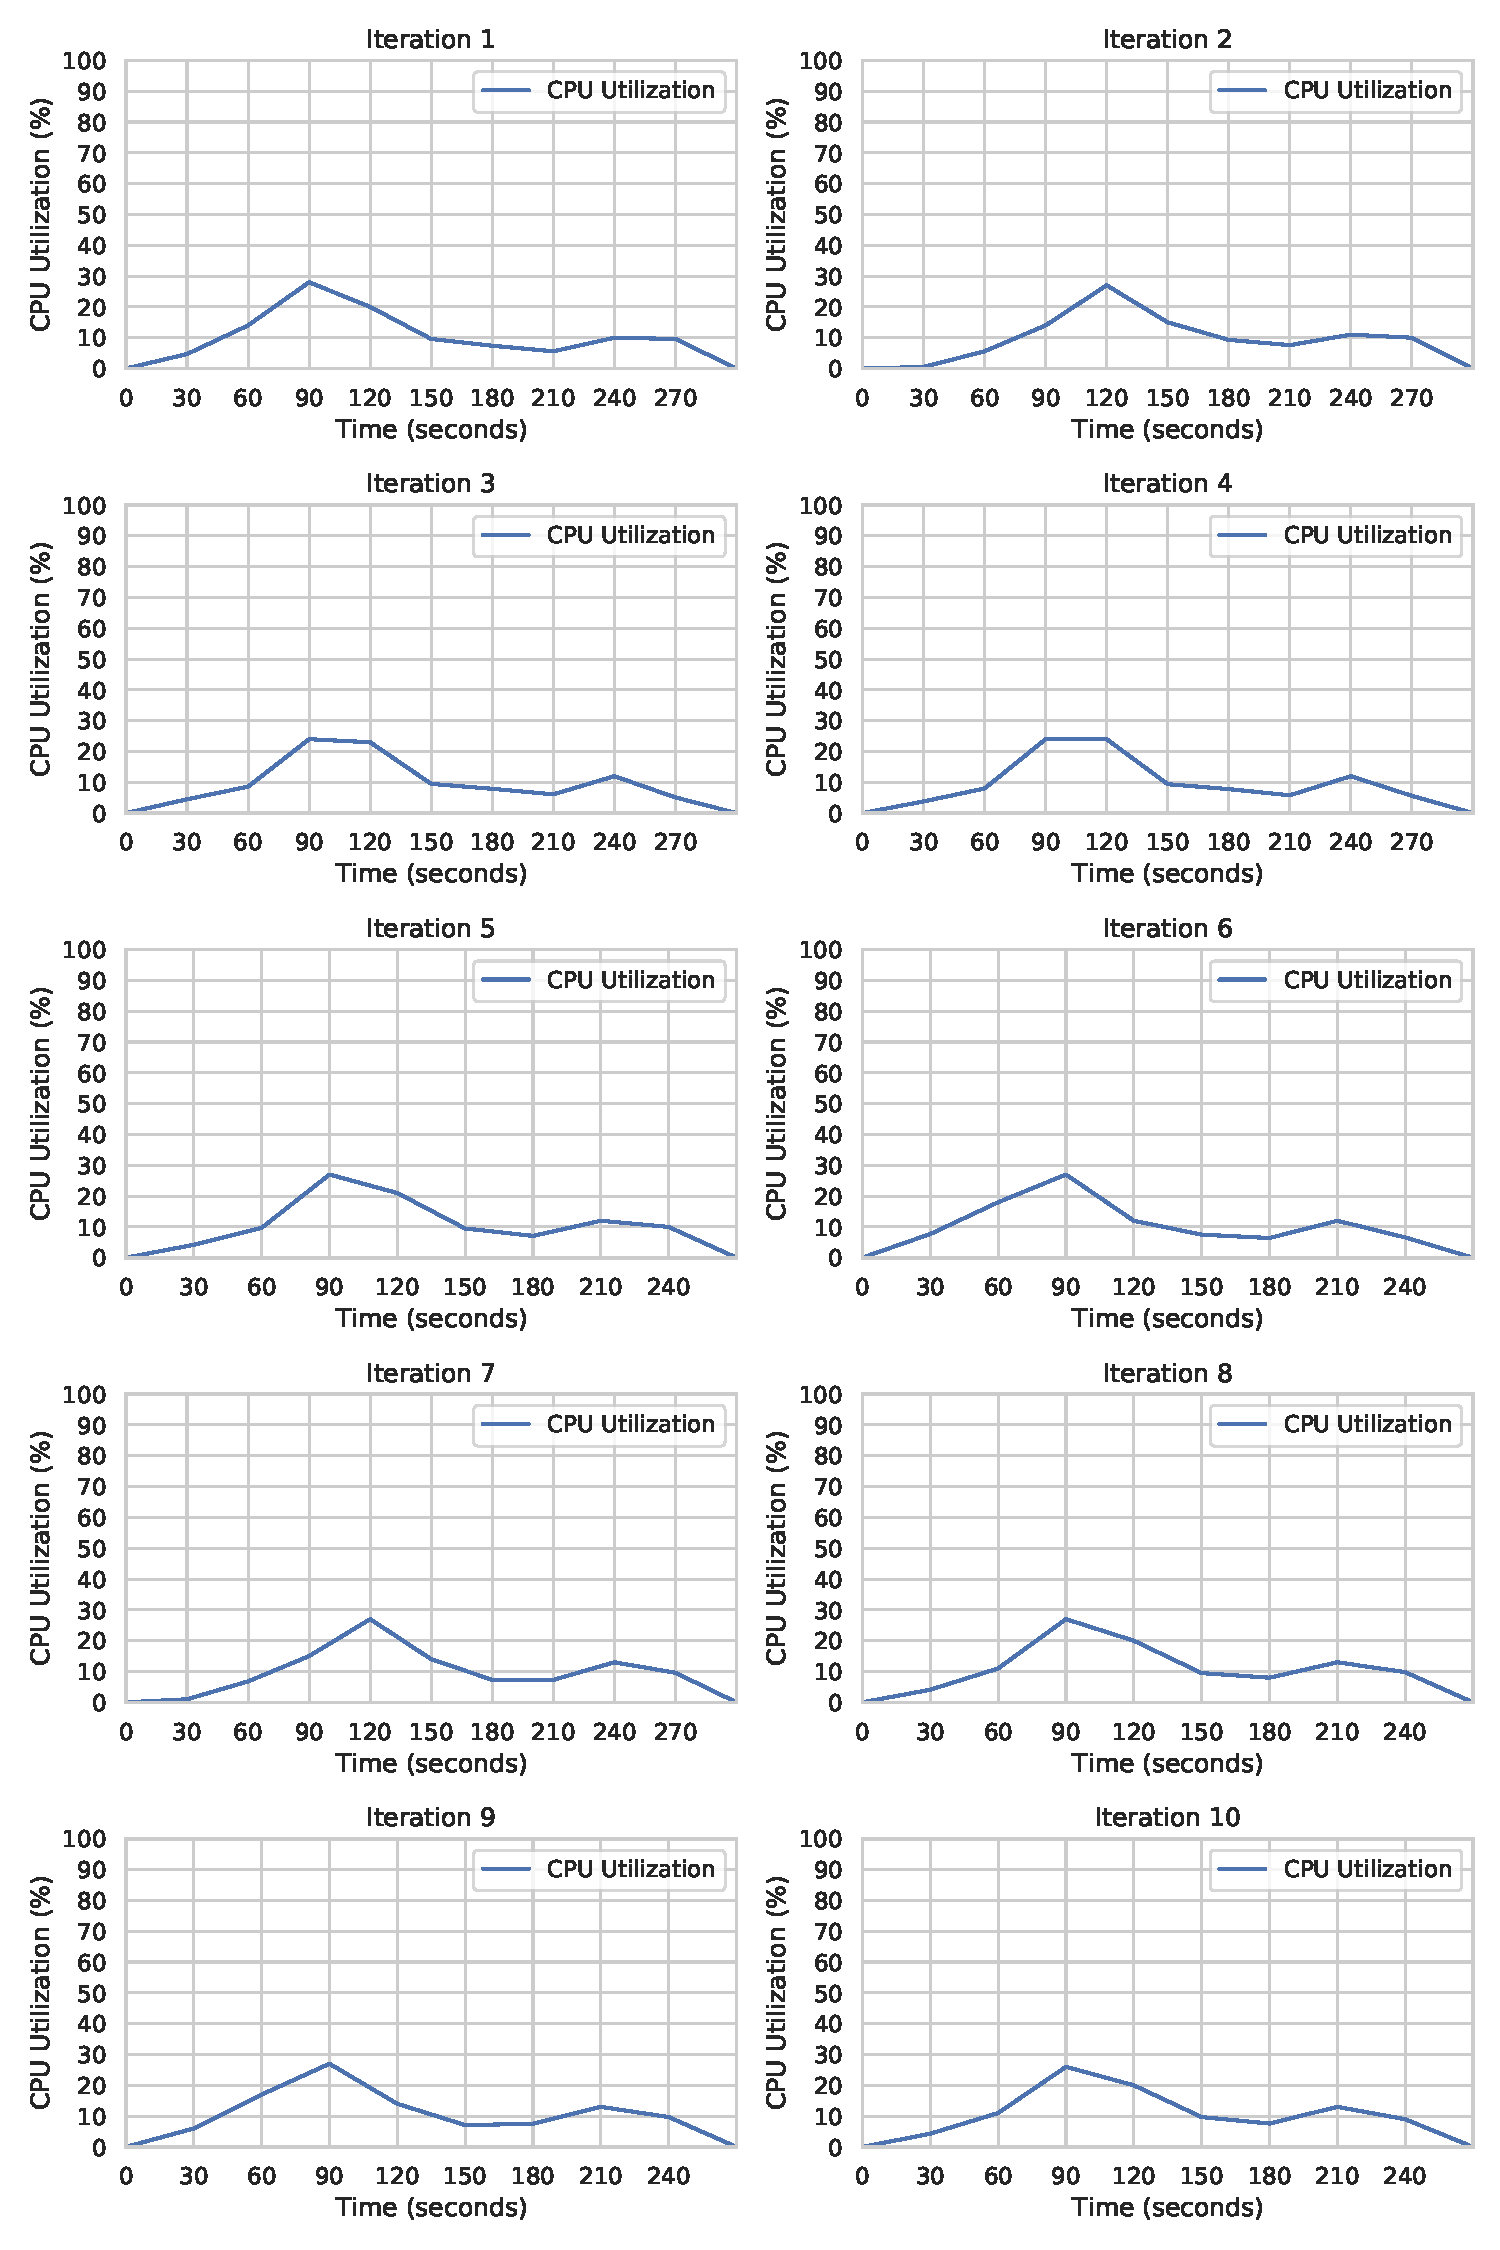
\includegraphics[scale=0.4]{images/07_evaluation/taxi/taxi_10_worker_cpu_performance}
\caption{Classification algorithm performance evaluation of the computing environment with 10 Apache Spark worker}
\label{fig:07_mortgage_static-cpu_results}
\end{figure}

\begin{figure}[h]
\centering
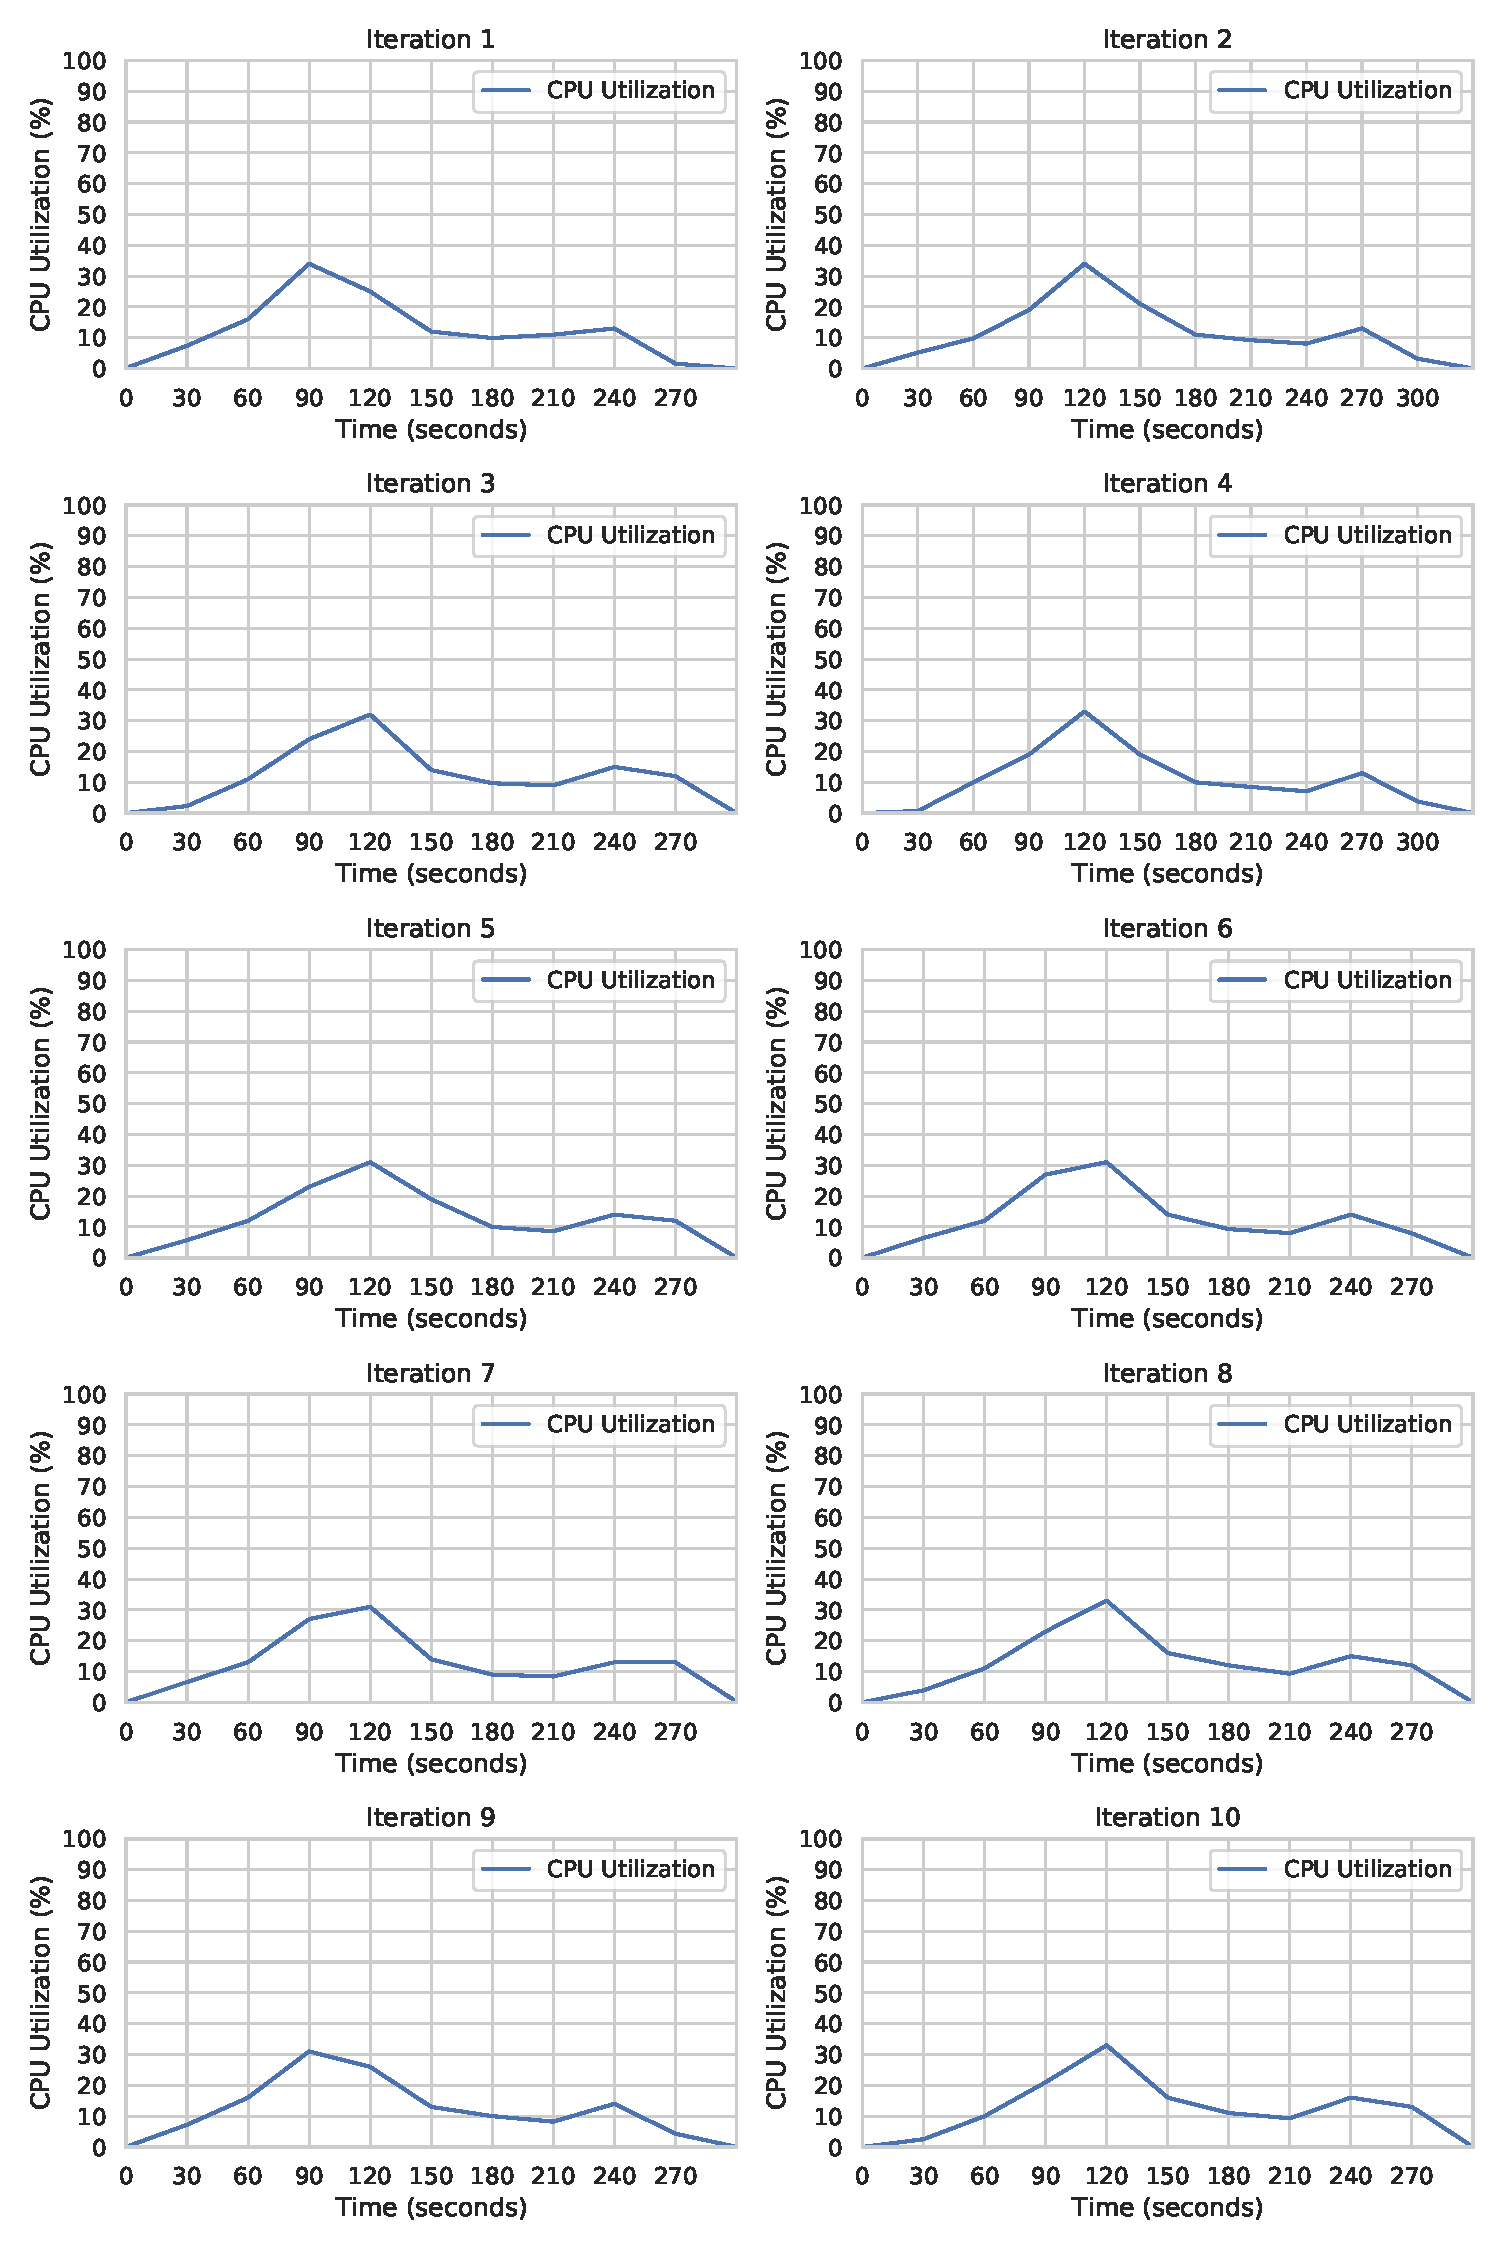
\includegraphics[scale=0.4]{images/07_evaluation/taxi/taxi_15_worker_cpu_performance}
\caption{Classification algorithm performance evaluation of the computing environment with 15 Apache Spark worker}
\label{fig:07_mortgage_static-cpu_results}
\end{figure}

\begin{figure}[h]
\centering
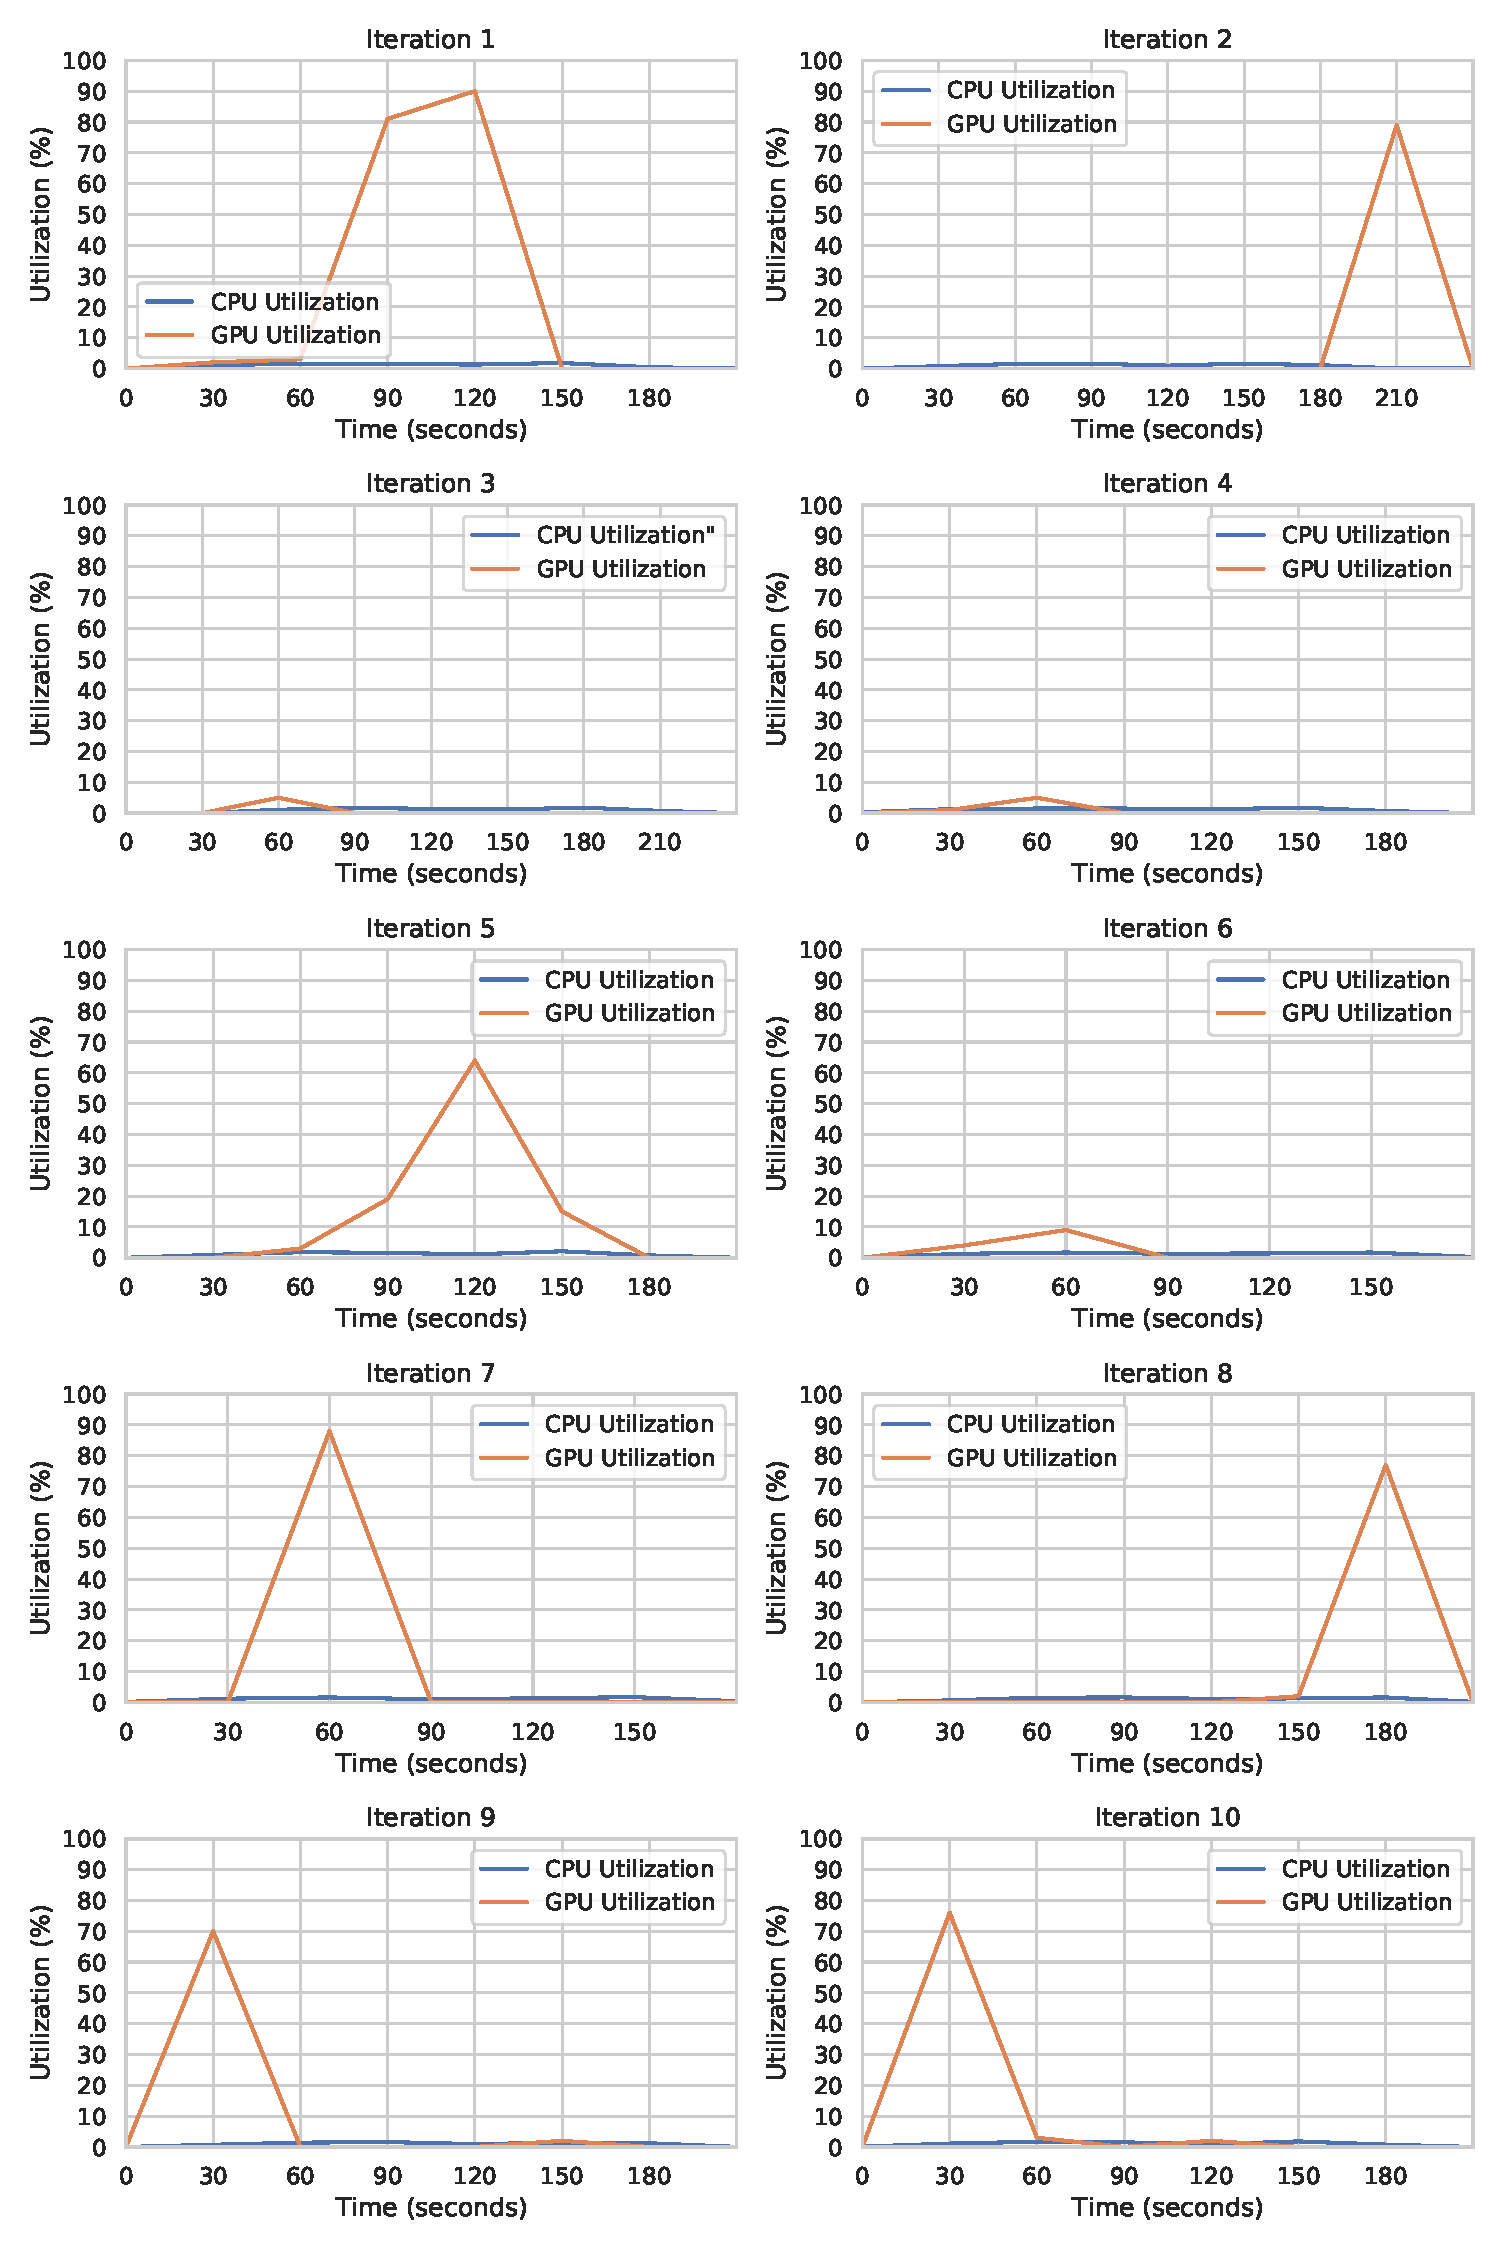
\includegraphics[scale=0.4]{images/07_evaluation/taxi/taxi_gpu1_performance}
\caption{Classification algorithm performance evaluation of the computing environment with 1 Apache Spark worker and GPU acceleration enabled}
\label{fig:07_mortgage_static-cpu_results}
\end{figure}

\begin{figure}[h]
\centering
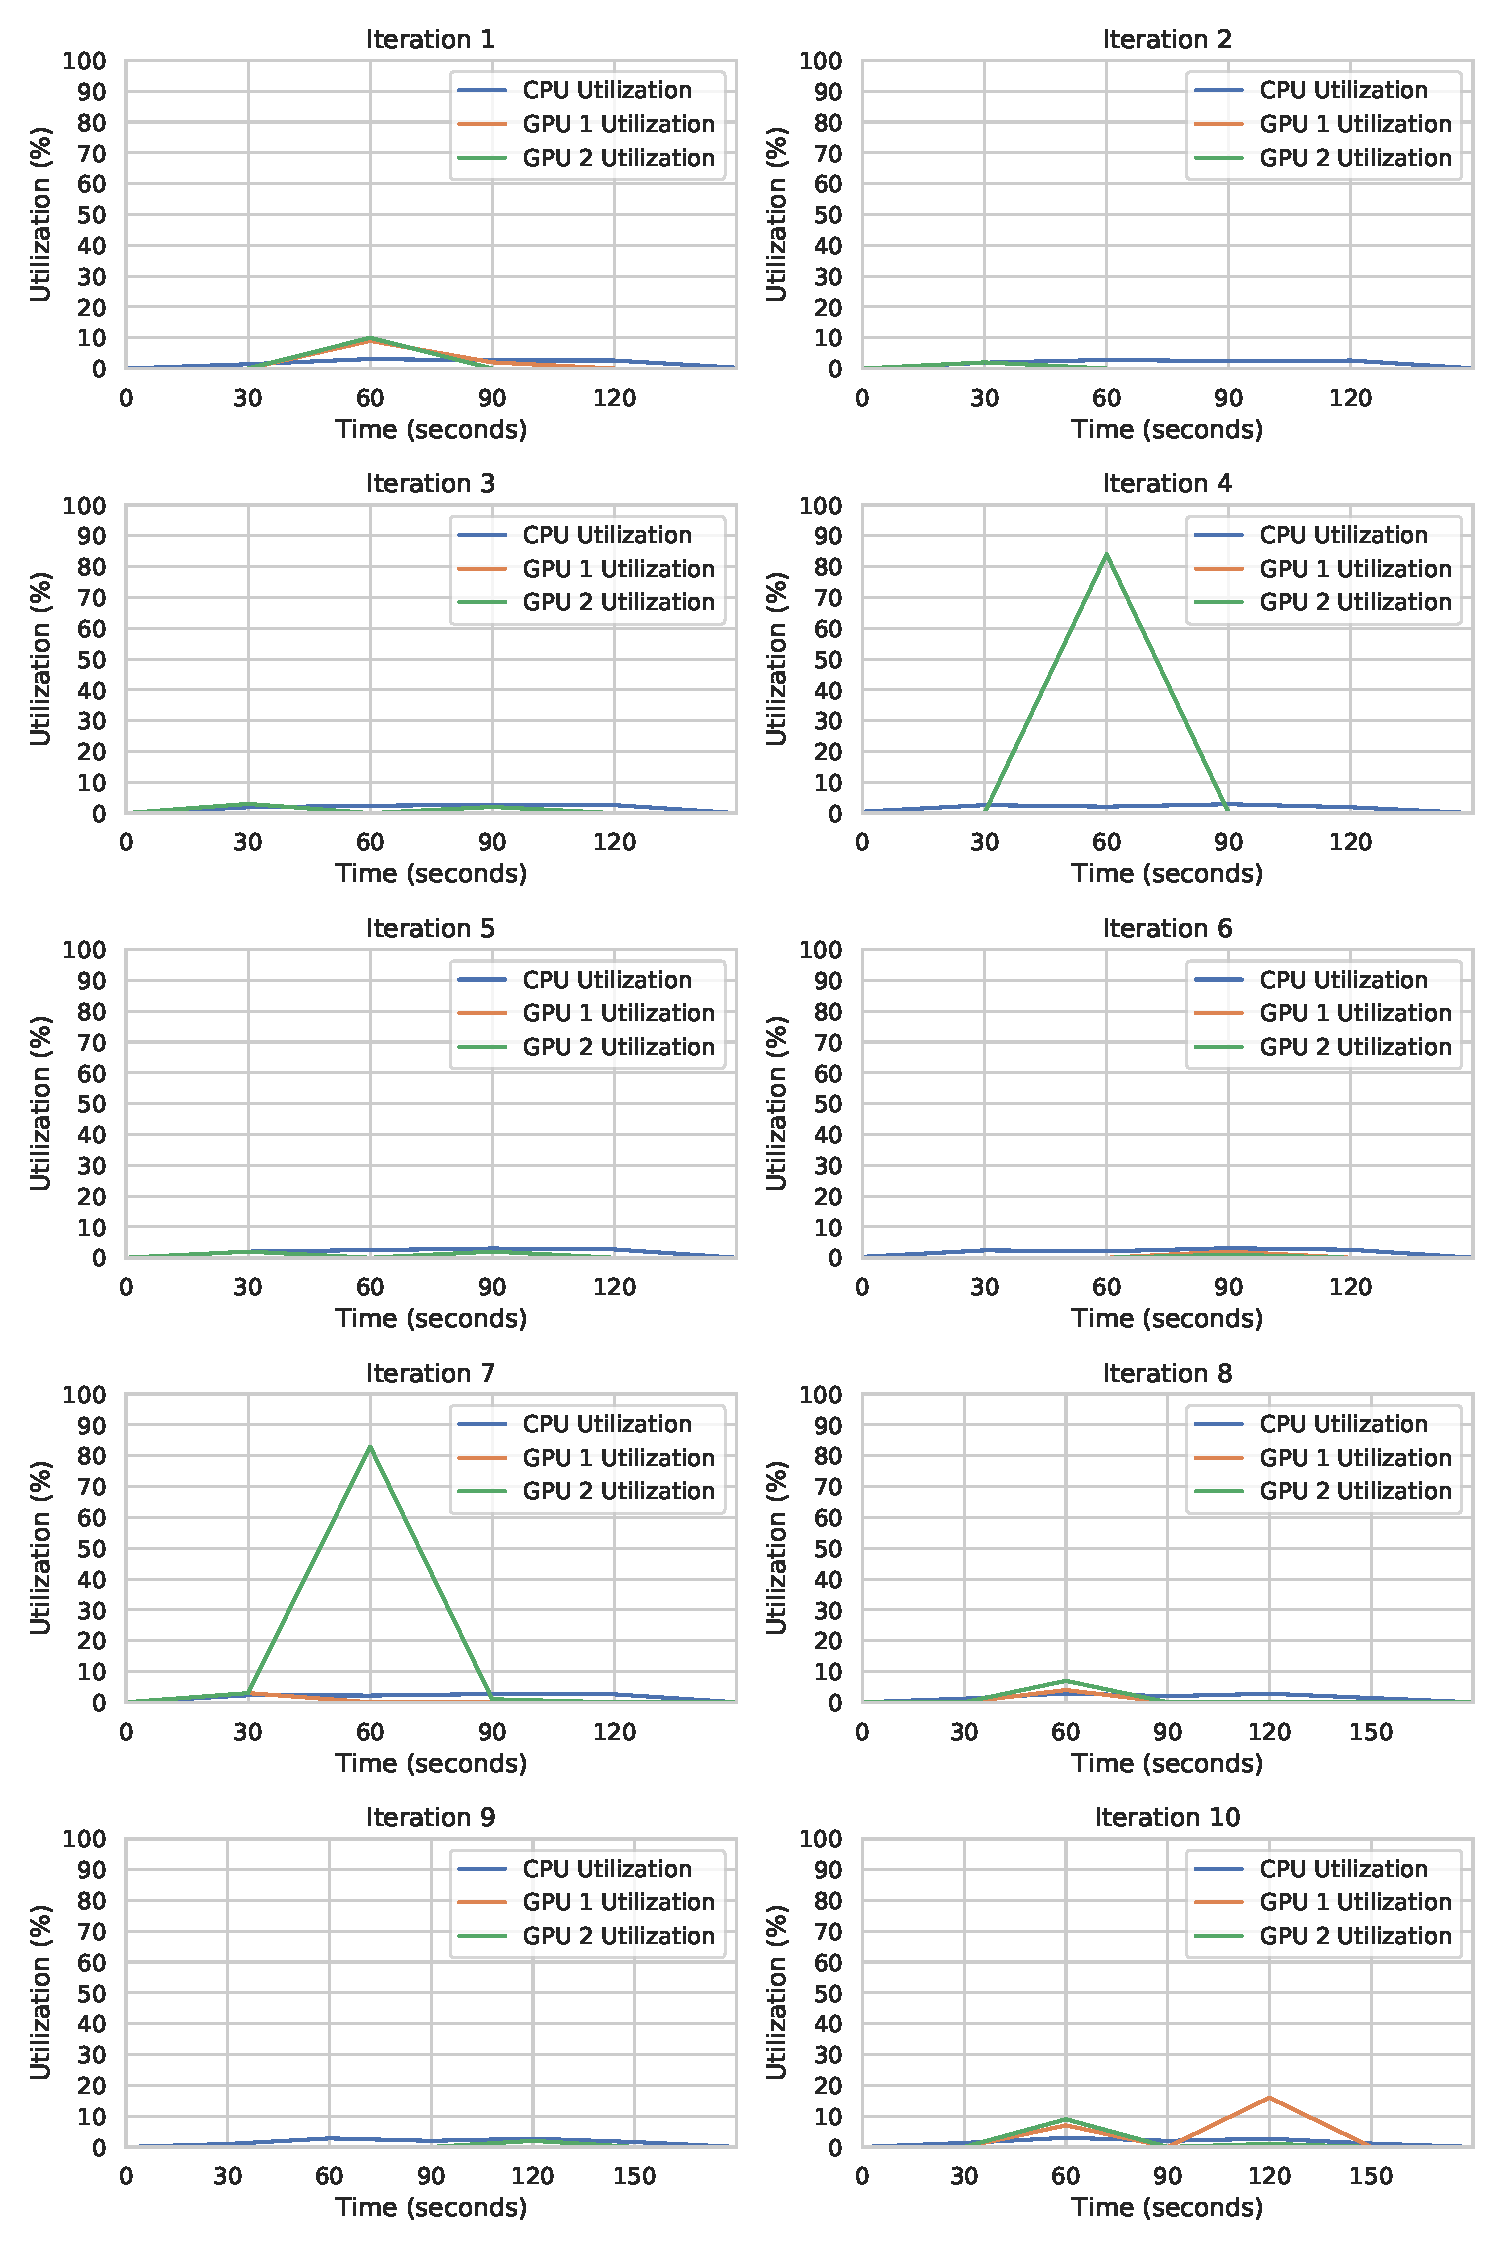
\includegraphics[scale=0.4]{images/07_evaluation/taxi/taxi_gpu2_performance}
\caption{Classification algorithm performance evaluation of the computing environment with 2 Apache Spark worker and GPU acceleration enabled}
\label{fig:07_mortgage_static-cpu_results}
\end{figure}

\begin{figure}[h]
\centering
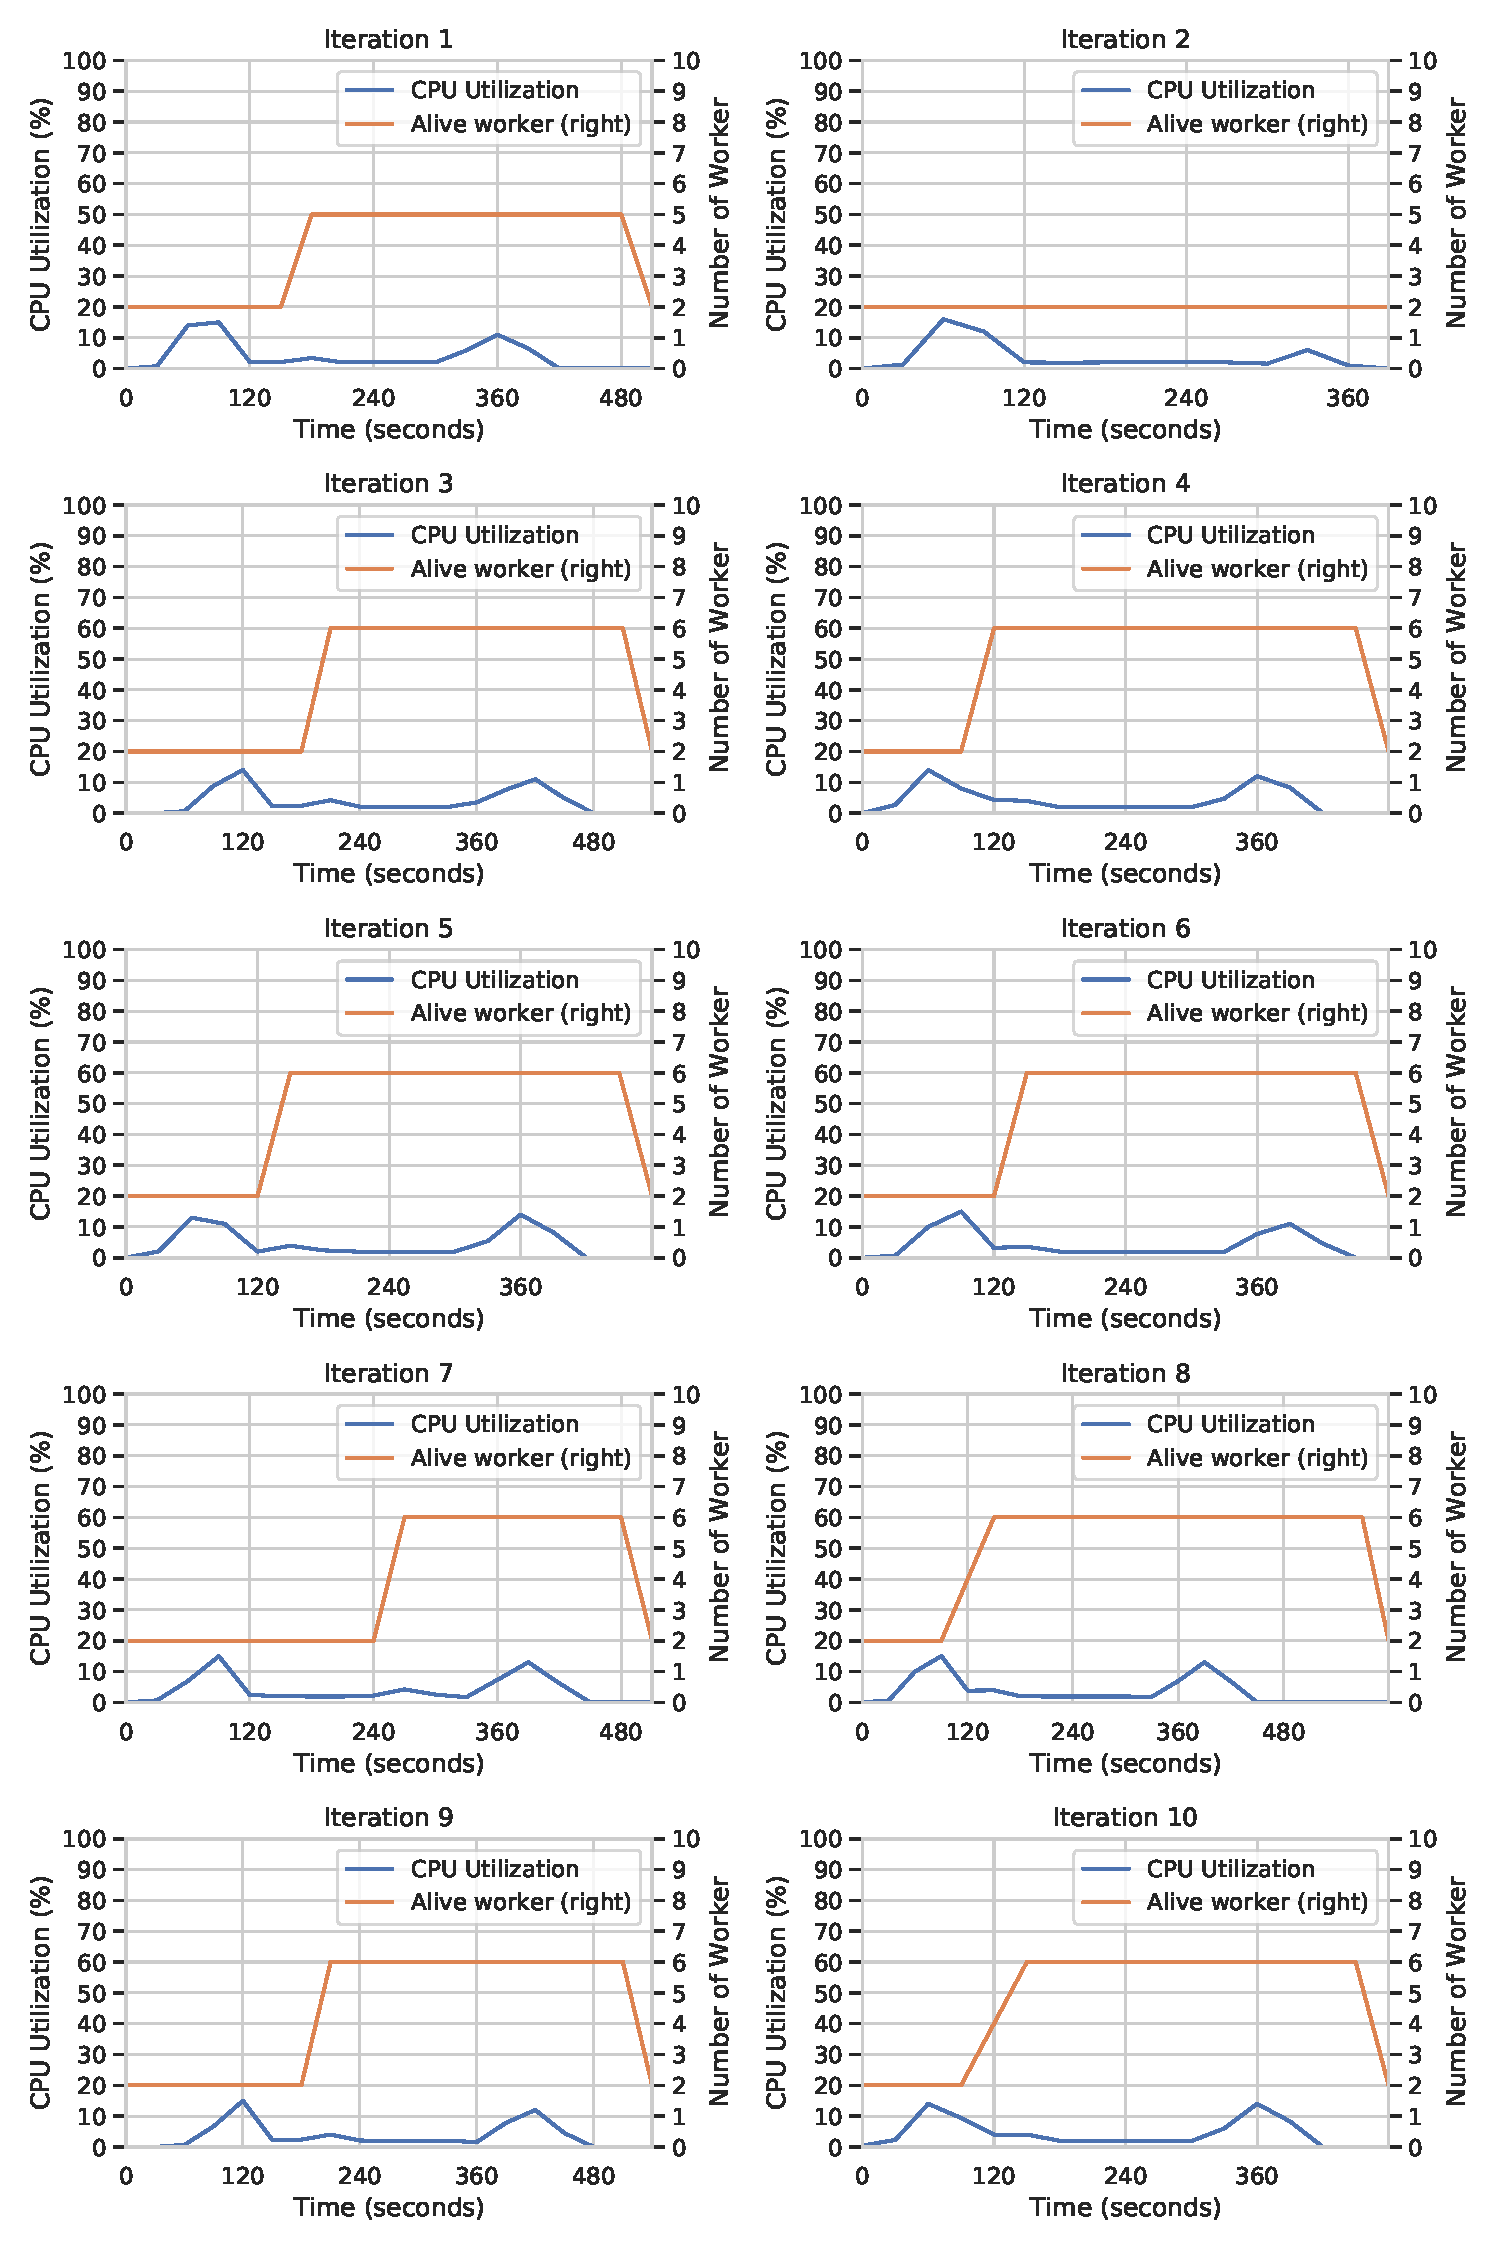
\includegraphics[scale=0.4]{images/07_evaluation/taxi/taxi_auto-scaler_performance}
\caption{Basic architecture of a GitLab CI/CD pipeline - Source: Authors own model, based on \cite{Gitlab2020Docs}.}
\label{fig:07_mortgage_static-cpu_results}
\end{figure}



\IfDefined{printindex}{\printindex}
\IfDefined{printnomenclature}{\printnomenclature}



%% Dokument ENDE %%%%%%%%%%%%%%%%%%%%%%%%%%%%%%%%%%%%%%%%%%%%%%%%%%%%%%%%%%
\end{document}

